\documentclass[11pt]{article}
% Shared preamble — owned by LEAD. Section authors: do not add packages; request them in NOTES-<owner>.md.
\usepackage[T1]{fontenc}
\usepackage[utf8]{inputenc}
\usepackage{amsmath,mathtools,amsthm}
\IfFileExists{newtxtext.sty}{%
  \usepackage{newtxtext}\usepackage[varvw]{newtxmath}%
}{%
  \usepackage{mathptmx}\usepackage{amssymb}%
}
\usepackage[letterpaper,margin=1.05in,headheight=14pt]{geometry}
\usepackage{thmtools}
\usepackage{bm}
\usepackage[dvipsnames]{xcolor}
\usepackage{microtype}
\usepackage{booktabs,array,tabularx}
\usepackage{graphicx}
\usepackage{caption,subcaption}
\usepackage[shortlabels]{enumitem}
\usepackage{algorithm}
\usepackage[noend]{algpseudocode}
\usepackage{tikz}
\usetikzlibrary{arrows.meta,positioning,calc,shapes.geometric,fit,backgrounds,decorations.pathreplacing}
\usepackage[numbers,sort&compress]{natbib}
\usepackage{fancyhdr}
\usepackage[colorlinks=true,linkcolor=MidnightBlue,citecolor=MidnightBlue,urlcolor=MidnightBlue]{hyperref}
\usepackage[capitalise,noabbrev,nameinlink]{cleveref}

\captionsetup{font=small,labelfont=bf,labelsep=period}
\setlength{\parskip}{0pt}
\setlist{itemsep=2pt,topsep=4pt}

% ---- theorem environments (one shared counter) ----
\theoremstyle{plain}
\newtheorem{theorem}{Theorem}
\newtheorem{proposition}[theorem]{Proposition}
\newtheorem{lemma}[theorem]{Lemma}
\newtheorem{corollary}[theorem]{Corollary}
\theoremstyle{definition}
\newtheorem{definition}[theorem]{Definition}
\newtheorem{assumption}{Assumption}
\renewcommand{\theassumption}{A\arabic{assumption}}
\newtheorem{example}[theorem]{Example}
\theoremstyle{remark}
\newtheorem{remark}[theorem]{Remark}
\crefname{assumption}{Assumption}{Assumptions}
\crefname{algorithm}{Algorithm}{Algorithms}
\crefname{appendix}{Appendix}{Appendices}

% ---- notation macros (see SPEC.md) ----
\newcommand{\E}{\mathbb{E}}
\renewcommand{\Pr}{\mathbb{P}}
\newcommand{\Var}{\operatorname{Var}}
\newcommand{\Cov}{\operatorname{Cov}}
\newcommand{\ind}[1]{\mathbf{1}\!\left\{#1\right\}}
\newcommand{\Kset}{[K]}
\newcommand{\Hset}{\mathcal{H}}
\newcommand{\Hobs}{\mathcal{H}_{+}}          % nonzero histories
\newcommand{\zero}{\mathbf{0}}
\newcommand{\h}{\bm{h}}
\newcommand{\nzero}{n_{\zero}}
\newcommand{\Nhat}{\widehat{N}}
\newcommand{\Link}{\Lambda}
\newcommand{\Linkhat}{\widehat{\Lambda}}
\newcommand{\Lop}{\mathcal{T}}               % linkage operator T(delta, eps)
\newcommand{\dirichlet}{\operatorname{Dir}}
\newcommand{\DP}{\operatorname{DP}}
\newcommand{\Bern}{\operatorname{Bernoulli}}
\newcommand{\Pois}{\operatorname{Poisson}}
\newcommand{\Mult}{\operatorname{Multinomial}}
\newcommand{\Bin}{\operatorname{Binomial}}
\newcommand{\supp}{\operatorname{supp}}
\newcommand{\logit}{\operatorname{logit}}
\newcommand{\argmin}{\operatorname*{arg\,min}}
\newcommand{\argmax}{\operatorname*{arg\,max}}
\newcommand{\rvic}{\rho_{\mathrm{vic}}}
\newcommand{\rpol}{\rho_{\mathrm{pol}}}
\newcommand{\rcls}{\rho_{\mathrm{cls}}}
\newcommand{\rsub}{\rho_{\mathrm{sub}}}
\newcommand{\nFBI}{n_{\mathrm{FBI}}}
\newcommand{\factcheck}[1]{\textcolor{red}{[FACT-CHECK: #1]}}
\newcommand{\todo}[1]{\textcolor{orange}{[TODO: #1]}}

% ---- Paper 2 (contagion) notation macros ----
\newcommand{\Hist}{\mathcal{F}}            % history / filtration F_t
\newcommand{\Amat}{\bm{A}}                 % branching matrix [alpha_kj]
\newcommand{\Imat}{\bm{I}}
\newcommand{\Mmat}{\bm{M}}                 % contagion multiplier (I - A)^{-1}
\newcommand{\spr}{\varrho}                 % spectral radius
\newcommand{\Rker}{\bm{R}}                 % resolvent kernel
\newcommand{\Phik}{\bm{\Phi}}              % excitation kernel matrix
\newcommand{\dN}{\mathrm{d}N}
\newcommand{\dd}{\mathrm{d}}
\newcommand{\Lam}{\Lambda}                 % compensator


\hypersetup{
  pdftitle={Shock and Contagion: Self-Exciting Point Processes for Surges in Antisemitic Incidents},
  pdfauthor={Kornstein Lab for Antisemitism Research},
  pdfsubject={Methods paper with simulation study on synthetic data and a pre-registered analysis plan; no empirical estimates from real incident data},
  pdfkeywords={Hawkes process, self-exciting point process, contagion, identification, under-reporting, surge attribution, forecasting, hate crime, antisemitism}
}

\begin{document}

% ======================= title block =======================
\thispagestyle{plain}
\begingroup
\raggedright
{\footnotesize\scshape\color{LabAccent}Kornstein Lab for Antisemitism Research%
 \enspace\textcolor{LabRule}{|}\enspace\textcolor{LabGrey}{Methods paper}%
 \enspace\textcolor{LabRule}{|}\enspace\textcolor{LabGrey}{Companion to
 \textup{\itshape The Dark Figure}}\par}
\vspace{5pt}
{\color{LabNavy}\rule{\textwidth}{1.3pt}}\par
\vspace{16pt}
{\fontsize{34}{38}\selectfont\color{LabNavy}Shock and Contagion%
 \textsuperscript{\normalsize\color{LabAccent}$\ast$}\par}
\vspace{8pt}
{\fontsize{15.5}{19}\selectfont\color{LabInk}Self-Exciting Point Processes
 for Surges in Antisemitic Incidents\par}
\vspace{14pt}
{\normalsize\color{LabInk}Kornstein Lab for Antisemitism Research\par}
\vspace{2pt}
{\small\color{LabGrey}November 2026\par}
\vspace{8pt}
\endgroup
% A schematic conditional intensity: one salient external event (orange),
% followed by a cascade. Title-page ornament; not data.
\IfFileExists{figures/fig-title-strip.tex}{% =====================================================================
%  Title-page ornament (LEAD): a schematic conditional intensity across the
%  text width. ONE seeded synthetic realisation (numpy default_rng(9);
%  mu = 0.2, n = 0.5, kernel rate 1.0, one shock at t = 57 with 10 expected
%  direct incidents, response rate 0.6), drawn exactly in TikZ from its event
%  times. It is decoration, not data.
% =====================================================================
\par\noindent
\begin{tikzpicture}[x=0.0098\textwidth,y=0.112cm]
  \def\kmu{0.2}\def\kn{0.5}\def\kbeta{1.0}\def\kgam{0.6}\def\kjump{6.0}
  \xdef\tp{0}\xdef\Hs{0}\xdef\Ss{0}
  \foreach \t/\k in {0.56/1,2.66/1,6.52/1,27.97/1,29.92/1,31.56/1,43.72/1,
      44.97/1,48.49/1,55.45/1,55.47/1,56.40/1,57.00/2,57.09/1,57.11/1,57.24/1,
      57.25/1,57.41/1,57.71/1,57.72/1,57.80/1,58.36/1,58.56/1,58.67/1,58.72/1,
      58.73/1,59.11/1,59.39/1,59.49/1,60.21/1,60.24/1,60.31/1,60.79/1,61.12/1,
      61.21/1,61.43/1,61.46/1,63.57/1,70.53/1,70.82/1,71.01/1,71.36/1,71.61/1,
      74.07/1,74.51/1,76.67/1,77.75/1,78.26/1,78.46/1,83.06/1,84.33/1,86.04/1,
      88.29/1,91.28/1,91.54/1,91.82/1,92.08/1,98.33/1,98.62/1,98.77/1,99.17/1,
      100/0}{
    \fill[LabTint]
      plot[domain=\tp:\t,samples=10]
        (\x,{\kmu+\Ss*exp(-\kgam*(\x-\tp))+\Hs*exp(-\kbeta*(\x-\tp))})
      -- (\t,0) -- (\tp,0) -- cycle;
    \draw[LabNavyMid,line width=0.45pt,line join=round]
      plot[domain=\tp:\t,samples=10]
        (\x,{\kmu+\Ss*exp(-\kgam*(\x-\tp))+\Hs*exp(-\kbeta*(\x-\tp))});
    \pgfmathsetmacro{\Hn}{\Hs*exp(-\kbeta*(\t-\tp))+(\k==1)*\kn*\kbeta}
    \pgfmathsetmacro{\Sn}{\Ss*exp(-\kgam*(\t-\tp))+(\k==2)*\kjump}
    \pgfmathsetmacro{\Lold}{\kmu+\Ss*exp(-\kgam*(\t-\tp))+\Hs*exp(-\kbeta*(\t-\tp))}
    \pgfmathsetmacro{\Lnew}{\kmu+\Sn+\Hn}
    \ifnum\k>0 \draw[LabNavyMid,line width=0.45pt] (\t,\Lold) -- (\t,\Lnew);\fi
    \ifnum\k=1 \draw[LabNavyLight,line width=0.4pt] (\t,-0.5) -- (\t,-1.6);\fi
    \xdef\tp{\t}\xdef\Hs{\Hn}\xdef\Ss{\Sn}
  }
  \draw[LabRule,line width=0.4pt] (0,0) -- (100,0);
  \fill[LabAccent] (57,-1.05) -- ++(0.32,0.55) -- ++(0.32,-0.55) -- ++(-0.32,-0.55) -- cycle;
\end{tikzpicture}\par
\vspace{5pt}}{}
\begingroup
\renewcommand{\thefootnote}{\ensuremath{\ast}}
\footnotetext[1]{\textbf{Status.} Methods paper; simulation study on
synthetic data; pre-registered analysis plan; no empirical estimates. Every
number in \cref{sec:simulation} is computed from synthetic data with known
ground truth; the real-data analysis of \cref{sec:plan} is pre-registered and
has not been carried out. The companion paper \citep{kornsteinlab2026darkfigure}
estimates how many incidents go unrecorded; this paper uses its output.}
\endgroup

% ======================= abstract =======================
\begin{tcolorbox}[enhanced,breakable,colback=LabTint,frame hidden,boxrule=0pt,
  sharp corners,left=12pt,right=12pt,top=9pt,bottom=9pt,
  borderline west={2pt}{0pt}{LabNavy},before skip=4pt,after skip=12pt]
\begin{abstract}
After salient external events, how much of a surge in antisemitic incidents
is direct reaction, how much is contagion, and does online hostility spill
offline? We model incident streams as a multivariate Hawkes process with
exogenous shocks. Within a stream, the autocorrelation of counts cannot
separate contagion from unrecorded shocks, although dominant
cross-excitation is identifiable at second order; a rigid background
manufactures contagion; and under-reporting attenuates it through an
invertible map. We decompose post-event surges into background, direct and
contagion parts. The alert rule is Bayes-optimal given the model's state,
not with a plug-in state under reporting delays. Synthetic-data simulations
evaluate EM, attribution, the boundary test, the thinning correction and a
plug-in alert; Bayesian shrinkage, time-rescaling diagnostics, an
imputation-based alert, sup-tests and nonparametric kernels were not
evaluated. Without contagion, a constant background yields branching ratios
of up to 0.63; for rare large shocks maximum likelihood settles 0.06--0.07
below the second-order value even with $T=10{,}000$. Known event times
largely removed the artefact where tested; a single spline background did
not. The dark-figure correction restores coverage unless excitation is weak
and recording poor, and a 30--50\% error in the recording probability sets a floor under its precision that more data
cannot lower. Forecasts that ignore future external events under-forecast;
forecasts that integrate over the event process are calibrated when windows
are pooled. No forecaster can time new events, which limits recall rather
than pooled calibration. We pre-register a real-data analysis and report no
empirical estimates.
\end{abstract}
\keywords{Hawkes processes; self-exciting point processes; contagion;
identification; under-reporting; surge attribution; early warning; hate
crime; antisemitism.}
\end{tcolorbox}
\suppressfloats[t]

% ======================= body =======================
% Figure 1 (cluster representation) and Table 1 (notation) are \input from
% sections/01-introduction.tex so that they float next to their first mention.
\IfFileExists{sections/01-introduction.tex}{\section{Introduction}\label{sec:intro}

Antisemitic incidents do not arrive at a steady rate. They come in surges,
and surges often follow salient external events. In the United Kingdom, the
Community Security Trust (CST) recorded an average of five antisemitic
incidents a day between 1~January and 6~October 2023, and 31 a day from
7~October, the day of the Hamas attack on Israel, to the end of the year. Its
daily count peaked at 80 on 11~October, the highest number ever reported to
CST on a single day \citep{cst2024incidents}. On 2~October 2025, the day of
a terrorist attack on the Heaton Park synagogue in Manchester, and on the
following day, CST logged 40 incidents each, its highest daily totals of the
year. Of those 80 incidents, 42 were antisemitic reactions to the attack
itself, most of them online \citep{cst2026incidents}. In New York City, an analysis of police
records found the rate of anti-Jewish hate crimes in the first year of the
Israel--Hamas war to be about twice that of the preceding years of the study
period \citep{rosenbaum2025}. Such patterns are not peculiar to antisemitism.
In the United States, contentious trial verdicts and lethal terrorist attacks
have preceded spikes in racially or religiously motivated hate crimes
\citep{king2013}.

A surge raises three questions for the communities affected and for those
who plan their security. \emph{How much of it is a direct reaction to the
event?} \emph{How much is incidents begetting incidents}, through imitation,
emboldenment or repeated targeting? And \emph{does online hostility spill
over into offline incidents?} The answers call for different responses. A
direct reaction is concentrated in the days after the event and can be
anticipated from a calendar of events. Contagion means that each incident
prevented also prevents some of the incidents it would have triggered, and
that a surge can outlast its trigger. A spillover from online to offline
streams would make online monitoring a source of early warning. This paper
develops the statistical framework needed to ask these questions of incident
data, to answer them where the data allow, and to say plainly where they do
not.

\IfFileExists{figures/fig-branching.tex}{% =====================================================================
%  Figure: the cluster (immigration--birth) representation (LEAD).
%  Schematic -- event times are hand-placed, NOT data or a simulation.
%  Panel (b) is computed exactly in TikZ from the exponential-kernel
%  intensity, using the Markov recursion between event times.
%  Requires the house colours defined in preamble.tex.
% =====================================================================
\begin{figure}[t]
\centering
\begin{tikzpicture}[x=0.952cm,y=1cm,
    ev/.style={circle,inner sep=0pt,minimum size=5.2pt},
    bg/.style={ev,fill=LabNavyLight,draw=white,line width=0.5pt},
    sh/.style={ev,fill=LabAccent,draw=white,line width=0.5pt},
    of/.style={ev,fill=LabNavy,draw=white,line width=0.5pt},
    kid/.style={LabNavyMid!75,line width=0.55pt,
                -{Stealth[length=3.2pt,width=2.6pt]},shorten >=1.6pt,shorten <=1.4pt},
    genlab/.style={font=\scriptsize,text=LabGrey,anchor=east,inner sep=1pt},
    panel/.style={font=\footnotesize\bfseries,text=LabNavy,anchor=south west,inner sep=0pt},
    note/.style={font=\scriptsize\itshape,text=LabGrey,inner sep=1pt},
    leg/.style={font=\scriptsize,text=LabInk,anchor=west,inner sep=1pt},
    axis/.style={LabNavy,line width=0.5pt},
  ]
  % ---------------- parameters (schematic) ----------------
  \def\gy{0.68}       % vertical spacing of generations in panel (a)
  \def\tshock{5.6}    % time of the salient external event
  \def\tend{15.3}     % right end of the time axis

  % =========================== panel (a) ===========================
  \node[panel] at (-1.05,3*\gy+0.55) {(a)\enspace Who triggered whom
    \textnormal{\textcolor{LabGrey}{(latent, unobserved)}}};
  \foreach \g in {0,1,2,3}{
    \draw[LabRule,line width=0.3pt,dash pattern=on 1pt off 1.5pt] (0,\g*\gy) -- (\tend,\g*\gy);
    \node[genlab] at (-0.12,\g*\gy) {gen.\,\g};}

  % a highlighted cluster (one immigrant and all its descendants)
  \begin{scope}[on background layer]
    \fill[LabTint,rounded corners=4pt] (0.38,-0.2) rectangle (2.55,2*\gy+0.22);
  \end{scope}
  \node[note,anchor=south] at (1.47,2*\gy+0.22) {one cluster};

  % background immigrants (generation 0)
  \node[bg] (b1) at (0.6,0) {};
  \node[bg] (b2) at (3.4,0) {};
  \node[bg] (b3) at (10.6,0) {};
  \node[bg] (b4) at (13.6,0) {};
  % shock-triggered immigrants (generation 0)
  \node[sh] (s1) at (5.75,0) {};
  \node[sh] (s2) at (6.05,0) {};
  \node[sh] (s3) at (6.4,0) {};
  \node[sh] (s4) at (6.95,0) {};
  \node[sh] (s5) at (7.7,0) {};
  % offspring
  \node[of] (o1) at (1.3,\gy) {};
  \node[of] (o2) at (2.2,2*\gy) {};
  \node[of] (o3) at (4.3,\gy) {};
  \node[of] (o4) at (14.5,\gy) {};
  \node[of] (c1) at (6.5,\gy) {};
  \node[of] (c2) at (7.3,\gy) {};
  \node[of] (c3) at (6.85,\gy) {};
  \node[of] (c4) at (7.05,2*\gy) {};
  \node[of] (c5) at (8.3,2*\gy) {};
  \node[of] (c6) at (8.9,3*\gy) {};
  \node[of] (c9) at (8.6,2*\gy) {};
  \node[of] (c8) at (9.4,\gy) {};
  \node[of] (c10) at (10.1,2*\gy) {};
  \node[of] (c11) at (11.4,\gy) {};
  \node[of] (c12) at (12.3,2*\gy) {};
  % parent -> child
  \foreach \p/\c in {b1/o1,o1/o2,b2/o3,b4/o4,s1/c1,s1/c2,s2/c3,c1/c4,c1/c5,
                     c4/c6,c2/c9,s4/c8,c8/c10,s5/c11,c11/c12}{
    \draw[kid] (\p) to[out=72,in=208,looseness=0.85] (\c);}

  % legend (one row, right-aligned with the time axis)
  \begin{scope}[node distance=1.5pt]
    \node[leg,anchor=east] (l3) at (\tend+0.25,3*\gy+0.66) {offspring};
    \node[of,left=of l3] (d3) {};
    \node[leg,anchor=east] (l2) at ([xshift=-9pt]d3.west) {shock-triggered immigrant};
    \node[sh,left=of l2] (d2) {};
    \node[leg,anchor=east] (l1) at ([xshift=-9pt]d2.west) {background immigrant};
    \node[bg,left=of l1] {};
  \end{scope}

  % =========================== panel (b) ===========================
  \begin{scope}[yshift=-3.75cm,y=0.45cm]
    \node[panel] at (-1.05,5.6) {(b)\enspace What is recorded: event times, and
      the conditional intensity $\lambda(t)$ they imply under the model};
    % model parameters (schematic): background, kernel, shock response
    \def\kmu{0.6}\def\kalpha{0.55}\def\kbeta{1.0}\def\kgam{0.8}\def\kjump{4.0}
    \xdef\tp{0}\xdef\Hs{0}\xdef\Ss{0}
    % breakpoints: time/kind, kind 1 = incident, 2 = shock, 0 = end of axis
    \foreach \t/\k in {0.6/1,1.3/1,2.2/1,3.4/1,4.3/1,5.6/2,5.75/1,6.05/1,6.4/1,
                       6.5/1,6.85/1,6.95/1,7.05/1,7.3/1,7.7/1,8.3/1,8.6/1,8.9/1,
                       9.4/1,10.1/1,10.6/1,11.4/1,12.3/1,13.6/1,14.5/1,\tend/0}{
      \begin{scope}[on background layer]
        \filldraw[LabNavyLight!45,line width=0.25pt] (\tp,0) rectangle (\t,\kmu);
        \filldraw[LabAccent!55,line width=0.25pt]
          plot[domain=\tp:\t,samples=24] (\x,{\kmu+\Ss*exp(-\kgam*(\x-\tp))})
          -- (\t,\kmu) -- (\tp,\kmu) -- cycle;
        \filldraw[LabNavyMid!80,line width=0.25pt]
          plot[domain=\tp:\t,samples=24]
            (\x,{\kmu+\Ss*exp(-\kgam*(\x-\tp))+\Hs*exp(-\kbeta*(\x-\tp))})
          -- plot[domain=\t:\tp,samples=24] (\x,{\kmu+\Ss*exp(-\kgam*(\x-\tp))})
          -- cycle;
      \end{scope}
      \draw[LabNavy,line width=0.7pt,line join=round]
        plot[domain=\tp:\t,samples=24]
          (\x,{\kmu+\Ss*exp(-\kgam*(\x-\tp))+\Hs*exp(-\kbeta*(\x-\tp))});
      \pgfmathsetmacro{\Hn}{\Hs*exp(-\kbeta*(\t-\tp))+(\k==1)*\kalpha*\kbeta}
      \pgfmathsetmacro{\Sn}{\Ss*exp(-\kgam*(\t-\tp))+(\k==2)*\kjump}
      \pgfmathsetmacro{\Lold}{\kmu+\Ss*exp(-\kgam*(\t-\tp))+\Hs*exp(-\kbeta*(\t-\tp))}
      \pgfmathsetmacro{\Lnew}{\kmu+\Sn+\Hn}
      \ifnum\k>0 \draw[LabNavy,line width=0.7pt] (\t,\Lold) -- (\t,\Lnew);\fi
      \ifnum\k=1 \draw[LabInk,line width=0.6pt] (\t,-0.12) -- (\t,-0.85);\fi
      \xdef\tp{\t}\xdef\Hs{\Hn}\xdef\Ss{\Sn}
    }
    % axes
    \draw[axis,-{Stealth[length=4pt]}] (0,0) -- (\tend+0.25,0)
      node[right,font=\footnotesize,text=LabNavy,inner sep=1pt] {$t$};
    \draw[axis] (0,0) -- (0,5.2);
    \node[genlab,anchor=east] at (-0.1,4.6) {$\lambda(t)$};
    \node[genlab,anchor=east] at (-0.1,\kmu) {$\mu$};
    \node[genlab,anchor=east] at (-0.1,-0.5) {events};
    % layer labels (direct labelling, short leaders)
    \node[font=\scriptsize,text=LabAccent,anchor=east,inner sep=1pt] (lshock)
      at (5.3,3.3) {shock response $\beta_kS_e\,\psi_k(t-\tau_e)$};
    \draw[LabAccent,line width=0.4pt] (lshock.east) -- (6.05,2.0);
    \fill[LabAccent] (6.05,2.0) circle (0.9pt);
    \node[font=\scriptsize,text=LabNavyMid,anchor=west,inner sep=1pt] (lexc)
      at (10.3,3.6) {excitation by earlier incidents $\textstyle\sum_{t_i<t}\varphi(t-t_i)$};
    \draw[LabNavyMid,line width=0.4pt] (lexc.west) -- (9.45,1.45);
    \fill[white] (9.45,1.45) circle (0.9pt);
    \node[font=\scriptsize,text=LabNavy,anchor=west,inner sep=1pt] at (12.35,0.3) {background $\mu$};
  \end{scope}

  % the salient external event, spanning both panels
  \draw[LabAccent,line width=0.7pt,dash pattern=on 2.5pt off 1.5pt]
    (\tshock,-3.75-0.45) -- (\tshock,-3.75+5.0*0.45)
    (\tshock,-0.32) -- (\tshock,3*\gy+0.12);
  \node[font=\scriptsize,text=LabAccent,anchor=south,align=center,inner sep=1pt]
    at (\tshock,3*\gy+0.12) {salient external event $\tau_e$};
\end{tikzpicture}
\caption{\textbf{The cluster representation of a Hawkes process with
exogenous shocks.} \emph{(a)} Every incident is either an \emph{immigrant}
or the \emph{offspring} of an earlier incident. Background immigrants (light
navy) arrive at rate $\mu_k(t)$; shock-triggered immigrants (orange) are the
direct response to a salient external event at $\tau_e$; each incident, of
any kind, independently produces $\Pois(\alpha_{kj})$ offspring at delays
drawn from $g_{kj}$ (navy), which produce offspring in turn
\citep{hawkes1974}. An immigrant and all its descendants form one cluster.
\emph{(b)} The data are the event times alone (ticks). Under the model, the
conditional intensity is the sum of the background, the shock response and
the excitation by past incidents (\cref{eq:th-intensity}). The share of each
layer at an event time is the probability that the event is a background
immigrant, a shock-triggered immigrant or the offspring of an earlier
incident; this is how the EM algorithm reconstructs the unobserved family
trees (\cref{alg:em}). The surge decomposition of \cref{sec:attribution}
classifies incidents instead by the root of their cluster
(\cref{fig:attribution}). Schematic: event times are
hand-placed, and the intensity is computed exactly from them for
illustrative parameters ($\mu=0.6$, $\alpha=0.55$, exponential kernel
with $\beta=1$, and $\beta_kS_e=5$ expected direct incidents with
response $\psi_k(t)=\eta e^{-\eta t}$, $\eta=0.8$).}
\label{fig:branching}
\end{figure}
}{}%
\paragraph{Self-exciting point processes}
The natural model is the self-exciting, or Hawkes, point process
\citep{hawkes1971}, in which every incident raises the short-run rate of
further incidents. Its cluster representation \citep{hawkes1974} makes the
three questions concrete (\cref{fig:branching}). Each incident is either an
\emph{immigrant}, arriving from a background rate or as a direct response to
a salient external event, or the \emph{offspring} of an earlier incident.
The expected numbers of offspring form a branching matrix
$\Amat=[\alpha_{kj}]$ across streams (regions, offence types, online and
offline channels), and the multiplier $\Mmat=(\Imat-\Amat)^{-1}$ counts the
whole cascade that one incident sets off. Self-exciting models are
established in seismology \citep{ogata1988}, crime
\citep{mohler2011,reinhart2018}, conflict \citep{lewis2012}, online popularity
\citep{zhao2015,rizoiu2017} and gun violence \citep{loeffler2018}, and online
content has been found to predict offline hate crime \citep{muller2021,williams2020}.
As far as we know, no study has estimated a multivariate branching matrix for
antisemitic incidents, and this paper does not either. It builds and tests the
tools that such an analysis requires.

\paragraph{Three traps}
Applied naively, the model is easy to fit and easy to over-read. We
formalise three traps.
\begin{enumerate}[(i),leftmargin=2.2em]
  \item \emph{Contagion and clustered shocks look alike, within a stream.} A
  stationary Hawkes process with an exponential kernel has exactly the same mean
  and Bartlett spectrum as a one-parameter family of shot-noise Cox processes, in
  which unrecorded shocks trigger incidents that do not trigger one another
  (\cref{thm:equiv}). For a single stream, the autocorrelation of counts, the
  variance--time curve and the periodogram therefore cannot tell contagion from
  clustered exogenous shocks, at any bin width. This is a dynamic counterpart of
  the old distinction between true and apparent contagion \citep{feller1943}.
  Between streams the picture is different: mutual excitation that dominates
  self-excitation leaves a second-order trace that no Cox process can reproduce
  (\cref{ex:th-mv-cross}).
  \item \emph{A rigid background manufactures contagion.} If salient events
  are missing from the calendar, or the background is too stiff to follow
  slow variation, a Hawkes model with a constant background has a positive
  pseudo-true branching ratio even when there is no contagion at all
  (\cref{thm:spurious}). For second-order estimators the spurious branching
  ratio is explicit, $n^*=1-(1+\kappa)^{-1/2}$, where $\kappa$ measures the
  burstiness of the unrecorded driver. Maximum likelihood need not reproduce
  $n^*$ exactly. In our simulations a single spline background removed the
  artefact of slow rate changes but not that of fast unrecorded shocks, and
  known event times largely removed it where tested (\cref{sec:sim-spurious}).
  For rare large shocks, maximum likelihood settled 0.06--0.07 below $n^*$ even
  with $T=10{,}000$.
  \item \emph{Under-reporting masks contagion.} Most incidents are never
  recorded. That is the subject of the companion paper
  \citep{kornsteinlab2026darkfigure}, which estimates the size of this dark
  figure. If each incident is recorded independently with probability $p$,
  the recorded stream behaves, to second order, like a Hawkes process with
  an attenuated branching ratio $n'$, with $pn<n'<n$ and a closed-form map
  between the two (\cref{thm:thinning}). A cascade passes through unrecorded
  incidents too, so ignoring the dark figure understates contagion. When the
  most productive incidents are also the most likely to be recorded, the
  standard correction overshoots instead (\cref{prop:th-hetthin}).
\end{enumerate}
Two further cautions are quieter. Aggregating incidents into daily counts
also attenuates estimated contagion, by an amount that can be computed
(\cref{prop:est-binning}). And although online-to-offline Granger
non-causality is equivalent to a zero cross-excitation coefficient
(\cref{prop:granger}, after \citealp{eichler2017}), unrecorded common shocks,
classifier error, under-recording and report-time stamps can each distort
that coefficient (\cref{rem:th-granger-caveats}).

\paragraph{What this paper does, and does not, do}
This is a methods paper. We set out the model, prove what can and cannot be
identified, derive the surge decomposition and an alert rule, give
estimation and testing procedures, evaluate some of them on synthetic data
with known ground truth, and pre-register an analysis plan for real data. We
report \emph{no} empirical estimates, and nothing here should be read as a
finding that antisemitic incidents are, or are not, contagious; the figures
quoted above serve only to motivate the questions. \Cref{fig:network} shows
the multivariate model; notation is collected in \cref{tab:notation}.

\IfFileExists{tables/tab-notation.tex}{% =====================================================================
%  Table: notation (LEAD).  Symbols follow SPEC.md and Sections 3--7.
% =====================================================================
\begin{table}[!tp]
\caption{\textbf{Notation.} Symbols used throughout. Bold capitals are
$M\times M$ matrices indexed by (child stream $k$, parent stream $j$).}
\label{tab:notation}
\small
\renewcommand{\arraystretch}{1.08}
\newcommand{\nhead}[1]{\multicolumn{2}{@{}l}{\footnotesize\scshape\bfseries\color{LabNavy}#1}\\[1pt]}
\begin{minipage}[t]{0.485\textwidth}
\begin{tabularx}{\linewidth}[t]{@{}>{$}l<{$}@{\hspace{0.8em}}>{\raggedright\arraybackslash}X@{}}
\toprule
\nhead{Streams and incidents}
k,j\in[M] & stream: offline incidents by region or offence type; online volume \\
t^k_i,\ x^k_i & time and mark of the $i$th stream-$k$ incident on $[0,T]$ \\
N_k(t),\ \Hist_t & counting process; history of all streams and recorded events \\
\lambda_k(t),\ \Lam_k(t) & conditional intensity; compensator \\
\midrule
\nhead{Self-excitation}
\varphi_{kj}=\alpha_{kj}g_{kj} & excitation kernel; $g_{kj}$ a probability density \\
\alpha_{kj} & expected \emph{direct} stream-$k$ offspring of one stream-$j$ incident \\
\Amat=[\alpha_{kj}],\ \spr(\Amat) & branching matrix; spectral radius, $<1$ for stationarity \\
\Mmat=(\Imat-\Amat)^{-1} & contagion multiplier: $\Mmat_{kj}$ is the expected stream-$k$ size of a cascade rooted in stream $j$ \\
\Phik(t),\ \Rker=\sum_{m\ge1}\Phik^{*m} & kernel matrix; resolvent \\
\beta e^{-\beta t} & exponential kernel with decay rate $\beta$ (or $\beta_{kj}$) \\
n,\ \bar\Lambda=\mu/(1-n) & univariate branching ratio; stationary mean rate \\
\bottomrule
\end{tabularx}
\end{minipage}\hfill
\begin{minipage}[t]{0.485\textwidth}
\begin{tabularx}{\linewidth}[t]{@{}>{$}l<{$}@{\hspace{0.8em}}>{\raggedright\arraybackslash}X@{}}
\toprule
\nhead{Background and salient external events}
\mu_k(t)=e^{B(t)^{\top}\theta_k} & background; basis $B$ of $K_b$ functions (spline knot spacing $h_b$) that carries calendar effects \\
e;\ \tau_e,\ S_e & salient external event; its time and size \\
\psi_k,\ \upsilon_k & response kernel ($\int\psi_k=1$, e.g.\ $\eta_ke^{-\eta_kt}$); shock loading \\
\vartheta & full parameter vector, including the background coefficients $\theta_k$ \\
\midrule
\nhead{Recording}
p_k=1/\mathcal D_k & recording probability; $\mathcal D_k$ is the companion paper's dark-figure ratio \\
n'=h_p(n) & apparent branching ratio of the $p$-thinned process \\
d,\ F_k & reporting delay; its distribution \\
e_0,\ e_1 & classifier flag rates for non-antisemitic and antisemitic posts \\
\midrule
\nhead{Attribution and alerting}
B_k,\ D_k,\ C_k & background, direct and contagion parts of $\E\,N_k(\tau_e,\tau_e+H]$ \\
\bm C^{\mathrm{on}},\ \sigma_k(H) & online-channel contagion; its share \\
\gamma=\beta(1-n) & decay rate of a cascade (univariate, exponential kernel) \\
\Delta_{\mathrm a},\ c & alert window; count threshold ($\Delta$ without subscript is a bin width for counts) \\
\bm\chi(t) & excitation state $(\bm x(t),\bm u(t))$ of the alert rule \\
\pi_t,\ \pi^* & surge probability; alert threshold \\
c_{\mathrm{FA}},\ c_{\mathrm{miss}} & costs of a false alarm and of a missed surge \\
\bottomrule
\end{tabularx}
\end{minipage}
\end{table}
}{}%
\paragraph{Contributions}
Our contributions are a synthesis, generalisation and application of
existing ideas to a new and sensitive domain. Classical results are
attributed where they are used; we flag the results that are, to our
knowledge, new in the form given.
\begin{enumerate}[label=\textbf{C\arabic*},ref=C\arabic*,leftmargin=2.4em,itemsep=2pt]
  \item\label{contrib:framework} \textbf{Framework.} A multivariate Hawkes
  process with exogenous shocks for incident streams across regions, offence
  types and online and offline channels (\cref{sec:framework}), and what
  ``contagion'' does and does not mean when it is applied to antisemitic
  incidents (\cref{sec:th-meaning}).
  \item\label{contrib:id} \textbf{Identification.} For a single stream, or
  for streams that do not excite one another, the observational equivalence of
  contagion and clustered shocks is exact, for exponential
  (\cref{thm:equiv}) and completely monotone kernels (\cref{prop:th-cm}). With
  cross-excitation, equivalence requires the excess spectral matrix
  $\bm E_H(\omega)$ to be positive semidefinite at every frequency; this fails
  for excite-only streams and when cross-excitation dominates self-excitation,
  and contagion between streams is then identified at second order
  (\cref{prop:th-mv,ex:th-mv-cross}). Identification is restored by a recorded
  calendar, higher-order information or provenance links
  (\cref{cor:equiv-id}), and a misspecified background yields spurious
  contagion (\cref{thm:spurious}).
  \item\label{contrib:thin} \textbf{Under-reporting.} A closed-form map from
  $n$ to the apparent $n'=h_p(n)$ (\cref{thm:thinning}), whose inversion with
  the companion paper's estimate of $p$ gives a dark-figure correction with a
  variance floor (\cref{cor:th-darkfig}), and the bias of that correction
  under heterogeneous recording (\cref{prop:th-hetthin}).
  \item\label{contrib:attr} \textbf{Surge attribution.} An exact split of the
  expected count after an event into background, direct and contagion
  components (\cref{thm:attribution}), hypoexponential closed forms for
  exponential kernels (\cref{prop:irf}), and a channel decomposition that
  isolates the online-to-offline spillover as a sum over paths
  (\cref{prop:at-channel}); the last two are, to our knowledge, new in this
  form.
  \item\label{contrib:est} \textbf{Estimation and testing.} EM with an exact
  treatment of the observation window (\cref{alg:em,prop:est-mstep}); Bayesian
  shrinkage with an entrywise description of the stationarity region
  (\cref{lem:est-trunc}); an exact formula for the attenuation of contagion by
  binning (\cref{prop:est-binning}); boundary-corrected and sup-type
  likelihood-ratio tests (\cref{sec:est-lrt}); time-rescaling goodness of fit
  (\cref{sec:est-gof}); and placebo calendars (\cref{sec:est-placebo}). The
  placebo rank test is valid whatever the misspecification of the base model,
  but only under the randomisation hypothesis that the real event dates are
  exchangeable with dates drawn from the placebo design
  (\cref{lem:est-placebo}); without it, the placebo distribution is a
  calibration, not a test.
  \item\label{contrib:alert} \textbf{Forecasting and alerting.} When the
  model's state is known, the Bayes-optimal alert rule thresholds the
  predictive probability of a surge at
  $\pi^*=c_{\mathrm{FA}}/(c_{\mathrm{FA}}+c_{\mathrm{miss}})$, and its alert
  region is an upper set in the excitation state (\cref{thm:alert}). Reporting
  delays bias the state downward; a delay-weighted nowcast corrects the bias
  in the mean (\cref{prop:nowcast}). Plugging the nowcast into the rule is not
  the Bayes rule for delayed data. An imputation algorithm that targets it
  (\cref{alg:alert}) is given but was not run.
  \item\label{contrib:sim} \textbf{A simulation study.} Simulations on
  synthetic data with known ground truth evaluate EM, surge attribution, the
  boundary test, the thinning correction and a plug-in alert with a nowcast
  state (\cref{sec:simulation}). Under the model these tools perform as the
  theory says. The study also shows their limits: a single spline background
  did not remove spurious contagion from fast unrecorded shocks, and intervals
  fail when excitation is weak and recording is poor; a 30--50\% error in the
  recording probability sets a floor under the precision of the corrected
  estimate that more data cannot lower. Forecasts that ignore future external
  events under-forecast; forecasts that integrate over the event process are
  calibrated when windows are pooled. What no forecaster can do is time new
  events, which limits recall rather than pooled calibration. On
  Hawkes-generated data the plug-in rule beats two simple baselines, which are
  not the plan's. Not
  evaluated are Bayesian shrinkage, time-rescaling goodness of fit, the
  imputation-based alert of \cref{alg:alert}, the sup-statistic for a decay
  identified only under the alternative (with its Davies approximation and
  bootstrap), nonparametric kernels, the INAR approximation, placebo
  calibration and the CUSUM monitor.
  \item\label{contrib:plan} \textbf{A pre-registered analysis plan} for New
  York City police hate-crime records \citep{nypdhate}, with an event list
  completed blind to incident data, registered block tests, sensitivity
  analyses, placebo shocks and decision rules (\cref{sec:plan}), and an ethics
  protocol (\cref{sec:ethics}).
\end{enumerate}

\paragraph{Related work}
The likelihood theory of self-exciting processes goes back to
\citet{ogata1978} and \citet{ogata1988}, and their stability theory to
\citet{bremaud1996}. EM over the latent branching structure was developed by
\citet{veen2008} and, nonparametrically, by \citet{marsan2008}; book-length
treatments are \citet{daley2003} and \citet{laub2021}. The equivalence of
Hawkes processes and INAR($\infty$) sequences \citep{kirchner2016} underlies
our treatment of binned counts, and the Granger-causal graphs of
\citet{eichler2017} our treatment of online-to-offline dependence. Including
news events in the background lowers estimated endogeneity in financial
markets \citep{rambaldi2015}, the empirical face of \cref{thm:spurious}. Our
nowcasting builds on Bayesian nowcasting in epidemiology
\citep{hohle2014,mcgough2020}.

\paragraph{Roadmap}
\Cref{sec:data} sets out what the data must provide, \cref{sec:framework}
defines the model, and \cref{sec:identification} develops the identification
results. \Cref{sec:attribution} derives the surge decomposition,
\cref{sec:estimation} estimation and testing, and \cref{sec:forecasting}
forecasting and alerting. \Cref{sec:simulation} reports the simulation study,
\cref{sec:plan,sec:ethics} summarise the analysis plan and the ethics
protocol, and \cref{sec:discussion} discusses limitations and extensions. The
appendices contain the proofs (\cref{app:idproofs,app:attrproofs,app:est-proofs}),
supplementary material for \cref{sec:estimation,sec:forecasting}
(\cref{app:est-supp,app:fc-supp}), computational and simulation details
(\cref{app:computation,app:simdetails}), the candidate data sources
(\cref{app:data}), and the full plan and ethics protocol
(\cref{app:plan,app:ethics}).
}{}
\IfFileExists{sections/02-data.tex}{\section{Data: incident streams, external events and online signals}\label{sec:data}

The framework of \cref{sec:framework} needs three kinds of input:
timestamped streams of recorded incidents, a calendar of salient external
events (the shock times $\tau_e$ and sizes $S_e$), and, where available,
binned series of online activity. This section reviews candidate sources
for each. For every source we record what can be checked in the provider's
own documentation: the timestamp the record carries, its temporal and
geographic resolution, the anti-Jewish bias category, and how the data can
be obtained. Properties that we could not confirm from primary documentation
at the time of writing (November 2026) are marked as such and are not used
in any argument. No real data have been analysed for this paper, and nothing
in this section is an empirical finding about antisemitism. Coverage,
definitional harmonisation and under-recording are treated in the companion
paper \citep{kornsteinlab2026darkfigure}; here the focus is on \emph{time}.

\subsection{What a point-process analysis needs from a record}\label{sec:data-needs}

Three clocks are attached to each incident~$i$ in stream~$k$: the
\emph{occurrence} time $t_i$ at which the incident happened; the
\emph{report} time $r_i = t_i + d_i$ at which it reached the recording body;
and the \emph{availability} time at which the record enters a file that an
analyst can obtain. The model of \cref{sec:framework} is defined on
occurrence times. Two departures from that ideal are common, and they bias
contagion estimates in different ways.

\paragraph{Report dates in place of occurrence dates.}
If the analysis uses $r_i$ instead of $t_i$, the observed process is the
true process with every point displaced by an independent delay $d_i \sim
F_k$. The number of points is preserved, but for distinct points the second-order
structure is convolved with the law of $d_i - d_j$: a parent--offspring pair
at lag $u$ appears at lag $u + d_j - d_i$, which is negative with positive
probability whenever delays are dispersed. The displaced process need not be
a Hawkes process. Contagion estimated from report dates therefore mixes the
excitation kernel with the delay distribution, and this matters most when
typical delays are comparable with the kernel time scale $1/\beta$.

\paragraph{Coarse time stamps.}
Many sources record dates without times, and some record only the month of
occurrence. Tied time stamps have probability zero under a
continuous-time model. They can be handled by randomising times within the recorded
interval and averaging over randomisations, or by working with the
discrete-time INAR representation of \cref{eq:inar} \citep{kirchner2016},
which is the natural choice for daily counts. A stream whose occurrence time
is known only to the month cannot identify kernels on the scale of days
from occurrence times alone.

\subsection{Incident streams}\label{sec:data-incidents}

\paragraph{City-level open data: NYPD hate crimes.}
The New York City Police Department publishes a file of confirmed hate-crime
incidents on the NYC Open Data portal (dataset \texttt{bqiq-cu78})
\citep{nypdhate}, beginning in 2019. According to the portal's data
dictionary, \emph{Complaint Year Number} and \emph{Month Number} give the
year and month in which the incident occurred, and \emph{Record Create Date}
gives the date on which the report was filed. A \emph{Bias Motive
Description} field holds the NYPD's bias category, whose values include
\texttt{ANTI-JEWISH}. Geography is given by the complaint precinct, the
patrol borough and the county; each of the city's five counties is
coterminous with a borough. For point-process work the file thus has a
two-level time structure: the occurrence time is interval-censored to a
calendar month, while the report date is known to the day. We treat the
record-creation date as a report date and model the delay between occurrence
and record creation explicitly (\cref{sec:data-delays}), with the
occurrence month as a constraint. Whether day-level occurrence dates can be
obtained from the NYPD, for example under a data-use agreement, is an open
feasibility question for the pilot (\cref{sec:plan}); we do not assume it.
Changes to reporting systems are structural breaks for time-series use. The
New York State Comptroller reported that the state's Division of Criminal
Justice Services did not publish 2023 hate-crime data for New York City
because of the NYPD's transition in data-reporting systems as part of its
move to NIBRS \citep{osc2024hate}. \Citet{rosenbaum2025} analyses NYPD
administrative hate-crime records for 2019--2024 at monthly resolution.
Adjusting for the Jewish population of each borough, the study reports
that monthly anti-Jewish hate crimes were on average about twice as common
in the first year of the Israel--Hamas war as in the preceding years of the
study period (prevalence ratio 1.97, 95\% CI 1.64--2.35). Monthly
resolution suffices for such before--after contrasts but not for kernels
on the scale of days.

\paragraph{FBI NIBRS.}
The FBI's Uniform Crime Reporting Program retired its Summary Reporting
System on 1 January 2021 and moved to collection through the National
Incident-Based Reporting System (NIBRS) \citep{fbi2026nibrs}. For hate
crimes, however, the FBI reopened the 2021 collection to summary-format
submissions \citep{fbi2023supp}. According to the Congressional Research
Service, it has accepted both formats since 2022 \citep{crs2025hate}. Each
NIBRS incident carries the mandatory Data Element~3, \emph{Incident
Date/Hour}. The date is recorded as \texttt{YYYYMMDD} and the hour on a
24-hour clock. When the incident date is unknown, the report date is entered
instead and flagged with a report-date indicator
\citep{fbi2025nibrs,fbi2025nibrstech}. Anti-Jewish bias is code~21 of Data
Element~8A, \emph{Bias Motivation} \citep{fbi2025nibrs}. The geographic unit
is the reporting agency, identified by its ORI number. NIBRS submissions
thus supply occurrence dates, and hours where recorded, for individual
anti-Jewish incidents. For summary-format submissions we have not confirmed
comparable date fields, so the stream is restricted to NIBRS records. The
data are also slow. National statistics for data year 2024 were released on
5 August 2025 \citep{fbi2025release}, so for that year the lag from
occurrence to national availability was roughly 7 to 19 months, depending
on when in the year an incident occurred. Agency participation varies by
agency and year; the companion paper models it.

\paragraph{ADL Audit and H.E.A.T.\ Map.}
ADL describes its annual Audit as covering criminal and non-criminal
incidents of harassment, vandalism and assault, as reported to ADL by
victims, law enforcement, the media and partner organisations
\citep{adl2025audit}. An ADL stream therefore measures a different quantity
from a police stream, and the two reach the record through different funnels
(\cref{sec:data-thinning}). ADL states that since 7 October 2023 the Audit
has included certain expressions of opposition to Zionism and of support for
violent resistance against Israel or Zionists, while continuing to exclude
legitimate political protest \citep{adl2025audit}. For a point-process model
this matters for a structural reason, separate from any substantive
judgement. A change in recording scope at a date that is also a candidate
shock time $\tau_e$ is not identified separately from the shock term unless
the change is modelled explicitly. An ADL stream therefore needs a scope-break
indicator in $\mu_k(t)$, or records coded under a constant scope rule. ADL's
H.E.A.T.\ Map (Hate, Extremism, Antisemitism, Terrorism) publishes
incident-level listings that can be downloaded as a CSV file, with some
details removed to protect victims' privacy \citep{adlheatmap}. We have not
confirmed whether the listed date is the date of occurrence or of report to
ADL, nor how redaction affects dates. These checks are part of the pilot's
feasibility stage.

\paragraph{CST (United Kingdom).}
The Community Security Trust records antisemitic incidents in the United
Kingdom and publishes annual reports, most recently for 2025
\citep{cst2026incidents}. CST data would serve as an international comparison
stream. That report illustrates a further threat to time-series analysis.
CST states that since March 2024 a technical problem has disrupted the flow
of reports to it from the Metropolitan Police \citep{cst2026incidents}. In
the notation of \cref{sec:data-thinning}, an interruption in a referral feed
is a step change in the recording probability $p_k(t)$, which a model with
constant $p_k$ would read as a change in the incident process itself.
Incident-level records with dates would require a data-sharing agreement,
and a CST stream is therefore conditional.

\subsection{Reporting delays and nowcasting}\label{sec:data-delays}

Three lags separate an incident from an analyst's file: occurrence to report
($d_i$, driven by victims' and witnesses' decisions); report to
classification or confirmation as a bias incident; and confirmation to
publication, which is set by each provider's release schedule. Suppose that
recording and delays are independent of the history and across incidents,
with recording probability $p_k$ (\cref{sec:data-thinning}) and total-delay distribution
$F_k$. Then the occurrence times of the stream-$k$ incidents that are
available at analysis time $T_a$ form an independent thinning of the true
process, with time-varying retention probability $p_k F_k(T_a - t)$. Hence
\begin{equation}\label{eq:data-righttrunc}
  \E\bigl[N_k^{\mathrm{avail}}(\dd t)\bigr]
  = p_k\,F_k(T_a - t)\,\E\bigl[\lambda_k(t)\bigr]\,\dd t .
\end{equation}
Near $T_a$ the factor $F_k(T_a - t)$ is small. Without correction, a surge
that is still under way looks as if it is already subsiding, which is
exactly the failure an alert system must avoid. The correction is a
nowcast, as developed for infectious-disease surveillance
\citep{hohle2014,mcgough2020} and adapted to the Hawkes setting in
\cref{prop:nowcast}. Estimating $F_k$ needs records that carry both an
occurrence and a report time. In the NYPD file the month of occurrence and
the record-creation date bound each delay. NIBRS supplies the occurrence date
directly, but its release lag makes it a source for retrospective estimation
of $\Amat$ rather than for alerting. Open-data files may also be revised after
first release, so every analysis will be tied to an archived, checksummed
vintage of each file.

\subsection{External-event calendars}\label{sec:data-events}

The shock term $\sum_e \beta_k S_e \psi_k(t - \tau_e)$ requires event times
and sizes that are fixed independently of the incident data. Two established
event datasets can supply candidate events: ACLED \citep{raleigh2010} and
GDELT \citep{leetaru2013}. We have not re-verified their current
geographic and temporal coverage or their licence terms for this draft.
Before registration we will record the terms in force on the download date
and comply with them, including any limits on redistributing raw records.
Where redistribution is not permitted, the replication package will contain
event identifiers, dates and derived salience scores together with
re-download scripts, not the raw records.

Neither dataset settles which events are \emph{salient} for the outcome. The
risk is that the analyst picks events after seeing surges, which would bias
the shock loadings $\beta_k$ upwards and the contagion terms downwards. We
therefore fix the event list before outcome data are examined, using a
content-neutral procedure set out in full in \cref{sec:plan-events}:
\begin{enumerate}[(i)]
  \item event classes are defined in advance by type (for example, armed
  escalations, mass-casualty attacks, high-profile public statements),
  symmetrically and without reference to the parties involved;
  \item salience is measured by a pre-specified, outcome-independent index,
  such as the volume of news coverage relative to its own trailing baseline,
  and an event enters the list when the index crosses a fixed threshold;
  \item coding is done by coders who have no access to incident data; and
  \item the list of times $\tau_e$, classes and sizes $S_e$ is frozen and
  time-stamped before incident data for the study period are loaded.
\end{enumerate}
Calendar effects such as religious holidays and school terms are recurring
and predictable, so they enter the background $\mu_k(t)$, not the shock
list.

\subsection{Online signals}\label{sec:data-online}

\paragraph{Platform data access.}
Article~40 of the EU Digital Services Act provides a procedure by which
vetted researchers may obtain data from very large online platforms and
very large online search engines for research that contributes to the detection,
identification and understanding of systemic risks in the Union. It also
contains a separate provision on access to publicly accessible data, and it
leaves technical conditions to delegated acts \citep{eu2022dsa}. Whether a
given project qualifies, and on what terms, is decided through that
procedure. We have not confirmed its operational status for the platforms
and periods of interest, and the plan in \cref{sec:plan} treats online
streams as optional, so that the offline analysis does not depend on them.
The terms of any research interface used will be recorded at registration.

\paragraph{Classifier-based volume series and their measurement error.}
An online stream enters the model as a binned count series, which is handled
by the INAR approximation of \cref{eq:inar} or a binned Hawkes likelihood.
It is constructed by applying a classifier to a defined corpus, following
the lab's proposals on detection and measurement
\citep{kornsteinlab2026detection,kornsteinlab2026measurement}. Two points
from those proposals carry over. First, the estimand concerns the sampled
corpus, not platform-wide prevalence. Second, classifier error must be
reported through both precision and recall, not a single score. For the
time-series use, let $U_t$ be the number of posts in bin $t$, $V_t$ the
number that are antisemitic under the reference annotation, and
$\widehat V_t$ the number flagged. If each post is flagged independently
with probability $\eta_1$ when antisemitic and $\eta_0$ otherwise, then
\begin{equation}\label{eq:data-classerr}
  \E\bigl[\widehat V_t \mid U_t, V_t\bigr]
  = \eta_1 V_t + \eta_0\,(U_t - V_t),
  \qquad
  \widetilde V_t = \frac{\widehat V_t - \eta_0 U_t}{\eta_1 - \eta_0}
  \quad (\eta_1 > \eta_0),
\end{equation}
where $\widetilde V_t$ is conditionally unbiased for $V_t$ when $\eta_0$ and
$\eta_1$ are known. The uncorrected series loads on total volume $U_t$ with
weight $\eta_0$. If total posting volume rises after a salient external
event, the uncorrected series rises even when $V_t$ does not, and a common
shock can then masquerade as online-to-offline excitation. The error rates
are not fixed constants. The detection proposal singles out quotation and
criticism of antisemitic expression as hard cases, and if the share of such
posts changes after events, $\eta_0$ moves with the shocks. The plan
therefore estimates $(\eta_0, \eta_1)$ on validation samples stratified by
period, propagates their uncertainty, and reports corrected and uncorrected
analyses (\cref{sec:plan-sens}). Any estimated online-to-offline coefficient
$\alpha_{\mathrm{off},\mathrm{on}}$ is interpreted as Granger-type
predictive dependence in the sense of \citet{eichler2017}
(\cref{prop:granger}), not as a structural causal effect.

\subsection{Prior empirical literature}\label{sec:data-lit}

\Citet{mohler2011} developed self-exciting point-process models of
crime; \citet{reinhart2018} reviews spatio-temporal versions and their
applications. Related applications include a spatiotemporal test of whether
gun violence is contagious \citep{loeffler2018} and self-exciting models of
civilian deaths in Iraq \citep{lewis2012}. For hate crime specifically,
\citet{king2013} study the temporal clustering of hate-motivated offending.
Two studies examine links between online content and offline hate crime:
\citet{muller2021} study social media and hate crime, and
\citet{williams2020} examine anti-Black and anti-Muslim social-media posts
as predictors of offline racially and religiously aggravated crime. For
anti-Jewish incidents, \citet{rosenbaum2025} compares monthly NYPD counts
before and after a salient external event (see above). We use this
literature to motivate the questions, not as prior estimates. None of these
studies estimates a multivariate branching matrix for antisemitic incidents,
and our framework does not take its parameter values from them. Separating
exogenous shocks from contagion is the identification problem of
\cref{sec:identification}.

\subsection{How the dark-figure estimates enter: recorded streams are thinned}\label{sec:data-thinning}

Recorded incidents are a subset of true incidents. Under the working
assumption that each true incident in stream $k$ is recorded independently
with probability $p_k$, the recorded stream is a $p_k$-thinning of the true
one. By \cref{thm:thinning}, contagion estimated from recorded data then
targets an attenuated apparent branching ratio, not the true one. The
companion paper supplies $p_k$. In its notation the dark-figure ratio
relative to list $k$ is $D_k = N/n_{k+}$, so $p_k$ is estimated by
$1/\widehat D_k$. Its funnel
decomposition shows that $p_k$ depends on the source: a city police stream
such as the NYPD file is reached through disclosure, reporting to police and
bias classification ($p \approx \rvic\rpol\rcls$); the FBI stream adds
agency submission ($p \approx \rvic\rpol\rcls\rsub$); and an NGO audit has a
funnel of its own \citep{kornsteinlab2026darkfigure}. Two cautions follow.
First, the companion paper's estimates refer to coarse domains, such as
state-by-year cells, while
contagion operates on the scale of days within a city. Using them assumes
that $p_k$ is constant within a domain, and this assumption is varied in the
sensitivity analysis. Second, recording may itself respond to salient
events, for instance if heightened attention raises the propensity to report.
Recording would then no longer be independent of the history, the recorded
surge would overstate the true surge, and \cref{thm:thinning} would not
apply as stated. The plan treats time-varying $p_k$ as a pre-specified
sensitivity analysis (\cref{sec:plan-sens}).

\Cref{tab:data-streams} summarises the candidate streams.

\begin{table}[tbp]
\centering
\caption{Candidate data streams for the pre-registered analysis. ``TBC'':
not confirmed from the provider's documentation at the time of writing; to
be confirmed before registration. Delays are from occurrence to
availability to analysts.}
\label{tab:data-streams}
\footnotesize
\setlength{\tabcolsep}{3pt}
\renewcommand{\arraystretch}{1.15}
\begin{tabularx}{\textwidth}{@{}>{\raggedright\arraybackslash}p{2.35cm}
  >{\raggedright\arraybackslash}X
  >{\raggedright\arraybackslash}p{2.2cm}
  >{\raggedright\arraybackslash}X
  >{\raggedright\arraybackslash}p{2.6cm}@{}}
\toprule
Stream & Time stamp (resolution) & Geography & Delay to availability & Access \\
\midrule
NYPD hate crimes \citep{nypdhate}
  & Occurrence: month; record creation: day. From 2019.
  & Precinct, patrol borough, county
  & Report delay bounded by occurrence month and record date; refresh schedule TBC
  & Public download (NYC Open Data) \\
FBI NIBRS \citep{fbi2025nibrs,fbi2026nibrs,crs2025hate}
  & Incident date and hour; report date substituted (flagged) if incident date unknown. NIBRS from 2021; hate-crime collection also accepts summary format since 2022.
  & Reporting agency (ORI)
  & Annual national release; data year 2024 released 5 Aug.\ 2025
  & Public (FBI Crime Data Explorer) \\
ADL Audit / H.E.A.T.\ Map \citep{adl2025audit,adlheatmap}
  & Incident date listed; occurrence vs.\ report date TBC. Scope change from 7 Oct.\ 2023.
  & Place listed; resolution TBC
  & TBC
  & Public map; CSV download with redactions \\
CST (UK) \citep{cst2026incidents}
  & TBC
  & TBC
  & Annual report; 2025 report published Feb.\ 2026
  & Incident-level records by agreement (TBC) \\
ACLED \citep{raleigh2010}
  & TBC
  & Event location
  & TBC
  & Provider terms (TBC) \\
GDELT \citep{leetaru2013}
  & TBC
  & Event location
  & TBC
  & Provider terms (TBC) \\
Platform data \citep{eu2022dsa}
  & Post time stamps (binned for analysis)
  & Varies
  & Depends on access route
  & DSA Art.~40 procedure; status TBC \\
Classifier volume \citep{kornsteinlab2026detection,kornsteinlab2026measurement}
  & Bin chosen by design (e.g.\ day)
  & None or coarse
  & Construction lag only
  & Lab-constructed from a defined corpus \\
\bottomrule
\end{tabularx}
\end{table}
}{}
% Figure: the excitation network and the contagion multiplier (Section 3).
\IfFileExists{figures/fig-network.tex}{% =====================================================================
%  Figure: a multivariate excitation network and its multiplier (LEAD).
%  Illustrative values chosen for legibility -- NOT estimates.
%  M = (I - A)^{-1} computed exactly (numpy.linalg.inv) and rounded to 2 dp:
%    A (rows = child k, cols = parent j; order on, R1, R2, R3)
%      0.50 0    0    0   | 0.08 0.30 0.08 0.05 | 0.05 0.10 0.25 0 | 0.03 0 0.06 0.20
%    M = 2.00 0 0 0 | 0.25 1.45 0.16 0.09 | 0.17 0.19 1.35 0.01 | 0.09 0.01 0.10 1.25
%    spectral radius rho(A) = 0.50 (block triangular: max of 0.50 and 0.377)
%  Requires the house colours defined in preamble.tex.
% =====================================================================
\begin{figure}[t]
\centering
\begin{tikzpicture}[x=1cm,y=1cm,
    off/.style={circle,fill=LabNavy,text=white,minimum size=0.92cm,inner sep=0pt,
                font=\small},
    onl/.style={circle,fill=white,draw=LabNavy,line width=1.1pt,text=LabNavy,
                minimum size=0.92cm,inner sep=0pt,font=\small},
    exc/.style={LabNavyMid,-{Stealth[length=5pt,width=4pt]},shorten >=1pt,shorten <=1pt},
    wt/.style={font=\scriptsize,text=LabNavy,fill=white,inner sep=0.8pt,rounded corners=1pt},
    shk/.style={LabAccent,line width=0.7pt,dash pattern=on 2pt off 1.3pt,
                -{Stealth[length=4pt,width=3.4pt]}},
    capt/.style={font=\scriptsize,text=LabGrey,inner sep=1pt},
    panel/.style={font=\footnotesize\bfseries,text=LabNavy,anchor=south west,inner sep=0pt},
  ]

  % ============================ (a) network ============================
  \node[panel] at (-0.6,3.75) {(a)\enspace Excitation network $\Amat=[\alpha_{kj}]$};
  \node[onl] (on) at (3.0,2.3) {on};
  \node[off] (r1) at (0.85,0) {$R_1$};
  \node[off] (r2) at (5.15,0) {$R_2$};
  \node[off] (r3) at (3.0,-2.15) {$R_3$};
  \node[capt,anchor=west] at ([xshift=3pt,yshift=-5pt]on.east) {online stream};
  \node[capt,anchor=west] at ([xshift=3pt]r3.east) {offline regions};

  % self-loops (width grows with alpha: 0.4pt + 3pt * alpha)
  \foreach \nd/\a/\o/\i/\lx/\ly in {on/0.50/118/62/0/1.27, r1/0.30/208/152/-1.42/0,
                                     r2/0.25/-28/28/1.42/0, r3/0.20/-62/-118/0/-1.27}{
    \pgfmathsetmacro{\lw}{0.4+3*\a}
    \draw[exc,line width=\lw pt] (\nd) to[out=\o,in=\i,looseness=6] (\nd);
    \node[wt] at ($(\nd)+(\lx,\ly)$) {$\a$};}

  % online -> offline (alpha_{k,on})
  \foreach \tgt/\a/\pos in {r1/0.08/0.5,r2/0.05/0.5,r3/0.03/0.2}{
    \pgfmathsetmacro{\lw}{0.4+3*\a}
    \draw[exc,line width=\lw pt] (on) -- (\tgt) node[wt,pos=\pos] {$\a$};}

  % cross-region excitation
  \foreach \src/\tgt/\a/\bend/\pos in {r1/r2/0.10/16/0.3, r2/r1/0.08/16/0.3,
                                       r2/r3/0.06/14/0.5, r3/r1/0.05/14/0.5}{
    \pgfmathsetmacro{\lw}{0.4+3*\a}
    \draw[exc,line width=\lw pt] (\src) to[bend left=\bend] node[wt,pos=\pos] {$\a$} (\tgt);}

  % exogenous input: every stream also responds to salient external events
  \draw[shk] ([xshift=-0.95cm]on.west) -- (on.west);
  \draw[shk] ($(r1)+(-1.0,-1.25)$) -- (r1.-125);
  \draw[shk] ($(r2)+(1.0,-1.25)$) -- (r2.-55);
  \draw[shk] ([xshift=-0.95cm]r3.west) -- (r3.west);
  \node[font=\scriptsize,text=LabAccent,anchor=east,align=right,inner sep=1pt]
    at ([xshift=-0.98cm]on.west) {shock\\[-2pt]$\upsilon_kS_e\psi_k$};

  % ============================ (b) matrices ===========================
  \def\cs{0.5}          % cell size
  \def\Ax{8.45}         % left edge of A
  \def\Mx{12.65}        % left edge of M
  \def\Ty{2.72}         % top edge of both matrices
  \node[panel] at (\Ax-0.6,3.75) {(b)\enspace From direct excitation to the
    contagion multiplier};
  % \hmat{x}{vmax}{rows}: 4x4 heat map; a zero prints as a centred dot
  \newcommand{\hmat}[3]{%
    \foreach \row [count=\i from 0] in {#3}{%
      \foreach \v [count=\j from 0] in \row {%
        \pgfmathsetmacro{\shade}{\v>0 ? 10+72*sqrt(\v/#2) : 0}%
        \pgfmathsetmacro{\dark}{\shade>48 ? 1 : 0}%
        \fill[LabNavy!\shade] (#1+\j*\cs,\Ty-\i*\cs) rectangle ++(\cs,-\cs);
        \pgfmathparse{\v>0 ? 1 : 0}%
        \ifnum\pgfmathresult=1
          \ifnum\dark=1
            \node[font=\tiny,text=white,inner sep=0pt] at (#1+\j*\cs+\cs/2,\Ty-\i*\cs-\cs/2)
              {\pgfmathprintnumber[fixed,precision=2,fixed zerofill,skip 0.]{\v}};
          \else
            \node[font=\tiny,text=LabInk,inner sep=0pt] at (#1+\j*\cs+\cs/2,\Ty-\i*\cs-\cs/2)
              {\pgfmathprintnumber[fixed,precision=2,fixed zerofill,skip 0.]{\v}};
          \fi
        \else
          \node[font=\tiny,text=LabGrey,inner sep=0pt] at (#1+\j*\cs+\cs/2,\Ty-\i*\cs-\cs/2) {$\cdot$};
        \fi
      }}%
    \draw[LabRule,line width=0.3pt,step=\cs,shift={(#1,\Ty-4*\cs)}] (0,0) grid (4*\cs,4*\cs);
    \draw[LabNavy,line width=0.5pt] (#1,\Ty) rectangle ++(4*\cs,-4*\cs);
    \foreach \lab [count=\j from 0] in {on,$R_1$,$R_2$,$R_3$}{%
      \node[font=\tiny,text=LabGrey,anchor=south,inner sep=1.5pt] at (#1+\j*\cs+\cs/2,\Ty) {\lab};
      \node[font=\tiny,text=LabGrey,anchor=east,inner sep=1.5pt] at (#1,\Ty-\j*\cs-\cs/2) {\lab};}%
  }
  \hmat{\Ax}{0.5}{{0.50,0,0,0},{0.08,0.30,0.08,0.05},{0.05,0.10,0.25,0},{0.03,0,0.06,0.20}}
  \hmat{\Mx}{2.0}{{2.00,0,0,0},{0.25,1.45,0.16,0.09},{0.17,0.19,1.35,0.01},{0.09,0.01,0.10,1.25}}
  % titles
  \node[font=\small,text=LabNavy,anchor=south] at (\Ax+2*\cs,\Ty+0.32) {$\Amat$};
  \node[font=\small,text=LabNavy,anchor=south] at (\Mx+2*\cs,\Ty+0.32)
    {$\Mmat=(\Imat-\Amat)^{-1}$};
  \node[font=\tiny,text=LabGrey,anchor=south east,inner sep=1pt] at (\Ax-0.05,\Ty+0.02) {$k\backslash j$};
  \node[font=\tiny,text=LabGrey,anchor=south east,inner sep=1pt] at (\Mx-0.05,\Ty+0.02) {$k\backslash j$};
  % the passage from A to M
  \draw[-{Stealth[length=5pt]},LabNavy,line width=0.8pt]
    (\Ax+4*\cs+0.18,\Ty-2*\cs) -- (\Mx-0.42,\Ty-2*\cs);
  \node[font=\scriptsize,text=LabNavy,anchor=south,align=center,inner sep=1.5pt]
    at ({(\Ax+4*\cs+\Mx-0.24)/2},\Ty-2*\cs) {$\displaystyle\sum_{m\ge0}\Amat^{m}$};
  % highlight the online -> offline spillover column
  \draw[LabAccent,line width=0.9pt,rounded corners=1pt]
    (\Ax,\Ty-\cs) rectangle ++(\cs,-3*\cs);
  \draw[LabAccent,line width=0.9pt,rounded corners=1pt]
    (\Mx,\Ty-\cs) rectangle ++(\cs,-3*\cs);
  % reading guide
  \node[font=\scriptsize,text=LabInk,anchor=north west,align=left,text width=7.05cm,inner sep=0pt]
    at (\Ax-0.55,\Ty-4*\cs-0.32)
    {$\alpha_{kj}$: expected \emph{direct} offspring in stream $k$ of one stream-$j$
     incident.\\[1pt]
     $\Mmat_{kj}$: expected stream-$k$ incidents in the whole cascade started by one
     stream-$j$ incident, root included.\\[1pt]
     \textcolor{LabAccent}{Online$\,\to\,$offline} (outlined): $0.08+0.05+0.03=0.16$
     direct, but $0.25+0.17+0.09=0.51$ in total, because online items excite further
     online items and offline incidents propagate across regions.\\[1pt]
     Stationarity: $\spr(\Amat)=0.50<1$.};
\end{tikzpicture}
\caption{\textbf{A multivariate excitation network and its contagion
multiplier.} \emph{(a)} Four streams: an online stream and three offline
regions. A directed edge $j\to k$ carries the branching coefficient
$\alpha_{kj}$, the expected number of stream-$k$ incidents directly triggered
by one stream-$j$ incident; edge width grows with $\alpha_{kj}$. Loops are
self-excitation. Every stream also responds directly to salient external
events, with loading $\upsilon_k$ (dashed, orange). \emph{(b)} The branching
matrix $\Amat$ (rows: child stream $k$; columns: parent stream $j$) and the
multiplier $\Mmat=(\Imat-\Amat)^{-1}=\sum_{m\ge0}\Amat^m$, which counts
incidents along paths of every length (\cref{sec:th-hawkes}). Shading grows with
the entry. The orange outline marks the online-to-offline spillover: direct
coefficients in $\Amat$, total cascade effects in $\Mmat$. The values are
illustrative, chosen for legibility; they are not estimates.}
\label{fig:network}
\end{figure}
}{}
\IfFileExists{sections/03-framework.tex}{\section{Self-exciting point processes for incident streams}\label{sec:framework}

This section fixes the model class used throughout the paper. We first recall the
likelihood theory of multivariate point processes. We then define a Hawkes process
augmented by exogenous shocks and recall its branching (cluster) representation and
its first- and second-order structure. The results in this section are classical; we
state them in the form needed later, with attributions and short proofs where the
argument is brief. \Cref{sec:th-meaning} explains what ``contagion'' means, and does
not mean, when the model is applied to antisemitic incidents.

\subsection{Marked multivariate point processes}\label{sec:th-mpp}

We observe $M$ \emph{streams} of incidents on a window $[0,T]$, indexed by $k\in[M]$.
A stream is any class of events that we want to model jointly. For example, offline
incidents may be split by region and by offence type (assault, vandalism, harassment,
threats). An online channel can also be a stream, with one point for each item that a
classifier flags. The points of stream $k$ are $0<t^k_1<t^k_2<\dots\le T$, its counting
process is $N_k(t)=\#\{i:t^k_i\le t\}$, and each point may carry a mark
$x^k_i\in\mathbb X$ (for example severity, target type or source). We assume that
every $N_k$ is simple and that no two streams share a point, almost surely. The history
$\Hist_t$ is the $\sigma$-field generated by all streams and marks on $[0,t]$, together
with the exogenous events $(\tau_e,S_e)$ that have occurred by time $t$ (defined below).

The \emph{conditional intensity} of stream $k$ is the nonnegative, $\Hist$-predictable
process $\lambda_k$ for which
\[
N_k(t)-\Lam_k(t),\qquad \Lam_k(t)=\int_0^t\lambda_k(s)\,\dd s,
\]
is a local martingale. Heuristically,
$\lambda_k(t)\,\dd t=\Pr\{\dN_k(t)=1\mid\Hist_{t-}\}$. The process $\Lam_k$ is the
\emph{compensator}. For a parametric family of intensities $\lambda_k(\cdot;\vartheta)$,
the log-likelihood of the observed streams on $[0,T]$ is
\begin{equation}\label{eq:th-loglik}
  \ell_T(\vartheta)=\sum_{k=1}^{M}\Big[\sum_{i:\,t^k_i\le T}\log\lambda_k(t^k_i;\vartheta)
  -\int_0^T\lambda_k(t;\vartheta)\,\dd t\Big]
\end{equation}
\citep[Ch.~7]{daley2003}; see \citet{ogata1978} for its asymptotic theory and
\citet{ogata1988} for its use in self-exciting models. If marks are
\emph{unpredictable}, meaning that the mark of a new point is drawn from a law that does
not depend on the past, the mark density adds a separate term to \eqref{eq:th-loglik}.
The compensator also drives the time-rescaling diagnostics of \cref{sec:estimation}.

\subsection{Hawkes processes with exogenous shocks}\label{sec:th-hawkes}

Salient external events, such as geopolitical escalations, terror attacks or
high-profile public statements, are indexed by $e$. Event $e$ occurs at time $\tau_e$
and has size $S_e\ge0$. Our working model is the linear multivariate Hawkes process
\citep{hawkes1971} augmented by these exogenous shocks:
\begin{equation}\label{eq:th-intensity}
  \lambda_k(t)=\mu_k(t)+\sum_{e:\,\tau_e<t}\upsilon_k S_e\,\psi_k(t-\tau_e)
  +\sum_{j=1}^{M}\int_{0}^{t-}\varphi_{kj}(t-s)\,\dN_j(s),
  \qquad \varphi_{kj}=\alpha_{kj}\,g_{kj}.
\end{equation}

\begin{assumption}[Model]\label{ass:th-model}
\begin{enumerate}[(i)]
  \item The background $\mu_k(t)=\exp(B(t)^{\top}\theta_k)$ is built from a spline or
    seasonal basis $B$ and is bounded between two positive constants on $[0,T]$.
    Calendar effects such as holiday periods belong to $\mu_k$, not to the shocks.
  \item The shock responses satisfy $\psi_k\ge0$, $\int\psi_k=1$ and $\psi_k(u)=0$
    for $u<0$. The loadings satisfy $\upsilon_k\ge0$.
  \item Each $g_{kj}$ is a probability density on $(0,\infty)$, and $\alpha_{kj}\ge0$.
\end{enumerate}
\end{assumption}

The constant $\alpha_{kj}$ is the expected number of stream-$k$ incidents directly
triggered by one stream-$j$ incident. These constants form the \emph{branching matrix}
$\Amat=[\alpha_{kj}]$, and the kernels form the matrix
$\Phik(t)=[\varphi_{kj}(t)]$. The \emph{resolvent} is
$\Rker=\sum_{m\ge1}\Phik^{*m}$, where $*$ denotes convolution. When the spectral radius
$\spr(\Amat)$ is below one, $\int\Rker=\sum_{m\ge1}\Amat^m$ is finite and the
\emph{contagion multiplier} is
\[
\Mmat=(\Imat-\Amat)^{-1}=\Imat+\int_0^\infty\Rker(t)\,\dd t=\sum_{m\ge0}\Amat^m .
\]
The workhorse special case uses exponential kernels,
$g_{kj}(t)=\beta_{kj}e^{-\beta_{kj}t}$. In the univariate case,
$\varphi(t)=n\beta e^{-\beta t}$, the branching ratio is $n=\alpha$ and, when $n<1$,
the stationary mean rate is $\bar\Lambda=\mu/(1-n)$. Throughout, $\beta$ (or
$\beta_{kj}$) is a decay rate and $\upsilon_k$ a shock loading.

\subsection{The cluster representation}\label{sec:th-cluster}

\Citet{hawkes1974} showed that a self-exciting process is a Poisson cluster process.
For \eqref{eq:th-intensity} the construction is as follows.
\begin{enumerate}[(a)]
  \item \emph{Immigrants.} Stream $k$ receives \emph{background immigrants}, a Poisson
    process with intensity $\mu_k(t)$. Independently, it receives \emph{shock
    immigrants}, a Poisson process with intensity
    $\sum_e\upsilon_kS_e\psi_k(t-\tau_e)$.
  \item \emph{Offspring.} Each point of stream $j$ at time $s$, whether an immigrant or
    not, independently generates offspring in each stream $k$. These offspring form a
    Poisson process with intensity $\varphi_{kj}(t-s)$, $t>s$. Equivalently, there are
    $\Pois(\alpha_{kj})$ offspring, placed at independent delays with
    density $g_{kj}$.
  \item \emph{Recursion.} Offspring generate offspring in the same way.
\end{enumerate}
The superposition of all generations has intensity \eqref{eq:th-intensity} with respect
to its own history and the shock calendar \citep{hawkes1974,reinhart2018,laub2021}.
Each incident belongs to exactly one cluster, the family tree of its immigrant
ancestor. The expected number of generation-$g$ descendants in stream $k$ of a
stream-$j$ incident is $(\Amat^g)_{kj}$. Hence $\Mmat_{kj}$ is the expected number of
stream-$k$ incidents in a cluster rooted at a stream-$j$ incident, the root included.
The latent parent labels drive the EM algorithm of \cref{sec:estimation}. The split of
incidents into background immigrants, shock immigrants and offspring underlies the
surge decomposition of \cref{sec:attribution}.

\begin{proposition}[Stationarity; \citealp{hawkes1974,bremaud1996}]\label{prop:stationary}
Suppose there are no shocks, $\mu_k(t)\equiv\mu_k>0$ for every $k$, and
\cref{ass:th-model}(iii) holds.
\begin{enumerate}[(a)]
  \item If $\spr(\Amat)<1$, there is a stationary point process on $\mathbb R$ whose
    intensity with respect to its own history is
    $\lambda_k(t)=\mu_k+\sum_j\int_{(-\infty,t)}\varphi_{kj}(t-s)\,\dN_j(s)$. Its law is
    unique among stationary solutions with finite mean intensity. It is the Poisson
    cluster process of (a)--(c), and its clusters are almost surely finite. Its mean
    intensity vector is
    \[
    \bar{\bm\Lambda}=(\Imat-\Amat)^{-1}\bm\mu=\Mmat\bm\mu .
    \]
    The expected size of a cluster rooted at a stream-$j$ immigrant is
    $\mathbf 1^{\top}\Mmat\bm e_j$. The long-run fraction of stream-$k$ incidents that
    are offspring is $1-\mu_k/\bar\Lambda_k=(\Amat\bar{\bm\Lambda})_k/\bar\Lambda_k$.
  \item Conversely, if a stationary solution with finite mean intensity exists, then
    $\spr(\Amat)<1$.
  \item In the univariate case, the cluster size $\mathcal S$ (immigrant included) has the
    Borel distribution
    $\Pr(\mathcal S=k)=e^{-nk}(nk)^{k-1}/k!$, $k\ge1$, with $\E \mathcal S=(1-n)^{-1}$,
    $\E \mathcal S^2=(1-n)^{-3}$, $\E \mathcal S^3=(1+2n)(1-n)^{-5}$ and
    $\E \mathcal S^4=(1+8n+6n^2)(1-n)^{-7}$. Moreover $\E e^{u \mathcal S}<\infty$ for
    $u\le n-1-\log n$, and $n-1-\log n>0$ for $n\in(0,1)$.
\end{enumerate}
\end{proposition}

The proof is in \cref{app:fw-proofs}.

Part (b) uses $\mu_k>0$. Without immigrants, critical processes with finite mean
intensity can be stationary under heavy-tailed kernels \citep{bremaud2001}. In our
setting $\mu_k>0$ excludes this case.

\subsection{Second-order structure}\label{sec:th-second}

Let $\bm N$ be a stationary $M$-variate point process with mean vector
$\bar{\bm\Lambda}$ and finite second moments. Its covariance structure has two parts.
The first is an atom $\operatorname{diag}(\bar{\bm\Lambda})\,\delta_0$ at lag zero,
which comes from each point paired with itself. The second is, we assume, a covariance
density $\bm c(u)=[c_{kj}(u)]$:
\[
\Cov\{\dN_k(t+u),\dN_j(t)\}=\big[\delta_{kj}\bar\Lambda_k\,\delta_0(u)+c_{kj}(u)\big]\,\dd u\,\dd t .
\]
The \emph{Bartlett spectrum} \citep{bartlett1963} is the Fourier transform of this
covariance measure:
\begin{equation}\label{eq:th-bartlett-def}
\bm f(\omega)=\frac1{2\pi}\Big[\operatorname{diag}(\bar{\bm\Lambda})+\hat{\bm c}(\omega)\Big],
\qquad \hat{\bm c}(\omega)=\int_{\mathbb R}e^{-i\omega u}\bm c(u)\,\dd u
\end{equation}
\citep[Ch.~8]{daley2003}. A Poisson process has the flat spectrum
$\bar\Lambda/(2\pi)$. Every second-order statistic of counts is a functional of the
pair $(\bar{\bm\Lambda},\bm f)$. This includes the autocovariances of the binned
counts $X_t=N((t-1)\Delta,t\Delta]$ for any bin width $\Delta$, the variance-time curve
$w\mapsto\Var N(0,w]$, the expected periodogram, and the asymptotic index of
dispersion
\[
F_\infty=\lim_{w\to\infty}\frac{\Var N(0,w]}{\E N(0,w]}=\frac{2\pi f(0)}{\bar\Lambda}.
\]

\begin{proposition}[Bartlett spectrum of a Hawkes process; \citealp{hawkes1971}]\label{prop:th-spectrum}
Under the conditions of \cref{prop:stationary}(a), the stationary Hawkes process has
finite moments of all orders, and its Bartlett spectrum is
\begin{equation}\label{eq:th-bartlett}
  \bm f(\omega)=\frac1{2\pi}\big(\Imat-\hat\Phik(\omega)\big)^{-1}
  \operatorname{diag}(\bar{\bm\Lambda})\,\big(\Imat-\hat\Phik(\omega)\big)^{-*},
  \qquad \hat\Phik(\omega)=\int_0^\infty e^{-i\omega t}\Phik(t)\,\dd t ,
\end{equation}
where $\bm B^{-*}=(\bm B^{-1})^{*}$ denotes the inverse of the conjugate transpose. In
the univariate case, the covariance density is
$c(u)=\bar\Lambda\big[R(|u|)+\int_0^\infty R(v)R(v+|u|)\,\dd v\big]$ and
$F_\infty=(1-n)^{-2}$, whatever the kernel. For the exponential kernel,
\begin{equation}\label{eq:th-fH}
  f_H(\omega)=\frac{\bar\Lambda}{2\pi}\Big[1+\frac{\beta^2n(2-n)}{\beta^2(1-n)^2+\omega^2}\Big],
  \qquad
  c(u)=\frac{\bar\Lambda\,\beta\,n(2-n)}{2(1-n)}\,e^{-\beta(1-n)|u|}.
\end{equation}
Here $n(2-n)=1-(1-n)^2$.
\end{proposition}

A proof sketch is in \cref{app:fw-proofs}.

Two features of \eqref{eq:th-fH} matter later. First, the correlation time of the
counts is $1/\{\beta(1-n)\}$, which is longer than the kernel time scale $1/\beta$:
cascades lengthen the memory. Second, the excess dispersion is
$F_\infty-1=n(2-n)/(1-n)^2$, which grows without bound as $n\uparrow1$.

\subsection{Interpretation for antisemitic incidents}\label{sec:th-meaning}

\paragraph{Streams.} Offline streams may be incidents recorded by police or monitoring
organisations, split by region and by offence type. An online stream may be the volume
of items that a classifier labels antisemitic on one platform. It can be modelled
either as a point process or, after binning, through the discrete-time approximation
of \cref{sec:estimation} \citep{kirchner2016}. Online volume is a \emph{measured}
quantity whose errors matter for inference (\cref{rem:th-granger-caveats}).

\paragraph{What self-excitation can represent.} A positive $\alpha_{kj}$ says that,
under the model, a stream-$j$ incident raises the short-run probability of further
stream-$k$ incidents. Several mechanisms could produce this, and each is a
\emph{hypothesis} that the model does not by itself verify:
\begin{itemize}
  \item \emph{imitation}, or copycat behaviour;
  \item \emph{emboldening}, where visible incidents shift perceived norms about what is
    tolerated;
  \item \emph{network diffusion} through online communities, coordinated campaigns or
    repeat offenders;
  \item \emph{repeat or near-repeat targeting} of the same location, as in
    self-exciting models of crime \citep{mohler2011}.
\end{itemize}
Cross-excitation from an online to an offline stream is the formal counterpart of the
hypothesis that online hostility precedes offline incidents.

\paragraph{What contagion does not mean.} Three limits apply.
\begin{itemize}
  \item The parameters describe predictive dependence in a probability model.
    ``Contagion'' is used in its technical sense of self-excitation; compare the
    classical distinction between true and apparent contagion \citep{feller1943}.
    It attributes no moral responsibility to victims, to Jewish communities, or to anyone
    connected with an earlier incident. Responsibility for an act rests with its
    perpetrator.
  \item A positive $\alpha_{kj}$ is not proof of a causal mechanism.
    \Cref{sec:identification} shows that, within a single stream, unobserved shocks can
    mimic contagion exactly at second order, for exponential and completely monotone
    kernels. It also shows that under-recording attenuates contagion,
    and that common drivers can induce online-to-offline Granger causality without any
    direct link.
  \item Shocks are modelled as \emph{salient external events} whose timing is taken
    from an external calendar. Including an event in the calendar, and estimating its
    loading, is a statement about incident dynamics. It is not a judgement about the
    event, its actors or its merits.
\end{itemize}
}{}
\IfFileExists{sections/04-identification.tex}{\section{Identification: contagion, common shocks and under-reporting}\label{sec:identification}

Incidents cluster in time. The substantive question is \emph{why}. Clustering may
reflect a salient external event whose effect lasts for days (a shock with an extended
response). It may reflect incidents triggering further incidents (contagion). Or it
may reflect both. Inference about contagion must also cope with two features of
incident data: many shocks are never recorded in any event calendar, and many incidents
are never recorded at all (the dark figure of Paper~1). This section gives four sets of
results.
\begin{enumerate}[(1)]
  \item Without a shock calendar, and for exponential or completely monotone kernels
    with no excite-only streams, the autocorrelation of counts cannot distinguish
    contagion from clustered exogenous shocks (\cref{thm:equiv,prop:th-cm}). Delayed
    kernels and excite-only streams do leave second-order traces
    (\cref{rem:th-noncm,prop:th-mv}). Omitting shocks creates apparent contagion
    (\cref{thm:spurious}).
  \item Identification is restored by a recorded shock calendar, by higher-order
    information, or by provenance links (\cref{cor:equiv-id}).
  \item Independent under-recording attenuates apparent contagion in closed form, which
    permits a dark-figure correction (\cref{thm:thinning,cor:th-darkfig,prop:th-hetthin}).
  \item Online-to-offline Granger non-causality is equivalent to a zero cross-excitation
    kernel, with caveats (\cref{prop:granger}).
\end{enumerate}
The tension between ``true'' and ``apparent'' contagion is old. \Citet{feller1943}
showed that the negative binomial law arises both from a contagion urn and from a
Poisson law with a heterogeneous rate. \Cref{thm:equiv} is a dynamic, second-order
analogue for self-exciting processes. Full proofs are in \cref{app:idproofs}.

\paragraph{Conventions.} $H(\mu,n,\beta)$ denotes the stationary univariate Hawkes
process with kernel $\varphi(t)=n\beta e^{-\beta t}$, $n\in(0,1)$, and mean
$\bar\Lambda=\mu/(1-n)$ (\cref{prop:stationary}). Two stationary point processes are
\emph{second-order equivalent} if they have the same mean and the same Bartlett
spectrum. $\Pr_X$ denotes the law of a process $X$, and $F_\infty=2\pi f(0)/\bar\Lambda$
is the asymptotic index of dispersion (\cref{sec:th-second}).

\subsection{Second-order observational equivalence}\label{sec:th-equiv}

Unrecorded shocks are modelled as random.

\begin{definition}[Shot-noise Cox process]\label{def:th-sncox}
Let $\nu\ge0$ and $r,a,\gamma>0$. Let $\{c_\ell\}$ be a homogeneous Poisson process
on $\mathbb R$ with rate $r$; these are the times of unrecorded shocks. Define
\[
\xi(t)=\nu+\sum_{\ell:\,c_\ell\le t}a\,e^{-\gamma(t-c_\ell)} .
\]
Conditionally on $\xi$, let $N$ be a Poisson process with intensity $\xi$. We write
$N\sim C(\nu,r,a,\gamma)$ \citep{cox1955,moller2003}.
\end{definition}

The process $C$ has no contagion: given the shocks, incidents occur independently.
Each shock produces $\Pois(m)$ incidents, $m=a/\gamma$, at independent
$\mathrm{Exp}(\gamma)$ delays, so $C$ is also a Neyman--Scott cluster process with mean
$\nu+r m$. Any stationary Cox process directed by $\xi$ has Bartlett spectrum
$(2\pi)^{-1}[\bar\Lambda+\hat c_\xi(\omega)]$, where $c_\xi$ is the covariance function
of $\xi$ and $\hat c_\xi\ge0$ (\cref{lem:th-cox2}). By Campbell's theorem,
$c_\xi(u)=\{r a^2/(2\gamma)\}e^{-\gamma|u|}$ for $C$, so
\begin{equation}\label{eq:th-fC}
  f_C(\omega)=\frac1{2\pi}\Big[\nu+\frac{r a}{\gamma}+\frac{r a^2}{\gamma^2+\omega^2}\Big].
\end{equation}

\begin{theorem}[Second-order observational equivalence]\label{thm:equiv}
Let $H=H(\mu,n,\beta)$ and $C=C(\nu,r,a,\gamma)$.
\begin{enumerate}[(a)]
  \item $H$ and $C$ are second-order equivalent if and only if
  \begin{equation}\label{eq:th-match}
    \gamma=\beta(1-n),\qquad \nu+\frac{r a}{\gamma}=\bar\Lambda,\qquad
    r a^2=\bar\Lambda\,\beta^2 n(2-n).
  \end{equation}
  \item For given $H$, the solutions of \eqref{eq:th-match} form a one-parameter
  family, indexed by the shock amplitude $a\in[a_{\min},\infty)$ with
  $a_{\min}=\beta n(2-n)/(1-n)$:
  \[
    \gamma=\beta(1-n),\qquad
    r=\frac{\bar\Lambda\beta^2 n(2-n)}{a^2},\qquad
    \nu=\bar\Lambda\Big(1-\frac{a_{\min}}{a}\Big).
  \]
  Equivalently, the mean number of incidents per shock, $m=a/\gamma$, satisfies
  $m\ge m_{\min}=n(2-n)/(1-n)^2=F_\infty-1$, and $r m^2=\bar\Lambda(F_\infty-1)$.
  The lower bound $a=a_{\min}$ gives $\nu=0$: every incident is then shock-driven.
  \item For any matched pair and any bin width $\Delta>0$, the binned counts of $H$
  and of $C$ have the same mean and autocovariance function. Hence they also share
  their variance-time curves, index of dispersion and expected periodograms. As
  $T\to\infty$, every continuous function of finitely many empirical means and
  autocovariances of binned counts has the same probability limit under $H$ and
  under $C$.
\end{enumerate}
\end{theorem}

The extra degree of freedom $a$ is invisible at second order. It trades off frequent,
small shocks ($a\downarrow a_{\min}$) against rare, large ones ($a\to\infty$, with
$\nu\to\bar\Lambda$). The shock response decays at rate $\beta(1-n)$, the inverse
of the \emph{cluster} time scale of $H$, rather than at the kernel rate $\beta$. Thus a
Hawkes
fit with branching ratio $n$ is matched, in its autocorrelations, by a world without
contagion in which unrecorded shocks each trigger on average at least
$(1-n)^{-2}-1$ incidents. The full laws of $H$ and $C$ do differ
(\cref{cor:equiv-id}(ii)).

\paragraph{General kernels.} The exponential kernel is not special. Completely monotone
kernels have the form $g(t)=\int_{(0,\infty)}e^{-bt}\sigma(\dd b)$ for a positive
measure $\sigma$. They include finite mixtures of exponentials and the Lomax (Omori-type) kernels
$g(t)=(\vartheta/\varsigma)(1+t/\varsigma)^{-\vartheta-1}$ with
$\vartheta,\varsigma>0$.

\begin{proposition}[Completely monotone kernels]\label{prop:th-cm}
Let $H$ be the stationary Hawkes process with background $\mu$ and kernel
$\varphi=ng$, where $n\in(0,1)$ and $g$ is a completely monotone probability density
on $(0,\infty)$ with $g(0+)<\infty$.
\begin{enumerate}[(a)]
  \item The resolvent $R=\sum_{j\ge1}\varphi^{*j}$ is completely monotone. The
  covariance density of $H$ has the form $c_H(u)=\int e^{-b|u|}\,\mathcal K(\dd b)$ for a
  positive measure $\mathcal K$ with $Z:=\int \mathcal K(\dd b)/b=\bar\Lambda(F_\infty-1)/2$. If $g$ is a
  mixture of $K$ exponentials, then $\mathcal K$ has at most $K$ atoms.
  \item Fix $m\ge F_\infty-1=n(2-n)/(1-n)^2$. Let $\{c_\ell\}$ be Poisson with rate
  $r=2Z/m^2$, and give the shocks independent decay rates $\Gamma_\ell$ with law
  $\pi(\dd b)=\mathcal K(\dd b)/(bZ)$. The Cox process directed by
  \[
  \xi(t)=\nu+\sum_{\ell:\,c_\ell\le t}m\,\Gamma_\ell\,e^{-\Gamma_\ell(t-c_\ell)},
  \qquad \nu=\bar\Lambda-r m\ \ (\ge0),
  \]
  is second-order equivalent to $H$. Each shock produces $\Pois(m)$ incidents with an
  exponential response at a random rate, and there is no contagion.
  \item In particular, $f_H(\omega)\ge\bar\Lambda/(2\pi)$ for every $\omega$.
\end{enumerate}
\end{proposition}

\begin{remark}[Delayed excitation leaves a second-order trace]\label{rem:th-noncm}
By \cref{lem:th-cox2}, every Cox process satisfies $f\ge\bar\Lambda/(2\pi)$. Since
$2\pi f_H(\omega)/\bar\Lambda=|1-\hat\varphi(\omega)|^{-2}$, a Hawkes process with
$2\operatorname{Re}\hat\varphi(\omega)<|\hat\varphi(\omega)|^2$ at some $\omega$ is
second-order distinguishable from \emph{every} Cox process. This happens whenever
$\operatorname{Re}\hat g$ becomes negative, as it does for delayed or hump-shaped
kernels. An example is the gamma kernel $g(t)\propto t^{k-1}e^{-\beta t}$ with $k>1$,
for which $\hat g(\omega)=(1+i\omega/\beta)^{-k}$. For $k=2$ a direct calculation gives
\[
\min_\omega 2\pi f_H(\omega)/\bar\Lambda=1-n/4,
\]
attained at $\omega=\beta\sqrt{3-n}$. The dip lies at frequencies of the order of the
inverse delay, so it is easily lost when counts are binned coarsely. For kernels that
are not completely monotone but still satisfy $f_H\ge\bar\Lambda/(2\pi)$, whether a
second-order-equivalent Cox process always exists remains open.
\end{remark}

\paragraph{Several streams.} If $\Phik$ is diagonal, the streams are independent, and
\cref{thm:equiv,prop:th-cm} apply to each stream with its own shock process. Cross-excitation
is different. Write $\bm E(\omega)=2\pi\bm f(\omega)-\operatorname{diag}(\bar{\bm\Lambda})$
for the \emph{excess spectral matrix}.

\begin{proposition}[Multivariate streams]\label{prop:th-mv}
\begin{enumerate}[(a)]
  \item For every stationary $M$-variate Cox process with square-integrable driver and
  integrable covariance, $\bm E(\omega)=\hat{\bm c}_\xi(\omega)$ is Hermitian and
  positive semidefinite for every $\omega$.
  \item For the Hawkes process of \cref{prop:stationary},
  $\bm E_H(\omega)=\bm G(\omega)\operatorname{diag}(\bar{\bm\Lambda})\bm G(\omega)^{*}-\operatorname{diag}(\bar{\bm\Lambda})$
  with $\bm G=(\Imat-\hat\Phik)^{-1}$. Suppose some stream $k$ receives no excitation
  ($\varphi_{kl}\equiv0$ for all $l$) but excites another stream $j$
  ($\alpha_{jk}>0$). Then $\bm E_H(\omega)$ is not positive semidefinite for $\omega$
  near $0$, and no $M$-variate Cox process, with any common or idiosyncratic shocks, is
  second-order equivalent to it.
  \item Let $\{c_\ell\}$ be a homogeneous Poisson process of rate $r$ (common
  unrecorded shocks), with i.i.d.\ random loadings $\bm a_\ell\in[0,\infty)^M$,
  independent of $\{c_\ell\}$ and with $\E|\bm a_\ell|^2<\infty$. Let the response
  shapes $s_k\ge0$ be square-integrable and stream-specific, and let $\bm a$ denote a
  generic loading:
  \[
  \xi_k(t)=\nu_k+\sum_\ell a_{\ell k}\,s_k(t-c_\ell).
  \]
  The cross-covariance is
  $c_{kj}(u)=r\,\E[a_ka_j]\int s_k(t+u)s_j(t)\,\dd t$, where $\bm a=(a_k)$. It is symmetric in $u$ when
  $s_k=s_j$, but asymmetric in general. Lead--lag cross-correlation between two streams
  is therefore not, by itself, evidence of directional excitation.
\end{enumerate}
\end{proposition}

\subsection{Spurious contagion from unrecorded shocks}\label{sec:th-spurious}

Now reverse the direction. Suppose that the truth has no contagion and that the
analyst fits a Hawkes process with a constant background.

\begin{theorem}[Spurious contagion]\label{thm:spurious}
Let $N$ be a stationary Cox process directed by a stationary $\xi\ge0$ with mean
$\bar\Lambda>0$, $\E\xi(0)^2<\infty$ and integrable covariance $c_\xi\not\equiv0$.
Define the \emph{burstiness index}
\[
\kappa=\frac1{\bar\Lambda}\int_{\mathbb R}c_\xi(u)\,\dd u=\frac{\hat c_\xi(0)}{\bar\Lambda}\ \ge0,
\qquad\text{so that }F_\infty=1+\kappa .
\]
\begin{enumerate}[(a)]
  \item \emph{Exact projection.} If $c_\xi(u)=\sigma^2e^{-\gamma|u|}$, then exactly one
  exponential Hawkes process is second-order equivalent to $N$. Its parameters are
  \begin{equation}\label{eq:th-nstar}
    n^{*}=1-(1+\kappa)^{-1/2},\qquad \beta^{*}=\gamma(1+\kappa)^{1/2},\qquad
    \mu^{*}=\bar\Lambda(1+\kappa)^{-1/2},
  \end{equation}
  where $\kappa=2\sigma^2/(\bar\Lambda\gamma)$. For $C(\nu,r,a,\gamma)$,
  $\kappa=r a^2/(\bar\Lambda\gamma^2)$. The second-order structure of a two-state
  regime-switching rate is also exponential: if $\xi$ switches between $\lambda_0$
  and $\lambda_1$ at rates $q_{01}$ and $q_{10}$, with
  $\pi_1=q_{01}/(q_{01}+q_{10})$, then
  $\kappa=2(\lambda_1-\lambda_0)^2\pi_0\pi_1/\{\bar\Lambda(q_{01}+q_{10})\}$.
  \item \emph{Moment-based estimators.} In the setting of (a), let $N$ be ergodic. Let
  $\hat\theta_T=G(\hat{\bm m}_T)$, where $\hat{\bm m}_T$ collects the empirical mean and
  finitely many empirical autocovariances of the binned counts on $[0,T]$, and $G$ is
  continuous. If $\hat\theta_T$ is consistent for $(\mu,n,\beta)$ under every
  stationary exponential Hawkes process, then $\hat\theta_T\to(\mu^*,n^*,\beta^*)$ in
  probability under $N$.
  \item \emph{Any covariance shape.} The dispersion functional
  $n_F=1-F_\infty^{-1/2}$ equals $n$ for every stationary Hawkes process, whatever its
  kernel. Applied to $N$, it equals $n^*=1-(1+\kappa)^{-1/2}$, which is positive
  whenever $\kappa>0$.
  \item \emph{Likelihood.} Now let $N$ be any stationary point process with mean
  $\bar\Lambda$, $\E N(0,1]^2<\infty$ and covariance density $c$; for a Cox process,
  $c=c_\xi$. Fit the family
  $\lambda_\theta(t)=\mu+n\int_{(-\infty,t)}g_\beta(t-s)\,\dN(s)$ with
  $\theta=(\mu,n,\beta)\in(0,\infty)\times[0,1)\times\mathcal B$, where each $g_\beta$
  is a probability density on $(0,\infty)$ with $\int_0^\infty g_\beta|c|<\infty$. Let
  \[
  L(\theta)=\E\int_0^1\log\lambda_\theta(t)\,\dN(t)-\E\lambda_\theta(0)
  \]
  be the expected log-likelihood per unit time. If $\int_0^\infty g_{\beta_0}(u)c(u)\,\dd u>0$
  for some $\beta_0\in\mathcal B$, then
  \[
  \sup_{\theta:\,n>0}L(\theta)>\sup_{\theta:\,n=0}L(\theta)=\bar\Lambda\log\bar\Lambda-\bar\Lambda .
  \]
  Hence every maximiser of $L$, that is, every pseudo-true value of the misspecified
  maximum likelihood estimator, has $n>0$. For $C(\nu,r,a,\gamma)$ with exponential
  $g_\beta$, $\int g_\beta c=r a^2\beta/\{2\gamma(\beta+\gamma)\}>0$ for every $\beta$.
\end{enumerate}
\end{theorem}

\begin{remark}[Reading \cref{thm:spurious}]\label{rem:th-spurious}
\begin{enumerate}[(i)]
  \item \emph{Interpreting $\kappa$.} For $C$, $\kappa=s\,m$, where $s=r m/\bar\Lambda$
  is the share of incidents triggered by unrecorded shocks and $m$ is the mean number
  of incidents per shock. Hence $n^*=1-(1+sm)^{-1/2}$. As a purely arithmetical
  illustration, $s=0.3$ and $m=10$ give $n^*=1/2$. Rare, large shocks and slow regime
  switches give large $\kappa$, and so apparent near-criticality ($n^*\uparrow1$). This
  is consistent with the ``apparent criticality'' that \citet{filimonov2015} discuss
  for Hawkes fits to data with non-stationary activity.
  \item \emph{What is and is not claimed.} Parts (a)--(c) concern second-order
  estimators, such as variance-time and autocovariance fits. Spectral (Whittle-type)
  estimators from binned counts \citep{cheysson2022} use the whole periodogram, so they
  are not covered by (b) as stated. Their population contrast
  $\int\{\log f_\theta+f/f_\theta\}$ is minimised exactly where $f_\theta=f$, which in
  case (a) happens only at $\theta^*$. Under the usual M-estimation conditions, which we
  do not verify, they therefore also converge to $\theta^*$. Part (d) proves
  only that the likelihood pseudo-true value has $n>0$. That value depends on the law
  of $N$ beyond second order, so it need not equal $n^*$. Nothing forces the members of
  the matched family of \cref{thm:equiv}, which all share $n^*$, to share it. The
  simulation study (\cref{sec:simulation}) compares maximum likelihood fits with $n^*$.
  Under the usual conditions for misspecified likelihoods \citep{white1982,ogata1978},
  the estimator converges to the maximisers of $L$; we do not verify those conditions
  here.
  \item \emph{Consequence.} Salient events that are missing from the calendar, or whose
  response is mis-specified, are absorbed into $\Amat$. Contagion estimates should
  therefore be reported together with the shock calendar, and with their sensitivity to
  omitting events from it.
\end{enumerate}
\end{remark}

\subsection{Restoring identification}\label{sec:th-restore}

\begin{corollary}[Identification restored]\label{cor:equiv-id}
\begin{enumerate}[(i)]
  \item \emph{Recorded shocks.} Consider model \eqref{eq:th-intensity} on $[0,T]$,
  started from the empty history, under \cref{ass:th-model}, with the calendar
  $(\tau_e,S_e)$ observed. Let
  $m_k(t)=\mu_k(t)+\sum_e\beta_kS_e\psi_k(t-\tau_e)$ be the immigrant intensity. The
  law of $\bm N$ on $[0,T]$ determines $m_k$ almost everywhere on $[0,T]$, and each
  $\varphi_{kj}$ almost everywhere on $(0,T)$. Two further conditions complete
  identification of all parameters:
  \begin{itemize}
    \item each kernel family is determined by its restriction to $(0,T)$, as
      exponential, gamma and power-law families are;
    \item the map $(\theta_k,\beta_k,\psi_k)\mapsto m_k$ is injective. The data on
      $[\tau_1,\tau_2)$ identify only the product $\beta_kS_1\psi_k$ there. Injectivity
      therefore holds, for instance, when $\tau_1>0$, $S_1>0$, $\mu_k$ is constant
      (or analytic in $t$ with linearly independent basis functions), and the
      \emph{scaled} family $\{c\,\psi:c>0,\psi\in\Psi_k\}$ is determined by its
      restriction to an interval. An example is $\Psi_k$ consisting of functions that
      are analytic on $(0,\infty)$; then $\int\psi_k=1$ pins down $\beta_k$. A
      family such as $\psi_s=s^{-1}\mathbf 1_{[0,s]}$ fails this condition.
  \end{itemize}
  Spline backgrounds are not analytic, so this sufficient condition does not cover the
  working model of \cref{ass:th-model}(i). There, separating background from shock
  response rests on the shock responses not being representable in the spline space,
  for example through a jump at $\tau_e$ when $\psi_k(0+)>0$ and no knot sits at
  $\tau_e$. We do not formalise this.
  In particular, when the $g_{kj}$ do not vanish on $(0,T)$, $\Amat=\zero$ is
  distinguishable from every $\Amat\ne\zero$: clustering explained by recorded shocks
  is not confounded with contagion.
  \item \emph{Higher-order information.} Let $C=C(\nu,r,a,\gamma)$ be arbitrary.
  Then $\Pr_H\neq\Pr_C$. Counts over long windows already reveal this. The limits
  $\chi_j=\lim_{T\to\infty}T^{-1}\operatorname{cum}_j N(0,T]$ are
  $\mu\E\mathcal S^j$ ($\mathcal S\sim$ Borel$(n)$) for $H$ and $\nu+r\E[\Pois(m)^j]$ for $C$.
  Matching $\chi_1,\chi_2,\chi_3$ determines $(\nu,r,m)$
  uniquely, with $\gamma$ free. With $\gamma=\beta(1-n)$, this choice is a member of
  the family of \cref{thm:equiv}. For every such $C$,
  \[
  \chi_4^{H}-\chi_4^{C}=\frac{\mu\,n^3\,Q(1-n)}{(1-n)^7(2-n)}>0,\qquad
  Q(u)=2u^4+8u^3+15u^2+16u+6 ,
  \]
  so no shot-noise Cox process matches the first four cumulant rates of $H$.
  \item \emph{Provenance.} Suppose each true parent--offspring pair is recorded as a
  link independently with probability $q\in(0,1]$, and there are no false links. Links
  might come, for example, from perpetrator-confirmed imitation, a shared perpetrator
  or a shared campaign. In the stationary multivariate model, the expected number of
  links per unit time from stream $j$ to stream $k$ is
  $q\,\alpha_{kj}\bar\Lambda_j$. Hence the support of $\Amat$ (the contagion graph) is
  identified even when $q$ is unknown, and $\Amat$ is identified when $q$ is known.
\end{enumerate}
\end{corollary}

Part (i) is the basis of the shock-augmented likelihood in \cref{sec:estimation}. Once
shocks are recorded, the exogenous explanation becomes the nested sub-model
$\Amat=\zero$, and the boundary likelihood-ratio test of $\alpha_{kj}=0$ applies. The
result is relative to the calendar: unrecorded shocks remain subject to
\cref{thm:spurious}. Hawkes models with exogenous news events in the intensity are
used in finance for the same reason \citep{rambaldi2015}. Part (ii) is a
statement of principle. Fourth-order cumulants are expensive to estimate, and the
practical vehicle for higher-order information is the full likelihood.

\begin{remark}[Why intensity jumps do not settle the question]\label{rem:th-filter}
It is sometimes said that a Hawkes intensity jumps at events whereas a Cox intensity
does not. This is true only of the Cox intensity \emph{given} the latent driver $\xi$,
which is unobservable. With respect to the observed history, the Cox intensity is the
filter $\lambda^N(t)=\E[\xi(t)\mid\Hist^N_{t-}]$. Wherever $\xi$ is continuous, Bayes'
rule shows that $\lambda^N$ jumps at each event by
$\Var(\xi(t)\mid\Hist^N_{t-})/\E(\xi(t)\mid\Hist^N_{t-})\ge0$ \citep[cf.][]{bremaud1981}.
Learning about an unobserved shock looks like self-excitation.

What does separate the models is the \emph{form} of the filter. For a Hawkes process
the observable intensity is affine in the past. \Cref{lem:th-affine} shows that, among
all stationary laws second-order equivalent to $H$, $\Pr_H$ is the only one whose
observable intensity is affine in the past. Here ``affine'' means
$\lambda(t)=c+\int_{(-\infty,t)}h(t-s)\,\dN(s)$ with $c>0$, $h\ge0$,
$h\in L^1\cap L^2$ and $\int h<1$. By (ii),
the filter of every matched $C$ is therefore nonlinear. The information that separates
contagion from shocks lies in this nonlinearity.
\end{remark}

\subsection{Under-reporting masks contagion}\label{sec:th-thinning}

Paper~1 models recorded incidents as an independent thinning of all incidents, with
recording probability $p$ equal to the reciprocal of the dark-figure ratio.

\begin{theorem}[Under-reporting masks contagion]\label{thm:thinning}
Let $H=H(\mu,n,\beta)$, and let $N^p$ be its independent $p$-thinning: each incident
is recorded independently, with probability $p\in(0,1]$, independently of $H$.
\begin{enumerate}[(a)]
  \item $N^p$ is stationary with mean $p\bar\Lambda$ and Bartlett spectrum
  \[
  f_p(\omega)=\frac{p\bar\Lambda}{2\pi}\Big[1+\frac{p\,\beta^2 n(2-n)}{\beta^2(1-n)^2+\omega^2}\Big].
  \]
  \item $N^p$ is second-order equivalent to exactly one exponential Hawkes process,
  $H(\mu',n',\beta')$, with
  \[
  \beta'(1-n')=\beta(1-n),\qquad \beta'^2=\beta^2(1-n)^2+p\,\beta^2n(2-n),\qquad
  \mu'=p\bar\Lambda(1-n'),
  \]
  \begin{equation}\label{eq:th-hp}
    n'=h_p(n)=1-\frac{1-n}{\sqrt{(1-n)^2+p\,n(2-n)}} .
  \end{equation}
  Equivalently, $F'_\infty-1=p\,(F_\infty-1)$: thinning scales the excess dispersion by
  $p$. We write $n'$ for the observed (apparent) branching ratio, called $n_{\mathrm{obs}}$
  in the overview of contributions.
  \item For $p\in(0,1)$, $h_p$ is a strictly increasing bijection of $[0,1)$, and
  $pn<h_p(n)<n$ for $n\in(0,1)$. Moreover $h_p(n)=pn+O(n^2)$ as $n\downarrow0$,
  $h_p(n)\to1$ as $n\uparrow1$, $h_p(n)\to0$ as $p\downarrow0$, $h_1(n)=n$, and
  $\beta(1-n)\le\beta'\le\beta$. The inverse is
  \begin{equation}\label{eq:th-hinv}
    h_p^{-1}(n')=1-\Big[1+\frac{(1-n')^{-2}-1}{p}\Big]^{-1/2}.
  \end{equation}
  \item For $p<1$, $N^p$ is not a Hawkes process, for any kernel and any constant
  background. Thus $n'$ is an \emph{apparent} branching ratio in a precise sense. It is
  the branching ratio of the unique exponential Hawkes process that is second-order
  equivalent to $N^p$. It is therefore the probability limit under $N^p$ of every
  moment-based estimator as in \cref{thm:spurious}(b). We do not identify the
  pseudo-true value of the Hawkes maximum likelihood estimator under $N^p$, which
  need not equal $n'$.
\end{enumerate}
\end{theorem}

Attenuation is never worse than the naive factor $p$, and it is weakest near
criticality. Recording reduces each individual offspring count by the factor $p$, but
the dispersion of whole clusters, which is what second-order statistics see, is
reduced less.

\begin{corollary}[Dark-figure correction]\label{cor:th-darkfig}
Let $\hat n'$ estimate $n'$ from recorded incidents. Let $\hat p$ estimate the
recording probability from Paper~1 ($p=1/D$, where $D$ is the dark-figure ratio), and
let $\hat p$ be independent of $\hat n'$. Set $\hat n=h_{\hat p}^{-1}(\hat n')$ using
\eqref{eq:th-hinv}. If $\hat n'\to n'$ and $\hat p\to p$, then $\hat n\to n$. By the
delta method,
\begin{equation}\label{eq:th-delta}
  \Var(\hat n)\approx\Big[\frac{(1-n)^3}{p\,(1-n')^3}\Big]^2\Var(\hat n')
  +\Big[\frac{n(1-n)(2-n)}{2p}\Big]^2\Var(\hat p),
  \qquad \Var(\hat p)\approx\frac{\Var(\hat D)}{D^4}.
\end{equation}
\end{corollary}

The second term in \eqref{eq:th-delta} does not shrink as $T$ grows: uncertainty about
coverage puts a floor under the precision of any dark-figure-corrected contagion
estimate. A Bayesian alternative passes posterior draws of $p$ from Paper~1 through
$h_p^{-1}$. If $\hat n'$ is the Hawkes maximum likelihood estimator, its limit is the
pseudo-true value under $N^p$, so the correction is exact only to the extent that this
value coincides with $n'$ (\cref{thm:thinning}(d)). The simulation study quantifies the
gap.

\paragraph{Heterogeneous recording.} Severe incidents may be both more likely to be
recorded and more likely to trigger further incidents. Suppose each incident carries an
\emph{unpredictable} mark $X\in\{1,\dots,K\}$, such as a severity class. Marks are
i.i.d.\ with law $\pi$, independent of the past. An incident with mark $x$ has expected
direct offspring $n_x$ and is recorded independently with probability $p_x$, and the
kernel is $\beta e^{-\beta t}$. Write $\E$, $\Var$ and $\Cov$ for moments under $\pi$,
and set $\bar n=\E n_X<1$ and $\bar p=\E p_X$.

\begin{proposition}[Heterogeneous recording]\label{prop:th-hetthin}
The recorded process is stationary with mean $\bar p\bar\Lambda$, where
$\bar\Lambda=\mu/(1-\bar n)$, and Bartlett spectrum
\[
f_{\mathrm{rec}}(\omega)=\frac{\bar p\bar\Lambda}{2\pi}\Big[1+\frac{\beta^2\{2(1-\bar n)\E[p_Xn_X]+\bar p\,\E[n_X^2]\}}{\beta^2(1-\bar n)^2+\omega^2}\Big].
\]
This is the spectrum of an exponential Hawkes process with branching ratio
\[
n''=1-\frac{1-\bar n}{\sqrt{(1-\bar n)^2+2(1-\bar n)\E[p_Xn_X]+\bar p\,\E[n_X^2]}} .
\]
The homogeneous correction of \cref{cor:th-darkfig} with $p=\bar p$ returns
$n_{\mathrm{naive}}=h_{\bar p}^{-1}(n'')$, where
\[
(1-n_{\mathrm{naive}})^{-2}=(1-\bar n)^{-2}\Big[1+\frac{2(1-\bar n)\Cov(p_X,n_X)}{\bar p}+\Var(n_X)\Big].
\]
It overstates $\bar n$ whenever $2(1-\bar n)\Cov(p_X,n_X)/\bar p+\Var(n_X)>0$, in
particular when more productive incidents are recorded more often.
\end{proposition}

With $p_x\equiv p$ and $n_x\equiv n$, \cref{prop:th-hetthin} reduces to
\cref{thm:thinning}. Heterogeneous productivity alone ($p\equiv1$) already inflates the
apparent branching ratio of unmarked data, to $1-(1-\bar n)/\sqrt{1+\Var(n_X)}$. The
remedy is to model marks explicitly, with mark-specific productivities, and to use
category-specific coverage when it is available. With stream-specific recording
probabilities $\bm P=\operatorname{diag}(p_k)$, the excess spectral matrix becomes
$\bm P\bm E_H\bm P$. This need not be of multivariate exponential-Hawkes form, and
the univariate correction cannot simply be applied stream by stream, because cascades
pass through unrecorded incidents. The multivariate case calls for an explicit thinning
model.

\subsection{Granger causality between online and offline streams}\label{sec:th-granger}

Let $V=[M]$. Stream $j$ does \emph{not Granger-cause} stream $k$, relative to $V$, if
the intensity $\lambda_k$ of $N_k$ with respect to $\Hist^V$ has a version that is
predictable with respect to $\Hist^{V\setminus\{j\}}$, the history generated by the
shock calendar and the other streams. This is local independence in the sense of
\citet{didelez2008}, the continuous-time analogue of \citet{granger1969}.

\begin{proposition}[Granger non-causality; \citealp{eichler2017}]\label{prop:granger}
Under \eqref{eq:th-intensity} and \cref{ass:th-model}, with the process started from
the empty history on $[0,T]$, stream $j$ does not Granger-cause stream $k$ if and only
if $\varphi_{kj}=0$ almost everywhere on $(0,T)$. For exponential kernels, this holds
if and only if $\alpha_{kj}=0$.
\end{proposition}

\Citet{eichler2017} prove the corresponding equivalence for stationary Hawkes processes
and build graphical models on it. \Cref{app:idproofs} gives a short proof for the
shock-augmented model. With $k=\mathrm{off}$ and $j=\mathrm{on}$, the hypothesis
$\alpha_{\mathrm{off},\mathrm{on}}=0$ states that online volume carries no predictive
information about offline incidents beyond that in the other modelled streams and the
calendar. This is the hypothesis tested by the boundary-corrected likelihood-ratio test
of \cref{sec:estimation}.

\begin{remark}[Caveats for online-to-offline inference]\label{rem:th-granger-caveats}
\begin{enumerate}[(i)]
  \item \emph{Common shocks.} Granger causality is relative to the information set.
  A salient event that is missing from the calendar, and that affects online volume
  faster than offline incidents, induces online-to-offline Granger causality in the
  modelled system even if $\alpha_{\mathrm{off},\mathrm{on}}=0$
  (\cref{prop:th-mv}(c)).
  \item \emph{Classifier error.} The online stream is measured with false positives
  and false negatives. Suppose that, under the null, the offline intensity depends
  only on the offline history and the calendar. Then it is predictable for every
  filtration that contains these, so classifier errors that are independent of the
  offline stream cannot \emph{create} online-to-offline causality. Under the
  alternative they dilute the signal, attenuating the estimated cross-excitation and
  the power of the test.
  \item \emph{Under-recording with reverse excitation.} Suppose offline incidents are
  recorded with $p<1$, trigger online volume ($\alpha_{\mathrm{on},\mathrm{off}}>0$)
  and self-excite ($\alpha_{\mathrm{off},\mathrm{off}}>0$). Relative to the observed
  history $\mathcal G$, the intensity of recorded offline incidents is
  $p\,\E[\lambda_{\mathrm{off}}(t)\mid\mathcal G_{t-}]$. This depends on the online
  history whenever that history is informative about \emph{unrecorded} offline
  incidents. Online volume may then predict recorded offline incidents with
  $\alpha_{\mathrm{off},\mathrm{on}}=0$. We do not formalise the size of this effect.
  \item \emph{Timestamps.} If offline incidents are dated by report time rather than
  occurrence time, online reactions to an incident can precede its record and appear
  as online-to-offline excitation.
\end{enumerate}
\end{remark}
}{}
% Figure: stylised surge decomposition (Section 5).
\IfFileExists{figures/fig-attribution.tex}{% =====================================================================
%  Figure: stylised surge decomposition after a salient external event (LEAD).
%  SCHEMATIC, NOT DATA. Curves are exact expected intensities of a univariate
%  exponential-kernel Hawkes process with an exponential shock response,
%  evaluated in TikZ for illustrative parameters:
%    mu = 1, n = 0.6, kernel rate beta = 0.5 (so Lambda-bar = mu/(1-n) = 2.5),
%    upsilon_k S_e = 10 expected direct incidents, response rate gamma = 0.8.
%  direct     d(t) = upsilon_k S_e gamma exp(-gamma t)            = 8 exp(-0.8 t)
%  contagion  c(t) = (R * d)(t), R(t) = n beta exp(-beta(1-n)t)
%                  = 4 [exp(-0.2 t) - exp(-0.8 t)]
%  Window H = 14 (the plan's primary horizon): B = 35.0, D = 10.0, C = 13.8
%  (C_inf = 15; C/(D+C) = 0.58 <= n), checked in Python against prop:irf(d).
%  Requires the house colours defined in preamble.tex.
% =====================================================================
\begin{figure}[t]
\centering
\begin{tikzpicture}[x=0.335cm,y=0.37cm,
    lab/.style={font=\scriptsize,inner sep=1pt},
    axis/.style={LabNavy,line width=0.5pt},
    tick/.style={font=\scriptsize,text=LabGrey,inner sep=1pt},
  ]
  % ---------------- parameters (illustrative) ----------------
  \def\Lb{2.5}                         % stationary background level
  \def\tmin{-6}\def\tmax{30}\def\H{14}
  % expected intensities (t >= 0)
  \def\dfun(#1){8*exp(-0.8*(#1))}
  \def\cfun(#1){4*(exp(-0.2*(#1))-exp(-0.8*(#1)))}

  % ---------------- stacked areas ----------------
  \fill[LabNavyLight!45] (\tmin,0) rectangle (\tmax,\Lb);
  \fill[LabAccent!55]
    plot[domain=0:\tmax,samples=150] (\x,{\Lb+\dfun(\x)})
    -- (\tmax,\Lb) -- (0,\Lb) -- cycle;
  \fill[LabNavyMid!80]
    plot[domain=0:\tmax,samples=150] (\x,{\Lb+\dfun(\x)+\cfun(\x)})
    -- plot[domain=\tmax:0,samples=150] (\x,{\Lb+\dfun(\x)})
    -- cycle;
  % outlines
  \draw[LabNavy,line width=0.8pt,line join=round]
    (\tmin,\Lb) -- (0,\Lb) -- (0,{\Lb+8})
    plot[domain=0:\tmax,samples=150] (\x,{\Lb+\dfun(\x)+\cfun(\x)});
  \draw[white,line width=0.35pt]
    plot[domain=0:\tmax,samples=150] (\x,{\Lb+\dfun(\x)});

  % ---------------- axes ----------------
  \draw[axis,-{Stealth[length=4pt]}] (\tmin,0) -- (\tmax+0.9,0);
  \draw[axis] (\tmin,0) -- (\tmin,11.3);
  \foreach \t in {0,7,14,21,28}{
    \draw[axis] (\t,0) -- (\t,-0.25);
    \node[tick,anchor=north] at (\t,-0.3) {$\t$};}
  \node[tick,anchor=north] at (13,-1.3) {days since the event};
  \node[tick,anchor=south,rotate=90] at (\tmin-1.9,5.6) {expected incidents per day};
  \draw[axis] (\tmin,\Lb) -- (\tmin-0.3,\Lb);
  \node[tick,anchor=east] at (\tmin-0.35,\Lb) {$\bar\Lambda_k$};

  % ---------------- the salient external event ----------------
  \draw[LabAccent,line width=0.7pt,dash pattern=on 2.5pt off 1.5pt] (0,0) -- (0,11.6);
  \node[lab,text=LabAccent,anchor=south] at (0,11.6) {salient external event $\tau_e$};

  % ---------------- the attribution window ----------------
  \draw[LabNavy,line width=0.5pt] (0,-2.75) -- (0,-3.15) (\H,-2.75) -- (\H,-3.15);
  \draw[LabNavy,line width=0.5pt,{Stealth[length=3pt]}-{Stealth[length=3pt]}] (0,-2.95) -- (\H,-2.95);
  \node[lab,text=LabNavy,fill=white,inner xsep=3pt] at ({\H/2},-2.95) {window $(\tau_e,\tau_e+H]$};

  % ---------------- direct labels ----------------
  \node[lab,text=LabNavy,anchor=west] at (-5.6,1.25) {background $B_k$};
  \node[lab,text=LabNavy,anchor=west,align=left] (dl) at (4.2,9.6)
    {direct response $D_k$\\[-1pt]\textcolor{LabGrey}{shock-triggered immigrants}};
  \draw[LabAccent,line width=0.4pt] (dl.west) -- (1.0,7.4);
  \fill[LabAccent] (1.0,7.4) circle (1pt);
  \node[lab,text=LabNavy,anchor=west,align=left] (cl) at (10.0,6.3)
    {contagion $C_k$\\[-1pt]\textcolor{LabGrey}{their offspring, all generations}};
  \draw[LabNavyMid,line width=0.4pt] (cl.west) -- (6.0,3.5);
  \fill[white] (6.0,3.5) circle (1pt);
  \node[lab,text=LabGrey,anchor=west,align=left,font=\scriptsize\itshape] at (19.3,4.3)
    {the cascade decays at rate $\beta(1-n)$,\\[-1pt]more slowly than\\[-1pt]the direct response};

  % ---------------- integrated decomposition over the window ----------------
  \begin{scope}[shift={(32.6,0)}]
    \def\u{0.088}   % bar units per expected incident (B = 35.0, D = 10.0, C = 13.8)
    \fill[LabNavyLight!45] (0,0) rectangle (2.3,{35*\u});
    \fill[LabAccent!55]    (0,{35*\u}) rectangle (2.3,{45*\u});
    \fill[LabNavyMid!80]   (0,{45*\u}) rectangle (2.3,{58.8*\u});
    \draw[LabNavy,line width=0.5pt] (0,0) rectangle (2.3,{58.8*\u});
    \node[lab,text=LabNavy] at (1.15,{17.5*\u}) {$B_k$};
    \node[lab,text=LabNavy] at (1.15,{40*\u}) {$D_k$};
    \node[lab,text=white]   at (1.15,{51.9*\u}) {$C_k$};
    \draw[LabNavy,line width=0.5pt,decorate,decoration={brace,amplitude=3pt}]
      (2.65,{58.8*\u}) -- (2.65,{35*\u});
    \node[lab,text=LabNavy,anchor=west,align=left] at (3.0,{46.9*\u})
      {attributable\\[-1pt]to the event};
    \node[lab,text=LabNavy,anchor=south,align=center] at (1.15,{58.8*\u+0.25})
      {$\E\,N_k(\tau_e,\tau_e+H]$};
  \end{scope}
\end{tikzpicture}
\caption{\textbf{Surge attribution (schematic, not data).} Expected
incidents per day in stream $k$ before and after a salient external event at
$\tau_e$, split by the root of each incident's cluster
(\cref{fig:branching}): the \emph{background} (background immigrants and all
their descendants, at the stationary level $\bar\Lambda_k$), the
\emph{direct} response (immigrants triggered by the event) and
\emph{contagion} (all later generations descending from those immigrants).
Summing each layer over the window $(\tau_e,\tau_e+H]$ gives
$\E\,N_k(\tau_e,\tau_e+H]=B_k+D_k+C_k$ (bar, right), which
\cref{thm:attribution} computes in closed form through the resolvent and the
multiplier $\Mmat$. The direct response decays at the rate $\eta$ of the
response kernel, but the cascade it starts decays at the slower cluster rate
$\beta(1-n)$ (\cref{prop:irf}), so a surge can outlast its trigger and be
mistaken for a shift in the background. In a univariate model the contagion
share $C_k/(D_k+C_k)$ rises with $H$ towards the branching ratio $n$.
Curves are exact expected intensities for illustrative parameters: $\mu=1$,
$n=0.6$, kernel rate $\beta=0.5$ per day, $\upsilon_kS_e=10$ expected direct
incidents, $\psi_k(t)=\eta e^{-\eta t}$ with $\eta=0.8$ per day, and the
plan's primary horizon $H=14$ days (\cref{sec:plan-estimands}).}
\label{fig:attribution}
\end{figure}
}{}
\IfFileExists{sections/05-attribution.tex}{\section{Surge attribution: background, shock and contagion}\label{sec:attribution}

A salient external event is often followed by a rise in recorded incidents. Three
questions then arise. How many incidents in the following days would have occurred
without the event? How many respond directly to it? How many were triggered by other
incidents in the cascade that the event set off? Under model \eqref{eq:th-intensity}
these questions have exact answers in terms of the parameters, because the cluster
representation (\cref{sec:th-cluster}) assigns every incident to exactly one
immigrant ancestor.

\Cref{thm:attribution} splits the expected count in a post-event window into
background, direct and contagion components, \cref{prop:irf} gives closed forms for
exponential kernels, and \cref{prop:at-channel} isolates the part of the contagion that
passes from online to offline streams. All of these quantities are functionals of the
model parameters. They describe what the fitted model implies, and they inherit the
identification limits of \cref{sec:identification}: a component labelled ``contagion'' is
contagion only if the model is correct, including its background and its list of events
(\cref{rem:at-causal}). The ingredients are classical: the resolvent and the first-moment
formula go back to \citet{hawkes1971} (see also \citealp{bacry2015,laub2021}), the split by
immigrant ancestor is the cluster representation of \citet{hawkes1974}, and resolvents of
Volterra equations are treated in \citet{gripenberg1990}. We have not found the
hypoexponential closed forms of \cref{prop:irf}(d) or the channel decomposition stated in
this form, although both are short consequences of classical identities.
\Cref{app:attrproofs} gives the proofs.

\subsection{Set-up}\label{sec:at-setup}

Throughout this section \cref{ass:th-model} holds and $\spr(\Amat)<1$. The process
starts from the empty history at time $0$, as in \eqref{eq:th-intensity}. Fix an
event $e$ with time $\tau_e\ge0$ and size $S_e$, a horizon $H\in(0,\infty]$ and the
post-event window $W_e=(\tau_e,\tau_e+H]$. Inequalities between vectors or matrices
hold entrywise. We collect the loadings into the \emph{direct-response vector}
\[
\bm d_e=S_e\,(\upsilon_1,\dots,\upsilon_M)^{\top}.
\]
Its $k$th entry is the expected number of stream-$k$ incidents that respond directly to
event $e$. The immigrant intensities of \cref{sec:th-cluster} split by source into
\[
\bm\mu(t),\qquad
\bm\nu_e(t)=S_e\bigl(\upsilon_k\psi_k(t-\tau_e)\bigr)_{k\in[M]},\qquad
\bm\nu_{-e}(t)=\sum_{e'\neq e}\bm\nu_{e'}(t).
\]
For a matrix function $\bm F$ and a vector function $\bm f$ on $[0,\infty)$, let
$(\bm F*\bm f)(t)=\int_0^t\bm F(t-s)\bm f(s)\,\dd s$. Matrix convolution is defined in
the same way, with $\Phik^{*1}=\Phik$ and $\Phik^{*(m+1)}=\Phik*\Phik^{*m}$. Write
$\bar\Rker(u)=\int_0^u\Rker$. For $\tau\ge0$, the \emph{cascade operator} maps an
immigrant intensity to the mean intensity it generates:
\begin{equation}\label{eq:at-cascade}
  (\mathcal K_\tau\bm f)(t)=\bm f(t)+\int_\tau^t\Rker(t-s)\,\bm f(s)\,\dd s,
  \qquad t>\tau,\qquad \mathcal K:=\mathcal K_0 .
\end{equation}

Since $\spr(\Amat)<1$, the series $\Rker=\sum_{m\ge1}\Phik^{*m}$ converges in
$L^1[0,\infty)$ with $\int_0^\infty\Rker=\Mmat-\Imat$. In the cluster representation the
incidents of generation $m$ have mean intensity $\Phik^{*m}*\bm\nu$, so an immigrant
intensity $\bm\nu$ generates the mean intensity $\mathcal K\bm\nu$, the unique locally
integrable solution of the renewal equation $\bm m=\bm\nu+\Phik*\bm m$
(\cref{lem:at-mean} in \cref{app:at-mean}).

\subsection{The decomposition}\label{sec:at-decomp}

\begin{theorem}[Surge attribution]\label{thm:attribution}
Under the standing assumptions of \cref{sec:at-setup}, let
$\Psi_k(H)=\int_0^H\psi_k$.
\begin{enumerate}[(a)]
  \item \emph{Decomposition.} For every stream $k$,
  \begin{equation}\label{eq:at-decomp}
    \E\,N_k(W_e)=B_k+D_k+C_k ,
  \end{equation}
  where
  \begin{align}
    D_k&=\upsilon_kS_e\,\Psi_k(H),\label{eq:at-D}\\
    \bm C&=\int_{W_e}(\Rker*\bm\nu_e)(t)\,\dd t
      =S_e\int_0^H\bar\Rker(H-v)\,\bigl(\upsilon_k\psi_k(v)\bigr)_{k\in[M]}\,\dd v,\label{eq:at-C}\\
    \bm B&=\int_{W_e}\mathcal K(\bm\mu+\bm\nu_{-e})(t)\,\dd t=\bm B^{\mu}+\bm O,
    \qquad \bm B^{\mu}=\int_{W_e}\mathcal K\bm\mu,\quad \bm O=\int_{W_e}\mathcal K\bm\nu_{-e}.\label{eq:at-B}
  \end{align}
  In the cluster representation, $D_k$, $C_k$, $B^{\mu}_k$ and $O_k$ are the
  expected numbers of stream-$k$ incidents in $W_e$ of four kinds: immigrants of event
  $e$; descendants, of any generation, of those immigrants; members of clusters rooted
  in background immigrants; and members of clusters rooted in other events. The
  baseline $B_k$ is the expected count in $W_e$ under the same model with $S_e=0$, so
  $D_k+C_k$ is the expected excess attributable to event $e$.
  \item \emph{Totals.} As $H\to\infty$, $\bm D\uparrow\bm d_e$,
  $\bm D+\bm C\uparrow\Mmat\bm d_e$ and $\bm C\uparrow(\Mmat-\Imat)\bm d_e=\Amat\Mmat\bm d_e$.
  In the univariate case, $\Amat=n$ and $d_e>0$. The contagion share of the incidents
  attributable to the event then equals the branching ratio:
  \begin{equation}\label{eq:at-share-n}
    \frac{C(\infty)}{D(\infty)+C(\infty)}=n .
  \end{equation}
  \item \emph{Finite horizons.} For every $H$,
  $\bm C(H)\le\bar\Rker(H)\,\bm D(H)\le(\Mmat-\Imat)\,\bm D(H)$. In the univariate case,
  for every $H$ with $D(H)>0$,
  \[
  \frac{C(H)}{D(H)+C(H)}\le\frac{\bar\Rker(H)}{1+\bar\Rker(H)}\le n,
  \]
  and the ratio tends to $n$ as $H\to\infty$. If all streams share one response kernel,
  $\psi_k=\psi$, then for each stream $k$ the share
  $C_k(H)/\{D_k(H)+C_k(H)\}$ is at most its limit $C_k(\infty)/\{D_k(\infty)+C_k(\infty)\}$.
  \item \emph{Conditioning on the history before the event.} Let
  $\bm h_{\tau_e}(t)=\int_{[0,\tau_e]}\Phik(t-s)\,\dN(s)$, $t>\tau_e$, be the
  excitation carried over from incidents up to $\tau_e$. Then
  \begin{equation}\label{eq:at-cond}
    \E\bigl[N_k(W_e)\mid\Hist_{\tau_e}\bigr]=B^{\mid e}_k+D_k+C_k,\qquad
    \bm B^{\mid e}=\int_{W_e}\mathcal K_{\tau_e}\bigl(\bm\mu+\bm\nu_{-e}+\bm h_{\tau_e}\bigr)(t)\,\dd t ,
  \end{equation}
  with $D_k$ and $C_k$ as in (a). Conditioning on the past changes only the baseline.
\end{enumerate}
\end{theorem}

Part (b) gives the branching ratio a direct reading. In a univariate model, the
fraction of event-attributable incidents that are contagion is $n$, whatever the
excitation kernel, the response kernel $\psi$ and the size of the event: it is a property
of the cascade, not of the event. In a multivariate model the stream-$k$ share is
$1-d_{e,k}/(\Mmat\bm d_e)_k$, which depends on how the event loads on the other streams
and can exceed $\alpha_{kk}$ (\cref{sec:at-example}). Part (c) says that contagion takes
time, so shares reported at short horizons understate the eventual contagion. The scalar
ordering can fail when streams respond on different time scales. With
$\Amat=\bigl(\begin{smallmatrix}0.5&0\\0.4&0.2\end{smallmatrix}\bigr)$, all
$\beta_{kj}=3$, $\bm\eta=(5,0.2)$ and $\bm d_e=(10,5)^{\top}$, the share of stream 2 is
$0.879$ at $H=0.83$ but $0.692$ in the limit; the vector bound in (c) holds in every case.
This is one reason why the analysis plan reports several horizons
(\cref{sec:plan-estimands}). Part (d) assigns the excitation left by incidents before the
event to the baseline, so a surge that begins during an already elevated period is not
credited to the event. It is the version to use when decomposing the window after a
specific event, given the observed history.

Two supplements are in \cref{app:at-remarks}. A time-varying background is passed through
the filter $\delta_0\Imat+\Rker$, which amplifies slow variation by up to $\Mmat$; a calendar
effect that coincides with $\tau_e$ but is omitted from $\bm\mu$ is attributed to $\bm D$
and $\bm C$, a time-local analogue of \cref{thm:spurious} (\cref{rem:at-background}). And the
latent parent labels used by EM split a \emph{realised} surge into direct, contagion and
baseline parts whose expectations are the components of \eqref{eq:at-decomp}
(\cref{rem:at-expost}).

\subsection{Impulse responses for exponential kernels}\label{sec:at-irf}

For the exponential kernels of \cref{sec:th-hawkes}, the resolvent, the mean intensity
and the finite-horizon totals reduce to matrix exponentials.

\begin{proposition}[Impulse responses]\label{prop:irf}
\begin{enumerate}[(a)]
  \item \emph{Univariate.} If $M=1$ and $\varphi(t)=n\beta e^{-\beta t}$ with $n<1$,
  then
  \begin{equation}\label{eq:at-irf-uni}
    \Rker(t)=n\beta\,e^{-\beta(1-n)t},\qquad
    \bar\Rker(t)=\frac{n}{1-n}\bigl(1-e^{-\beta(1-n)t}\bigr).
  \end{equation}
  \item \emph{Decay rates set by the receiving stream.} Suppose
  $\varphi_{kj}(t)=\alpha_{kj}\beta_{k\bullet}e^{-\beta_{k\bullet}t}$, and let
  $\bm\Omega=\operatorname{diag}(\beta_{1\bullet},\dots,\beta_{M\bullet})$. Then
  \begin{equation}\label{eq:at-irf-row}
    \Rker(t)=e^{-\bm\Omega(\Imat-\Amat)t}\,\bm\Omega\Amat,
  \end{equation}
  and $-\bm\Omega(\Imat-\Amat)$ is Hurwitz, that is, all its eigenvalues have negative
  real part. The excitation part $\bm y=\Rker*\bm\nu$ of the mean intensity
  $\mathcal K\bm\nu=\bm\nu+\bm y$ solves the linear system
  $\bm y'=-\bm\Omega(\Imat-\Amat)\bm y+\bm\Omega\Amat\bm\nu$ with $\bm y(0)=\zero$.
  With a common rate, $\bm\Omega=\beta\Imat$, this gives
  $\Rker(t)=\beta\Amat e^{-\beta(\Imat-\Amat)t}$.
  \item \emph{General exponential kernels.} Suppose
  $\varphi_{kj}(t)=\alpha_{kj}\beta_{kj}e^{-\beta_{kj}t}$. Index $\mathbb R^{M^2}$ by
  pairs $(k,j)$, and define $\bm P:\mathbb R^M\to\mathbb R^{M^2}$,
  $\bm S:\mathbb R^{M^2}\to\mathbb R^M$ and $\bm Q:\mathbb R^{M^2}\to\mathbb R^{M^2}$ by
  \[
    (\bm P\bm v)_{kj}=\alpha_{kj}\beta_{kj}v_j,\qquad
    (\bm S\bm z)_k=\sum_{j}z_{kj},\qquad
    (\bm Q\bm z)_{kj}=-\beta_{kj}z_{kj}+\alpha_{kj}\beta_{kj}\sum_{l}z_{jl}.
  \]
  Then $\Rker(t)=\bm S\,e^{\bm Qt}\bm P$, and $\bm Q$ is Hurwitz. The coordinate
  $z_{kj}$ of $\bm z(t)=\int_0^te^{\bm Q(t-s)}\bm P\bm\nu(s)\,\dd s$ is the mean
  excitation of stream $k$ by stream-$j$ incidents.
  \item \emph{Finite-horizon totals for exponential shock responses.} Let
  $\psi_k(t)=\eta_ke^{-\eta_kt}$. For rates $\eta,\gamma>0$, let
  $\Pi_{\eta,\gamma}(H)=\Pr(X_\eta+X_\gamma\le H)$ be the hypoexponential distribution
  function. Here $X_\eta$ and $X_\gamma$ are independent exponential variables with
  rates $\eta$ and $\gamma$, and $\dot\Pi_{\eta,\gamma}$ denotes the density. Explicitly,
  \begin{equation}\label{eq:at-hypoexp}
    \Pi_{\eta,\gamma}(H)=
    \begin{cases}
      1-\dfrac{\gamma e^{-\eta H}-\eta e^{-\gamma H}}{\gamma-\eta}, & \eta\neq\gamma,\\[1.6ex]
      1-(1+\gamma H)\,e^{-\gamma H}, & \eta=\gamma\quad\text{(resonance)}.
    \end{cases}
  \end{equation}
  In the univariate case, let $d=\upsilon_1S_e$ and $\gamma=\beta(1-n)$. Then
  \begin{equation}\label{eq:at-DC-uni}
    D(H)=d\,\bigl(1-e^{-\eta H}\bigr),\qquad
    C(H)=\frac{n}{1-n}\,d\,\Pi_{\eta,\gamma}(H).
  \end{equation}
  The intensity attributable to the event at lag $t$ is
  $d\,\{\eta e^{-\eta t}+\tfrac{n}{1-n}\dot\Pi_{\eta,\gamma}(t)\}$. Its contagion
  part peaks at $t^*=\log(\eta/\gamma)/(\eta-\gamma)$, which equals $1/\gamma$ at
  resonance.

  If all kernels share one decay rate $\beta$ and all responses share one rate $\eta$, then
  \begin{equation}\label{eq:at-DC-common}
    \bm D(H)=\bigl(1-e^{-\eta H}\bigr)\bm d_e,\qquad
    \bm C(H)=(\Mmat-\Imat)\,\Pi_{\eta,\bm G}(H)\,\bm d_e,\qquad
    \bm G=\beta(\Imat-\Amat).
  \end{equation}
  Here
  $\Pi_{\eta,\bm G}(H)=\int_0^H\eta e^{-\eta v}\bigl(\Imat-e^{-\bm G(H-v)}\bigr)\,\dd v$
  is the matrix function induced by the entire map $x\mapsto\Pi_{\eta,x}(H)$.

  In general, with pair-specific $\beta_{kj}$ and stream-specific $\eta_k$, consider
  the state $\bm w=(\bm\nu_e,\bm z,\bm D,\bm C)$: the event's immigrant intensity, the
  excitation state of (c), and the two running totals. Then
  $(\bm D(H),\bm C(H))$ are the last two blocks of $\exp(H\bm Z)\,\bm w_0$, where
  \begin{equation}\label{eq:at-augmented}
    \bm Z=\begin{pmatrix}
      -\operatorname{diag}(\bm\eta) & \zero & \zero & \zero\\
      \bm P & \bm Q & \zero & \zero\\
      \Imat & \zero & \zero & \zero\\
      \zero & \bm S & \zero & \zero
    \end{pmatrix},
    \qquad
    \bm w_0=\begin{pmatrix}\operatorname{diag}(\bm\eta)\,\bm d_e\\ \zero\\ \zero\\ \zero\end{pmatrix}.
  \end{equation}
\end{enumerate}
\end{proposition}

Three features of \cref{prop:irf} matter for interpretation. First, the cascade decays
at rate $\gamma=\beta(1-n)$, more slowly than a single kernel, which matches the
correlation time in \cref{sec:th-second}. As $n\uparrow1$, $C(H)$ approaches its total
only slowly, so the horizon should exceed a few multiples of $\max\{1/\eta,1/\gamma\}$
before shares are compared across events. Second, in the univariate model the contagion
count up to $H$ is a fixed multiple of the distribution function of a sum of two delays:
from the event to a direct response (rate $\eta$), and from that response to a randomly
chosen descendant (rate $\gamma$, since $\Rker/\!\int\Rker$ is the $\mathrm{Exp}(\gamma)$
density). Third, at resonance, $\eta=\gamma$, the singularity in \eqref{eq:at-hypoexp} is
removable; the matrix exponential \eqref{eq:at-augmented} needs no special case
\citep{vanloan1978}, and the simulation code evaluates it directly. The background part
$\bm B^\mu$ is computed in the same way, with forcing $\bm\mu$ in place of $\bm\nu_e$.

\subsection{Online-to-offline spillover: a channel decomposition}\label{sec:at-channel}

Partition the streams into offline streams $\mathcal S_{\mathrm{off}}$ and online
streams $\mathcal S_{\mathrm{on}}$. Let $\bm E$ keep the online-to-offline entries of
$\Amat$, $E_{kj}=\alpha_{kj}$ for $k\in\mathcal S_{\mathrm{off}}$ and
$j\in\mathcal S_{\mathrm{on}}$, with all other entries zero. Set
$\Amat^\circ=\Amat-\bm E$ and $\Mmat^\circ=(\Imat-\Amat^\circ)^{-1}$. Write
$\bm C(H;\Amat)$ for the contagion component of \cref{thm:attribution} computed with
branching matrix $\Amat$, holding fixed every other parameter: the kernel shapes
$g_{kj}$, the background, the loadings and the response kernels. Only the
online-to-offline entries are set to zero. The online-to-online entries are kept;
zeroing the whole column of an online stream would also remove its excitation of
other online streams, and would answer a different question.

\begin{definition}[Online channel]\label{def:at-channel}
The \emph{online-channel contagion} of event $e$ over horizon $H$ is
\[
\bm C^{\mathrm{on}}(H)=\bm C(H;\Amat)-\bm C(H;\Amat^\circ).
\]
For an offline stream $k$ with $C_k(H)>0$, its \emph{online-channel share} is
$\sigma_k(H)=C^{\mathrm{on}}_k(H)/C_k(H)$.
\end{definition}

The direct component does not depend on $\Amat$. Hence $\bm C^{\mathrm{on}}$ is also the
reduction in all event-attributable incidents when the online-to-offline entries are
set to zero.

\begin{proposition}[Path sums and bounds]\label{prop:at-channel}
Under the standing assumptions:
\begin{enumerate}[(a)]
  \item \emph{Ancestral reading.} $C^{\mathrm{on}}_k(H)$ is the expected number of
  stream-$k$ incidents in $W_e$ that descend from an immigrant of event $e$ along an
  ancestral line that contains at least one online-to-offline transmission.
  \item \emph{Path sum.} $\spr(\Mmat^\circ\bm E)<1$ and
  \begin{equation}\label{eq:at-pathsum}
    \Mmat=\sum_{r\ge0}(\Mmat^\circ\bm E)^r\,\Mmat^\circ .
  \end{equation}
  Entry $(k,j)$ of the $r$th term is the total weight $\prod\alpha$ of the walks from
  $j$ to $k$ in the excitation graph with exactly $r$ online-to-offline steps.
  Consequently
  \begin{equation}\label{eq:at-chan-inf}
    \bm C^{\mathrm{on}}(\infty)=(\Mmat-\Mmat^\circ)\,\bm d_e
    =\Mmat\bm E\Mmat^\circ\bm d_e=\Mmat^\circ\bm E\Mmat\bm d_e .
  \end{equation}
  \item \emph{Bounds.} For every $H\in(0,\infty]$, $\zero\le\bm C^{\mathrm{on}}(H)\le\bm C(H)$,
  so $\sigma_k(H)\in[0,1]$. Moreover:
  \begin{itemize}
    \item $C^{\mathrm{on}}_k(\infty)>0$ if and only if some walk of positive weight
    runs from a stream $j$ with $d_{e,j}>0$ to $k$ and contains an online-to-offline
    step.
    \item $\bm C^{\mathrm{on}}(\infty)\ge\Mmat^\circ\bm E\Mmat^\circ\bm d_e$, which
    counts the walks with a single crossing.
    \item Equality holds when there is no offline-to-online excitation, that is,
    $\alpha_{kj}=0$ for all $k\in\mathcal S_{\mathrm{on}}$ and
    $j\in\mathcal S_{\mathrm{off}}$. Then, on the offline streams,
    \begin{equation}\label{eq:at-chan-nofb}
      \bm C^{\mathrm{on}}_{\mathrm{off}}(\infty)
      =(\Imat-\Amat_{\mathrm{off},\mathrm{off}})^{-1}\Amat_{\mathrm{off},\mathrm{on}}
      (\Imat-\Amat_{\mathrm{on},\mathrm{on}})^{-1}\bm d_{e,\mathrm{on}},
    \end{equation}
    which vanishes when the event has no direct online response.
  \end{itemize}
  \item \emph{Non-additivity.} Let $\mathcal E_1$ and $\mathcal E_2$ be disjoint sets of
  entries of $\Amat$, for instance the channels from two platforms. Let
  $\bm C^{\mathcal E}$ be defined as in \cref{def:at-channel}, with the entries in
  $\mathcal E$ set to zero. Then, for every $H$,
  \[
    \max\bigl(\bm C^{\mathcal E_1},\bm C^{\mathcal E_2}\bigr)\le\bm C^{\mathcal E_1\cup\mathcal E_2}
    \le\bm C^{\mathcal E_1}+\bm C^{\mathcal E_2}.
  \]
  The gap $\bm C^{\mathcal E_1}+\bm C^{\mathcal E_2}-\bm C^{\mathcal E_1\cup\mathcal E_2}$
  is the expected number of descendants whose ancestral line uses both channels.
\end{enumerate}
\end{proposition}

Part (d) means that channel shares are not additive. The shares of two platforms can sum
to more than the share of both together. Each share answers its own counterfactual
question. Shares should not be presented as slices of one pie.

\begin{remark}[What the channel decomposition does and does not show]\label{rem:at-causal}
$\bm C^{\mathrm{on}}$ is a \emph{model-based counterfactual}: the expected reduction in
event-attributable offline incidents if online-to-offline excitation were switched off and
nothing else changed. It becomes a causal statement, for instance about the effect of
moderation, only under further assumptions.
\begin{enumerate}[(i)]
  \item \emph{Excitation is influence.} By \cref{prop:granger},
  $\alpha_{\mathrm{off},\mathrm{on}}>0$ is equivalent to Granger causality, which is
  predictive, not causal. Cross-excitation sometimes leaves a second-order trace that no
  common-shock model reproduces (\cref{ex:th-mv-cross}), but an omitted common driver can
  still create apparent excitation (\cref{thm:spurious}, \cref{rem:th-granger-caveats}(i)).
  \item \emph{Modularity.} An intervention must remove exactly the entries in $\bm E$ and
  leave everything else unchanged; interventions on platforms may displace activity rather
  than remove it.
  \item \emph{Measurement and timestamps.} The online stream is a classifier output and
  offline streams are thinned, so the decomposition should be computed on the true scale
  (\cref{rem:at-thinning}); and report-time stamps can make online reactions precede the
  record of an incident (\cref{rem:th-granger-caveats}(iv)).
\end{enumerate}
In line with the analysis plan (\cref{sec:plan-decisions}), $\bm C^{\mathrm{on}}$ and $\sigma_k$
are reported as model-based quantities and are not described as causal effects.
\end{remark}

\subsection{Uncertainty}\label{sec:at-uncertainty}

Every component above is a smooth function $g(\vartheta)$ of the parameter vector
$\vartheta$ on the region $\spr(\Amat)<1$. Given posterior or parametric-bootstrap draws
$\vartheta^{(1)},\dots,\vartheta^{(R)}$, we compute $(\bm B,\bm D,\bm C,\bm C^{\mathrm{on}})^{(r)}$
exactly for each draw and report quantiles. This propagates the dependence between
components and respects the constraints $\sigma_k\in[0,1]$ and, in univariate models,
$C/(D+C)\le n$; infinite-horizon totals are reported only for draws with
$\spr(\Amat^{(r)})<1$. The analysis plan uses this route. The delta method, with the
closed-form gradients of \cref{app:at-grad}, is a cheaper alternative, but it is unreliable
near the boundary $\alpha_{kj}=0$ (\cref{sec:est-lrt}) and near criticality, where $\Mmat$
has a pole.

\begin{remark}[Under-recording]\label{rem:at-thinning}
Suppose each stream-$k$ incident is recorded independently with probability $p_k$. Then
the expected number of recorded incidents in $W_e$ is $p_k(B_k+D_k+C_k)$. Recording
scales all three components of a stream by the same factor. The within-stream shares
$C_k/(D_k+C_k)$ and $\sigma_k$ are therefore invariant to $p_k$, provided they are
computed from true-scale parameters.

Fitting the recorded streams as if they were complete does not have this invariance. By
\cref{thm:thinning}, moment-based estimators of the branching ratio from a recorded
univariate stream converge to $h_p(n)<n$. The contagion share implied by such a fit,
which equals the fitted branching ratio by \eqref{eq:at-share-n}, understates
contagion. The dark-figure correction (\cref{cor:th-darkfig}) should therefore precede
attribution.
\end{remark}

\Cref{sec:at-example} works through a two-stream example with invented parameters, in
which the offline contagion share is about twice $\alpha_{\mathrm{off},\mathrm{off}}$ and
most of the offline contagion passes through the online stream.
}{}
\IfFileExists{sections/06-estimation.tex}{\section{Estimation, testing and model checking}\label{sec:estimation}

This section turns the model of \cref{sec:framework} into inference. Everything rests on
the log-likelihood \eqref{eq:th-loglik}. \Cref{sec:est-mle} evaluates it exactly for
exponential kernels and discusses the background. \Cref{sec:est-em} maximises it by EM
over the latent branching structure, \cref{sec:est-bayes} gives a Bayesian version with
shrinkage on $\Amat$, and \cref{sec:est-inar} treats binned counts. We then test whether
one stream excites another (\cref{sec:est-lrt}), check goodness of fit
(\cref{sec:est-gof}), and calibrate shock effects against placebo calendars
(\cref{sec:est-placebo}). Most ingredients are known, and we cite them as we go. To our
knowledge, two results are new in this form:
\begin{itemize}
  \item with the observation window kept exactly in the complete-data likelihood, the
    EM update of an exponential decay rate is a strictly concave one-dimensional problem
    with a moment-matching reading (\cref{prop:est-mstep});
  \item an exact formula for the attenuation of contagion estimates computed from
    binned counts (\cref{prop:est-binning}).
\end{itemize}
We also make explicit an elementary fact about M-matrices, which turns the stationarity
constraint into a truncated-gamma Gibbs update (\cref{lem:est-trunc}). Proofs, the Gibbs
sampler, nonparametric kernels, the conditions and proofs of the classical boundary and
time-rescaling results, and the Davies problem are in \cref{app:est-supp}; computational
details are in \cref{app:computation}.

Throughout, $\vartheta$ denotes the full parameter vector: the background coefficients
$\theta_k$, the shock loadings $\upsilon_k$, the response parameters, $\Amat$ and the kernel
parameters. We reserve $\theta_k$ for the background, as in \cref{ass:th-model}. We write
$n_k=N_k(T)$ and $n_{\mathrm{ev}}=\sum_kn_k$ for the total number of incidents; $n$
without a subscript is the branching ratio, as in \cref{sec:framework}.

\subsection{Maximum likelihood}\label{sec:est-mle}

\paragraph{Separation by target stream.} The log-likelihood \eqref{eq:th-loglik} is a sum
$\ell_T=\sum_k\ell_{T,k}$ of stream terms. The term $\ell_{T,k}$ depends only on the
parameters of $\lambda_k$: on $\theta_k$, on $\upsilon_k$ and $\psi_k$, and on row $k$ of
$\Amat$ with its kernels. Unless a parameter is shared across rows, such as a common decay
rate, the likelihood therefore separates. Each row of the model is fitted to its own
stream, and the other streams enter only as history. We use this separation for testing
(\cref{sec:est-lrt}) and for parallel computation (\cref{app:computation}).

\paragraph{Exponential kernels.} Let $g_{kj}(u)=\beta_{kj}e^{-\beta_{kj}u}$ and
$\psi_k(u)=\eta_ke^{-\eta_ku}$ for $u>0$, and let $\Psi_k(u)=\int_0^u\psi_k$, with
$\Psi_k(u)=0$ for $u\le0$. With the decay sums
$R_{kj}(t)=\sum_{l:\,t^j_l<t}e^{-\beta_{kj}(t-t^j_l)}$, the intensity and the compensator
on $[0,T]$ are
\begin{align}
  \lambda_k(t)&=\mu_k(t)+\upsilon_k\sum_{e:\,\tau_e<t}S_e\,\eta_ke^{-\eta_k(t-\tau_e)}
  +\sum_{j=1}^M\alpha_{kj}\beta_{kj}R_{kj}(t),\label{eq:est-lambda}\\
  \Lam_k(T)&=\int_0^T\mu_k(t)\,\dd t+\upsilon_k\sum_eS_e\Psi_k^T(e)
  +\sum_{j=1}^M\alpha_{kj}G_{kj},\label{eq:est-comp}
\end{align}
where $\Psi^T_k(e)=\Psi_k(T-\tau_e)-\Psi_k(-\tau_e)$ is the share of the response to
event $e$ that falls inside the window, and
$G_{kj}=\sum_{l=1}^{n_j}\{1-e^{-\beta_{kj}(T-t^j_l)}\}$ is the expected number of in-window
offspring per unit of $\alpha_{kj}$. For a pair $(k,j)$, let $s_1<s_2<\cdots$ be the
merged event times of streams $j$ and $k$, with $d_m$ the stream of $s_m$. The exponential
kernel is memoryless, so
\begin{equation}\label{eq:est-recursion}
  R_{kj}(s_m)=e^{-\beta_{kj}(s_m-s_{m-1})}\big\{R_{kj}(s_{m-1})+\ind{d_{m-1}=j}\big\},
  \qquad R_{kj}(s_1)=0 .
\end{equation}
For each pair, \eqref{eq:est-recursion} costs $O(n_j+n_k)$, so all intensities at the
events cost $O(Mn_{\mathrm{ev}})$ operations, against $O(n_{\mathrm{ev}}^2)$ for direct
summation. The recursion is due to \citet{ozaki1979}; \cref{app:computation} gives the
analogous recursions for the gradient and the EM statistics.

\paragraph{Asymptotic theory.} \Citet{ogata1978} proved consistency, asymptotic normality
and efficiency of the maximum likelihood estimator for stationary point processes. His
conditions are stationarity and ergodicity, identifiability, a compact parameter space
with $\vartheta_0$ in its interior, and smoothness and moment conditions on the intensity
and its first three derivatives. Under them,
$\sqrt T(\hat\vartheta-\vartheta_0)\Rightarrow N(0,\bm I^{-1})$, where
$\bm I=\sum_k\E\{\lambda_k(0)^{-1}\nabla\lambda_k(0)\nabla\lambda_k(0)^{\top}\}$ is the Fisher
information per unit time under the stationary law. The shock-augmented model with a
spline background is not stationary. A fixed-dimensional theory applies if the number
$K_b$ of basis functions is held fixed as $T$ grows. Our pre-registered design instead
fixes the knot spacing $h_b$ (\cref{sec:plan-models}), so $K_b$ grows in proportion to $T$
and the background is a semiparametric nuisance, whose theory we do not develop. We use the
normal approximation with the observed information (\cref{app:computation}) away from the
boundary, and parametric bootstrap or posterior draws where it is in doubt: near
$\alpha_{kj}=0$ (\cref{sec:est-lrt}), near criticality, and for nonlinear functionals such
as the surge decomposition (\cref{sec:at-uncertainty}).

\paragraph{Constraints.} The parameters satisfy $\alpha_{kj}\ge0$, $\upsilon_k\ge0$ and
$\beta_{kj},\eta_k>0$, so $\lambda_k\ge\mu_k>0$ and the likelihood is defined for every
$\Amat\ge\zero$. The condition $\spr(\Amat)<1$ is needed only for the stationary
interpretation, for $\Mmat$ and for the surge decomposition. We fit without it and report
$\spr(\hat\Amat)$ with its uncertainty, reading an estimate near or above one as a symptom
of misspecification (\cref{thm:spurious}) rather than as evidence of an explosive process.
If the constraint is imposed, the M-step for $\Amat$ with the decays fixed stays convex,
because $\log\spr(\Amat)$ is convex in the log-entries \citep{kingman1961}; in the Bayesian
fit we impose it by truncation (\cref{lem:est-trunc}).

\paragraph{The background, and why its flexibility matters.} The background is
$\mu_k(t)=\exp\{B(t)^{\top}\theta_k\}$. Here $B$ consists of cubic B-splines in calendar
time with $K_b$ basis functions, plus day-of-week and holiday indicators
(\cref{sec:plan-models}). We maximise the penalised log-likelihood
\begin{equation}\label{eq:est-pen}
  \ell^{\mathrm{pen}}_T(\vartheta)=\ell_T(\vartheta)-\tfrac12\sum_{k}\lambda^{\mathrm{pen}}_k\,
  \theta_k^{\top}P\,\theta_k .
\end{equation}
Two choices of $P$ are natural: the second-difference penalty on adjacent spline
coefficients \citep{eilers1996}, which leaves linear trends unpenalised, and
$P=\Imat-\mathbf 1\mathbf 1^{\top}/K_b$, which shrinks towards a constant background. Our
implementation offers the second, and by default uses no penalty, with the flexibility set
by the knot spacing alone. The background is not a nuisance to be fitted as flexibly as
possible. It is part of the identification strategy, and it can fail in two directions.
\begin{itemize}
  \item \emph{Too rigid.} Rate variation that the background cannot represent is absorbed
    by the excitation terms. \Cref{thm:spurious} makes this exact for a constant
    background. A process with no contagion but a fluctuating rate, such as one driven by
    unrecorded shocks or a regime-switching level, has second-order pseudo-true branching
    ratio $n^*=1-(1+\kappa)^{-1/2}>0$, and its likelihood pseudo-true value also has $n>0$.
  \item \emph{Too flexible.} A background that can vary on the time scale of a cascade can
    fit the realised clusters directly. In the limit the problem is degenerate. If $\mu_k$
    ranges over all nonnegative functions, then
    $\sup_{\mu}\ell_T(\mu,\Amat=\zero)=+\infty$: take $\mu$ equal to $(2\epsilon)^{-1}$ on
    $\epsilon$-neighbourhoods of the events and let $\epsilon\downarrow0$. The likelihood alone
    therefore cannot separate contagion from background. The separation comes only from
    restricting the roughness of $\mu_k$.
\end{itemize}
Identification thus rests on a separation of time scales: the background should be smooth
on the cascade time scale $1/\{\beta(1-n)\}$ of \cref{prop:th-spectrum}, while still
following seasonal and secular movement. For the primary analysis we fix the knot spacing
$h_b$ in advance at a multiple of the longest plausible cascade time scale, and report the
estimates for a pre-registered ladder of spacings (\cref{sec:plan-models,sec:plan-sens}). An
excitation estimate that vanishes as the background becomes more flexible, while the fit
stays adequate, is not robustly distinguishable from background variation. As a check, we
compare the pre-registered spacing with the one that maximises a blocked cross-validated log
score,
\begin{equation}\label{eq:est-cv}
  \mathrm{CV}=\sum_{I\in\mathcal I}\sum_{k=1}^{M}\Big[\sum_{t^k_i\in I}
  \log\hat\lambda^{(-I)}_k(t^k_i)-\int_{I}\hat\lambda^{(-I)}_k(t)\,\dd t\Big],
\end{equation}
over contiguous blocks $I$ much longer than the cascade time scale, where
$\hat\lambda^{(-I)}$ is fitted without block $I$ but conditions on the full history. In a
held-out block, background bumps fitted to clusters elsewhere do not help, whereas genuine
excitation still predicts clustering.

\subsection{EM via the latent branching structure}\label{sec:est-em}

By the cluster representation (\cref{sec:th-cluster}), every incident is a background
immigrant, a shock immigrant, or an offspring of an earlier incident. Let $Z^k_i$ be the
parent label of $t^k_i$. It takes the value $0$ (background), $e$ (shock), or $(j,l)$ with
$t^j_l<t^k_i$ (offspring of $t^j_l$). Given the labels, the immigrants and the offspring
of each incident form independent Poisson processes on $[0,T]$. The complete-data
log-likelihood is therefore
\begin{equation}\label{eq:est-complete}
\begin{aligned}
  \ell^{c}_T(\vartheta)={}&\sum_k\Big[\sum_{i:\,Z^k_i=0}\log\mu_k(t^k_i)-\int_0^T\mu_k\Big]
  +\sum_{k,e}\Big[\sum_{i:\,Z^k_i=e}\log\{\upsilon_kS_e\psi_k(t^k_i-\tau_e)\}-\upsilon_kS_e\Psi^T_k(e)\Big]\\
  &+\sum_{k,j}\Big[\sum_{(i,l):\,Z^k_i=(j,l)}\log\{\alpha_{kj}g_{kj}(t^k_i-t^j_l)\}
  -\alpha_{kj}\,\mathcal G_{kj}\Big],
  \qquad \mathcal G_{kj}=\sum_{l=1}^{n_j}\int_0^{T-t^j_l}g_{kj}(u)\,\dd u .
\end{aligned}
\end{equation}
The window terms $\Psi^T_k(e)$ and $\mathcal G_{kj}$ are the parts of the response and
offspring kernels that fall inside $[0,T]$. For exponential kernels, $\mathcal G_{kj}=G_{kj}$
of \eqref{eq:est-comp}. Summing $\exp(\ell^c_T)$ over all labellings recovers the
likelihood, because $\lambda_k(t^k_i)$ is the sum of the parent contributions. This is the
EM of \citet{veen2008} for the ETAS model, the stochastic declustering of
\citet{marsan2008} and the crime model of \citet{mohler2011}, extended here to exogenous
shocks.

\paragraph{E-step.} The posterior label probabilities are
\[
  p^{k,0}_i=\frac{\mu_k(t^k_i)}{\lambda_k(t^k_i)},\qquad
  p^{k,e}_i=\frac{\upsilon_kS_e\psi_k(t^k_i-\tau_e)}{\lambda_k(t^k_i)},\qquad
  p^{k,jl}_i=\frac{\alpha_{kj}g_{kj}(t^k_i-t^j_l)}{\lambda_k(t^k_i)} .
\]
The M-step needs only the aggregates
\begin{equation}\label{eq:est-stats}
\begin{gathered}
  N^0_k=\sum_ip^{k,0}_i,\qquad N_{ke}=\sum_ip^{k,e}_i,\qquad W_{ke}=\sum_ip^{k,e}_i(t^k_i-\tau_e),\\
  N_{kj}=\sum_{i,l}p^{k,jl}_i,\qquad W_{kj}=\sum_{i,l}p^{k,jl}_i(t^k_i-t^j_l).
\end{gathered}
\end{equation}
For exponential kernels,
$\sum_lp^{k,jl}_i=\alpha_{kj}\beta_{kj}R_{kj}(t^k_i)/\lambda_k(t^k_i)$ and
$\sum_lp^{k,jl}_i(t^k_i-t^j_l)=\alpha_{kj}\beta_{kj}R^{(1)}_{kj}(t^k_i)/\lambda_k(t^k_i)$, where
$R^{(1)}_{kj}(t)=\sum_{t^j_l<t}(t-t^j_l)e^{-\beta_{kj}(t-t^j_l)}$ obeys a recursion like
\eqref{eq:est-recursion} (\cref{app:computation}). The E-step therefore costs $O(Mn_{\mathrm{ev}})$
operations, and the $n_{\mathrm{ev}}\times n_{\mathrm{ev}}$ matrix of parent probabilities is never formed.

\begin{proposition}[M-step]\label{prop:est-mstep}
Fix the aggregates \eqref{eq:est-stats}, with $N_{kj}>0$ and $\sum_eN_{ke}>0$. Let
$Q(\vartheta)=\E\{\ell^c_T(\vartheta)\mid\text{data},\vartheta^{(r)}\}$, which is the
expression obtained from \eqref{eq:est-complete} by replacing label indicators with the
probabilities $p$.
\begin{enumerate}[(a)]
  \item \emph{Background.} For constant $\mu_k$, $Q$ is maximised at $\mu_k=N^0_k/T$. For
    $\mu_k=\exp(B^{\top}\theta_k)$, $\theta_k$ maximises the strictly concave function
    $\sum_ip^{k,0}_iB(t^k_i)^{\top}\theta_k-\int_0^Te^{B(t)^{\top}\theta_k}\dd t
    -\tfrac12\lambda^{\mathrm{pen}}_k\theta_k^{\top}P\theta_k$, provided the basis
    functions are linearly independent on $[0,T]$.
  \item \emph{Branching ratios and loadings.} For fixed kernel shapes,
    \[
      \alpha_{kj}=\frac{N_{kj}}{\mathcal G_{kj}},\qquad
      \upsilon_k=\frac{\sum_eN_{ke}}{\sum_eS_e\Psi^T_k(e)} .
    \]
  \item \emph{Decay rates.} For exponential $g_{kj}$, write $r_l=T-t^j_l$ (for the window
    with a burn-in segment, see \cref{rem:est-edge}) and
    \[
      m_j(\beta)=\frac{\sum_l\int_0^{r_l}u\,e^{-\beta u}\,\dd u}{\sum_l\int_0^{r_l}e^{-\beta u}\,\dd u}
      =\frac{\sum_l\{1-(1+\beta r_l)e^{-\beta r_l}\}}{\beta\sum_l\{1-e^{-\beta r_l}\}} .
    \]
    With $\alpha_{kj}$ profiled out, $Q$ is strictly concave in $\beta_{kj}$. The function
    $m_j$ decreases strictly from $m_j(0+)=\sum_lr_l^2/(2\sum_lr_l)$ to $0$. If
    $W_{kj}/N_{kj}<m_j(0+)$, the maximiser is the unique root of
    \[
      m_j(\beta_{kj})=W_{kj}/N_{kj}.
    \]
    Otherwise $Q$ increases as $\beta_{kj}\downarrow0$, and the update stops at a
    pre-set lower bound. In words, the mean lag of the in-window kernel equals the
    responsibility-weighted mean lag. A decay shared by a set $\mathcal P$ of pairs solves
    $\sum_{(k,j)\in\mathcal P}N_{kj}m_j(\beta)=\sum_{(k,j)\in\mathcal P}W_{kj}$. The response
    rate $\eta_k$ of an exponential $\psi_k$ solves the same equation, with $N_{kj},W_{kj}$
    replaced by $\sum_eN_{ke},\sum_eW_{ke}$, and the parent windows replaced by the shock
    windows with weights $S_e$.
  \item \emph{Monotonicity.} If $\vartheta^{(r+1)}$ maximises $Q$, or merely satisfies
    $Q(\vartheta^{(r+1)})\ge Q(\vartheta^{(r)})$, then
    $\ell_T(\vartheta^{(r+1)})\ge\ell_T(\vartheta^{(r)})$. With the penalty
    \eqref{eq:est-pen}, the same holds for $\ell^{\mathrm{pen}}_T$.
\end{enumerate}
\end{proposition}

The proof is in \cref{app:est-proofs}. The window terms $\mathcal G_{kj}$ and
$\Psi^T_k(e)$ matter. Dropping them gives the familiar edge-free updates
$\alpha_{kj}=N_{kj}/n_j$ and $\beta_{kj}=N_{kj}/W_{kj}$, an EM algorithm for a
pseudo-likelihood rather than for $\ell_T$. It underestimates $\alpha_{kj}$ and the loadings,
by a relative amount of about $1/(\beta_{kj}T)$, and overestimates decay rates. This is
negligible for a short kernel in a long window, but not for a salient event shortly before
$T$, which is exactly the case of real-time attribution. \Cref{rem:est-edge} in
\cref{app:est-edge} gives the details and the window terms for a burn-in segment.

\Cref{alg:em} in \cref{app:est-supp} summarises the iteration. Three practical points about \cref{alg:em} matter. First, the likelihood can be
multimodal in the decay rates; when excitation is weak, a spurious mode with tiny $\alpha$
and very large $\beta$ can appear, so our implementation starts EM from each local maximum
of a grid profile in the decays. When excitation is absent, the likelihood can also have a
ridge on which $\beta\to0$ while $\alpha$ grows and the expected number of in-window
offspring per incident stays small; on that ridge $\hat\alpha$ alone is not a usable
estimate of the branching ratio (\cref{sec:sim-spurious}). Second, EM converges linearly
and is slow when some $\alpha_{kj}$ is near $0$; SQUAREM extrapolation \citep{varadhan2008},
with steps kept only when they raise the likelihood, accelerates it, and null fits set
$\alpha_{kj}=0$ exactly. Third, the probabilities $p^{k,\cdot}_i$ give a stochastic
declustering of the realised incidents \citep{marsan2008}, used in \cref{rem:at-expost}.
The partial M-steps of \citet{veen2008} and the nonparametric kernels of \citet{lewis2011}
(\cref{sec:est-nonpar}) fit the same template.

\subsection{Bayesian estimation with shrinkage on \texorpdfstring{$\Amat$}{A}}\label{sec:est-bayes}

With many streams, $\Amat$ has $M^2$ entries, most of which we expect to be small. We use
priors that shrink small entries strongly and leave large ones nearly untouched: a
local--global gamma prior, whose marginal is a horseshoe-type prior placed directly on the
nonnegative $\alpha_{kj}$ \citep{carvalho2010,armagan2011}, or a spike-and-slab prior with
inclusion indicators $\iota_{kj}$ \citep{linderman2014}; \cref{app:est-gibbs} gives both.
Stationarity is imposed by truncating the prior to $\{\spr(\Amat)<1\}$. The next lemma, a
standard rank-one fact about nonsingular M-matrices, makes the truncation explicit one
entry at a time, in the form the sampler needs.

\begin{lemma}[The stationarity region, entry by entry]\label{lem:est-trunc}
Let $\Amat\ge\zero$, fix $(k,j)$, and let $\Amat^{(-kj)}$ be $\Amat$ with $\alpha_{kj}$ set
to $0$. Assume $\spr(\Amat^{(-kj)})<1$; this holds whenever $\spr(\Amat)<1$, by
Perron--Frobenius monotonicity. Let $\Mmat^{(-kj)}=(\Imat-\Amat^{(-kj)})^{-1}$. For
$x\ge0$,
\[
  \spr\big(\Amat^{(-kj)}+x\,\bm e_k\bm e_j^{\top}\big)<1
  \quad\Longleftrightarrow\quad
  x\,\Mmat^{(-kj)}_{jk}<1 .
\]
If $\Mmat^{(-kj)}_{jk}=0$, every $x\ge0$ is admissible.
\end{lemma}

The proof is in \cref{app:est-proofs}.

The threshold has a direct reading: adding the edge $j\to k$ with weight $x$ closes a
feedback loop with gain $x\,\Mmat^{(-kj)}_{jk}$, and the cascade stays subcritical exactly
when the gain is below one. An edge that closes no loop, such as an online-to-offline entry
in a model without offline-to-online feedback, is unconstrained.

\paragraph{Gibbs sampling by data augmentation.} Given the parent labels $Z$, the
complete-data likelihood \eqref{eq:est-complete} is a product of Poisson-process
likelihoods, so each parameter has a simple full conditional. In particular the window
term enters the branching ratios exactly, and
$\alpha_{kj}\mid\cdot\sim\operatorname{Gamma}(a_1+N_{kj},\,\omega_{kj}+G_{kj})$ truncated to
$[0,1/\Mmat^{(-kj)}_{jk})$, which is sampled by inversion (\cref{lem:est-trunc}).
\Cref{app:est-gibbs} gives the full sweep, including a block update of the spike-and-slab
indicators and a slice-sampling update of the decay rates. Each posterior draw of
$\vartheta$ gives draws of $\spr(\Amat)$, $\Mmat$ and the surge decomposition of
\cref{thm:attribution}, so parameter uncertainty propagates to every reported quantity
(\cref{sec:at-uncertainty}).

\subsection{Binned counts: a discrete-time approximation}\label{sec:est-inar}

Online volumes, and some offline sources, are available only as counts per hour or per
day. Let $X_{k,t}=N_k((t-1)\Delta,t\Delta]$ be the count of stream $k$ in bin $t$, where
$\Delta$ is the bin width. The integer-valued autoregression INAR($p$) with Poisson
offspring and Poisson immigration is
\begin{equation}\label{eq:inar}
\begin{gathered}
  X_{k,t}\mid\Hist_{(t-1)\Delta}\ \sim\ \Pois\Big(\nu_{k,t}+\sum_{j=1}^M\sum_{\ell=1}^p\varphi_{kj,\ell}\,X_{j,t-\ell}\Big),\\
  \nu_{k,t}=\int_{(t-1)\Delta}^{t\Delta}\Big\{\mu_k(u)+\upsilon_k\sum_eS_e\psi_k(u-\tau_e)\Big\}\,\dd u,
\end{gathered}
\end{equation}
independently over $k$. In the INAR representation, each of the $X_{j,t-\ell}$ incidents
has $\Pois(\varphi_{kj,\ell})$ offspring in bin $t$. Sums of independent Poisson
variables are Poisson, so \eqref{eq:inar} is the identity-link Poisson autoregression
\citep{fokianos2009}. Its conditional likelihood is exact for the binned model. It is concave in the lag
coefficients, and in any linear parametrisation of $\nu$.

Under the parameter mapping $\nu=\Delta\mu$, $\varphi_{kj,\ell}=\Delta\varphi_{kj}(\ell\Delta)$
of \citet{kirchner2016,kirchner2017}, the INAR($\infty$) bin-count process converges to the
Hawkes process as $\Delta\to0$, and conditional least squares (CLS) for the INAR($p$)
representation gives $\hat\alpha_{kj}=\sum_{\ell\le p}\hat\varphi_{kj,\ell}$
(\cref{app:est-inar}). The mapping is a first-order statement. What a fitted
autoregression converges to at a fixed bin width is answered exactly by
\cref{prop:est-binning} in \cref{app:est-inar}. For a stationary univariate Hawkes process
with branching ratio $n$, the coefficients of the best linear predictor of a bin count
from its past, which are the limit of CLS, sum to $n_\Delta=1-(1-n)\,\varpi_\Delta^{1/2}\le n$,
where $\varpi_\Delta\ge1$ is the innovation dispersion; for an exponential kernel,
$n_\Delta=n-\tfrac12n(1-n)\beta\Delta+O(\Delta^2)$. The bias of autoregressive contagion
estimates is therefore of order $\beta\Delta$, and it does not vanish for a fixed bin width,
however long the series: offspring born in their parent's bin are invisible to lagged
regressors. The same identity holds for a Cox process without contagion, so binned
autoregressions are exposed to spurious contagion in the same way as continuous-time fits,
and within-bin cross-excitation, such as same-day online-to-offline spillover, never enters
the lag coefficients (\cref{app:est-inar}).

\paragraph{Nonparametric kernels and sparse excitation.} Histogram and spline kernels
\citep{marsan2008,lewis2011} keep every M-step of \cref{alg:em} in closed form, and
$\ell_1$ or nuclear-norm penalties give sparse or low-rank estimates of $\Amat$ when there
are many streams \citep{hansen2015,zhou2013}. \Cref{sec:est-nonpar} gives the updates and
their costs. Neither is evaluated in this paper.

\subsection{Testing whether one stream excites another}\label{sec:est-lrt}

The hypothesis $H_0:\alpha_{kj}=0$ says that stream $j$ does not excite stream $k$. For
$k\ne j$ it is Granger non-causality from $j$ to $k$ (\cref{prop:granger}). With
$k=\mathrm{off}$ and $j=\mathrm{on}$, it is the hypothesis of no online-to-offline
spillover. Under $H_0$ the parameter lies on the boundary of $\{\alpha_{kj}\ge0\}$, and the
usual $\chi^2_1$ reference is wrong. Write $\vartheta=(\alpha,\vartheta_2)$, where
$\alpha=\alpha_{kj}$ and $\vartheta_2\in\Theta_2\subset\mathbb R^d$ collects the remaining
parameters, and let $\mathrm{LR}_T=2\{\ell_T(\hat\vartheta)-\ell_T(\tilde\vartheta)\}$, where
$\hat\vartheta$ and $\tilde\vartheta$ maximise $\ell_T$ over $[0,\infty)\times\Theta_2$ and
over $\{0\}\times\Theta_2$.

We use the classical result for a parameter on the boundary
\citep{chernoff1954,self1987}, which \cref{app:est-lrt} restates with its conditions and a
proof (\cref{prop:lrt}). The conditions are that both maximisers are consistent, that the
normalised score is asymptotically normal with positive definite information $\bm I$, and
that the observed information converges to $\bm I$ locally uniformly. Under them,
\begin{equation}\label{eq:est-chibar}
  \mathrm{LR}_T\Rightarrow\tfrac12\chi^2_0+\tfrac12\chi^2_1 .
\end{equation}
The asymptotic $p$-value of an observed value $\mathrm{LR}_T=x>0$ is
$\tfrac12\Pr(\chi^2_1\ge x)$, and it is $1$ if $x=0$. The $5\%$ critical value is $2.71$,
not $3.84$. Moreover $\sqrt T\,\hat\alpha$ converges to the positive part of a centred
normal variable, so Wald intervals for $\alpha_{kj}$ are invalid near the boundary.
The conditions require the decay of $\varphi_{kj}$ to be identified under $H_0$: it must be
fixed in advance, or shared with kernels whose branching ratios are positive under $H_0$,
as with a common decay within a block (\cref{sec:plan-models}). \Cref{rem:est-lrt} in
\cref{app:est-lrt} discusses this and the other conditions.

\paragraph{Decays identified only under the alternative.} If $\varphi_{kj}$ has its own
decay rate, or a whole block of entries that share one decay is tested at once, the decay
is not identified under $H_0$ and the chi-bar-square reference is invalid. We then use the
sup-statistic over a grid $\beta_1<\dots<\beta_G$ in a pre-registered interval
$\mathcal B=[\beta_L,\beta_U]$,
\begin{equation}\label{eq:est-suplr}
  \mathrm{LR}_{\sup}=\max_{g\le G}\mathrm{LR}_T(\beta_g),
\end{equation}
where $\mathrm{LR}_T(\beta)$ fixes the decay at $\beta$. Its null limit
\citep{davies1977,davies1987} is stochastically larger than
$\tfrac12\chi^2_0+\tfrac12\chi^2_1$, so our reference is the parametric bootstrap: simulate
the full model at the null fit $\tilde\vartheta$ (\cref{app:computation}), recompute the
sup-statistic with refits, and report
\begin{equation}\label{eq:est-pboot}
  p_{\mathrm B}=\frac{1+\#\{b\le B:\mathrm{LR}^{(b)}_{\sup}\ge\mathrm{LR}_{\sup}\}}{B+1}.
\end{equation}
\Cref{app:est-davies} gives an upcrossing approximation and a cheaper score-based
bootstrap. A common decay within each block (\cref{sec:plan-models}) keeps tests of single
entries within the scope of \eqref{eq:est-chibar} when another entry of the block is
positive, but a test that a whole block vanishes needs the sup-statistic. The analysis plan
registers such tests for its model hierarchy (\cref{sec:plan-models}); none is evaluated in
the simulation study.

\paragraph{Multiple testing.} A full screen of $\Amat$ involves up to $M^2$ tests.
Statistics for different target streams are asymptotically independent when no parameter
is shared across rows, because their scores are stochastic integrals against martingales
without common jumps; statistics for the same target are correlated. The pre-registered
plan controls the family-wise error rate with Holm's procedure \citep{holm1979}
(\cref{sec:plan-models}). For exploratory screens of large matrices we control the false
discovery rate with the step-up procedure of \citet{benjamini1995}, in the variant of
\citet{benjamini2001} that is valid under arbitrary dependence, because scores within a row
can be negatively correlated.

\subsection{Goodness of fit by time rescaling}\label{sec:est-gof}

By the time-rescaling theorem \citep{papangelou1972,brown2002}, restated with a proof as
\cref{prop:rescaling} in \cref{app:est-gof}, if the model is correct then the rescaled
times $\Lam_k(t^k_1)<\Lam_k(t^k_2)<\cdots$ of each stream form a unit-rate Poisson process.
The increments $z^k_i=\Lam_k(t^k_i)-\Lam_k(t^k_{i-1})$ are i.i.d.\ $\mathrm{Exp}(1)$, and the
$u^k_i=1-e^{-z^k_i}$ are i.i.d.\ uniform on $(0,1)$. The positivity condition holds because
$\lambda_k\ge\mu_k>0$. The points of different streams, rescaled by their own compensators,
are moreover independent \citep{meyer1971,brown1988}, so increments can be pooled across
streams.

\paragraph{Diagnostics.} For each stream we use a Kolmogorov--Smirnov test of the $u^k_i$
against the uniform law, displayed as a uniform quantile plot with the asymptotic $95\%$
band $\pm1.36/\sqrt{n_k}$ \citep{brown2002}; a lag plot and the autocorrelations of the
$u^k_i$, which check independence; and the residual process $N_k(t)-\Lam_k(t)$ against
$t$ \citep{ogata1988}, which shows \emph{where} in time a model fails. A misspecified
background shows up as long excursions, a misspecified shock response as excursions that
start at the $\tau_e$.

\paragraph{Estimated parameters.} With $\hat\vartheta$ in place of $\vartheta_0$, the
$u^k_i$ are no longer exactly i.i.d.\ uniform, and the plug-in Kolmogorov--Smirnov
$p$-values are not calibrated. In the i.i.d.\ setting with maximum likelihood estimates the
plug-in test is conservative \citep{durbin1973,lilliefors1967}; \cref{app:est-gof} explains
why the same mechanism plausibly operates here and when it can fail. Either way, we
calibrate by parametric bootstrap, as pre-registered in \cref{sec:plan-validation}. Simulate
from $\hat\vartheta$ with the observed calendar, refit, recompute the Kolmogorov--Smirnov
statistic $\mathrm{KS}^{(b)}$, and report $(1+\#\{\mathrm{KS}^{(b)}\ge\mathrm{KS}\})/(B+1)$.
The time-rescaling check is not evaluated in the simulation study.

\paragraph{What the check can and cannot show.} Time rescaling uses the full conditional
intensity, so in principle it sees beyond second order: a Hawkes model fitted to a
shot-noise Cox process misplaces where the intensity is high. In moderate samples,
however, its power against the matched Cox processes of \cref{thm:equiv} may be low. A
passed check supports the fitted model as a description of the data; it does not
establish contagion.

\subsection{Placebo calibration of shock effects}\label{sec:est-placebo}

The loadings $\upsilon_k$ and the direct components $D_k$ of \cref{thm:attribution} are
estimated in a model whose background and kernels are approximations. Suppose the
background is too rigid around the dates of salient events, or that the calendar overlaps
with other periods of elevated activity. Then an extra shock term would pick up a response
at almost any date, and the asymptotic test of $\upsilon_k=0$, itself a boundary test, would
be miscalibrated. Placebo calendars provide a reference distribution that does not rely on
the model being correct. The calibration is done one class $c$ of real events at a time.
The \emph{base model} $\mathcal M_{-c}$ is the selected model with class $c$ removed. A
\emph{design} $\mathcal R_c$ draws calendars with the same number of events as class $c$:
dates uniformly from eligible days, with the sizes $S_e$ of class $c$ randomly permuted over
them. The eligible days and any spacing rule may depend on the window and on the calendars
of the other classes, but not on the real dates of class $c$, and they must include every
day on which a real event could fall; excluding holidays, for instance, rules out the
randomisation hypothesis below whenever a real event falls on a holiday. The design should
also reproduce rules that constrain the real calendar, such as merging events less than 48
hours apart (\cref{sec:plan-events}). Let $C_0$ be the real class-$c$ calendar and
$C_1,\dots,C_B$ independent draws from $\mathcal R_c$. For $b=0,\dots,B$, fit
$\mathcal M_{-c}$ with $C_b$ added as a shock class and record the same \emph{statistic}
$\Gamma^{(b)}=\Gamma(C_b;\text{data})$: the loading, its likelihood-ratio statistic, or the
direct component $\hat D_k$. \emph{Report} the rank $p$-value
$p=(1+\#\{b\ge1:\Gamma^{(b)}\ge\Gamma^{(0)}\})/(B+1)$, and the rejection frequency of the
asymptotic shock test across the placebo fits, which is the empirical false-positive rate
at the nominal level.

\begin{lemma}[Validity of the placebo rank test]\label{lem:est-placebo}
Let $\Gamma(\cdot\,;\text{data})$ be computed by the same procedure for every calendar. Suppose that, conditionally on the incident data and on the calendars of the
other classes, $C_0,C_1,\dots,C_B$ are exchangeable. This holds, for example, when
$C_1,\dots,C_B$ are drawn independently from $\mathcal R_c$ and, under the
\emph{randomisation hypothesis}, $C_0$ is a further independent draw from $\mathcal R_c$
that is conditionally independent of the incidents. Then $\Pr(p\le a)\le a$ for every
$a\in[0,1]$, whatever the misspecification of $\mathcal M_{-c}$.
\end{lemma}

The proof is in \cref{app:est-proofs}.

Two tempting shortcuts break exchangeability and make the rank test liberal: excluding
placebo dates near the real class-$c$ dates, which makes the design depend on $C_0$; and
fitting the placebo classes with the real class still in the model, which makes the
statistics different functions of the data. Under the alternative, placebo dates can fall
inside real response windows. This reduces power and makes the false-positive estimate
conservative, but does not affect validity under the null.

The randomisation hypothesis is strong. Salient events cluster in periods of tension, which
may differ systematically from typical eligible days. Without it, the rank $p$-value is
best read as a calibration, not a test: does the base model's response at the real dates
exceed what the same model attributes to comparable dates drawn without reference to them?
The placebo distribution of $\hat D_k$ then estimates the false-attribution floor, the
number of incidents the model would credit to an arbitrary date. A real-event direct
component is interpreted only if it ranks high among its placebo counterparts, and if the
empirical false-positive rate clearly exceeds the nominal level, inference on shocks uses
the placebo distribution instead of the asymptotic reference
(\cref{sec:plan-validation,sec:plan-decisions}). Placebo calibration is not evaluated in
the simulation study.
}{}
\IfFileExists{sections/07-forecasting.tex}{\section{Forecasting and alerting}\label{sec:forecasting}

Community-security organisations and public agencies need to know, on a given day,
whether the coming days are likely to bring an unusual number of incidents. This
section develops four pieces:
\begin{itemize}
  \item predictive distributions from the fitted model;
  \item an alert rule with an explicit trade-off between the costs of false alarms and
  missed surges;
  \item a correction of the model's state for reporting delays;
  \item methods to evaluate forecasts and alerts.
\end{itemize}
Self-exciting models have been used for short-term crime forecasting
\citep{mohler2011,reinhart2018} and for forecasting the popularity of online content
\citep{zhao2015,rizoiu2017}. The decision rule (\cref{thm:alert}(a)) and the scoring
rules are classical. The monotone coupling behind \cref{thm:alert}(b)--(c) is the
standard cluster, or Poisson-embedding, argument \citep{hawkes1974,bremaud1996}. What we
add is its consequence for the shape of the Bayes alert region and the delay-corrected
state with its bias (\cref{prop:nowcast}). Proofs are in \cref{app:attrproofs}; exact
predictive distributions, an imputation algorithm for alerting from delayed data and a
monitor for changes in the parameters are in \cref{app:fc-supp}. Throughout, parameters
are treated as known. Parameter uncertainty enters through posterior or bootstrap draws.

\subsection{Predictive distributions}\label{sec:fc-predictive}

The basic fact is that, given the past, the future is again a Poisson cluster process.
Future salient events are unknown at time $t$. We forecast conditionally on a given
calendar of future events, which is empty unless stated. If event arrivals are modelled
as a marked Poisson process, the results below hold conditionally on its realisation,
and therefore also after averaging over it.
The choice of future calendar matters for calibration. A forecaster that sets the
future calendar to empty while events in fact keep arriving is misspecified: its
predictive law is not the conditional law of the count, and it under-forecasts. A
forecaster that averages over a correct model for event arrivals gives the conditional
law, so its probability integral transform is uniform when windows are pooled
(\cref{lem:fc-pit}). What no forecaster can do is \emph{time} new events, which limits
the recall of an alert rule rather than its pooled calibration (\cref{sec:sim-alert}).

\begin{lemma}[The future given the past]\label{lem:fc-future}
Assume \cref{ass:th-model}, and fix $t\ge0$ and the calendar of events. For $s>t$, let
$\bm u_t(s)=\sum_e\bm\nu_e(s)$ be the remaining immigrant intensity of all events in the
calendar, and let $\bm h_t(s)=\int_{[0,t]}\Phik(s-r)\,\dN(r)$. Conditionally on
$\Hist_t$, the incidents in $(t,\infty)$ form a Poisson cluster process. Its immigrants
in stream $k$ form a Poisson process with intensity
\[
\nu_{t,k}(s)=\mu_k(s)+u_{t,k}(s)+h_{t,k}(s),\qquad s>t,
\]
and offspring are generated as in \cref{sec:th-cluster}. If $\spr(\Amat)<1$, then
$\E[\bm N(t,t+\Delta_{\mathrm a}]\mid\Hist_t]=\int_t^{t+\Delta_{\mathrm a}}(\mathcal K_t\bm\nu_t)(s)\,\dd s$,
with $\mathcal K_t$ as in \eqref{eq:at-cascade}.

Suppose in addition that $\varphi_{kj}(u)=\alpha_{kj}\beta_{kj}e^{-\beta_{kj}u}$ and
$\psi_k(u)=\eta_ke^{-\eta_ku}$, and that there are no future events. Then, for $s>t$,
\begin{equation}\label{eq:fc-state}
\begin{aligned}
  h_{t,k}(s)&=\sum_{j=1}^{M}x_{kj}(t)\,e^{-\beta_{kj}(s-t)}, &
  x_{kj}(t)&=\sum_{i:\,t^j_i\le t}\alpha_{kj}\beta_{kj}e^{-\beta_{kj}(t-t^j_i)},\\
  u_{t,k}(s)&=u_k(t)\,e^{-\eta_k(s-t)}, &
  u_k(t)&=\sum_{e:\,\tau_e\le t}\upsilon_kS_e\eta_ke^{-\eta_k(t-\tau_e)} .
\end{aligned}
\end{equation}
The state $\bm\chi(t)=(\bm x(t),\bm u(t))\in[0,\infty)^{M^2+M}$ is a piecewise-deterministic
Markov process. Between incidents and events it decays exponentially. At a stream-$j$
incident, $x_{kj}$ jumps by $\alpha_{kj}\beta_{kj}$ for each $k$. At event $e$, $u_k$
jumps by $\upsilon_kS_e\eta_k$. The conditional law of the future given $\Hist_t$ depends on
$\Hist_t$ only through $\bm\chi(t)$, and the predictive mean is affine in $\bm\chi(t)$.
The intensity just after $t$ is
$\lambda_k(t+)=\mu_k(t)+u_k(t)+\sum_jx_{kj}(t)$.
\end{lemma}

\Cref{lem:fc-future} makes exact forecasting possible, with no discretisation error.
Generation~0 of the future consists of background immigrants on
$(t,t+\Delta_{\mathrm a}]$, the remaining immigrants of past events, and the pending
offspring of past incidents; those of stream $j$ in stream $k$ number
$\Pois\{x_{kj}(t)(1-e^{-\beta_{kj}\Delta_{\mathrm a}})/\beta_{kj}\}$. Each generation-0 point
then cascades as in \cref{sec:th-cluster}, truncated at $t+\Delta_{\mathrm a}$, and $J$
repetitions give a Monte Carlo predictive distribution with error of order $J^{-1/2}$.
The predictive law can also be computed without simulation. Its probability generating
function solves $M^2$ ordinary differential equations backwards in time, and a discrete
Fourier transform then gives the predictive probability mass function
(\cref{rem:fc-pgf} in \cref{app:fc-pgf}).

\subsection{Bayes-optimal alerting}\label{sec:fc-alert}

Fix a window length $\Delta_{\mathrm a}$ and a \emph{surge set} $\mathcal U\subseteq\mathbb Z_+^M$
that is an upper set: if $\bm n\in\mathcal U$ and $\bm n'\ge\bm n$, then
$\bm n'\in\mathcal U$. The leading example is $\mathcal U=\{\bm n:n_k\ge c\}$, at least
$c$ incidents in stream $k$. Weighted totals $\{\bm n:\bm w^{\top}\bm n\ge c\}$ with
$\bm w\ge\zero$ also qualify. The surge indicator is
$Y_t=\ind{\bm N(t,t+\Delta_{\mathrm a}]\in\mathcal U}$.

At time $t$ the analyst holds information $\mathcal G_t$. This is the history $\Hist_t$
when data are complete and timely, and less under reporting delays
(\cref{sec:fc-nowcast}). The analyst chooses an alert $a_t\in\{0,1\}$ that is
$\mathcal G_t$-measurable, and incurs the loss
$c_{\mathrm{FA}}\,a_t(1-Y_t)+c_{\mathrm{miss}}(1-a_t)Y_t$ with
$c_{\mathrm{FA}},c_{\mathrm{miss}}>0$. Let
\[
\pi_t=\Pr(Y_t=1\mid\mathcal G_t),\qquad
\pi^*=\frac{c_{\mathrm{FA}}}{c_{\mathrm{FA}}+c_{\mathrm{miss}}} .
\]

\begin{theorem}[Bayes-optimal alerting]\label{thm:alert}
\begin{enumerate}[(a)]
  \item \emph{Bayes rule.} Among all $\mathcal G_t$-measurable alerts, the rule
  $a^*_t=\ind{\pi_t\ge\pi^*}$ minimises the expected loss. Its risk is
  $\E\min\{c_{\mathrm{FA}}(1-\pi_t),\,c_{\mathrm{miss}}\pi_t\}$. Every other minimiser
  agrees with $a^*_t$ almost surely outside $\{\pi_t=\pi^*\}$.
  \item \emph{Monotonicity in the history.} Let $\mathcal G_t=\Hist_t$, and fix the
  parameters and the calendar of events. Let $\omega\subseteq\omega'$ be two histories
  on $[0,t]$, where $\omega'$ contains every incident of $\omega$, with the same stream
  labels, and possibly more. Then there is a coupling of the predictive laws of
  $\bm N(t,t+\Delta_{\mathrm a}]$ under $\omega$ and $\omega'$, $\bm N$ and $\bm N'$, with
  $\bm N'\ge\bm N$. In particular $\pi_t(\omega)\le\pi_t(\omega')$ for every upper
  set $\mathcal U$.
  \item \emph{Exponential kernels: a monotone decision region.} Under the
  exponential specification of \cref{lem:fc-future}, $\pi_t=G_t(\bm\chi(t))$ for a
  function $G_t$ that is nondecreasing in each coordinate and Lipschitz. The Bayes
  alert region $\mathcal A_t=\{\bm\chi:G_t(\bm\chi)\ge\pi^*\}$ is therefore a closed
  upper set: if the rule alerts at $\bm\chi$, it alerts at every $\bm\chi'\ge\bm\chi$.
  The function $G_t$ depends on $t$ only through $\bm\mu$ on $(t,t+\Delta_{\mathrm a}]$ and the
  calendar of future events. For constant $\bm\mu$ and no future events it does not
  depend on $t$.
  \item \emph{Univariate case: a threshold curve.} Let $M=1$, with $\mu>0$ on
  $(t,t+\Delta_{\mathrm a}]$ and $\mathcal U=\{n\ge c\}$ for some $c\ge1$. Then
  $\pi_t=g_t(x(t),u(t))$, where $g_t$ is continuous, nondecreasing in $u$ and strictly
  increasing in $x$. The Bayes rule alerts if and only if
  \[
  x(t)\ \ge\ x^*_t(u(t)),\qquad x^*_t(u)=\inf\{x\ge0:g_t(x,u)\ge\pi^*\}<\infty .
  \]
  The threshold curve $x^*_t(u)$ is nonincreasing in $u$, nondecreasing in $c$ and in
  $\pi^*$, and nonincreasing in $\Delta_{\mathrm a}$. If $\eta=\beta$, or if no event has occurred
  so that $u\equiv0$, then $g_t$ depends on $x+u$ only. The rule is then a threshold on
  the intensity: alert if and only if $\lambda(t+)\ge\lambda^*_t:=\mu(t)+x^*_t(0)$.
  In general, replacing $u(t)$ by $0$ changes $\pi_t$ by at most $L_tu(t)$, where $L_t$
  is a Lipschitz constant of $G_t$ in (c), for instance $L_t=\Delta_{\mathrm a}/(1-n)$.
\end{enumerate}
\end{theorem}

Part (a) is standard Bayes decision theory. Part (b) says that the predictive law of
$\bm N(t,t+\Delta_{\mathrm a}]$ increases with the history in the usual multivariate stochastic
order \citep{shaked2007}. The decision depends on the two costs only
through $\pi^*$, which is agreed with partners. The analysis plan's grid of cost ratios
$c_{\mathrm{miss}}/c_{\mathrm{FA}}\in\{2,5,10\}$ corresponds to
$\pi^*\in\{1/3,1/6,1/11\}$ (\cref{sec:plan-estimands}).

The structural parts have three operational consequences. Under the model, an
additional incident never turns an alert off. In the univariate case, the curve
$x^*_t(u)$ can be tabulated once, and checking for an alert means comparing the current
excitation with it; since an event's contribution $u(t)$ never vanishes, the single
intensity threshold $\lambda^*_t$ is exact only when $\eta=\beta$ or before any event. In
the multivariate case, $\mathcal A_t$ is an upper set but in general not a half-space. The
predictive mean is affine in $\bm\chi(t)$, so the rule ``alert if the predictive mean
exceeds a level'' has a half-space as its region. That rule is not optimal in general,
because the tail of the future count also depends on its dispersion, which is larger when
the excitation sits in a strongly self-exciting stream.
With unknown parameters, part (a) applies to the posterior predictive probability.
Parts (b)--(d) hold for each parameter value, but they need not hold for the posterior
mixture, because the posterior itself depends on the history.

\subsection{Nowcasting under reporting delays}\label{sec:fc-nowcast}

Incidents reach the analyst late (\cref{sec:data-delays}). Near the forecast origin the
record is therefore incomplete. The model's state is then too low, exactly when an alert
matters most.

\begin{assumption}[Recording and reporting]\label{ass:fc-report}
Each stream-$k$ incident is recorded with probability $p_k\in(0,1]$. A recorded incident
that occurs at $s$ becomes available to the analyst at $s+d$, where the delay $d$ has distribution
function $F_k$ on $[0,\infty)$. Recording indicators and delays are independent across
incidents, and independent of the incident process and the calendar of events.
\end{assumption}

Fix the analysis time $t$, and let $O^{(t)}_k$ count the occurrence times of the
stream-$k$ incidents available by $t$. Let $\mathcal G^{\circ}_s$ be generated by
$\Hist_s$ together with the recording indicators and delays of the incidents in
$[0,s]$. We call an incident \emph{available} if it is recorded and has been reported by
$t$.

\begin{proposition}[Nowcasting the state]\label{prop:nowcast}
Assume \cref{ass:th-model,ass:fc-report}.
\begin{enumerate}[(a)]
  \item \emph{Thinning.} On $[0,t]$, $O^{(t)}_k$ has $\mathcal G^\circ$-intensity
  $p_kF_k(t-s)\,\lambda_k(s)$, and the incidents not yet available have
  $\mathcal G^\circ$-intensity $\{1-p_kF_k(t-s)\}\lambda_k(s)$. Hence
  $\E\,O^{(t)}_k(\dd s)=p_kF_k(t-s)\,\E\lambda_k(s)\,\dd s$.
  \item \emph{Unbiased nowcast.} Let $\delta\ge0$ satisfy $F_j(\delta)>0$ for every
  $j$. For $s\ge t-\delta$, define the weighted carried-over excitation
  \begin{equation}\label{eq:fc-ht}
    \hat{\bm h}(s)=\sum_{j=1}^{M}\ \sum_{\substack{i:\ s^j_i\le t-\delta,\\ \text{available}}}
    \frac{\Phik_{\cdot j}(s-s^j_i)}{p_jF_j(t-s^j_i)},
  \end{equation}
  where $\Phik_{\cdot j}$ is the $j$th column of $\Phik$. Then
  $\E[\hat{\bm h}(s)\mid\Hist_{t-\delta}]=\bm h_{t-\delta}(s)$ for every
  $s\ge t-\delta$. If $\spr(\Amat)<1$, the nowcast
  $\hat{\bm\lambda}(t)=\mathcal K_{t-\delta}(\bm\mu+\bm u_{t-\delta}+\hat{\bm h})(t)$
  satisfies
  $\E[\hat{\bm\lambda}(t)\mid\Hist_{t-\delta}]=\E[\bm\lambda(t)\mid\Hist_{t-\delta}]$,
  and hence $\E\hat{\bm\lambda}(t)=\E\bm\lambda(t)$.

  For exponential kernels the same holds for the state. Let $\hat{\bm x}(t)$ be
  obtained by computing the state at $t-\delta$ with the weights of \eqref{eq:fc-ht}
  and propagating it to $t$ with the mean dynamics of \cref{prop:irf}(c). Then
  $\hat{\bm x}(t)$ is conditionally unbiased for $\E[\bm x(t)\mid\Hist_{t-\delta}]$.
  If every $F_j(0)>0$, one can take $\delta=0$. In that case $\hat{\bm h}$ is the
  Horvitz--Thompson estimator of $\bm h_t$, and it is conditionally unbiased given the
  complete history $\Hist_t$.
  \item \emph{The naive state is biased downward.} Let
  $\tilde x_{kj}(t)=\sum_{i:\,s^j_i\le t,\ \text{available}}\varphi_{kj}(t-s^j_i)/p_j$ be
  the state computed from the available incidents, with recording corrected but delays
  ignored. Then
  \begin{equation}\label{eq:fc-naive}
    \E\bigl[\tilde x_{kj}(t)\mid\Hist_t\bigr]
    =\sum_{i:\,s^j_i\le t}F_j(t-s^j_i)\,\varphi_{kj}(t-s^j_i)
    \ \le\ x_{kj}(t)=\sum_{i:\,s^j_i\le t}\varphi_{kj}(t-s^j_i).
  \end{equation}
  The inequality is strict whenever some incident with $\varphi_{kj}(t-s^j_i)>0$ has
  $F_j(t-s^j_i)<1$. Now suppose $\bm\mu$ is constant, there are no events,
  $\spr(\Amat)<1$ and the process is stationary. Then
  $\E\tilde x_{kj}(t)=\Pr(d_j\le U_{kj})\,\E x_{kj}(t)$, where $d_j\sim F_j$ and
  $U_{kj}\sim g_{kj}$ are independent. For exponential kernels,
  $\Pr(d_j\le U_{kj})=\E e^{-\beta_{kj}d_j}$.
  \item \emph{Consequence for alerts.} If $p_k\equiv1$, then
  $\tilde{\bm x}(t)\le\bm x(t)$ pathwise. By \cref{thm:alert}(c), the alert probability
  computed from the naive state is then at most the one computed from the true state. A
  rule based on the naive state alerts only when the rule based on the true state
  alerts. Ignoring delays can postpone an alert but never brings one forward.
\end{enumerate}
\end{proposition}

Part (a) restates \eqref{eq:data-righttrunc} at the level of intensities: any likelihood
for the data available at $t$ must carry the factor $p_kF_k(t-s)$ on $\lambda_k(s)$, and
integrate over the incidents not yet available. Data augmentation, by Markov chain Monte
Carlo or stochastic EM, imputes them, the self-exciting analogue of Bayesian nowcasting
\citep{hohle2014,mcgough2020}. A simpler route, adequate for estimating $\vartheta$,
restricts the likelihood to the settled part of the record, $s\le t-L$ with
$F_k(L)\approx1$, and uses (b) only for the state near $t$.

The size of the bias in (c) can be large. With exponentially distributed delays of mean
two days and a kernel rate $\beta=1.5$ per day, $\E e^{-\beta d}=1/(1+2\beta)=0.25$. On
average, the naive state then carries a quarter of the true excitation.

The unbiased nowcast has a cost in variance. The weights $1/\{p_jF_j(t-s)\}$ are large
for recent incidents, and without a lag floor they are unbounded: if $F_j(0)=0$,
$F_j(u)=O(u)$ as $u\downarrow0$ and $\varphi(0)>0$, the conditional variance of the weighted
sum over all incidents up to $t$ has infinite expectation. This is why (b) requires
$F_j(\delta)>0$; a floor $\delta>0$ discards the available incidents in $(t-\delta,t]$.

An unbiased state does not give a calibrated tail probability. $G_t$ is nonlinear, and
a noisy state that happens to be high produces a high plug-in probability more often
than a surge. Plugging $\hat{\bm x}(t)$ into $G_t$, or simulating forward from it,
therefore does not give $\Pr(Y_t=1\mid\mathcal G_t)$ for the available data
$\mathcal G_t$. The Bayes optimality of \cref{thm:alert}(a) then holds only for the
oracle rule that knows the true state. Plugging a nowcast into the threshold rule is a
shortcut, not the Bayes rule for delayed data. \Cref{alg:alert} in \cref{app:fc-sis}
approximates the predictive probability given the available data instead. It imputes the
incidents that are not yet available, by sequential importance sampling with the
intensities of (a) (\cref{lem:fc-is}), and so targets the Bayes rule under delays. We have
not run it: the simulation study evaluates only the plug-in shortcut
(\cref{sec:sim-alert}). Whichever rule is used, the probability integral transform
(\cref{lem:fc-pit}) and a reliability diagram of the alert probabilities should be checked
on held-out data before operational use. If they show miscalibration, the probabilities
should be recalibrated, for instance by isotonic regression of $Y_t$ on $\hat\pi_t$ over
the training period, before the threshold $\pi^*$ is applied.

\subsection{Evaluation}\label{sec:fc-eval}

Forecasts are evaluated against \emph{settled} counts. These are the counts in each
window once reporting has essentially completed, not the counts available at the
forecast origin. Let $P_t$ be the predictive distribution of a count
$Y_t=N_k(t,t+\Delta_{\mathrm a}]$, with distribution function $P_t(y)=P_t(Y\le y)$.

\paragraph{Proper scoring rules} A scoring rule is strictly proper if the true
predictive distribution uniquely optimises its expected value \citep{gneiting2007}. We
use two scores, both negatively oriented:
\begin{equation}\label{eq:fc-scores}
  \mathrm{LogS}(P,y)=-\log P(Y=y),\qquad
  \mathrm{CRPS}(P,y)=\sum_{z=0}^{\infty}\bigl\{P(z)-\ind{y\le z}\bigr\}^2
  =\E_P|X-y|-\tfrac12\E_P|X-X'| ,
\end{equation}
where $X$ and $X'$ are independent with law $P$. The log score is local and requires
$P(y)>0$, so Monte Carlo probability mass functions need a floor, or the exact law of
\cref{rem:fc-pgf} should be used. The CRPS for counts is strictly proper relative to
distributions with a finite mean, is insensitive to small probabilities, and is estimated
from predictive draws by the sample version of the second expression
\citep{gneiting2007,czado2009}. For the surge event itself, the Brier score
$(\pi_t-Y_t)^2$ is strictly proper.

\paragraph{Calibration} For discrete counts the probability integral transform (PIT)
is randomised:
\[
U_t=P_t(Y_t-1)+V_t\bigl\{P_t(Y_t)-P_t(Y_t-1)\bigr\},
\]
with $V_t$ uniform on $(0,1)$ and independent of everything else, and $P_t(-1)=0$.
\Citet{czado2009} also give a non-randomised version.

\begin{lemma}[PIT for counts]\label{lem:fc-pit}
\begin{enumerate}[(a)]
  \item If $P_t$ is the conditional law of $Y_t$ given the forecaster's information
  $\mathcal G_t$, then $U_t$ is uniform on $(0,1)$ and independent of $\mathcal G_t$.
  \item Suppose forecasts are issued at $t_m=t_0+m\Delta_{\mathrm a}$, so that the windows do not
  overlap. Suppose also that each past count $Y_{t_l}$, $l<m$, is
  $\mathcal G_{t_m}$-measurable, that is, past windows have settled by the next forecast
  origin. Then $U_{t_1},U_{t_2},\dots$ are independent and uniform on $(0,1)$.
\end{enumerate}
\end{lemma}

This is the count-data form of the prequential principle of \citet{dawid1984}; see also
\citet{gneiting2007b} and \citet{czado2009}. A slope in the PIT histogram indicates bias,
a U shape forecasts that are too narrow, and a hump forecasts that are too wide. With
overlapping windows, or with counts that have not settled, the $U_t$ are uniform but
dependent, so tests of uniformity need block resampling.

\paragraph{Alerts} For a threshold $\pi$, the hit rate (recall) is
$\mathrm{HR}(\pi)=\Pr(\pi_t\ge\pi\mid Y_t=1)$, the false-alarm rate
$\mathrm{FAR}(\pi)=\Pr(\pi_t\ge\pi\mid Y_t=0)$ and the precision
$\mathrm{PPV}(\pi)=\Pr(Y_t=1\mid\pi_t\ge\pi)$. The ROC curve, $(\mathrm{FAR},\mathrm{HR})$, does not depend on how common surges are.
When surges are rare, the precision--recall curve, $(\mathrm{HR},\mathrm{PPV})$, is more
informative about the burden of false alarms. The realised cost over a test period,
$\sum_t\{c_{\mathrm{FA}}a_t(1-Y_t)+c_{\mathrm{miss}}(1-a_t)Y_t\}$, is the criterion of
\cref{thm:alert}. The comparison with baselines in the analysis plan
(\cref{sec:plan-decisions}) is made in these units. Alerts issued daily for overlapping
windows have dependent outcomes, so intervals use a block bootstrap.

The Brier score is twice the average realised cost when the normalised cost
$\pi^*$ is drawn uniformly from $(0,1)$ (\cref{rem:fc-brier} in \cref{app:fc-brier}). It
summarises performance when partners cannot agree on one cost ratio; when they can, the
realised cost at $\pi^*$ is the relevant measure.

\paragraph{Regime shifts} Alerts concern the next $\Delta_{\mathrm a}$ days with the
parameters held fixed. Whether the parameters themselves have changed, through a sustained
rise either in the background or in contagion, is a different question.
\Cref{sec:fc-cusum} sketches a CUSUM monitor for it (\cref{rem:fc-cusum}). It inherits the
identification limits of \cref{sec:identification} and must be run on settled data or with
the nowcast of \cref{prop:nowcast}.
}{}
\IfFileExists{sections/08-simulation.tex}{\section{Simulation study}\label{sec:simulation}

All data in this section are synthetic. Every dataset is simulated from a model whose
parameters we chose, so the truth is known. No real incident data are used, and nothing in
this section is a finding about antisemitic incidents. Every number is taken from
\texttt{results/sim\_results.json}, which \texttt{code/run\_experiments.py} writes; the
design table, configurations, seeds, software versions, run times and code hashes are in
\cref{app:simdetails}. Time is measured in arbitrary units, which we call days.

\subsection{Design}\label{sec:sim-design}

Six experiments test the claims of
\cref{sec:identification,sec:attribution,sec:estimation,sec:forecasting}
(\cref{tab:sim-design}): recovery by EM (E1), surge attribution (E5), spurious contagion
(E2), thinning (E3), the online-to-offline test (E4) and alerting (E6). Data are drawn by
exact cluster simulation (\cref{app:comp-sim}) from the empty history at time $0$, with
exponential kernels and shock responses. Fits use \cref{alg:em} with the exact window
terms, one decay rate $\beta$ for all excitation kernels, one response rate $\eta$ for all
streams unless stated otherwise, the default multistart over decay rates and a relative
tolerance of $10^{-8}$ ($10^{-9}$ in E4). Intervals are nominal $95\%$ Wald intervals from the
observed information (\cref{app:comp-se}), delta-method for derived quantities. Monte Carlo
standard errors (MC SE) are in parentheses (\cref{app:sim-mcse}); for a coverage of $0.95$
it is $0.022$ with $R=100$ replicates and $0.034$ with $R=40$.

\subsection{E1 and E5: recovery and attribution}\label{sec:sim-recovery}\label{sec:sim-attribution}

E1 checks EM on the shock-augmented model, whose calendar of events breaks the
stationarity assumed in \cref{sec:est-mle}; E5 checks the closed forms of
\cref{thm:attribution,prop:irf} and the ancestral reading of the online channel
(\cref{prop:at-channel}(a)) against branching labels. \Cref{app:sim-e1e5} gives the
design and full results. In E1 ($M=3$, $\spr(\Amat)=0.485$,
$R=100$ per $T$) all 200 fits converged with positive definite information. At $T=2000$ the
nine $\alpha_{kj}$ have mean $|$bias$|$ $0.002$, mean RMSE $0.026$ and coverage
$0.92$--$0.99$, as do the entries of the multiplier $\Mmat=(\Imat-\Amat)^{-1}$; doubling $T$
reduces the RMSE by about $2^{-1/2}$. The online loading $\upsilon_3=6$ is overestimated by
$0.137$ ($0.079$), with the same sign at $T=1000$. The design is benign: $\spr(\Amat)$ is far
from one and every $\alpha_{kj}$ far from zero. In E5 the exact decomposition agrees with
the branching labels of 20{,}000 paths: over 11 quantities per horizon the largest $|z|$
is $1.50$, and the online-channel contagion of offline region A at $H=14$ is $5.779$
exactly and $5.800$ ($0.026$) by simulation. Plug-in estimates from the E1 fits cover in
$0.91$--$0.96$ of replicates over 45 attribution quantities at $T=2000$
(\cref{tab:sim-e4e5}(b) in \cref{app:sim-e1e5}). The direct component is less precise than the contagion component
(RMSE $1.598$ against $1.153$ for region A): the loadings rest on 17 events, the branching
matrix on thousands of incidents.

\subsection{E2: spurious contagion}\label{sec:sim-spurious}

\paragraph{Claim} Without contagion but with a fluctuating rate, a constant-background
Hawkes fit finds contagion. For second-order estimators the pseudo-true branching ratio is
$n^*=1-(1+\kappa)^{-1/2}$ (\cref{thm:spurious}(a)--(c)); for maximum likelihood,
\cref{thm:spurious}(d) proves only that it is positive, and \cref{rem:th-spurious}(ii)
leaves its relation to $n^*$ open. Known shock times restore identification
(\cref{cor:equiv-id}(i)); we also ask whether a flexible background does.

\paragraph{Design} Every dataset has mean rate $\Lambda=2$ and no contagion. Two families
are shot-noise Cox processes (\cref{def:th-sncox}) with shock decay $\gamma=0.5$ and $m$
incidents per shock: \emph{rare} ($m=16$, $\kappa\in\{0.5,1,2,4,8\}$) and \emph{frequent}
($m=4$, $\kappa\in\{0.5,1,2,3\}$). The third family switches the rate between
$\Lambda\pm\delta$ at rate $0.01$ in each direction, with $\kappa\in\{0.5,2,8\}$. With
$T=1000$ and $R=20$, rare-family paths carry $1$--$77$ shocks (including a 40-day lead-in)
and frequent-family paths $54$--$424$ (\cref{tab:sim-e2e3}(a)), so a difference between the
families could be finite-sample bias. To separate the two, the rare family at
$\kappa\in\{2,4\}$ was also run with $T=10{,}000$ ($135$--$341$ shocks per path; constant
background only). We fit (i) a constant background; (ii) a log-linear cubic
B-spline background with 20 basis functions, knots about 59 days apart; and (iii) a constant
background with the shock times as a calendar ($S_e=1$; loading and response rate
estimated), for all rare configurations and the frequent ones with $\kappa\le1$
(\cref{app:sim-config} explains the cost of the others). For the shot-noise families we also
compute the dispersion functional $n_F=1-F^{-1/2}$ of \cref{thm:spurious}(c) from counts in
25-day bins; its finite-window target is $n^*_w$ (\cref{app:sim-config}).

\paragraph{What is reported} Without contagion the likelihood has a ridge on which the decay
tends to zero while $\hat\alpha$ grows and the in-window offspring stay few. Flagging a fit
as on the ridge when $\hat\beta T<1$ (its kernel has not decayed within the window), nine
of the 620 fits at $T=1000$ are on it: six of the 140 shocks-known fits, two
constant-background fits and one spline fit for slow switching (\cref{tab:sim-e2e3}(a)).
Eight have $\hat\beta T<0.1$ and $\hat\alpha$ between $1.7$ and $29.1$; no long-window fit
is on the ridge. We therefore report the in-window branching ratio
$\hat n_{\mathrm{eff}}=\hat\alpha\,N(T)^{-1}\sum_l\{1-e^{-\hat\beta(T-t_l)}\}$, the expected
number of in-window offspring per incident and the share of incidents that EM attributes to
self-excitation. For the constant-background fits to the shot-noise families it equals
$\hat\alpha$ to within $0.003$. Its distribution is skewed near zero, so
\cref{tab:sim-e2e3}(a) gives medians with the means: the mean spline estimate for slow
switching at $\kappa=8$, for example, is $0.028$, but $0.018$ without its ridge fit, and the
median is $0.003$.

\paragraph{Constant background} Spurious contagion appears in every configuration and grows
with $\kappa$ (\cref{fig:sim-spurious}(a)). For the rare family the gaps
$\hat n_{\mathrm{eff}}-n^*$ are $-0.059$ ($0.021$), $-0.018$ ($0.017$), $-0.058$ ($0.014$),
$-0.066$ ($0.0085$) and $-0.039$ ($0.008$) for $\kappa=0.5,1,2,4,8$; for the frequent family
they lie within $\pm0.009$, each within one MC SE. The rare-family gaps are not
finite-sample bias. With $T=10{,}000$ they are $-0.062$ ($0.004$) at $\kappa=2$ and $-0.068$
($0.002$) at $\kappa=4$, as large as at $T=1000$, although the long paths carry as many
shocks as the frequent-family paths. Over the same tenfold increase in $T$ the dispersion
estimator settles on its target ($0.408$ and $0.541$, MC SE $0.006$ and $0.004$, against
$n^*_w=0.407$ and $0.538$). The maximum likelihood estimator thus converges to a pseudo-true
value below $n^*$ when shocks are rare and large, as \cref{rem:th-spurious}(ii) allows: the
likelihood responds to structure beyond second order, where the members of the matched
family of \cref{thm:equiv} differ. For slow switching the fits fall far short of $n^*$
($0.069$, $0.216$ and $0.435$ against $0.184$, $0.423$ and $0.667$); with about ten regime
switches in 1000 days, a finite-window effect remains a second explanation there, which we
did not test.

\paragraph{Remedies} A spline background removes the artefact of slow switching (means
$0.008$, $0.007$ and $0.028$; medians $0.005$, $0.002$ and $0.003$) but not that of fast
shocks (\cref{fig:sim-spurious}(b)): it lowers $\hat n_{\mathrm{eff}}$ by only
$0.05$--$0.10$, for example from $0.628$ to $0.581$ for the rare family at $\kappa=8$.
Responses that decay within days cannot be represented by knots two months apart
(\cref{sec:est-mle}); a background flexible enough to follow them would also absorb genuine
contagion, which E2 does not measure. Known shock times largely remove the artefact, where
tested: for the rare family at every $\kappa$ and the frequent family at $\kappa\le1$,
$\hat n_{\mathrm{eff}}$ has means $0.035$--$0.076$ (medians $0.012$--$0.055$) against
$0.12$--$0.63$ without the calendar, and the loadings are recovered ($15.2$--$16.4$ against
$m=16$; $3.94$ and $3.87$ against $m=4$). The small positive remainder is expected of an
estimator constrained to $\alpha\ge0$ at a true value on the boundary (\cref{prop:lrt}(b)).
Where tested, the conclusion is that of \cref{cor:equiv-id}(i): spurious contagion from
unrecorded shocks is removed by recording the shocks, not by smoothing.

\begin{table}[tbp]
\centering
\caption{Results of E2 and E3 (synthetic data). (a) E2, data \emph{without} contagion:
in-window branching ratio $\hat n_{\mathrm{eff}}$, mean (median) over $R=20$ replicates;
shocks per path, median [minimum, maximum], including the 40-day lead-in; Ridge: number of
fits with $\hat\beta T<1$ among the constant, spline and shocks-known fits (a hyphen: fit
not run).
(b) E3 at $p=0.4$: naive and corrected estimates of $n$ ($R=40$). Floor: the $p$-term
$r\,n(1-n)(2-n)/2$ of the standard deviation in \eqref{eq:th-delta}, for relative error $r$
of $\hat p$. Cov.: coverage of nominal $95\%$ intervals.}
\label{tab:sim-e2e3}
\footnotesize
\setlength{\tabcolsep}{4.2pt}
\renewcommand{\arraystretch}{1.0}
\textit{(a) E2: spurious contagion}\par\smallskip
% Generated by code/make_figures.py from results/sim_results.json -- do not edit by hand.
% E2 (no contagion). n_eff = alpha_hat * mean(1 - exp(-beta_hat (T - t_l))): mean (median) over replicates.
% Shocks: shocks per path, median [min, max] (incl. the 40-day lead-in). Ridge: fits with beta_hat * T < 1,
% for the constant / spline / shocks-known fits ('-' = fit not run).
\begin{tabular}{@{}lrrcrcccc@{}}
\toprule
 & & & & & \multicolumn{3}{c}{$\hat n_{\mathrm{eff}}$, mean (median)} & \\
\cmidrule(lr){6-8}
Family & $\kappa$ & $T$ & Shocks per path & $n^*$ & Constant & Spline & Shocks known & Ridge \\
\midrule
Rare ($m=16$) & 0.5 & 1000 & 3.5 [1, 8] & 0.184 & 0.124 (0.119) & 0.064 (0.053) & 0.035 (0.023) & 0/0/0 \\
 & 1 & 1000 & 9 [4, 20] & 0.293 & 0.275 (0.294) & 0.174 (0.192) & 0.055 (0.055) & 0/0/1 \\
 & 2 & 1000 & 15.5 [9, 30] & 0.423 & 0.365 (0.392) & 0.288 (0.299) & 0.048 (0.017) & 0/0/2 \\
 & 4 & 1000 & 34.5 [25, 43] & 0.553 & 0.487 (0.483) & 0.430 (0.436) & 0.041 (0.033) & 0/0/0 \\
 & 8 & 1000 & 65.5 [52, 77] & 0.667 & 0.628 (0.628) & 0.581 (0.582) & 0.044 (0.023) & 0/0/0 \\
\addlinespace
Frequent ($m=4$) & 0.5 & 1000 & 69.5 [54, 86] & 0.184 & 0.181 (0.174) & 0.088 (0.085) & 0.047 (0.012) & 0/0/1 \\
 & 1 & 1000 & 133.5 [104, 149] & 0.293 & 0.284 (0.292) & 0.188 (0.181) & 0.076 (0.048) & 0/0/2 \\
 & 2 & 1000 & 258 [240, 290] & 0.423 & 0.431 (0.426) & 0.355 (0.347) & --- & 0/0/- \\
 & 3 & 1000 & 390 [349, 424] & 0.500 & 0.497 (0.494) & 0.438 (0.434) & --- & 0/0/- \\
\addlinespace
Slow switching & 0.5 & 1000 & --- & 0.184 & 0.069 (0.066) & 0.008 (0.005) & --- & 0/0/- \\
 & 2 & 1000 & --- & 0.423 & 0.216 (0.221) & 0.007 (0.002) & --- & 2/0/- \\
 & 8 & 1000 & --- & 0.667 & 0.435 (0.425) & 0.028 (0.003) & --- & 0/1/- \\
\addlinespace
Rare ($m=16$), long & 2 & 10000 & 157.5 [135, 183] & 0.423 & 0.361 (0.359) & --- & --- & 0/-/- \\
 & 4 & 10000 & 322 [293, 341] & 0.553 & 0.484 (0.483) & --- & --- & 0/-/- \\
\bottomrule
\end{tabular}

\par\bigskip
\textit{(b) E3: thinning and the dark-figure correction}\par\smallskip
% Generated by code/make_figures.py from results/sim_results.json -- do not edit by hand.
% E3 at p = 0.4. Floor: r n (1 - n)(2 - n) / 2, the p-term of eq:th-delta for relative error r of p_hat.
% Cov.: coverage (%) of nominal 95% intervals (R = 40).
\begin{tabular}{@{}llrrrrrr@{}}
\toprule
Setting & Estimator & Target & Mean & Bias & RMSE & Floor & Cov.\ (\%) \\
\midrule
$n=0.5$, $p=0.4$ & $\hat n'$ (naive) & 0.500 & 0.315 & $-$0.185 & 0.189 & --- & 2.5 \\
 & $h_p^{-1}(\hat n')$, $p$ known & 0.500 & 0.488 & $-$0.012 & 0.042 & --- & 95.0 \\
 & $h_{\hat p}^{-1}(\hat n')$, $10\%$ error & 0.500 & 0.491 & $-$0.009 & 0.046 & 0.019 & 97.5 \\
 & $h_{\hat p}^{-1}(\hat n')$, $30\%$ error & 0.500 & 0.503 & $+$0.003 & 0.073 & 0.056 & 87.5 \\
 & $h_{\hat p}^{-1}(\hat n')$, $50\%$ error & 0.500 & 0.525 & $+$0.025 & 0.128 & 0.094 & 85.0 \\
\addlinespace
$n=0.7$, $p=0.4$ & $\hat n'$ (naive) & 0.700 & 0.553 & $-$0.147 & 0.152 & --- & 5.0 \\
 & $h_p^{-1}(\hat n')$, $p$ known & 0.700 & 0.698 & $-$0.002 & 0.031 & --- & 95.0 \\
 & $h_{\hat p}^{-1}(\hat n')$, $10\%$ error & 0.700 & 0.704 & $+$0.004 & 0.035 & 0.014 & 92.5 \\
 & $h_{\hat p}^{-1}(\hat n')$, $30\%$ error & 0.700 & 0.720 & $+$0.020 & 0.061 & 0.041 & 80.0 \\
 & $h_{\hat p}^{-1}(\hat n')$, $50\%$ error & 0.700 & 0.742 & $+$0.042 & 0.101 & 0.068 & 80.0 \\
\addlinespace
heterog., $\mathrm{Cov}(p_X,n_X)>0$ & $h_{\bar p}^{-1}(\hat n'')$ & 0.500 & 0.567 & $+$0.067 & 0.076 & --- & --- \\
\bottomrule
\end{tabular}

\end{table}

\begin{figure}[tbp]
\centering
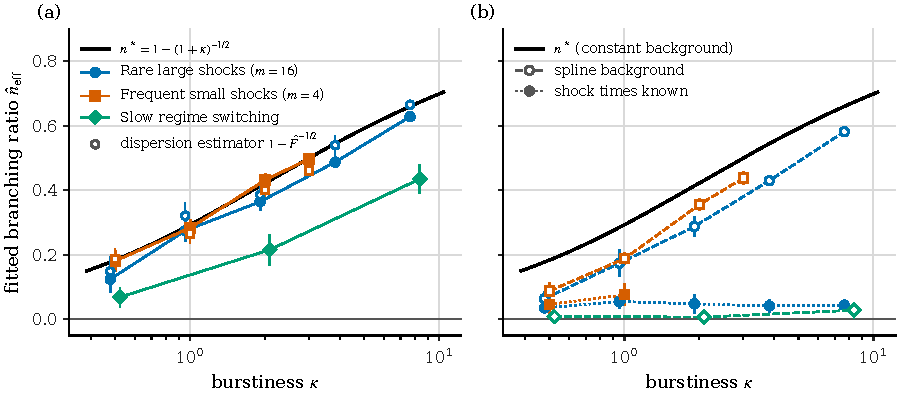
\includegraphics[width=6.0in]{figures/fig-sim-spurious.pdf}
\caption{E2, spurious contagion in synthetic data with \emph{no} contagion ($R=20$ per
point; bars $\pm1.96$ MC SE). (a) $\hat n_{\mathrm{eff}}$ of constant-background fits
against the burstiness $\kappa$ ($T=1000$), with $n^*$ (line), the dispersion estimator
(open markers) and the rare family with $T=10{,}000$ (stars, shifted right). (b) Spline
background (open markers, dashed) and shock times known (filled markers, dotted). Means;
medians are in \cref{tab:sim-e2e3}(a).}
\label{fig:sim-spurious}
\end{figure}

\subsection{E3: thinning and the dark-figure correction}\label{sec:sim-thinning}

\paragraph{Claim} Independent recording with probability $p$ maps $n$ to $n'=h_p(n)$
(\cref{thm:thinning}), and $h_p^{-1}$ undoes the attenuation (\cref{cor:th-darkfig}), with a
floor on its precision set by the uncertainty about $p$. \Cref{thm:thinning}(d) leaves open
whether the maximum likelihood estimator converges to $n'$. Under heterogeneous recording
the homogeneous correction errs as \cref{prop:th-hetthin} predicts.

\paragraph{Design} A univariate exponential Hawkes process with $\beta=1$, $\Lambda=2$,
$T=1500$ and $n\in\{0.3,0.5,0.7\}$ ($R=40$) is thinned at $p\in\{1,0.8,0.6,0.4,0.2\}$, with
nested recorded sets, and refitted. The \emph{naive} estimate is $\hat n'$; the
\emph{corrected} estimate is $h_p^{-1}(\hat n')$ with the delta-method variance
\eqref{eq:th-delta}, with $p$ known or estimated by $\hat p=p(1+rZ)$, $Z\sim N(0,1)$,
clipped to $[0.02,1]$, with standard error $r\hat p$ and relative error
$r\in\{10,30,50\}\%$ (one $Z$ for all three). In the heterogeneous design two equally likely
marks have $n_x=(0.1,0.9)$, so $\bar n=0.5$, and are recorded with
$(p_1,p_2)\in\{(0.2,0.8),(0.5,0.5),(0.8,0.2),(1,1)\}$ ($R=30$).

\paragraph{Results} The maximum likelihood estimate tracks $n'(p)$: over the 15
combinations of $n$ and $p$, $|\text{mean of }\hat n'-n'(p)|\le0.0104$ (MC SE $0.0062$).
Ignoring thinning is not harmless: at $n=0.5$ the naive interval covers the true $n$ in
$0.975$, $0.825$, $0.175$, $0.025$ and $0$ of replicates for $p=1,\dots,0.2$
(\cref{fig:sim-thinning}(a)). The correction with $p$ known has bias between $-0.0004$ and
$-0.0155$ and coverage $0.925$--$1$ at $n=0.5$ and $0.90$--$0.95$ at $n=0.7$, and $10\%$
error in $\hat p$ changes little (\cref{tab:sim-e2e3}(b)). The exception is weak excitation
with heavy thinning: at $n=0.3$ and $p\le0.4$, $n'$ is within a few standard errors of the
boundary (\cref{prop:lrt}(b)), the fitted decay is erratic (means $23.4$ and $110.8$ against
$0.83$ and $0.77$) and coverage falls to $0.85$ and $0.70$; profile-likelihood or bootstrap
intervals are needed there.

Larger errors in $\hat p$ expose the floor of \cref{cor:th-darkfig}. With
$\mathrm{SD}(\hat p)=rp$, the second term of \eqref{eq:th-delta} contributes the standard
deviation $r\,n(1-n)(2-n)/2$, which depends on neither $p$ nor $T$; at $n=0.5$ it is $0.019$,
$0.056$ and $0.094$ for $r=10$, $30$ and $50\%$. Across the five values of $p$ the RMSE of
the corrected estimate is $0.030$--$0.076$ with $10\%$ error, as with $p$ known, but
$0.051$--$0.096$ with $30\%$ and $0.099$--$0.167$ with $50\%$ (\cref{fig:sim-thinning}(c)),
never much below the floor (the lowest values are at $p=1$, where $\hat p$ is clipped).
Uncertainty about coverage, not the number of incidents, then limits precision, and the
delta method understates it: the correction grows faster as $\hat p$ falls than it shrinks
as $\hat p$ rises, so the estimates are skewed upwards (at $n=0.5$ and $r=50\%$, means $0.503$--$0.569$, medians $0.497$--$0.531$), and
coverage falls to $0.875$--$0.975$ for $r=30\%$ and $0.775$--$0.925$ for $r=50\%$ ($n=0.5$).
With coverage estimates this uncertain, $p$ is better propagated by draws.

Under heterogeneous recording the homogeneous correction errs in the direction
\cref{prop:th-hetthin} predicts (\cref{fig:sim-thinning}(d)): its bias relative to $\bar n$
is $+0.0665$, $+0.0273$, $+0.0217$ and $-0.0301$ for positive, zero (equal or complete
recording) and negative $\Cov(p_X,n_X)$, against theoretical $+0.077$, $+0.036$, $+0.036$
and $-0.021$; the fitted $\hat n''$ lies $0.008$--$0.014$ below its second-order value.

\begin{figure}[tbp]
\centering
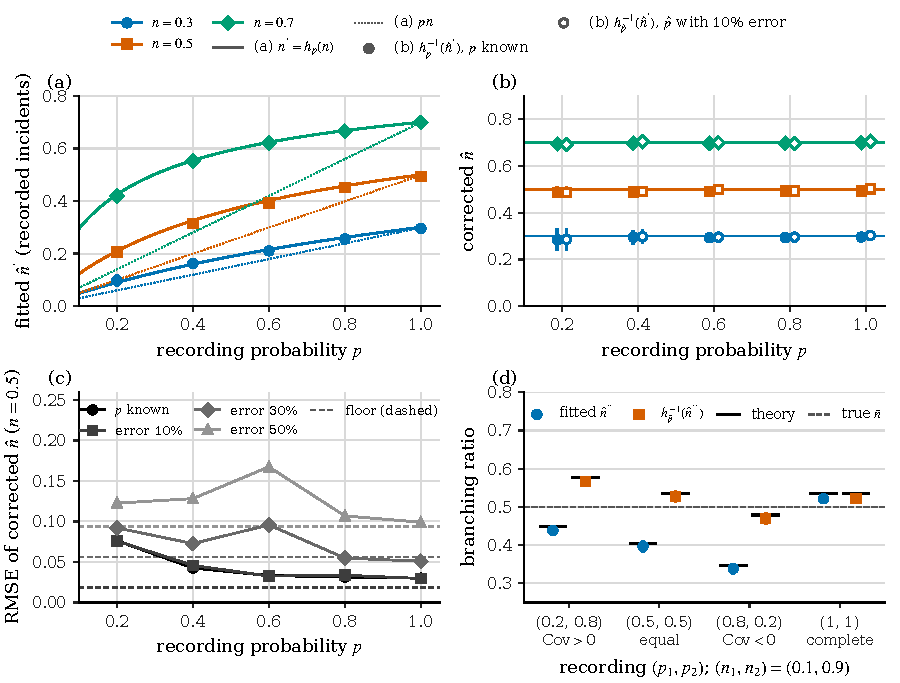
\includegraphics[width=6.0in]{figures/fig-sim-thinning.pdf}
\caption{E3, thinning (synthetic data; bars $\pm1.96$ MC SE). (a) Fitted branching ratio of
the recorded incidents against $p$, with $n'=h_p(n)$ (solid) and $pn$ (dotted); $R=40$. (b)
Corrected estimates with $p$ known (filled) or estimated with $10\%$ error (open); lines mark
the true $n$. (c) The variance floor at $n=0.5$: RMSE of the corrected estimate with $p$
known and with $10$, $30$ and $50\%$ error in $\hat p$, and the floor $r\,n(1-n)(2-n)/2$
(dashed); at $p=1$, $\hat p$ is clipped at $1$. (d) Heterogeneous recording of two marks
with $(n_1,n_2)=(0.1,0.9)$: fitted $\hat n''$ and the homogeneous correction against
\cref{prop:th-hetthin} (solid) and $\bar n=0.5$ (dashed); $R=30$.}
\label{fig:sim-thinning}
\end{figure}

\subsection{E4: the online-to-offline test and common shocks}\label{sec:sim-lrt}

Under $\alpha_{\mathrm{off},\mathrm{on}}=0$ the likelihood-ratio statistic should have the
chi-bar-square limit $\tfrac12\chi^2_0+\tfrac12\chi^2_1$ (\cref{prop:lrt}); an omitted
common shock that reaches online volume first should produce online-to-offline Granger
causality (\cref{rem:th-granger-caveats}(i)), and recording it should remove it
(\cref{cor:equiv-id}(i)). Two streams have
$\Amat=\bigl(\begin{smallmatrix}0.3&\alpha_{\mathrm{off},\mathrm{on}}\\0.2&0.4\end{smallmatrix}\bigr)$
and $T=600$; the shared decay stays identified under $H_0$ (\cref{rem:est-lrt}(i)). Common
shocks arrive at rate $0.05$ and reach the online stream within about half a day, the
offline stream over about four days. The test holds its size (\cref{tab:sim-e4e5}(a) and \cref{fig:sim-lrt}, both in
\cref{app:sim-e1e5}). Under $H_0$ ($R=160$) it rejects in $0.0875$ ($0.022$), $0.0625$
($0.019$) and $0.01875$ ($0.011$) of replicates at the $10$, $5$ and $1\%$ levels, and the
statistic is zero in $0.5625$ ($0.039$) of them; the naive $\chi^2_1$ reference rejects in
$0.025$ at $5\%$. The power is $0.617$, $0.983$ and $1.0$ for
$\alpha_{\mathrm{off},\mathrm{on}}=0.05$, $0.1$ and $0.2$ ($R=60$). With the common shocks
omitted the test rejects in all 60 replicates (mean estimate $0.072$), with no
online-to-offline excitation; with the calendar in the model it rejects in $0.083$
($0.036$), with mean estimate $0.010$. The Davies problem (\cref{sec:est-lrt}) was not
studied (its bootstrap needs about 600 EM fits per dataset); the block tests of the plan
need it, so it must pass the synthetic dry run (\cref{sec:plan-validation}, V4).

\subsection{E6: alerting and nowcasting}\label{sec:sim-alert}

\paragraph{Claim} Thresholding the predictive probability of a surge at $\pi^*$ minimises
the expected cost (\cref{thm:alert}(a)). If the predictive distribution is the conditional
law given the forecaster's information, the randomised PIT is uniform
(\cref{lem:fc-pit}(a)). Reporting delays bias the naive state downward, by the factor
$\E e^{-\beta d}$ under stationarity, and the delay-weighted state is unbiased
(\cref{prop:nowcast}).

\paragraph{Design} Two streams, offline (the target) and online, have
$\Amat=\bigl(\begin{smallmatrix}0.35&0.10\\0.25&0.45\end{smallmatrix}\bigr)$, and external
events arrive as a Poisson process at rate $1/30$ per day with log-normal sizes. Each of 12
replicates has a training period $[0,1000]$ and 150 weekly forecast windows. A surge is a window with at least $c=21$ offline
incidents, the 90th percentile in a separate pilot; the surge rate in the 1800 test windows
is $0.0967$ ($0.0070$). At each origin $t$ the predictive distribution of the offline count
is estimated from 2000 cluster continuations of the state at $t$ (\cref{lem:fc-future}),
with the true parameters or with EM estimates from the training period, in two versions.
One assumes \emph{no future events} after $t$. The other \emph{integrates} over them,
adding to each continuation the clusters of events drawn from the event process for
$(t,t+7]$ (true rate and size law, or those of the training calendar with fitted
loadings); this is the conditional law given the past, to which \cref{lem:fc-pit}(a)
applies (\cref{sec:fc-predictive}). The baselines are a moving-average Poisson forecast (mean of
the last four weekly counts) and climatology. Alerts use $c_{\mathrm{FA}}=1$ and
$c_{\mathrm{miss}}\in\{2,5,10\}$, so $\pi^*\in\{1/3,1/6,1/11\}$. Under delays
(offline only: zero with probability $0.3$, else exponential with mean three days), the
fitted forecast plugs the naive or the Horvitz--Thompson state (\cref{prop:nowcast}(b))
into the continuation. This plug-in is the shortcut that \cref{sec:fc-nowcast} warns is not
the Bayes rule for delayed data; \cref{alg:alert} itself was not run. Surges are defined by
the 90th rather than the plan's 95th percentile, and the baselines are not the plan's
background-only model and persistence rule (\cref{sec:plan-estimands}).

\paragraph{Decisions} The Hawkes rules have the lowest realised cost at every cost ratio
(\cref{tab:sim-e6}, \cref{fig:sim-alert}(a)), for example $0.285$ per window at
$c_{\mathrm{miss}}=5$ with true parameters against $0.451$ for the moving average and
$0.483$ for climatology, which is essentially the best constant rule. The comparison favours
the Hawkes model: the data are generated by it, and the baselines are simple ones, not the
plan's. Fitting the parameters costs almost nothing. Integrating over future events
changes the costs little (paired differences $-0.001$, $-0.002$ and $-0.014$, MC SEs
$0.002$, $0.007$ and $0.016$) but improves the Brier score from $0.0655$ to $0.0628$ (paired
MC SE $0.0006$). It raises the surge probability in every window, trading precision for
recall at $\pi^*=1/6$ ($0.503$ and $0.511$ against $0.614$ and $0.466$).

\paragraph{Calibration} Pooled over all windows, the forecast that integrates over future
events is calibrated (\cref{fig:sim-alert}(d)). With true parameters the PIT gives
$\chi^2=3.3$ on 9 degrees of freedom ($p=0.95$), and the mean forecast exceeds the outcome
by $0.07$ ($0.18$) incidents per window. With fitted parameters $\chi^2=17.1$ ($p=0.048$)
and the bias is $+0.38$ ($0.22$), because the event rate estimated from the training
calendar, $0.0353$ ($0.0018$) on average, exceeds $1/30$. The forecast that assumes no
future events is not calibrated: $\chi^2=175.3$, and it is too low by $1.91$ ($0.18$)
incidents per window with true parameters. That miscalibration comes from a misspecified
forecaster that leaves out the event process, not from the method. What no forecaster can
do is \emph{time} the events. In 108 of the 174 surge windows ($62\%$), an external event
arrives after the forecast origin. Conditionally on whether one arrives, even the
integrating forecast is not calibrated, and cannot be: its PIT values are too low in the
1424 windows without a new event and too high in the 376 with one, $36.4\%$ of them in the
top decile (\cref{fig:sim-alert}(e)). The limitation shows in recall: at $\pi^*=1/6$ the
integrating rule with true parameters detects $89\%$ of the surges in windows without a new
event but $28\%$ of those in windows with one. Alerts should be reissued as soon as a
salient event occurs.

\paragraph{Delays} The naive state is biased downward as \cref{prop:nowcast}(c) predicts:
with true parameters it averages $0.4752$ of the complete-data state, against
$\E e^{-\beta d}=0.475$, and never exceeds it; the Horvitz--Thompson state averages
$1.0033$ of it. In windows without a new event the no-future-event forecast from the naive
state is miscalibrated ($p=0.033$) and that from the nowcast is not ($p=0.435$). Neither
decisions nor pooled calibration show a benefit, however (\cref{tab:sim-e6},
\cref{fig:sim-alert}(b),(f)). With integration the three costs differ by at most $0.012$ at
each ratio, and at $c_{\mathrm{miss}}=5$ the naive state is even slightly cheaper than the
nowcast (paired difference $-0.008$, MC SE $0.003$): its forecasts are lower by $0.42$
incidents per window, which offsets the fitted forecaster's over-forecast. Here the delays
are short and the undelayed online stream carries much of the excitation. The study
confirms the correction of the state, not that the nowcast improves alert decisions.

\begin{table}[tbp]
\centering
\caption{E6, alerting (synthetic data; 12 replicates $\times$ 150 weekly windows). Realised
cost per window at $c_{\mathrm{miss}}/c_{\mathrm{FA}}=2$, $5$ and $10$ (MC SE
$0.008$--$0.06$); precision and recall at $\pi^*=1/6$; Brier score of the surge
probability; pooled PIT statistic $\chi^2_9$ ($5\%$ critical value $16.9$); mean forecast
minus outcome (Bias). ``No future events'': empty calendar after the forecast origin;
``integrating'': future events drawn from the event process. Delayed rows use fitted
parameters; climatology never alerts at $\pi^*=1/6$.}
\label{tab:sim-e6}
\footnotesize
\setlength{\tabcolsep}{4.5pt}
% Generated by code/make_figures.py from results/sim_results.json -- do not edit by hand.
% E6. Cost per window at c_miss/c_FA = 2, 5, 10; precision and recall at c_miss/c_FA = 5;
% Brier score of the surge probability; pooled PIT chi2 (9 df, 1800 windows); mean forecast minus outcome.
\begin{tabular}{@{}lrrrrrrrr@{}}
\toprule
 & \multicolumn{3}{c}{Cost per window} & & & & & \\
\cmidrule(lr){2-4}
Forecaster & 2 & 5 & 10 & Prec. & Recall & Brier & PIT $\chi^2_9$ & Bias \\
\midrule
\multicolumn{9}{@{}l}{\emph{Complete data}} \\
\quad Hawkes, true par., no future events & 0.137 & 0.287 & 0.526 & 0.614 & 0.466 & 0.0655 & 175.3 & $-$1.91 \\
\quad Hawkes, true par., integrating & 0.136 & 0.285 & 0.512 & 0.503 & 0.511 & 0.0628 & 3.3 & $+$0.07 \\
\quad Hawkes, fitted, no future events & 0.137 & 0.287 & 0.534 & 0.594 & 0.471 & 0.0654 & 169.8 & $-$1.75 \\
\quad Hawkes, fitted, integrating & 0.134 & 0.289 & 0.514 & 0.484 & 0.511 & 0.0629 & 17.1 & $+$0.38 \\
\quad Moving-average Poisson & 0.221 & 0.451 & 0.792 & 0.216 & 0.247 & 0.1141 & 1994.3 & $+$0.06 \\
\quad Climatology & 0.193 & 0.483 & 0.898 & --- & 0.000 & 0.0880 & 26.5 & $+$0.94 \\
\addlinespace
\multicolumn{9}{@{}l}{\emph{Reporting delays}} \\
\quad Fitted, naive state, no future events & 0.138 & 0.304 & 0.518 & 0.629 & 0.420 & 0.0668 & 247.8 & $-$2.18 \\
\quad Fitted, HT nowcast, no future events & 0.135 & 0.297 & 0.523 & 0.572 & 0.454 & 0.0654 & 190.5 & $-$1.75 \\
\quad Fitted, naive state, integrating & 0.137 & 0.279 & 0.502 & 0.550 & 0.506 & 0.0633 & 6.8 & $-$0.05 \\
\quad Fitted, HT nowcast, integrating & 0.135 & 0.287 & 0.510 & 0.481 & 0.517 & 0.0630 & 13.3 & $+$0.37 \\
\quad Moving-average Poisson, available counts & 0.226 & 0.478 & 0.848 & 0.177 & 0.161 & 0.1130 & 1879.8 & $-$0.65 \\
\bottomrule
\end{tabular}

\end{table}

\begin{figure}[t]
\centering
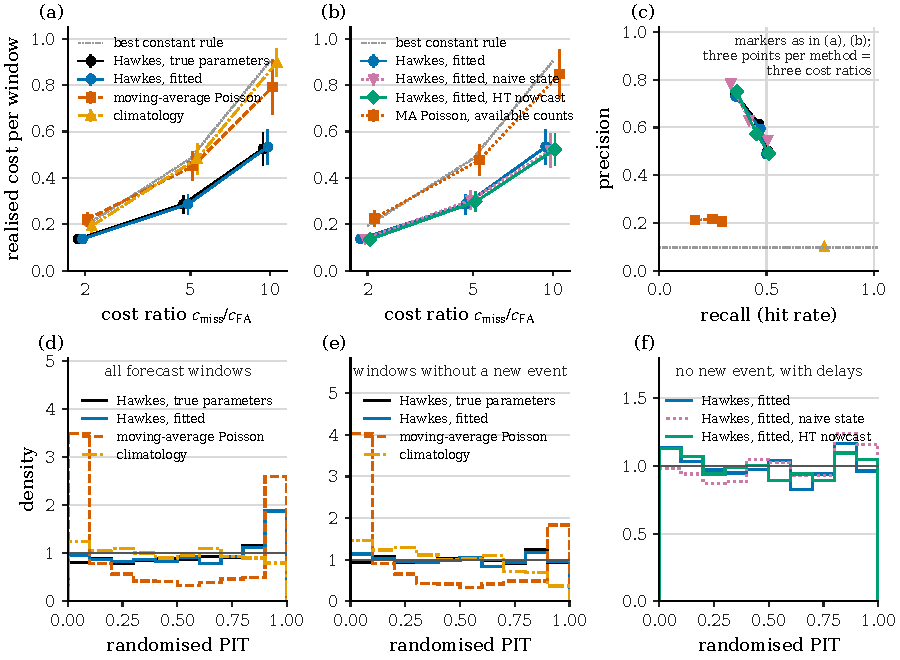
\includegraphics[width=6.0in]{figures/fig-sim-alert.pdf}
\caption{E6, alerting and nowcasting (synthetic data; 12 replicates $\times$ 150 weekly
windows; bars $\pm1.96$ MC SE). Hawkes forecasts with true or fitted parameters, assuming no
future events (dashed, open markers) or integrating over them (solid, filled). (a) Realised
cost per window against the cost ratio; dotted: best constant rule. (b) The same under
reporting delays (fitted, integrating). (c) Precision against recall at the three
thresholds; dotted: surge rate. (d) PIT histograms, all windows. (e) PIT of the integrating
forecast with true parameters, for windows in which an external event arrives after the
origin and for the others. (f) PIT under delays, all windows.}
\label{fig:sim-alert}
\end{figure}

\subsection{What the study does and does not show}\label{sec:sim-limits}

Under the model the tools work as the theory says: EM recovers the branching matrix and
the surge decomposition with close to nominal coverage, the boundary test holds its size,
and the dark-figure correction restores coverage except when excitation is weak and
recording poor, with a floor of about $0.04$--$0.09$ set by a $30$--$50\%$ error in $p$. The
traps are real: a constant background finds contagion where there is none (for rare large
shocks $0.06$--$0.07$ below $n^*$ even with $T=10{,}000$); smoothing does not remove the
artefact of fast shocks, while the shock times largely do, where tested; and an omitted
common shock creates an online-to-offline effect. On Hawkes-generated data a plug-in Hawkes
alert rule beats two simple baselines that are not the plan's. Forecasts that integrate
over future events are calibrated when pooled; no forecaster can time the events, and that
limits recall.

The study has clear limits. Each experiment uses a few parameter points, at most three
streams, exponential kernels and, apart from E2, constant backgrounds; there are no
near-critical systems and no misspecified kernels. The replicate numbers resolve
differences of a few hundredths in branching ratios and about $0.01$--$0.04$ in costs, not
smaller ones. Not evaluated were the Davies sup-test and its bootstraps, Bayesian
estimation and shrinkage, the INAR approximation, nonparametric kernels, the time-rescaling
check, placebo calibration and the imputation algorithm (\cref{alg:alert}); the delay
correction was evaluated only as a plug-in state. Nor did we test whether a flexible
background absorbs genuine contagion, long windows for slow switching, or the selection
rules of the analysis plan. These checks belong to the synthetic dry run of the plan
(\cref{sec:plan-validation}, V4).
}{}
\IfFileExists{sections/09-analysis-plan.tex}{\section{A pre-registered analysis plan}\label{sec:plan}

This section summarises the analysis plan that we intend to register before any outcome
data are examined. \Cref{app:plan} gives it in full, with the replication package and the
timeline. The numerical settings are proposals until registration; later changes will be
reported as deviations. No part of the plan has been carried out on real data. The
simulation study (\cref{sec:simulation}) evaluates EM estimation, surge attribution, the
boundary test, the thinning correction and a plug-in alert, but not the block tests, the
placebo calibration or the selection and decision rules of the plan. These must first pass
a synthetic dry run (V4).

\paragraph{Data and design.} The candidate pilot is the New York City Police Department's
hate-crime file \citep{nypdhate}, restricted to anti-Jewish records from 2019 onwards, with
the five boroughs as offline streams and the final 12 months as a hold-out test period
(\cref{sec:plan-pilot}). The design is chosen on data availability alone. If day-level
occurrence dates can be obtained under a data-use agreement, the model is fitted to them
(Design A). Otherwise it is fitted to record-creation dates as a report-time process, with
an explicit delay distribution and the occurrence month as a constraint (Design B). Online,
ADL and CST streams are conditional on access being confirmed.

\paragraph{Estimands.} (E1) The branching matrix $\Amat$, with $\spr(\Amat)$ and $\Mmat$,
on the recorded scale first and thinning-corrected alongside. (E2) The surge decomposition
$B_k+D_k+C_k$ of \cref{thm:attribution} for every pre-registered event at $H=14$ days, with
$7$ and $28$ days as secondary horizons, and the online-channel share where online streams
are included. (E3) Alert performance with window $\Delta_{\mathrm a}=7$ days against a
background-only model and a persistence rule, at cost ratios agreed with
community-security partners (\cref{sec:plan-estimands}).

\paragraph{Events.} The event list is fixed blind to incident data by the procedure of
\cref{sec:data-events}: classes defined by type, a salience index computed from event data
alone with a threshold that yields 10 to 30 events, independent coding by two coders without
access to incident data, and a hashed freeze before incident data are loaded
(\cref{sec:plan-events}).

\paragraph{Models and tests.} The models are nested: background only (M0), plus shocks
(M1), self-excitation (M2), cross-borough excitation (M3) and online$\leftrightarrow$offline
blocks (M4). Each block of $\Amat$ has one common exponential decay, and the background is a
cubic B-spline with knot spacing $h_b=60$ days plus day-of-week and holiday effects. A step
is taken only if its block test rejects at level $0.05$ and the out-of-sample log score
improves. A block's decay is not identified when all its entries vanish, so each block test
uses the sup-LR statistic \eqref{eq:est-suplr} over nine decays with half-lives from $0.5$
to $21$ days, referred to a parametric bootstrap with $B=499$ replicates from the null fit.
The block tests are applied in a fixed sequence. Entry-level tests within the accepted
blocks form one Holm family at level $0.05$. If the dry run shows a block test to be too
slow or oversized, registered fallbacks apply (\cref{sec:plan-models}).

\paragraph{Sensitivity, validation and decisions.} Eight sensitivity analyses vary the
background flexibility ($h_b\in\{30,60,120,365\}$ days), the recording model, the kernel
family, the delay model, the event list, the spatial resolution, the correction for online
measurement error and the treatment of ties (\cref{sec:plan-sens}). Validation uses
time-rescaling goodness of fit with a bootstrap reference (V1), out-of-sample scores and PIT
histograms (V2), placebo calendars whose dates are drawn from \emph{all} days of the
training period, so that the randomisation hypothesis of \cref{lem:est-placebo} can hold
(V3), and the synthetic dry run (V4) (\cref{sec:plan-validation}). Contagion in a stream is
claimed only if its Holm-adjusted test rejects, its interval excludes zero under the most
flexible background, goodness of fit is not rejected and the placebo false-positive rate is
at most $0.10$. Cross-stream effects are described as Granger-type predictive dependence,
never as causation. Alerts are recommended for operational use only if they beat both
baselines in realised cost (\cref{sec:plan-decisions}).
}{}
\IfFileExists{sections/10-ethics.tex}{\section{Ethics and responsible use}\label{sec:ethics}

Models that forecast surges in hate incidents can protect people. They can
also cause harm through how outputs are worded, where they are shared and
what they are used for. This section sets out the protocol that accompanies
the plan in \cref{sec:plan}. It complements the companion paper's protocol
for victim privacy and record linkage \citep{kornsteinlab2026darkfigure}.

\subsection{Risks of forecasting}\label{sec:ethics-risks}

\paragraph{Stigmatisation.}
A map of elevated predicted intensity can be read as a statement about the
people who live in an area. That reading applies to neighbourhoods where
Jewish residents are targeted, which can come to be seen as ``dangerous''.
It applies equally to any community that observers might wrongly treat as a
source of incidents. The model contains no information about perpetrators,
and its spatial units are recording areas, not communities. Alerts and published maps are therefore
at the borough level or coarser, and never street- or venue-level heat maps.
Finer units used in sensitivity analysis S6 are reported only as summary
statistics. No output ranks neighbourhoods or communities.

\paragraph{Self-fulfilling and self-defeating alerts.}
An alert can change what it predicts. Publicity can raise reporting, which
inflates recorded counts (the time-varying $p_k$ of analysis S2). Protective
deployment can prevent incidents, which makes a correct alert look like a
false alarm. Either effect contaminates prospective evaluation. Alerts
during the prospective period (phase P7) are therefore shared only under the
protocol below, and evaluation reports state which alerts were acted on.

\paragraph{Information hazards.}
Forecasts that name ``hot'' dates or locations could help someone planning
an attack, and could encourage imitation. We therefore publish methods,
code and retrospective results, but no live or near-live forecasts and no
forecast tied to a specific site. Retrospective results are released only
after an embargo (\cref{sec:ethics-disclosure}).

\subsection{Responsible disclosure of alerts}\label{sec:ethics-disclosure}

Alerts produced during the prospective evaluation are handled as follows.
\begin{enumerate}[1.]
  \item \emph{Recipients.} Alerts go only to vetted community-security
  partners, and to a police liaison where the partner agreement provides for
  this. Each partner signs an agreement that limits use to protective
  purposes, such as security staffing and victim support, and excludes
  enforcement targeting of any community.
  \item \emph{Content.} An alert gives the borough or coarser area, the
  window $\Delta$, the predicted probability of exceeding the threshold
  with its uncertainty, and a fixed statement of the model's limitations.
  It contains no individual-level information and no attribution to
  persons, groups or communities.
  \item \emph{Human review.} A named member of the research team reviews
  every alert before release, and may withhold an alert that is plainly
  driven by a data artefact.
  \item \emph{Channel and logging.} Alerts are sent over an encrypted
  channel. Each alert, the decision to release or withhold it, and the
  partner's acknowledgement are logged for audit.
  \item \emph{Embargo.} Alerts are not published. Aggregate evaluation
  results (hit and false-alarm rates by quarter and borough) are published
  no earlier than 90 days after the end of the period they cover.
  \item \emph{Suspension.} Alerts are suspended if rolling calibration
  deteriorates beyond a pre-specified tolerance, or if a partner reports
  misuse.
\end{enumerate}

\subsection{Language and attribution}\label{sec:ethics-language}

The model attributes \emph{timing}, not blame. A positive shock loading
$\beta_k$, or a large direct component $D_k$ after event $e$, means that
recorded incidents in stream $k$ rose after $\tau_e$ by more than the
background and the contagion terms predict. It does not mean that the
parties to the event, the communities associated with them, or the people
who discussed it caused any incident. Incidents are committed by
individual perpetrators, about whom the model contains no information. We
therefore:
\begin{enumerate}[(i)]
  \item describe events as \emph{salient external events} of a stated class
  and date, and do not characterise them politically;
  \item never describe a community, nationality or religious group as a
  source, driver or cause of incidents;
  \item phrase every result in terms of recorded incidents and statistical
  association; this includes the online$\to$offline coefficients, which
  are Granger-type (\cref{prop:granger}); and
  \item report event-level decompositions in an appendix under neutral
  identifiers, with class-level summaries in the main text.
\end{enumerate}

\subsection{Political neutrality}\label{sec:ethics-neutrality}

The paper takes no position on any political conflict, government, movement
or public figure. Neutrality is built into the procedure, not just asserted:
event classes are defined by type and apply to all parties alike
(\cref{sec:plan-events}); the event list is frozen before outcome data are
seen, so events cannot be selected after the fact; every pre-registered
event is reported whatever the result (rule D3); and the event-coding rules
and frozen list are public. Before registration, the event-coding protocol
will be reviewed by at least two external reviewers with differing
perspectives on the events likely to be coded. Their comments and our
responses will be deposited with the registration.

\subsection{Online data}\label{sec:ethics-online}

Online data are used only under the terms of the access route through which
they are obtained, including any conditions on data protection and security
attached to access under Article~40 of the Digital Services Act
\citep{eu2022dsa}. The analysis uses aggregate counts per time bin. We do
not build account-level scores or profiles, do not link online accounts to
offline incidents, victims or suspects, and do not publish post text,
handles or quotations that would allow re-identification. Annotation
samples for estimating classifier error (\cref{eq:data-classerr}) are held
under access control and deleted when the retention period agreed with the
data provider and the ethics board ends. Classifier outputs are used only as
aggregate series. They are never used to flag individuals.

\subsection{Ethics review and data security}\label{sec:ethics-irb}

The protocol, including this section, will be submitted to an institutional
review board or equivalent research ethics committee before any data are
accessed (gate F5). This applies even to publicly downloadable data, because
the plan combines several streams and may involve partner and platform
data. Restricted data are kept on encrypted storage with role-based access,
and use is logged. The custodian who holds the incident data during event
coding (\cref{sec:plan-events}) is separate from the coders. Outputs follow
a minimum-cell rule: counts below 10 are not shown below the borough level,
and any table that could reveal a single incident's date and location is
suppressed or coarsened. Derived counts are released at a resolution no
finer than the source itself publishes; for restricted streams, they are
released weekly or more coarsely. Data are retained no longer than the agreements
allow, and the replication package contains only data whose release is
permitted (\cref{sec:plan-replication}).
}{}
\IfFileExists{sections/11-discussion.tex}{\section{Discussion}\label{sec:discussion}

\paragraph{What the framework makes possible}
After a salient external event, the public argument is usually about whether
the event ``caused'' the surge that followed. The framework replaces that
single question with several that have precise answers under a stated model.
How many incidents in the window would have occurred anyway, how many
responded directly to the event, and how many were set off by other incidents
(\cref{thm:attribution})? How much of that cascade passed through online
streams (\cref{prop:at-channel})? How large is the cascade that one incident
starts in each stream, as measured by the multiplier $\Mmat$? Each answer
comes with an interval and with the assumptions it rests on.

The framework is equally explicit about what the data cannot settle. The
autocorrelation of counts cannot tell contagion from clustered shocks
(\cref{thm:equiv}), and an incomplete event calendar or a rigid background
manufactures contagion (\cref{thm:spurious}). Identification has to come from
outside the counts: from a calendar of events fixed blind to the outcome, from
higher-order information that only the full likelihood exploits, or from
provenance links between incidents (\cref{cor:equiv-id}). The analysis plan
is built around that requirement (\cref{sec:plan-events}). The companion
paper enters at a precise point. Recorded incidents are a thinned version of
all incidents, and thinning attenuates apparent contagion in a known way
(\cref{thm:thinning}). A contagion estimate is therefore only as good as the
coverage estimate behind it, and the uncertainty about coverage sets a floor
under its precision (\cref{cor:th-darkfig}). For those who must act on a
forecast, the alert rule makes the trade-off between false alarms and missed
surges an explicit choice, agreed with the people who bear its costs
(\cref{thm:alert}), and the nowcast keeps reporting delays from hiding a surge
that is already under way (\cref{prop:nowcast}).

\paragraph{Limitations}
We stress six.

\emph{Linearity and the absence of inhibition.} In a linear Hawkes process an
incident can only raise the rate of later incidents. Deterrence, protective
deployment after an alert, arrests and saturation all lower it, and the model
cannot represent them. Where they operate, the fitted excitation is a net
effect, and an alert that prompts successful protection makes itself look
like a false alarm (\cref{sec:ethics-risks}). Nonlinear Hawkes processes,
which allow inhibitory kernels through a link function \citep{bremaud1996},
remove this restriction at the cost of the cluster representation on which
the surge decomposition rests.

\emph{Stationarity and constant parameters.} The theory assumes
$\spr(\Amat)<1$ and parameters that do not change over the study period.
Contagion may itself change, for example after a major event or a shift in
how incidents are publicised, and recording probabilities can move with
attention and with breaks in reporting systems (\cref{sec:data-incidents}).
The change-point monitor of \cref{rem:fc-cusum} can detect such shifts but
does not model them. Estimates close to criticality deserve particular
caution, since a misspecified background pushes the apparent branching ratio
towards one (\cref{rem:th-spurious}).

\emph{Pre-specification of events.} Everything rests on the event calendar.
Events missing from it are absorbed into $\Amat$ (\cref{thm:spurious}). The
salience index and its threshold are choices, and the sensitivity analysis can
vary them but not remove them (\cref{sec:plan-sens}). More fundamentally, the
shock term treats event times as exogenous. Some candidate events, such as
public statements, may themselves respond to a wave of incidents. Such
reverse dependence violates the model, and blind coding of the calendar does
not prevent it.

\emph{Classifier error in online streams.} An online stream is the output of
a classifier applied to a defined corpus. It measures that corpus, not
platform-wide prevalence, and its error rates may change after salient events
precisely when they matter most (\cref{eq:data-classerr}). Independent errors
cannot create online-to-offline Granger causality under the null, but they
dilute it under the alternative, and errors that move with common shocks can
mimic it (\cref{rem:th-granger-caveats}). Every online-to-offline coefficient
is a statement about predictive dependence between measured series, not about
the influence of online speech on offline behaviour.

\emph{Ecological interpretation.} The streams are aggregates over recording
areas and offence categories. A coefficient $\alpha_{kj}$ summarises how the
counts of two streams move together in time. It does not say who influenced
whom, and it says nothing about the people who live in a region. The
mechanisms that could produce self-excitation (imitation, emboldenment,
diffusion through networks, repeat targeting) are hypotheses that the model
does not separate (\cref{sec:th-meaning}). Family trees reconstructed by EM
are probabilistic summaries under the model, not findings about individual
incidents.

\emph{Independent recording.} The thinning results assume that each incident
is recorded independently of the history. If salient events raise the
propensity to report, or if severe incidents are both more productive and
more often recorded, the correction can err in either direction
(\cref{prop:th-hetthin}). The plan treats these departures as sensitivity
analyses, not as solved problems.

\paragraph{Extensions}
Four extensions seem most valuable. First, \emph{spatio-temporal kernels} of
the epidemic-type aftershock (ETAS) kind \citep{ogata1988,mohler2011} would
replace a fixed partition into regions by a kernel in space and time
\citep{reinhart2018}. Their outputs would have to respect the ethics protocol,
which rules out street- or venue-level maps (\cref{sec:ethics-risks}). Second,
\emph{marked and typed incidents}: letting the productivity of an incident
depend on its offence type, severity or target addresses the bias of
\cref{prop:th-hetthin} directly, and with many streams, sparse or low-rank
estimates of $\Amat$ \citep{zhou2013,hansen2015} become essential. Third,
\emph{nonlinear Hawkes processes} with inhibitory kernels
\citep{bremaud1996}, whose Granger-causal graphs remain available
\citep{eichler2017}, would let deterrence and protection enter the model
rather than its residuals. Fourth, and closest to this series, \emph{joint
estimation with the dark-figure model}. Here the recording probability enters
as a plug-in from the companion paper. A joint model would treat each list as
a delayed, time-varying thinning of one latent self-exciting process, so that
linked records from several lists inform both the dark figure and the
dynamics. The companion paper names continuous-time, open-population
estimation as its own leading extension \citep{kornsteinlab2026darkfigure};
the framework developed here supplies the point process it needs.

\paragraph{Why model the dynamics}
A count says how many incidents were recorded. It does not say where they
came from. A surge that is mostly a direct reaction to an event calls for
vigilance in the days after similar events. A surge sustained by contagion
calls for breaking the chain early, because every incident prevented also
prevents the incidents it would have triggered. A surge that travels from
online to offline calls for watching the online streams. These are different
claims about how hostility spreads, and they carry different
responsibilities. The data can support some of these claims, and on some
questions they cannot decide between rival explanations. Stating which is
which, with assumptions in the open and a plan fixed before the data are
seen, is how a measurement programme can take seriously both the people who
live through a surge and the evidence about it.
}{}

% ======================= declarations =======================
\section*{Declarations}
\paragraph{Funding} None.
\paragraph{Competing interests} None declared.
\paragraph{AI assistance} This paper was drafted with substantial assistance
from AI language models (Anthropic's Claude), directed and reviewed by the
Kornstein Lab; all derivations were checked numerically and by independent
automated review, and all simulation numbers are produced by the released
code.
\paragraph{Code and data availability} The code for the simulation study (the
\texttt{hawkes} Python package, the experiment driver
\texttt{run\_experiments.py} with its deterministic seeds, and the script that
produces every figure and table of \cref{sec:simulation}) is in the paper's
repository, together with the simulation output (\cref{app:sim-repro}). All
data in this paper are synthetic and are regenerated by that code. No real
incident data were used.

\bibliographystyle{plainnat}
\bibliography{refs,bib/sources,bib/theory,bib/attribution,bib/estimation,bib/lead}

\clearpage
\appendix
\IfFileExists{appendix/A1-identification-proofs.tex}{\section{Proofs for Section~\ref{sec:identification}}\label{app:idproofs}

Throughout, a stationary $M$-variate point process $\bm N$ with mean
$\bar{\bm\Lambda}$ has a covariance measure
$\operatorname{diag}(\bar{\bm\Lambda})\delta_0(\dd u)+\bm c(u)\,\dd u$, and Bartlett
spectrum \eqref{eq:th-bartlett-def}. All Bartlett spectra below have continuous
densities. Equality of spectra therefore means equality of these densities at every
$\omega$.

\subsection{Auxiliary lemmas}\label{app:th-lemmas}

\begin{lemma}[Cox processes and independent thinning]\label{lem:th-cox2}
\begin{enumerate}[(a)]
  \item Let $\bm N$ be an $M$-variate stationary Cox process directed by
  $\bm\xi=(\xi_k)$. Assume $\E\xi_k(0)^2<\infty$, write $\bar{\bm\Lambda}$ for the mean
  and $\bm c_\xi(u)=\Cov\{\bm\xi(t+u),\bm\xi(t)\}$ for the covariance, and assume
  $\bm c_\xi$ has integrable entries. Then $\bm N$ has covariance density $\bm c_\xi$
  and Bartlett spectrum
  $(2\pi)^{-1}[\operatorname{diag}(\bar{\bm\Lambda})+\hat{\bm c}_\xi(\omega)]$, where
  $\hat{\bm c}_\xi(\omega)$ is Hermitian and positive semidefinite for every $\omega$.
  \item Let $\bm N$ be stationary with mean $\bar{\bm\Lambda}$ and covariance density
  $\bm c$. Record each point of stream $k$ independently with probability $p_k$, and
  let $\bm P=\operatorname{diag}(p_k)$. The recorded process $\bm N^{\bm P}$ has mean
  $\bm P\bar{\bm\Lambda}$ and covariance density $\bm P\bm c(u)\bm P$.
\end{enumerate}
\end{lemma}

\begin{proof}
(a) Given $\bm\xi$, the streams are independent Poisson processes. Hence, for bounded
Borel sets $I,J$,
\[
\E[N_k(I)N_j(J)\mid\bm\xi]=\delta_{kj}\int_{I\cap J}\xi_k
+\int_I\xi_k\int_J\xi_j .
\]
Taking expectations gives
$\Cov\{N_k(I),N_j(J)\}=\delta_{kj}\bar\Lambda_k|I\cap J|+\int_I\int_J c_{\xi,kj}(t-s)\,\dd t\,\dd s$.
For $\bm w\in\mathbb C^M$, the function $\bm w^*\bm c_\xi(u)\bm w$ is the covariance
function of the stationary process $\bm w^*\bm\xi$. It is integrable, so by Fej\'er's
theorem its Fourier transform is
\[
\lim_{T\to\infty}T^{-1}\,\E\Big|\int_0^Te^{-i\omega t}\{\bm w^*\bm\xi(t)-\E\bm w^*\bm\xi(t)\}\,\dd t\Big|^2\ge0 .
\]

(b) Let $R_i$ be the recording indicators. Pairs of distinct points contribute
$\E[R_iR_{i'}]=p_kp_j$ times the second factorial moment measure, whose density off the
diagonal is $\bar\Lambda_k\bar\Lambda_j+c_{kj}$. Each point paired with itself
contributes $p_k\bar\Lambda_k|I\cap J|$ when $k=j$. Subtracting
$p_kp_j\bar\Lambda_k\bar\Lambda_j|I||J|$ gives the claim.
\end{proof}

\begin{lemma}[Poisson cluster processes]\label{lem:th-cluster}
Let $N$ be a stationary Poisson cluster process on $\mathbb R$. Cluster centres form a
Poisson process of rate $r$. Each centre $x$ carries an independent copy of a finite
random configuration $\{y_1,\dots,y_{\mathcal S}\}$, possibly empty, placed at $x+y_i$. Assume
$\E e^{u_0\mathcal S}<\infty$ for some $u_0>0$. Then:
\begin{enumerate}[(a)]
  \item for every $j\ge1$,
  $\chi_j=\lim_{T\to\infty}T^{-1}\operatorname{cum}_jN(0,T]=r\,\E \mathcal S^j$;
  \item the law of $N$ determines $w(k)=r\Pr(\mathcal S=k)$ for every $k\ge1$.
\end{enumerate}
\end{lemma}

\begin{proof}
(a) Let $Y(x)$ be the number of points of a cluster centred at $x$ that fall in
$(0,T]$. The marked Poisson process of centres has Laplace functional
\[
\log\E e^{-sN(0,T]}=-r\int_{\mathbb R}\E[1-e^{-sY(x)}]\,\dd x,\qquad s\ge0 .
\]
For every cluster, $Y(x)^j\le \mathcal S^{j-1}Y(x)$ and $\int Y(x)\,\dd x=\mathcal S\,T$. Hence
$\int\E Y(x)^j\,\dd x\le T\,\E \mathcal S^j<\infty$. By dominated convergence, the right-hand
side is $j$ times differentiable at $s=0+$, with $j$th derivative
$(-1)^jr\int\E Y(x)^j\,\dd x$. Therefore $\E N(0,T]^j<\infty$ by monotone convergence,
and
\[
\operatorname{cum}_jN(0,T]=r\int_{\mathbb R}\E Y(x)^j\,\dd x .
\]
Let $\operatorname{diam}=\max_iy_i-\min_iy_i$. Then $Y(x)=\mathcal S$ on an interval of
$x$-values of length $(T-\operatorname{diam})_+$, so
\[
\mathcal S^j(1-\operatorname{diam}/T)_+\le T^{-1}\int Y(x)^j\,\dd x\le \mathcal S^j .
\]
Dominated convergence gives $T^{-1}\operatorname{cum}_jN(0,T]\to r\E \mathcal S^j$.

(b) Suppose two such processes have the same law. By (a), $r\E \mathcal S^j=r'\E \mathcal S'^j$ for every
$j\ge1$. The finite measures $\nu(k)=k\,w(k)$ and $\nu'(k)=k\,w'(k)$ on
$\{1,2,\dots\}$ then have the same moments of every order $j\ge0$. Both have finite
exponential moments for $u<u_0$. Their generating functions
$\sum_k\nu(k)z^k$ are therefore analytic for $|z|<e^{u_0}$ and agree, so
$\nu=\nu'$ and hence $w=w'$.
\end{proof}

By \cref{prop:stationary}, a stationary Hawkes process with any kernel satisfies
\cref{lem:th-cluster} with $r=\mu$ and $\mathcal S\sim$ Borel$(n)$. The process
$C(\nu,r,a,\gamma)$ superposes a Poisson process of rate $\nu$ (clusters of size $1$)
and a Neyman--Scott process with centre rate $r$ and $\mathcal S\sim\Pois(m)$. It therefore satisfies
the lemma with $w_C(k)=\nu\ind{k=1}+r e^{-m}m^k/k!$. Independent $p$-thinning of a
Poisson cluster process gives a Poisson cluster process with cluster size
$\Bin(\mathcal S,p)$.

\begin{lemma}[Janossy densities identify the intensity]\label{lem:th-janossy}
Let $\bm N$ be an $M$-variate point process on $[0,T]$ with $\E\bm N[0,T]<\infty$. Its
intensity, with respect to its own history and a deterministic calendar, is
$\lambda_k(t)=h_k(t;\bm N|_{[0,t)})$ for measurable functionals with
$h_k\ge h_{\min}>0$. For a configuration $x$ on $[0,t]$ with points
$(s_1,k_1),\dots,(s_m,k_m)$, $s_1<\dots<s_m$, the Janossy density of
$\bm N|_{[0,t]}$ is
\[
j_t(x)=\prod_{i=1}^m h_{k_i}(s_i;x_{<s_i})\exp\Big\{-\sum_k\int_0^t h_k(u;x_{<u})\,\dd u\Big\}>0
\]
\citep[Ch.~7]{daley2003}. For a configuration $x$ on $[0,t)$,
$h_k(t;x)=j_t(x\cup\{(t,k)\})/j_t(x)$. Consequently, if two such specifications
$h^{(1)},h^{(2)}$ give the same law on $[0,T]$, then
$h^{(1)}_k(t;x)=h^{(2)}_k(t;x)$ for almost every $(t,x)$ with respect to Lebesgue
measure times the Lebesgue--Poisson measure. In particular this holds for almost every
$t$ at $x=\emptyset$, and for almost every $(s,t)$ at $x=\{(s,j)\}$.
\end{lemma}

\begin{proof}
Adding a point at the right end $t$ multiplies $j_t$ by $h_k(t;x)$ and leaves the
integral unchanged, which gives the ratio formula. The law determines its Janossy
densities up to null sets. Since $j_t>0$, almost-everywhere statements under the law
transfer to the Lebesgue--Poisson reference measure. The empty configuration is an atom
of that measure, and the one-point configurations carry the measure $\dd s$.
\end{proof}

\begin{lemma}[Affine observable intensity characterises the Hawkes law]\label{lem:th-affine}
Let $H=H(\mu,\varphi)$ be a stationary Hawkes process with kernel
$\varphi\in L^1\cap L^2$, $\int\varphi=n<1$. Let $N$ be a stationary point process,
second-order equivalent to $H$, whose intensity with respect to its own history is
$\lambda(t)=c+\int_{(-\infty,t)}h(t-s)\,\dN(s)$, with $c>0$, $h\ge0$,
$h\in L^1\cap L^2$ and $\int h<1$. Then $h=\varphi$ almost everywhere, $c=\mu$, and
$\Pr_N=\Pr_H$.
\end{lemma}

\begin{proof}
Let $c_N$ be the covariance density of $N$. Since $\dN(t)-\lambda(t)\dd t$ is
orthogonal to $\Hist_{t-}$, we have $\Cov\{\dN(t)-\lambda(t)\dd t,\dN(s)\}=0$ for
$s<t$. Expanding $\Cov\{\lambda(t),\dN(s)\}$ gives, for $u>0$,
\begin{equation}\label{eq:th-wh}
c_N(u)=\bar\Lambda h(u)+\int_0^\infty h(v)\,c_N(u-v)\,\dd v .
\end{equation}
The kernel $\varphi$ solves \eqref{eq:th-wh} with the same $c_N=c_H$, since $H$ has
affine intensity with kernel $\varphi$. The difference $d=h-\varphi\in L^1\cap L^2$ is
supported on $(0,\infty)$ and satisfies
$\bar\Lambda d(u)+\int_0^\infty d(v)c_N(u-v)\,\dd v=0$ for $u>0$. Multiply by $d(u)$,
integrate over $u>0$ and apply Parseval:
\[
0=\frac1{2\pi}\int|\hat d(\omega)|^2\{\bar\Lambda+\hat c_N(\omega)\}\,\dd\omega
=\int|\hat d(\omega)|^2f_H(\omega)\,\dd\omega .
\]
Since $|1-\hat\varphi|\le1+n$, we have $f_H\ge\bar\Lambda(1+n)^{-2}/(2\pi)>0$. Hence
$\hat d=0$, and so $d=0$. Taking expectations of the intensity gives
$c=\bar\Lambda(1-n)=\mu$. Thus $N$ is a stationary solution of the Hawkes equation with
parameters $(\mu,\varphi)$, and $\Pr_N=\Pr_H$ by the uniqueness result of
\citet{bremaud1996}.
\end{proof}

\subsection{Proof of \texorpdfstring{\cref{thm:equiv}}{Theorem (equivalence)}}

(a) By \eqref{eq:th-fH} and \eqref{eq:th-fC}, the means are $\bar\Lambda$ and
$\nu+r a/\gamma$. Given equal means, the spectra agree if and only if
\[
\frac{\bar\Lambda\beta^2n(2-n)}{\beta^2(1-n)^2+x}=\frac{r a^2}{\gamma^2+x}
\qquad\text{for all }x=\omega^2\ge0 .
\]
Both numerators are positive. Cross-multiplying and comparing coefficients in $x$
gives $r a^2=\bar\Lambda\beta^2n(2-n)$ and $\gamma^2=\beta^2(1-n)^2$. The converse is
immediate.

(b) Solving \eqref{eq:th-match} for given $a$ gives
$r=\bar\Lambda\beta^2n(2-n)/a^2$ and
\[
\nu=\bar\Lambda-\frac{r a}{\gamma}
=\bar\Lambda\Big(1-\frac{\beta n(2-n)}{a(1-n)}\Big),
\]
which is nonnegative if and only if $a\ge a_{\min}$. With $m=a/\gamma$,
$m_{\min}=a_{\min}/\{\beta(1-n)\}=n(2-n)/(1-n)^2$, which equals $F_\infty-1$ by
\cref{prop:th-spectrum}. Also $r m^2=r a^2/\gamma^2=\bar\Lambda n(2-n)/(1-n)^2$.

(c) For bins $I,J$, $\Cov\{N(I),N(J)\}$ integrates the covariance measure, which is
the inverse Fourier transform of the Bartlett spectrum. The variance-time curve
$\Var N(0,w]=\bar\Lambda w+2\int_0^w(w-u)c(u)\,\dd u$, the index of dispersion and the
expected periodogram are functionals of the same objects. Both $H$ and $C$ are
stationary Poisson cluster processes with almost surely finite clusters, so they are
mixing \citep[Ch.~12]{daley2008}. Their binned count sequences are therefore stationary
and ergodic, with finite second moments. By Birkhoff's theorem, empirical means and
autocovariances converge almost surely to the common population values. The
continuous mapping theorem concludes the proof. \qed

\subsection{Proof of \texorpdfstring{\cref{prop:th-cm}}{Proposition (CM kernels)}}

\emph{Step 1: finite mixtures.} Let $\varphi(t)=\sum_{i=1}^Kc_ie^{-b_it}$ with
$0<b_1<\dots<b_K$, $c_i>0$ and $\sum_ic_i/b_i=n<1$. Its Laplace transform
$\tilde\varphi(z)=\sum_ic_i/(z+b_i)$ is strictly decreasing on each interval between
consecutive poles. On $(-b_1,\infty)$ it falls from $+\infty$ to $0$ and equals $n<1$
at $z=0$. Hence $\tilde\varphi=1$ at exactly one point $z_1\in(-b_1,0)$. On each
$(-b_{i+1},-b_i)$ it falls from $+\infty$ to $-\infty$, which gives one more root
$z_{i+1}$.

Write $1-\tilde\varphi=P_1/P_0$ with $P_0(z)=\prod_i(z+b_i)$, so that $P_1$ is monic of
degree $K$. These $K$ roots are then all the roots of $P_1$; they are real, negative and simple.
Moreover $P_0-P_1$ has degree $K-1$, so
\[
\tilde R=\frac{\tilde\varphi}{1-\tilde\varphi}=\frac{P_0-P_1}{P_1}
=\sum_{l=1}^K\frac{\upsilon_l}{z-z_l},\qquad
\upsilon_l=\frac{1}{-\tilde\varphi'(z_l)}>0,
\]
since $\tilde\varphi(z_l)=1$ and $\tilde\varphi'<0$. The function
$\sum_l\upsilon_le^{z_lt}$ and the resolvent $R=\sum_j\varphi^{*j}\in L^1$ have the same
Laplace transform on $z\ge0$. Hence $R(t)=\sum_l\upsilon_le^{z_lt}$, a positive combination of
decaying exponentials, which is completely monotone. Also
$R(0+)=\lim_{z\to\infty}z\tilde R(z)=\varphi(0+)$.

\emph{Step 2: general completely monotone kernels.} By Bernstein's theorem,
$\varphi(t)=n\int_{(0,\infty)}e^{-bt}\sigma(\dd b)$ with $\int\sigma(\dd b)/b=1$. Fix
$\iota\ge1$ and partition $(2^{-\iota},2^\iota]$ into cells of width $2^{-\iota}$. Let
\[
\varphi_\iota(t)=n\sum_I\sigma(I)e^{-b_I^+t},
\]
where $b_I^+$ is the right end of cell $I$. Each $\varphi_\iota$ is a finite exponential
mixture. Refining a cell or extending the range can only increase $\varphi_\iota$, so
$\varphi_\iota\le\varphi_{\iota+1}\le\varphi$, and $\varphi_\iota\uparrow\varphi$ pointwise by
monotone convergence. Hence $\int\varphi_\iota\le n<1$ and, by Step 1, each
$R_\iota=\sum_k\varphi_\iota^{*k}$ is completely monotone.

Convolution powers are monotone in the kernel, so $R_\iota\uparrow R$ pointwise by monotone
convergence. The limit $R$ is nonincreasing and integrable, with $\int R=n/(1-n)$, so it
is finite on $(0,\infty)$. A pointwise limit of completely monotone functions is
completely monotone \citep[Cor.~1.6]{schilling2012}. Moreover
\[
R(0+)=\sup_{\iota}R_\iota(0+)=\sup_{\iota}\varphi_\iota(0+)\le\varphi(0+)<\infty .
\]

\emph{Step 3: covariance.} By \cref{prop:th-spectrum},
$2\pi f_H=\bar\Lambda|1+\hat R|^2$, so for $u\ne0$
\[
c_H(u)=\bar\Lambda\Big[R(|u|)+\int_0^\infty R(v)R(v+|u|)\,\dd v\Big].
\]
Write $R(t)=\int e^{-bt}\varpi(\dd b)$. By Tonelli,
$\int_0^\infty R(v)R(v+u)\,\dd v=\iint e^{-b'u}(b+b')^{-1}\varpi(\dd b)\varpi(\dd b')$.
Hence $c_H(u)=\int e^{-b|u|}\mathcal K(\dd b)$ with
\[
\mathcal K(\dd b)=\bar\Lambda\Big[1+\int\frac{\varpi(\dd b')}{b+b'}\Big]\varpi(\dd b)\ge0 .
\]
If $\varpi$ has $K$ atoms, so does $\mathcal K$. Also
$Z=\int \mathcal K(\dd b)/b=\tfrac12\int_{\mathbb R}c_H=\tfrac12\{2\pi f_H(0)-\bar\Lambda\}=\bar\Lambda(F_\infty-1)/2$,
and $\int \mathcal K(\dd b)=c_H(0)<\infty$ by Step 2.

\emph{Step 4: a Cox process with the same second-order structure.} Each shot integrates
to $m$, so $\E\xi=\nu+r m=\bar\Lambda$. By Campbell's theorem for the marked Poisson
process $\{(c_\ell,\Gamma_\ell)\}$, for $u\ge0$,
\[
\Cov\{\xi(t),\xi(t+u)\}=r\,\E\int_{-\infty}^tm^2\Gamma^2e^{-\Gamma(t-c)}e^{-\Gamma(t+u-c)}\,\dd c
=\frac{r m^2}{2}\int b\,e^{-bu}\,\pi(\dd b)=\frac{r m^2}{2Z}\int e^{-bu}\mathcal K(\dd b),
\]
which equals $c_H(u)$ for $r=2Z/m^2$. Then
$\nu=\bar\Lambda-2Z/m=\bar\Lambda\{1-(F_\infty-1)/m\}\ge0$ if and only if
$m\ge F_\infty-1$. Also $\E\xi^2<\infty$ because $c_H(0)<\infty$. By
\cref{lem:th-cox2}(a), the Cox process has mean $\bar\Lambda$ and covariance density
$c_H$, so it is second-order equivalent to $H$.

\emph{Step 5.} $2\pi f_H(\omega)=\bar\Lambda+\int2b(b^2+\omega^2)^{-1}\mathcal K(\dd b)\ge\bar\Lambda$.

\emph{Gamma kernel (\cref{rem:th-noncm}).} For $g(t)=\beta^2te^{-\beta t}$, put
$x=\omega^2/\beta^2$. Then
\[
|1-\hat\varphi|^2=\frac{(1-n-x)^2+4x}{(1+x)^2}.
\]
Its derivative in $x$ has the sign of $3-n-x$, so it is maximised at $x=3-n$, where it
equals $4/(4-n)$. Hence $\min_\omega2\pi f_H/\bar\Lambda=1-n/4$. \qed

\subsection{Proof of \texorpdfstring{\cref{prop:th-mv}}{Proposition (multivariate)}}

(a) This is \cref{lem:th-cox2}(a).

(b) Row $k$ of $\Imat-\hat\Phik$ is $\bm e_k^{\top}$, so
$\bm e_k^{\top}=\bm e_k^{\top}\bm G$. Hence $(\bm G\bm\Delta\bm G^*)_{kk}=\bar\Lambda_k$ and
$(\bm G\bm\Delta\bm G^*)_{jk}=G_{jk}\bar\Lambda_k$, where
$\bm\Delta=\operatorname{diag}(\bar{\bm\Lambda})$. Thus $E_{H,kk}\equiv0$ and
$E_{H,jk}=G_{jk}\bar\Lambda_k$. At $\omega=0$,
$\bm G(0)=\Mmat=\sum_m\Amat^m\ge\Amat$ entrywise, so $G_{jk}(0)\ge\alpha_{jk}>0$.
Since $\hat\Phik$ is continuous, $G_{jk}\neq0$ on a neighbourhood $U$ of $0$. On $U$,
the principal $2\times2$ submatrix of $\bm E_H$ indexed by $\{k,j\}$ has determinant
$-|E_{H,jk}|^2<0$, so $\bm E_H$ is not positive semidefinite there. By (a), no Cox
process has this spectrum.

(c) Campbell's theorem gives
$\Cov\{\xi_k(t+u),\xi_j(t)\}=r\E[a_ka_j]\int s_k(t+u-c)s_j(t-c)\,\dd c$. \qed

\subsection{Proof of \texorpdfstring{\cref{thm:spurious}}{Theorem (spurious contagion)}}

(a) By \cref{lem:th-cox2}, $2\pi f_N(\omega)=\bar\Lambda+2\sigma^2\gamma/(\gamma^2+\omega^2)$.
An exponential Hawkes process has
$2\pi f(\omega)=\bar\Lambda_H+\bar\Lambda_H\beta^2n(2-n)/\{\beta^2(1-n)^2+\omega^2\}$.
As in the proof of \cref{thm:equiv}(a), second-order equivalence holds if and only if
$\bar\Lambda_H=\bar\Lambda$, $\beta(1-n)=\gamma$ and
$\bar\Lambda\beta^2n(2-n)=2\sigma^2\gamma$. Using
$\beta^2n(2-n)=\gamma^2\{(1-n)^{-2}-1\}$, the last condition becomes
\[
(1-n)^{-2}=1+2\sigma^2/(\bar\Lambda\gamma)=1+\kappa ,
\]
since $\int c_\xi=2\sigma^2/\gamma$. This has the unique solution $n^*\in(0,1)$, and
then $\beta^*=\gamma/(1-n^*)$ and $\mu^*=\bar\Lambda(1-n^*)$. For the shot-noise process,
$\sigma^2=r a^2/(2\gamma)$. For the two-state chain,
$\Pr(X_u=1\mid X_0=1)=\pi_1+\pi_0e^{-(q_{01}+q_{10})u}$, which gives
$c_\xi(u)=(\lambda_1-\lambda_0)^2\pi_0\pi_1e^{-(q_{01}+q_{10})|u|}$.

(b) Let $\bm m(\vartheta)$ denote the population counterpart of $\hat{\bm m}_T$. Since $N$
is stationary and ergodic with finite second moments, $\hat{\bm m}_T\to\bm m(\vartheta^*)$
almost surely under $N$, by Birkhoff's theorem and (a). Under $H(\vartheta^*)$, which is
ergodic (proof of \cref{thm:equiv}(c)), also $\hat{\bm m}_T\to\bm m(\vartheta^*)$, and by
assumption $G(\hat{\bm m}_T)\to\vartheta^*$. Continuity of $G$ then forces
$G(\bm m(\vartheta^*))=\vartheta^*$. Hence, under $N$,
$\hat\vartheta_T=G(\hat{\bm m}_T)\to G(\bm m(\vartheta^*))=\vartheta^*$.

(c) $\hat c_\xi$ is continuous because $c_\xi\in L^1$, so
$F_\infty(N)=1+\hat c_\xi(0)/\bar\Lambda=1+\kappa$. For a Hawkes process,
$F_\infty=|1-\hat\varphi(0)|^{-2}=(1-n)^{-2}$, so $n_F=n$.

(d) Fix $\beta$ and set $X(t)=\int_{(-\infty,t)}g_\beta(t-s)\,\dN(s)\ge0$, a predictable
stationary process with $\E X=\bar\Lambda$. The second factorial moment measure of $N$
has density $\bar\Lambda^2+c(t-s)$ off the diagonal, so
\begin{equation}\label{eq:th-EXdN}
\E\int_0^1X(t)\,\dN(t)=\int_0^1\int_{-\infty}^{t}g_\beta(t-s)\{\bar\Lambda^2+c(t-s)\}\,\dd s\,\dd t
=\bar\Lambda^2+I_\beta,
\qquad I_\beta=\int_0^\infty g_\beta c .
\end{equation}
Since $\log\mu\le\log\lambda_\vartheta\le\log\mu+nX/\mu$, the function $L$ is finite.

For $n=0$, $L(\mu,0,\beta)=\bar\Lambda\log\mu-\mu$, which is uniquely maximised at
$\mu=\bar\Lambda$ with value $\bar\Lambda\log\bar\Lambda-\bar\Lambda$. Now fix
$\mu=\bar\Lambda$ and $\beta=\beta_0$. By concavity, the difference quotients
$D_n=\{\log(\bar\Lambda+nX)-\log\bar\Lambda\}/n\ge0$ increase to $X/\bar\Lambda$ as
$n\downarrow0$. By monotone convergence and \eqref{eq:th-EXdN},
\[
\frac{L(\bar\Lambda,n,\beta_0)-L(\bar\Lambda,0,\beta_0)}{n}
=\E\int_0^1D_n\,\dN-\bar\Lambda\ \longrightarrow\ \frac{I_{\beta_0}}{\bar\Lambda}>0 .
\]
Hence $L(\bar\Lambda,n,\beta_0)>\bar\Lambda\log\bar\Lambda-\bar\Lambda$ for all small
$n>0$. For $C$, $c(u)=\{r a^2/(2\gamma)\}e^{-\gamma|u|}$, and integrating against
$\beta e^{-\beta u}$ gives the stated $I_\beta$. \qed

\subsection{Proof of \texorpdfstring{\cref{cor:equiv-id}}{Corollary (identification)}}

(i) Under \cref{ass:th-model} the Volterra resolvent of $\Phik$ on $[0,T]$ is
integrable, so $\E\bm N[0,T]<\infty$, and the intensity has the form of
\cref{lem:th-janossy} with
\[
h_k(t;x)=m_k(t)+\sum_j\sum_{s\in x_j}\varphi_{kj}(t-s),\qquad h_k\ge\inf\mu_k>0 .
\]
Take two parameter values with the same law. Taking $x=\emptyset$ in
\cref{lem:th-janossy} gives $m^{(1)}_k=m^{(2)}_k$ almost everywhere on $[0,T]$. Taking
$x=\{(s,j)\}$ then gives $\varphi^{(1)}_{kj}(t-s)=\varphi^{(2)}_{kj}(t-s)$ for almost
every $0<s<t<T$. By Fubini, $\varphi^{(1)}_{kj}=\varphi^{(2)}_{kj}$ almost everywhere
on $(0,T)$.

For the sufficient condition, $m_k=\mu_k$ on $(0,\tau_1)$. This determines $\mu_k$ when
$\mu_k$ is constant, and on all of $[0,T]$ by analytic continuation when it is analytic.
Then $\sum_eS_e\beta_k\psi_k(t-\tau_e)=m_k(t)-\mu_k(t)$ is known. On
$[\tau_1,\tau_2)$ only the first shock is active, so this determines the product
$\beta_kS_1\psi_k$ there. Since $S_1>0$ is observed, it determines $\beta_k\psi_k$ on
$[0,\tau_2-\tau_1)$. By the condition on the scaled family, $\beta_k\psi_k$ is then
determined on $(0,\infty)$. Then $\int\psi_k=1$ gives
$\beta_k=\int\beta_k\psi_k$, and hence $\psi_k$. Finally, if $\alpha_{kj}>0$ and $g_{kj}$ does not
vanish on $(0,T)$, then $\varphi_{kj}\ne0$ on a set of positive measure, so the law
differs from that with $\alpha_{kj}=0$.

(ii) By \cref{lem:th-cluster}(a) and \cref{prop:stationary}(c), the cumulant rates of $H$
are $\mu\E \mathcal S^j$. Normalise $\mu=1$ (all $\chi_j$ scale linearly in $\mu$) and write
$u=1-n$. Then
\[
\chi_1=u^{-1},\quad \chi_2=u^{-3},\quad \chi_3=(3-2u)u^{-5},\quad
\chi_4=(15-20u+6u^2)u^{-7}.
\]
The cumulant rates of $C$ are $\nu+r\E[\Pois(m)^j]$, with
$\E\Pois(m)^j=m$, $m+m^2$, $m+3m^2+m^3$ and $m+7m^2+6m^3+m^4$ for $j=1,\dots,4$.
Matching $j=1,2,3$ gives $r m^2=\chi_2-\chi_1$ and
$r(3m^2+m^3)=\chi_3-\chi_1$, hence
\[
m+3=\frac{\chi_3-\chi_1}{\chi_2-\chi_1}
=\frac{3+u+u^2+u^3}{u^2(1+u)},\qquad
m=\frac{(1-u)(3+4u+2u^2)}{u^2(1+u)}>0 .
\]
This determines $(\nu,r,m)$ uniquely, with $\gamma$ free. Moreover
\[
m-m_{\min}=\frac{(1-u)(2+2u+u^2)}{u^2(1+u)}>0 ,
\]
so with $\gamma=\beta(1-n)$ this is a member of the family of \cref{thm:equiv}. Since
$7m^2+6m^3+m^4=m^2\{(m+3)^2-2\}$,
\[
\chi_4^C=\chi_1+\frac{(\chi_3-\chi_1)^2}{\chi_2-\chi_1}-2(\chi_2-\chi_1),
\qquad
\chi_4^H-\chi_4^C=\frac{\mathcal D}{\chi_2-\chi_1},
\]
where
\[
\mathcal D=(\chi_4-\chi_1)(\chi_2-\chi_1)+2(\chi_2-\chi_1)^2-(\chi_3-\chi_1)^2 .
\]
Direct expansion gives
\[
u^{10}\mathcal D=6-8u-13u^2+20u^3+2u^4-4u^5-5u^6+2u^8=(1-u)^4\,Q(u).
\]
Using $\chi_2-\chi_1=n(2-n)(1-n)^{-3}$ yields the stated difference, which is
positive for $n\in(0,1)$ since $Q>0$ on $(0,1)$. If $\Pr_H=\Pr_C$, all cumulant rates
would coincide, which is impossible.

A second proof uses \cref{lem:th-cluster}(b). For the Borel law,
$\Pr(\mathcal S=2)\Pr(\mathcal S=4)/\Pr(\mathcal S=3)^2=32/27$. For the cluster law of $C$ the same ratio is $3/4$,
since the $\nu$-component only affects $k=1$.

(iii) In the cluster representation, each stream-$j$ incident has $\Pois(\alpha_{kj})$
stream-$k$ offspring, independently of everything else. By stationarity, the
parent--offspring pairs of type $(j,k)$ therefore occur at rate $\alpha_{kj}\bar\Lambda_j$
per unit time, and each is recorded with probability $q$. \qed

\subsection{Proof of \texorpdfstring{\cref{thm:thinning}}{Theorem (thinning)} and \texorpdfstring{\cref{cor:th-darkfig}}{Corollary (dark-figure correction)}}

(a) This follows from \cref{lem:th-cox2}(b) with $M=1$ and \eqref{eq:th-fH}.

(b) By the argument of \cref{thm:equiv}(a), $H(\mu',n',\beta')$ is second-order
equivalent to $N^p$ if and only if $\bar\Lambda'=p\bar\Lambda$,
$\beta'(1-n')=\beta(1-n)=:b$ and $\beta'^2n'(2-n')=p\beta^2n(2-n)$. Put
$F(x)=(1-x)^{-2}$. Then $\beta^2n(2-n)=b^2\{F(n)-1\}$ and similarly for $n'$, so the
last condition reads $F(n')-1=p\{F(n)-1\}$. This determines $n'$ uniquely, and then
$\beta'^2=b^2F(n')=\beta^2(1-n)^2+p\beta^2n(2-n)$ and $\mu'=\bar\Lambda'(1-n')$.

(c) The function $F$ is a strictly increasing, strictly convex bijection
$[0,1)\to[1,\infty)$ with $F(0)=1$, and
\[
h_p=F^{-1}\circ\{1+p(F-1)\}.
\]
Hence $h_p$ is an increasing bijection. Next, $h_p(n)<n$ if and only if
$(1-p)\{F(n)-1\}>0$. Also $h_p(n)>pn$ if and only if
$F(pn)<(1-p)F(0)+pF(n)$, which is strict convexity. The expansion follows from
$F(n)=1+2n+O(n^2)$. Finally,
\[
\beta'=b\,F(n')^{1/2}=\beta\{F(n')/F(n)\}^{1/2}\in[\beta(1-n),\beta],
\]
and solving $F(n)=1+\{F(n')-1\}/p$ gives \eqref{eq:th-hinv}.

(d) $N^p$ is a Poisson cluster process with $r=\mu$ and cluster size
$\mathcal S_p\mid \mathcal S\sim\Bin(\mathcal S,p)$, where $\mathcal S\sim$ Borel$(n)$, so $\E e^{u \mathcal S_p}<\infty$ for
small $u>0$. Suppose $N^p$ were a stationary Hawkes process with constant
background $\mu''\ge0$ and some kernel $\varphi''\ge0$ of mass $n''$.

First suppose $\mu''=0$. Taking expectations of the intensity gives
$p\bar\Lambda=n''p\bar\Lambda$, so $n''=1$. The process $N^p$ has finite second
moments, so $\dN^p-\lambda''\dd t$ is a martingale measure with spectral density
$p\bar\Lambda/(2\pi)$. Since $\dN^p-\lambda''\dd t$ is the output of the filter
$\delta_0-\varphi''$ applied to $\dN^p$, its spectral measure is
$|1-\hat\varphi''(\omega)|^2f_p(\omega)\,\dd\omega$. Hence
$|1-\hat\varphi''(\omega)|^2f_p(\omega)=p\bar\Lambda/(2\pi)$ for almost every $\omega$.
As $\omega\to0$, $\hat\varphi''(\omega)\to n''=1$ while $f_p$ stays bounded by (a),
since $F'_\infty<\infty$. The left side therefore tends to $0$, a contradiction.

So $\mu''>0$. Then \cref{prop:stationary}(b) gives $n''<1$, and $N^p$ is a Poisson
cluster process with Borel$(n'')$ clusters. By
\cref{lem:th-cluster}(b), $\mu\Pr(\mathcal S_p=k)=\mu''\Pr(\text{Borel}(n'')=k)$ for $k\ge1$.

For any Borel law with $n''>0$,
\[
\frac{\Pr(1)\Pr(3)}{\Pr(2)^2}=\frac{e^{-n''}\tfrac32n''^2e^{-3n''}}{(n''e^{-2n''})^2}=\frac32 .
\]
If $n''=0$, then $\Pr(2)=0<\Pr(\mathcal S_p=2)$, which is already a contradiction. For $\mathcal S_p$,
write the Borel generating function as $G(z)=\Theta(\zeta z)/n$, where $\zeta=ne^{-n}$ and
$\Theta(y)=\sum_{k\ge1}k^{k-1}y^k/k!$ is the tree function, which satisfies $\Theta=ye^\Theta$. Then
$\Pr(\mathcal S_p=k)=p^kG^{(k)}(1-p)/k!=(p\zeta)^k\Theta^{(k)}(y)/(n\,k!)$ with
$y=\zeta(1-p)\in(0,e^{-1})$. Differentiating $\Theta=ye^\Theta$ and writing $v=\Theta(y)\in(0,1)$,
\[
\Theta'=\frac{e^v}{1-v},\qquad \Theta''=\frac{e^{2v}(2-v)}{(1-v)^3},\qquad
\Theta'''=\frac{e^{3v}(2v^2-8v+9)}{(1-v)^5}.
\]
Therefore
\[
\frac{\Pr(\mathcal S_p=1)\Pr(\mathcal S_p=3)}{\Pr(\mathcal S_p=2)^2}=\frac23\,\frac{\Theta'\Theta'''}{(\Theta'')^2}
=\frac23\,\frac{2v^2-8v+9}{(2-v)^2}
=\frac32+\frac{v(4-v)}{6(2-v)^2}>\frac32 ,
\]
a contradiction. The statement about moment-based estimators follows as in
\cref{thm:spurious}(b), since $N^p$ is a Poisson cluster process (hence ergodic) and is
second-order equivalent to $H(\mu',n',\beta')$.

\emph{Proof of \cref{cor:th-darkfig}.} Write $h^{-1}(n',p)=1-\mathcal F^{-1/2}$ with
$\mathcal F=1+\{(1-n')^{-2}-1\}/p=(1-n)^{-2}$. Then
\[
\frac{\partial h^{-1}}{\partial n'}=\frac{\mathcal F^{-3/2}}{p\,(1-n')^3}=\frac{(1-n)^3}{p\,(1-n')^3},
\qquad
\frac{\partial h^{-1}}{\partial p}=-\frac{\mathcal F^{-3/2}\{(1-n')^{-2}-1\}}{2p^2}
=-\frac{n(1-n)(2-n)}{2p},
\]
using $(1-n')^{-2}-1=p\{(1-n)^{-2}-1\}$. The map $h^{-1}$ is $C^1$ on
$(0,1)\times(0,1]$. Consistency follows from the continuous mapping theorem, and
\eqref{eq:th-delta} from the delta method and independence. \qed

\subsection{Proof of \texorpdfstring{\cref{prop:th-hetthin}}{Proposition (heterogeneous recording)}}

Marks are unpredictable with law $\pi$, so incidents with mark $x$ have intensity
$\pi_x\{\mu+\sum_in_{X_i}g(t-t_i)\}$. The marked process is therefore a $K$-variate
Hawkes process with background $\mu\bm\pi$, branching matrix $\Amat=\bm\pi\bm n^{\top}$
and common kernel $g$. Since $\Amat$ has rank one, $\spr(\Amat)=\bm n^{\top}\bm\pi=\bar n<1$.
By the Sherman--Morrison formula,
$(\Imat-\Amat)^{-1}=\Imat+\bm\pi\bm n^{\top}/(1-\bar n)$, so
$\bar{\bm\Lambda}=\mu\bm\pi/(1-\bar n)=\bar\Lambda\bm\pi$. Similarly, with
$\hat\Phik=\hat g\,\bm\pi\bm n^{\top}$,
\[
\bm G=\Imat+\mathsf H\bm\pi\bm n^{\top},\qquad \mathsf H=\hat g/(1-\bar n\hat g).
\]
The recorded process is $\mathbf 1^{\top}\bm N^{\bm P}$ with $\bm P=\operatorname{diag}(p_x)$.
By \cref{lem:th-cox2}(b) and \cref{prop:th-spectrum}, with
$\bm\Delta=\bar\Lambda\operatorname{diag}(\bm\pi)$ and $\bm p=(p_x)$,
\[
2\pi f_{\mathrm{rec}}=\bm p^{\top}\bar{\bm\Lambda}+\bm p^{\top}(\bm G\bm\Delta\bm G^*-\bm\Delta)\bm p .
\]
Since
$\bm G\bm\Delta\bm G^*-\bm\Delta=\mathsf H\bm\pi\bm n^{\top}\bm\Delta+\bar{\mathsf H}\bm\Delta\bm n\bm\pi^{\top}+|\mathsf H|^2(\bm n^{\top}\bm\Delta\bm n)\bm\pi\bm\pi^{\top}$,
and $\bm p^{\top}\bm\pi=\bar p$, $\bm n^{\top}\bm\Delta\bm p=\bar\Lambda\E[p_Xn_X]$,
$\bm n^{\top}\bm\Delta\bm n=\bar\Lambda\E[n_X^2]$,
\[
2\pi f_{\mathrm{rec}}=\bar p\bar\Lambda\big[1+2\operatorname{Re}(\mathsf H)\E[p_Xn_X]+|\mathsf H|^2\bar p\,\E[n_X^2]\big].
\]
For $g(t)=\beta e^{-\beta t}$, $\mathsf H=\beta/(b+i\omega)$ with $b=\beta(1-\bar n)$, so
$2\operatorname{Re}\mathsf H=2\beta b/(b^2+\omega^2)$ and
$|\mathsf H|^2=\beta^2/(b^2+\omega^2)$. This gives the stated spectrum. Matching with
an exponential Hawkes spectrum, as in \cref{thm:thinning}(b), gives $b''=b$ and
\[
(1-n'')^{-2}=1+\frac{2(1-\bar n)\E[p_Xn_X]+\bar p\,\E[n_X^2]}{(1-\bar n)^2}.
\]
Finally, $(1-n_{\mathrm{naive}})^{-2}=1+\{(1-n'')^{-2}-1\}/\bar p$. Substituting
$\E[p_Xn_X]=\bar p\bar n+\Cov(p_X,n_X)$, $\E[n_X^2]=\bar n^2+\Var(n_X)$ and
$1-(1-\bar n)^2=2\bar n(1-\bar n)+\bar n^2$ gives the stated expression. \qed

\subsection{Proof of \texorpdfstring{\cref{prop:granger}}{Proposition (Granger)}}

As in the proof of \cref{cor:equiv-id}(i), the intensity has the form of
\cref{lem:th-janossy} with
$h_k(t;x)=m_k(t)+\sum_l\sum_{s\in x_l}\varphi_{kl}(t-s)$.

If $\varphi_{kj}=0$ almost everywhere on $(0,T)$, then $h_k(t;x)$ depends on $x$ only
through $x_{-j}$, the configuration with stream $j$ removed. Hence $\lambda_k$ is
$\Hist^{V\setminus\{j\}}$-predictable.

Conversely, suppose $\lambda_k$ has a $\Hist^{V\setminus\{j\}}$-predictable version.
Predictable processes of a point-process history are measurable functionals of the
history strictly before $t$ \citep[Ch.~14]{daley2008}. So
$h_k(t;x)=\Psi(t,x_{-j})$ for $\Pr\otimes\dd t$-almost every $(t,x)$, and, because the
Janossy densities are positive, for almost every $(t,x)$ with respect to Lebesgue
measure times the Lebesgue--Poisson measure. The configurations $x=\emptyset$ and
$x=\{(s,j)\}$ have the same $x_{-j}=\emptyset$. Hence
\[
m_k(t)=\Psi(t,\emptyset)=m_k(t)+\varphi_{kj}(t-s)\qquad\text{for almost every }0<s<t<T,
\]
that is, $\varphi_{kj}=0$ almost everywhere on $(0,T)$. For exponential kernels,
$g_{kj}>0$ everywhere, so this is equivalent to $\alpha_{kj}=0$. \qed
}{}
\IfFileExists{appendix/A2-attribution-proofs.tex}{\section{Proofs for Sections~\ref{sec:attribution} and~\ref{sec:forecasting}}\label{app:attrproofs}

Throughout this appendix, inequalities between vectors, matrices and matrix functions
hold entrywise, and $\mathbf 1$ is the vector of ones. For nonnegative functions,
integrals and sums are exchanged by Tonelli's theorem without further comment.

\subsection{Auxiliary lemmas}\label{app:at-aux}

\begin{lemma}[Convolution bounds]\label{lem:at-young}
Let $\bm F,\bm G\ge0$ be locally integrable matrix functions on $[0,\infty)$ of
compatible sizes. For every $T\in(0,\infty]$,
$\int_0^T(\bm F*\bm G)\le\bigl(\int_0^T\bm F\bigr)\bigl(\int_0^T\bm G\bigr)$, with
equality when $T=\infty$.
\end{lemma}

\begin{proof}
By Tonelli's theorem,
$\int_0^T\!\int_0^t\bm F(t-s)\bm G(s)\,\dd s\,\dd t=\int_0^T\bigl(\int_0^{T-s}\bm F\bigr)\bm G(s)\,\dd s$.
The inner integral is at most $\int_0^T\bm F$, and it equals $\int_0^\infty\bm F$ when
$T=\infty$.
\end{proof}

\begin{lemma}[Splitting and pruning cluster processes]\label{lem:at-split}
Consider the cluster construction of \cref{sec:th-cluster} with immigrant intensity
$\bm\nu\ge0$ and kernel matrix $\Phik$.
\begin{enumerate}[(a)]
  \item If $\bm\nu=\bm\nu^1+\bm\nu^2$ with $\bm\nu^i\ge0$, the process is the
  superposition of two independent cluster processes with immigrant intensities
  $\bm\nu^1$ and $\bm\nu^2$ and kernel $\Phik$.
  \item Let $\mathcal E$ be a set of index pairs $(k,j)$. In every cluster, delete each
  stream-$k$ child of a stream-$j$ parent with $(k,j)\in\mathcal E$, together with all
  of its descendants. The remaining points form a cluster process with the same
  immigrants and kernel $\Phik^{\mathcal E}$, where
  $\varphi^{\mathcal E}_{kj}=\varphi_{kj}\ind{(k,j)\notin\mathcal E}$.
\end{enumerate}
\end{lemma}

\begin{proof}
(a) A Poisson process with intensity $\bm\nu^1+\bm\nu^2$ is the superposition of
independent Poisson processes with intensities $\bm\nu^1$ and $\bm\nu^2$; this is the
colouring theorem. Clusters are generated independently given their roots.

(b) Given a stream-$j$ parent at $s$, its children in the different streams $k$ form
independent Poisson processes with intensities $\varphi_{kj}(\cdot-s)$. Deleting the
processes with $(k,j)\in\mathcal E$ leaves independent Poisson processes with
intensities $\varphi^{\mathcal E}_{kj}(\cdot-s)$. Every retained child generates its
own offspring in the same way, so by induction over generations the retained points
follow the cluster construction with kernel $\Phik^{\mathcal E}$.
\end{proof}

\begin{lemma}[A Hurwitz criterion]\label{lem:at-hurwitz}
Let $\bm{\mathfrak D}=\operatorname{diag}(\mathfrak d_1,\dots,\mathfrak d_m)$ with
$\mathfrak d_i>0$, and let $\bm P\in[0,\infty)^{m\times M}$ and
$\bm S\in[0,\infty)^{M\times m}$ satisfy $\spr(\bm S\bm{\mathfrak D}^{-1}\bm P)<1$. Then
every eigenvalue of $\bm Q=-\bm{\mathfrak D}+\bm P\bm S$ has negative real part.
\end{lemma}

\begin{proof}
The matrices $\bm T=\bm{\mathfrak D}^{-1}\bm P\bm S$ and $\bm S\bm{\mathfrak D}^{-1}\bm P$
have the same nonzero eigenvalues, so $\spr(\bm T)<1$. Choose
$r\in(\spr(\bm T),1)$, and let
$\bm v=\sum_{n\ge0}(\bm T/r)^n\mathbf 1=(\Imat-\bm T/r)^{-1}\mathbf 1\ge\mathbf 1$.
Then $\bm T\bm v=r(\bm v-\mathbf 1)$, and so
\[
\bm Q\bm v=\bm{\mathfrak D}(\bm T\bm v-\bm v)
=-\bm{\mathfrak D}\{(1-r)\bm v+r\mathbf 1\}<\zero .
\]
The off-diagonal entries of $\bm Q$ are those of $\bm P\bm S$, which are nonnegative.
Since $(\bm Q\bm v)_i<0$, it follows that $Q_{ii}<0$ and
$\sum_{l\neq i}Q_{il}v_l<-Q_{ii}v_i$.

Let $\bm Q\bm x=\lambda\bm x$ with $\bm x\neq\zero$, and choose $i$ to maximise
$|x_i|/v_i$. Then
$|\lambda-Q_{ii}|\,|x_i|=|\sum_{l\neq i}Q_{il}x_l|\le\sum_{l\neq i}Q_{il}v_l\,|x_i|/v_i$.
Hence $|\lambda-Q_{ii}|<-Q_{ii}$. So $\lambda$ lies in an open disc centred at
$Q_{ii}<0$ with radius $|Q_{ii}|$, and $\operatorname{Re}\lambda<0$.
\end{proof}

\begin{lemma}[Resolvent of an exponential-sum kernel]\label{lem:at-expkernel}
Let $\bm{\mathfrak D}$, $\bm P$ and $\bm S$ be as in \cref{lem:at-hurwitz}, let
$\Phik(t)=\bm S e^{-\bm{\mathfrak D}t}\bm P$, and assume that
$\spr(\int_0^\infty\Phik)=\spr(\bm S\bm{\mathfrak D}^{-1}\bm P)<1$. Then
$\Rker(t)=\bm S e^{\bm Qt}\bm P$, where $\bm Q=-\bm{\mathfrak D}+\bm P\bm S$.
\end{lemma}

\begin{proof}
Let $\tilde\Rker(t)=\bm Se^{\bm Qt}\bm P$. Define
$\bm U(t)=e^{\bm Qt}\bm P-e^{-\bm{\mathfrak D}t}\bm P$ and
$\bm V(t)=\int_0^te^{-\bm{\mathfrak D}(t-s)}\bm P\bm Se^{\bm Qs}\bm P\,\dd s$. Both vanish
at $t=0$. Moreover,
\[
\bm U'=\bm Qe^{\bm Qt}\bm P+\bm{\mathfrak D}e^{-\bm{\mathfrak D}t}\bm P
=-\bm{\mathfrak D}\bm U+\bm P\bm Se^{\bm Qt}\bm P,
\qquad
\bm V'=-\bm{\mathfrak D}\bm V+\bm P\bm Se^{\bm Qt}\bm P .
\]
The two functions solve the same linear equation with the same initial value, so
$\bm U=\bm V$. Multiplying on the left by $\bm S$ gives
$\tilde\Rker-\Phik=\bm S\bm V=\Phik*\tilde\Rker$. Since $\tilde\Rker$ is continuous,
uniqueness in \cref{lem:at-mean}(a) gives $\tilde\Rker=\Rker$.
\end{proof}

\subsection{Proof of \texorpdfstring{\cref{lem:at-mean}}{the mean-intensity lemma}}\label{app:at-mean}

(a) By \cref{lem:at-young} with $T=\infty$ and induction,
$\int_0^\infty\Phik^{*m}=\Amat^m$. Since $\spr(\Amat)<1$, the series
$\sum_{m\ge1}\Amat^m=\Mmat-\Imat$ converges. By monotone convergence, the nonnegative
partial sums of $\sum_m\Phik^{*m}$ therefore converge in $L^1$ to $\Rker$, with
$\int\Rker=\Mmat-\Imat$. Monotone convergence inside the convolution integral gives
$\Phik*\Rker=\sum_{m\ge1}\Phik^{*(m+1)}=\Rker-\Phik$. Convolution is associative, so
$\Phik^{*m}*\Phik=\Phik^{*(m+1)}$, and the same argument gives $\Rker*\Phik=\Rker-\Phik$.

For uniqueness, let $\tilde\Rker$ be another locally integrable solution, and let
$\bm\Delta=\Rker-\tilde\Rker$. Then $\bm\Delta=\Phik*\bm\Delta$, and by iteration
$\bm\Delta=\Phik^{*m}*\bm\Delta$, so $|\bm\Delta|\le\Phik^{*m}*|\bm\Delta|$ entrywise. For
$T>0$, \cref{lem:at-young} gives
\[
\int_0^T|\bm\Delta|\le\Bigl(\int_0^T\Phik^{*m}\Bigr)\Bigl(\int_0^T|\bm\Delta|\Bigr)
\le\Amat^m\int_0^T|\bm\Delta|\xrightarrow[m\to\infty]{}\zero .
\]
Hence $\bm\Delta=\zero$ almost everywhere.

(b) Generation $0$ is a Poisson process with intensity $\bm\nu$. Let $\bm m_g$ be the
mean intensity of generation $g$. Given generations $0,\dots,g$, generation $g+1$ is a
superposition of independent Poisson processes with total intensity
$\sum\Phik_{\cdot j}(t-s)$, summed over the points $(s,j)$ of generation $g$. By
Campbell's theorem its mean intensity is $\bm m_{g+1}=\Phik*\bm m_g$, so
$\bm m_g=\Phik^{*g}*\bm\nu$. Summing over $g$ by monotone convergence gives
$\E\,\dN(t)=(\bm\nu+\Rker*\bm\nu)(t)\,\dd t=(\mathcal K\bm\nu)(t)\,\dd t$. By
\cref{lem:at-young},
$\int_0^T\mathcal K\bm\nu\le(\Imat+\int_0^T\Rker)\int_0^T\bm\nu\le\Mmat\int_0^T\bm\nu<\infty$,
so the process is locally finite. That it has the stated intensity is the result of
\citet{hawkes1974} recalled in \cref{sec:th-cluster}.

Using $\Phik*\Rker=\Rker-\Phik$,
$\bm\nu+\Phik*\mathcal K\bm\nu=\bm\nu+\Phik*\bm\nu+(\Rker-\Phik)*\bm\nu=\mathcal K\bm\nu$,
so $\mathcal K\bm\nu$ solves the renewal equation. If $\tilde{\bm m}$ is another
locally integrable solution, the difference $\bm\delta$ satisfies $\bm\delta=\Phik*\bm\delta$,
and the argument of (a) gives $\bm\delta=\zero$. \qed

\subsection{Proof of \texorpdfstring{\cref{thm:attribution}}{the attribution theorem}}\label{app:at-thm}

(a) By \cref{lem:at-split}(a), $N=N^{\mu}+N^{e}+N^{-e}$, a superposition of independent
cluster processes with immigrant intensities $\bm\mu$, $\bm\nu_e$ and $\bm\nu_{-e}$.
Every incident belongs to exactly one of them. In $N^e$, generation $0$ consists of the
immigrants of event $e$, with intensity $\bm\nu_e$. By \cref{lem:at-mean}(b), the
later generations have total mean intensity $\Rker*\bm\nu_e$. Integrating over $W_e$
gives
$D_k=\beta_kS_e\int_{\tau_e}^{\tau_e+H}\psi_k(t-\tau_e)\,\dd t=\beta_kS_e\Psi_k(H)$ and
the first expression in \eqref{eq:at-C}.

For the second expression, $\bm\nu_e$ vanishes before $\tau_e$, so
$(\Rker*\bm\nu_e)(\tau_e+u)=\int_0^u\Rker(u-v)\bm\nu_e(\tau_e+v)\,\dd v$. Hence
\[
\int_0^H\!\!\int_0^u\Rker(u-v)\bm\nu_e(\tau_e+v)\,\dd v\,\dd u
=\int_0^H\bar\Rker(H-v)\,\bm\nu_e(\tau_e+v)\,\dd v ,
\qquad \bm\nu_e(\tau_e+v)=S_e\bigl(\beta_k\psi_k(v)\bigr)_k .
\]
The same lemma applied to $N^\mu$ and $N^{-e}$ gives $\bm B^\mu$ and $\bm O$. Setting
$S_e=0$ removes $N^e$ and leaves the law of $N^\mu+N^{-e}$ unchanged, so
$B_k=\E_{S_e=0}N_k(W_e)$.

(b) Since $\int\psi_k=1$, $D_k(H)\uparrow\beta_kS_e$. In \eqref{eq:at-C}, for each $v$
the integrand $\ind{v\le H}\bar\Rker(H-v)$ increases with $H$ to
$\int_0^\infty\Rker=\Mmat-\Imat$. By monotone convergence,
$\bm C(H)\uparrow(\Mmat-\Imat)S_e\int_0^\infty(\beta_k\psi_k)_k=(\Mmat-\Imat)\bm d_e$.
From $\Mmat(\Imat-\Amat)=\Imat$ we get $\Mmat-\Imat=\Mmat\Amat=\Amat\Mmat$, because $\Mmat$
is a power series in $\Amat$. In the univariate case, $\Mmat=(1-n)^{-1}$ and
$C(\infty)/\{D(\infty)+C(\infty)\}=(\Mmat-1)d_e/(\Mmat d_e)=1-(1-n)=n$.

(c) Since $\Rker\ge0$, $\bar\Rker$ is nondecreasing and bounded by
$\int_0^\infty\Rker=\Mmat-\Imat$. In \eqref{eq:at-C}, $\bar\Rker(H-v)\le\bar\Rker(H)$
for $0\le v\le H$, so
\[
\bm C(H)\le\bar\Rker(H)\,S_e\int_0^H\bigl(\beta_k\psi_k(v)\bigr)_k\,\dd v
=\bar\Rker(H)\,\bm D(H)\le(\Mmat-\Imat)\,\bm D(H).
\]
In the univariate case $C\le\bar\Rker(H)D$. Since $x\mapsto x/(D+x)$ is increasing,
$C/(D+C)\le\bar\Rker(H)/\{1+\bar\Rker(H)\}\le(\Mmat-1)/\Mmat=n$. The limit follows
from (b).

With a common response kernel, $\bm D(H)=\Psi(H)\bm d_e$, so
$\bm C(H)\le\Psi(H)(\Mmat-\Imat)\bm d_e=\Psi(H)\bm C(\infty)$. Since
$D_k(H)=\Psi(H)d_{e,k}$, the same monotonicity gives
$C_k(H)/\{D_k(H)+C_k(H)\}\le C_k(\infty)/\{d_{e,k}+C_k(\infty)\}$.

(d) Apply \cref{lem:fc-future} at time $\tau_e$, proved in \cref{app:fc-future}.
Conditionally on $\Hist_{\tau_e}$, the incidents after $\tau_e$ form a cluster process
with immigrant intensity $\bm\mu+\bm\nu_e+\bm\nu_{-e}+\bm h_{\tau_e}$ on
$(\tau_e,\infty)$. Split it by source using \cref{lem:at-split}(a), and apply
\cref{lem:at-mean}(b) to each part with time origin $\tau_e$, so that $\mathcal K$
becomes $\mathcal K_{\tau_e}$. The part rooted at event $e$ has immigrant intensity
$\bm\nu_e$, exactly as in (a), so $D_k$ and $C_k$ are unchanged. The remaining part gives
$\bm B^{\mid e}$. \qed

\subsection{Derivations for \texorpdfstring{\cref{rem:at-background,rem:at-expost}}{the remarks of Section 5}}\label{app:at-remarks}

\emph{Background bound.} We can write
$(\Rker*\bm\mu)(t)-(\Mmat-\Imat)\bm\mu(t)=\int_0^t\Rker(u)\{\bm\mu(t-u)-\bm\mu(t)\}\,\dd u-(\int_t^\infty\Rker)\bm\mu(t)$.
Each entry of $\bm\mu(t-u)-\bm\mu(t)$ is bounded in absolute value by $Lu$, and the
second term is nonnegative. For the exponential kernel,
$\int_0^\infty u\,n\beta e^{-\gamma u}\,\dd u=n\beta/\gamma^2=n/\{\beta(1-n)^2\}$.

\emph{Realised attribution.} Label each incident $i$ by its parent: an earlier
incident, an event, or the background. The joint density of the event times and the
labels is $\prod_ic_i(\ell_i)\exp\{-\sum_k\int\lambda_k\}$, where $c_i(\ell)$ is the
contribution of label $\ell$ to $\lambda_{k_i}(t_i)$
\citep{veen2008}. Summing over labels recovers \eqref{eq:th-loglik}. Conditionally on
the times, the labels are therefore independent, with
$\Pr(\ell_i=\ell)=c_i(\ell)/\lambda_{k_i}(t_i)$.

The root of $i$ is an immigrant of $e$ if and only if either $\ell_i=e$, or $\ell_i=j$
and the root of $j$ is an immigrant of $e$. The root of $j$ is determined by labels of
incidents earlier than $t_i$, which are independent of $\ell_i$. This gives the
recursion for $\rho_{ie}$. Taking expectations of the conditional probabilities
recovers the expected counts in \eqref{eq:at-decomp}, by the tower property.

\subsection{Proof of \texorpdfstring{\cref{prop:irf}}{the impulse-response proposition}}\label{app:at-irf}

Parts (a)--(c) follow from \cref{lem:at-expkernel,lem:at-hurwitz} with three choices
of $(\bm{\mathfrak D},\bm P,\bm S)$.
\begin{itemize}
  \item \emph{(a)} $m=M=1$, $\mathfrak D=\beta$, $P=n\beta$ and $S=1$, so
  $\Rker(t)=n\beta e^{-\beta(1-n)t}$. Integration gives $\bar\Rker$.
  \item \emph{(b)} $m=M$, $\bm{\mathfrak D}=\bm\Omega$, $\bm P=\bm\Omega\Amat$ and
  $\bm S=\Imat$. Then $\Phik(t)=e^{-\bm\Omega t}\bm\Omega\Amat$ has entries
  $\alpha_{kj}\beta_{k\bullet}e^{-\beta_{k\bullet}t}$,
  $\bm Q=-\bm\Omega(\Imat-\Amat)$ and $\bm S\bm{\mathfrak D}^{-1}\bm P=\Amat$. The
  function $\bm y(t)=\int_0^te^{\bm Q(t-s)}\bm\Omega\Amat\bm\nu(s)\,\dd s=(\Rker*\bm\nu)(t)$
  is the variation-of-constants solution of
  $\bm y'=\bm Q\bm y+\bm\Omega\Amat\bm\nu$, $\bm y(0)=\zero$. With $\bm\Omega=\beta\Imat$,
  the matrix $\Amat$ commutes with $e^{-\beta(\Imat-\Amat)t}$.
  \item \emph{(c)} $m=M^2$, $\bm{\mathfrak D}=\operatorname{diag}(\beta_{kj})$, and
  $\bm P,\bm S$ as defined. Then
  $(\bm Se^{-\bm{\mathfrak D}t}\bm P\bm v)_k=\sum_j\alpha_{kj}\beta_{kj}e^{-\beta_{kj}t}v_j$,
  $(\bm P\bm S\bm z)_{kj}=\alpha_{kj}\beta_{kj}\sum_lz_{jl}$ and
  $(\bm S\bm{\mathfrak D}^{-1}\bm P\bm v)_k=\sum_j\alpha_{kj}v_j=(\Amat\bm v)_k$. The
  function $\bm z(t)=\int_0^te^{\bm Q(t-s)}\bm P\bm\nu(s)\,\dd s$ solves
  $z_{kj}'=-\beta_{kj}z_{kj}+\alpha_{kj}\beta_{kj}m_j$, where
  $\bm m=\bm\nu+\bm S\bm z=\mathcal K\bm\nu$. Hence
  $z_{kj}(t)=\int_0^t\varphi_{kj}(t-s)m_j(s)\,\dd s$, the mean excitation of stream
  $k$ by stream $j$.
\end{itemize}

(d) \emph{Univariate.} $D(H)=d\,\Psi(H)=d(1-e^{-\eta H})$. By \eqref{eq:at-C} and
\eqref{eq:at-irf-uni},
\begin{align*}
C(H)&=d\int_0^H\eta e^{-\eta v}\,\frac{n}{1-n}\bigl(1-e^{-\gamma(H-v)}\bigr)\,\dd v\\
&=\frac{n}{1-n}\,d\int_0^H\eta e^{-\eta v}\Pr(X_\gamma\le H-v)\,\dd v
=\frac{n}{1-n}\,d\,\Pr(X_\eta+X_\gamma\le H).
\end{align*}
For $\eta\neq\gamma$, the density of $X_\eta+X_\gamma$ is
$\dot\chi_{\eta,\gamma}(t)=\eta\gamma(e^{-\eta t}-e^{-\gamma t})/(\gamma-\eta)$.
Integration gives the distribution function
\[
\frac{\gamma(1-e^{-\eta H})-\eta(1-e^{-\gamma H})}{\gamma-\eta},
\]
which is \eqref{eq:at-kappa}. For $\eta=\gamma$, the sum has the $\mathrm{Gamma}(2,\gamma)$ law.

The intensity attributable to the event at lag $t$ is
\[
d\eta e^{-\eta t}+d\int_0^tn\beta e^{-\gamma(t-v)}\eta e^{-\eta v}\,\dd v
=d\,\{\eta e^{-\eta t}+\tfrac{n}{1-n}\dot\chi_{\eta,\gamma}(t)\},
\]
since $n\beta/\gamma=n/(1-n)$. The density $\dot\chi_{\eta,\gamma}$ vanishes at $0$
and at infinity. For $\eta\neq\gamma$ its only critical point solves
$\eta e^{-\eta t}=\gamma e^{-\gamma t}$, namely $t^*=\log(\eta/\gamma)/(\eta-\gamma)>0$.
At resonance, $\gamma^2te^{-\gamma t}$ is maximised at $1/\gamma$.

\emph{Common rates.} By (b), $\bar\Rker(u)=\beta\Amat\bm G^{-1}(\Imat-e^{-\bm Gu})$ with
$\bm G=\beta(\Imat-\Amat)$, which is invertible because $\spr(\Amat)<1$. Since
$\beta\Amat\bm G^{-1}=\Amat(\Imat-\Amat)^{-1}=\Mmat-\Imat$, \eqref{eq:at-C} gives
$\bm C(H)=(\Mmat-\Imat)\int_0^H\eta e^{-\eta v}(\Imat-e^{-\bm G(H-v)})\,\dd v\,\bm d_e$.
The scalar map
$x\mapsto\int_0^H\eta e^{-\eta v}(1-e^{-x(H-v)})\,\dd v$ is entire, with a power series
that converges absolutely and uniformly on bounded sets. Substituting $\bm G$ into the
series therefore yields the matrix integral. For real $x>0$ the map equals
$\chi_{\eta,x}(H)$.

\emph{General case.} The immigrant intensity
$\bm\nu_e(\tau_e+u)=\operatorname{diag}(\bm\eta)e^{-\operatorname{diag}(\bm\eta)u}\bm d_e$
solves $\bm\nu'=-\operatorname{diag}(\bm\eta)\bm\nu$. The function
$\bm z(u)=\int_0^ue^{\bm Q(u-v)}\bm P\bm\nu(v)\,\dd v$ solves
$\bm z'=\bm Q\bm z+\bm P\bm\nu$ with $\bm z(0)=\zero$, and $\bm S\bm z=\Rker*\bm\nu$ by (c).
Finally $\bm D'=\bm\nu$ and $\bm C'=\bm S\bm z$. Together these form the linear system
$\bm w'=\bm Z\bm w$ with $\bm w(0)=\bm w_0$, so $\bm w(H)=e^{H\bm Z}\bm w_0$. \qed

\subsection{Proof of \texorpdfstring{\cref{prop:at-channel}}{the channel proposition}}\label{app:at-channel}

(a) Build the cluster process under $\Amat$, and prune it as in
\cref{lem:at-split}(b) with $\mathcal E$ the online-to-offline pairs. The pruned
process is the cluster process with branching matrix $\Amat^\circ$, the same kernel
shapes and the same immigrants. Its descendants of event $e$ are exactly those whose
ancestral line contains no online-to-offline step. Hence $\bm C(H;\Amat^\circ)$ is the
expected number of such descendants in $W_e$. Subtracting from $\bm C(H;\Amat)$ leaves
the expected number of descendants whose line contains at least one such step.

(b) Since $\zero\le\Amat^\circ\le\Amat$, we have $\spr(\Amat^\circ)\le\spr(\Amat)<1$, so
$\Mmat^\circ=\sum_n(\Amat^\circ)^n\ge\Imat$. Expand
$\Amat^n=(\Amat^\circ+\bm E)^n$ as a sum of ordered products of $n$ factors, each equal
to $\Amat^\circ$ or $\bm E$. A product with exactly $r$ factors $\bm E$ can be written
uniquely as
$(\Amat^\circ)^{a_r}\bm E(\Amat^\circ)^{a_{r-1}}\bm E\cdots\bm E(\Amat^\circ)^{a_0}$,
with $a_i\ge0$ and $\sum_ia_i=n-r$. All terms are nonnegative. Rearranging the double
series over $n$ and over products by the number $r$ of factors $\bm E$ gives
\[
\Mmat=\sum_{n\ge0}\Amat^n=\sum_{r\ge0}\ \sum_{a_0,\dots,a_r\ge0}
(\Amat^\circ)^{a_r}\bm E\cdots\bm E(\Amat^\circ)^{a_0}
=\sum_{r\ge0}(\Mmat^\circ\bm E)^r\Mmat^\circ .
\]
Entry $(k,j)$ of $\Amat^n$ is the sum over walks $j=i_0\to i_1\to\dots\to i_n=k$ of
$\prod_l\alpha_{i_{l+1}i_l}$. In the expansion, step $l$ carries the factor $\bm E$
exactly when $i_l$ is online and $i_{l+1}$ is offline, which gives the walk reading
of the $r$th term.

Because $\Mmat^\circ\ge\Imat$, we have
$\sum_r(\Mmat^\circ\bm E)^r\le\sum_r(\Mmat^\circ\bm E)^r\Mmat^\circ=\Mmat<\infty$. For a
nonnegative matrix $\bm T$ with Perron vector $\bm w\ge\zero$, $\bm w\neq\zero$, the
convergence of $\sum_r\bm T^r\bm w=\sum_r\spr(\bm T)^r\bm w$ forces $\spr(\bm T)<1$.
Hence $\spr(\Mmat^\circ\bm E)<1$.

Then
$\Mmat-\Mmat^\circ=\sum_{r\ge1}(\Mmat^\circ\bm E)^r\Mmat^\circ=\Mmat^\circ\bm E\Mmat$.
The resolvent identity
$\Mmat-\Mmat^\circ=\Mmat\{(\Imat-\Amat^\circ)-(\Imat-\Amat)\}\Mmat^\circ=\Mmat\bm E\Mmat^\circ$
gives the other form. By \cref{thm:attribution}(b), applied with $\Amat$ and with
$\Amat^\circ$,
$\bm C^{\mathrm{on}}(\infty)=(\Mmat-\Imat)\bm d_e-(\Mmat^\circ-\Imat)\bm d_e=(\Mmat-\Mmat^\circ)\bm d_e$.

(c) The bounds $\zero\le\bm C^{\mathrm{on}}(H)\le\bm C(H)$ hold because (a) counts a
subset of the descendants that $\bm C(H)$ counts. By (b),
$C^{\mathrm{on}}_k(\infty)=\sum_{r\ge1}\{(\Mmat^\circ\bm E)^r\Mmat^\circ\bm d_e\}_k$ is a
sum of products of nonnegative walk weights and the entries $d_{e,j}$. It is positive
if and only if one of these products is positive, which gives the walk criterion. The
lower bound is the term $r=1$.

If $\alpha_{kj}=0$ for all $k$ online and $j$ offline, no walk returns from an offline
stream to an online one. A walk therefore takes at most one online-to-offline step,
and the terms with $r\ge2$ vanish. With streams ordered (offline, online), this case
gives
$\Amat^\circ=\operatorname{diag}(\Amat_{\mathrm{off},\mathrm{off}},\Amat_{\mathrm{on},\mathrm{on}})$
and $\bm E=\bigl(\begin{smallmatrix}\zero&\Amat_{\mathrm{off},\mathrm{on}}\\\zero&\zero\end{smallmatrix}\bigr)$.
Multiplying out $\Mmat^\circ\bm E\Mmat^\circ\bm d_e$ gives \eqref{eq:at-chan-nofb}.

(d) Prune one realisation of the cluster process with each of $\mathcal E_1$,
$\mathcal E_2$ and $\mathcal E_1\cup\mathcal E_2$. By (a), each $\bm C^{\mathcal E}$ is
the expected number $\E X_{\mathcal E}$ of descendants in $W_e$ whose ancestral line
uses an entry of $\mathcal E$. Pathwise,
$X_{\mathcal E_1\cup\mathcal E_2}=X_{\mathcal E_1}+X_{\mathcal E_2}-X_{12}$, where
$X_{12}$ counts the lines that use both channels, and
$\max(X_{\mathcal E_1},X_{\mathcal E_2})\le X_{\mathcal E_1\cup\mathcal E_2}$. Taking
expectations proves (d). \qed

\paragraph{Gradients \eqref{eq:at-grad}} The identity
$\dd(\Imat-\Amat)^{-1}=(\Imat-\Amat)^{-1}(\dd\Amat)(\Imat-\Amat)^{-1}$ with
$\dd\Amat=\bm e_k\bm e_j^{\top}$ gives $\partial\Mmat/\partial\alpha_{kj}$. The other
formulas follow from $\bm d_e=S_e(\beta_1,\dots,\beta_M)^{\top}$. The online-channel
formula follows because $\Mmat^\circ$ depends on $\alpha_{kj}$ only when $(k,j)$ is not
an online-to-offline pair.

\subsection{Proof of \texorpdfstring{\cref{lem:fc-future}}{the conditional cluster lemma}}\label{app:fc-future}

For $s>t$, by \eqref{eq:th-intensity}, the intensity of the process on $(t,\infty)$
with respect to $\Hist_t$ joined with its own history is
\[
\bm\lambda(s)=\bm\mu(s)+\bm u_t(s)+\bm h_t(s)+\int_{(t,s)}\Phik(s-r)\,\dN(r).
\]
Here $\bm\nu_t=\bm\mu+\bm u_t+\bm h_t$ is $\Hist_t$-measurable. Conditionally on
$\Hist_t$, this is the intensity of a Hawkes process on $(t,\infty)$ that starts from
the empty history, with immigrant intensity $\bm\nu_t$ and kernel $\Phik$. The cluster
process with immigrant intensity $\bm\nu_t$ has this intensity \citep{hawkes1974}, and
the intensity determines the law of a point process \citep[Ch.~7]{daley2003}. The two
conditional laws therefore agree. The mean formula is \cref{lem:at-mean}(b) with time
origin $t$.

For exponential kernels,
$h_{t,k}(s)=\sum_j\sum_{t^j_i\le t}\alpha_{kj}\beta_{kj}e^{-\beta_{kj}(s-t^j_i)}=\sum_je^{-\beta_{kj}(s-t)}x_{kj}(t)$,
and $u_{t,k}(s)=e^{-\eta_k(s-t)}u_k(t)$ in the same way. Hence $\bm\nu_t$, and with it
the conditional law of the future, depends on $\Hist_t$ only through $\bm\xi(t)$. The
dynamics of $\bm\xi$ follow from \eqref{eq:fc-state}. The predictive mean
$\int_t^{t+\Delta}\mathcal K_t\bm\nu_t$ is linear in $\bm\nu_t$, which is affine in
$\bm\xi(t)$. \qed

\subsection{Proof of \texorpdfstring{\cref{thm:alert}}{the alerting theorem}}\label{app:fc-alert}

(a) Conditionally on $\mathcal G_t$, alerting costs $c_{\mathrm{FA}}(1-\pi_t)$ in
expectation and not alerting costs $c_{\mathrm{miss}}\pi_t$. For any
$\mathcal G_t$-measurable $a_t$,
\[
\E\,\mathrm{loss}=\E\bigl[a_tc_{\mathrm{FA}}(1-\pi_t)+(1-a_t)c_{\mathrm{miss}}\pi_t\bigr]
\ge\E\min\{c_{\mathrm{FA}}(1-\pi_t),c_{\mathrm{miss}}\pi_t\}.
\]
Equality holds if and only if $a_t$ selects the minimum almost surely wherever the two
costs differ. Finally, $c_{\mathrm{FA}}(1-\pi)\le c_{\mathrm{miss}}\pi$ if and only if
$\pi\ge\pi^*$.

(b) By \cref{lem:fc-future}, the future under $\omega$ is a cluster process with
immigrant intensity $\bm\nu=\bm\mu+\bm u_t+\bm h^{\omega}_t$. Under $\omega'$ it is a
cluster process with
$\bm\nu'=\bm\nu+\sum\Phik_{\cdot j}(\cdot-r)$, where the sum runs over the incidents
$(r,j)$ in $\omega'\setminus\omega$, so $\bm\nu'-\bm\nu\ge\zero$. Let $\bm N$ be a cluster
process with immigrant intensity $\bm\nu$, and let $\bm N^+$ be an independent cluster
process with immigrant intensity $\bm\nu'-\bm\nu$. By \cref{lem:at-split}(a),
$\bm N'=\bm N+\bm N^+$ has the predictive law under $\omega'$, and
$\bm N'(t,t+\Delta]\ge\bm N(t,t+\Delta]$ pathwise. For an upper set $\mathcal U$,
$\{\bm N\in\mathcal U\}\subseteq\{\bm N'\in\mathcal U\}$.

(c) By \cref{lem:fc-future}, $\pi_t=G_t(\bm\xi(t))$, where $G_t(\bm\xi)$ is the
probability that a cluster process with immigrant intensity
\[
\nu^{\bm\xi}_k(s)=\mu_k(s)+u_ke^{-\eta_k(s-t)}+\sum_jx_{kj}e^{-\beta_{kj}(s-t)}
\]
has $\bm N(t,t+\Delta]\in\mathcal U$. If $\bm\xi\le\bm\xi'$, then
$\bm\nu^{\bm\xi'}-\bm\nu^{\bm\xi}\ge\zero$, and the coupling of (b) gives
$G_t(\bm\xi)\le G_t(\bm\xi')$.

For the Lipschitz bound with $\bm\xi\le\bm\xi'$, write $W=(t,t+\Delta]$. Then
\[
|G_t(\bm\xi')-G_t(\bm\xi)|\le\Pr\{\bm N^+(W)\neq\zero\}\le\E\,\mathbf 1^{\top}\bm N^+(W)
\le\mathbf 1^{\top}\Mmat\int_W(\bm\nu^{\bm\xi'}-\bm\nu^{\bm\xi})
\le\Delta\max_j(\mathbf 1^{\top}\Mmat)_j\,\|\bm\xi'-\bm\xi\|_1 ,
\]
using \cref{lem:at-mean}(b), \cref{lem:at-young} and the fact that each exponential
factor is at most $1$. If $\spr(\Amat)\ge1$, replace $\Mmat$ by the finite matrix
$\Imat+\int_0^\Delta\Rker$, where $\Rker$ is the locally integrable resolvent
\citep[Ch.~2]{gripenberg1990}. For general $\bm\xi,\bm\xi'$, pass through
$\bm\xi\wedge\bm\xi'$ and note that
$\|\bm\xi-\bm\xi\wedge\bm\xi'\|_1+\|\bm\xi'-\bm\xi\wedge\bm\xi'\|_1=\|\bm\xi-\bm\xi'\|_1$.

Monotonicity makes $\mathcal A_t$ an upper set, and continuity makes it closed. The
law of the cluster process on $W$ depends on $t$ only through $\bm\nu^{\bm\xi}$ on $W$.
The exponential terms depend on $s-t$ alone, so the dependence on $t$ is through
$\bm\mu$ on $W$ and the future calendar.

(d) Let $M=1$, and write $\nu^{x,u}(s)=\mu(s)+xe^{-\beta(s-t)}+ue^{-\eta(s-t)}$ and
$\pi_t=g_t(x,u)$. By (c), $g_t$ is continuous and nondecreasing in both arguments.

For strict monotonicity in $x$, let $0\le x<x'$ and couple as in (b), with $N^+$ an
independent cluster process with immigrant intensity $(x'-x)e^{-\beta(s-t)}$. Then
\[
g_t(x',u)-g_t(x,u)=\Pr(N<c\le N+N^+)\ge\Pr(N=c-1)\Pr(N^+\ge1).
\]
Here $\Pr(N^+\ge1)\ge1-\exp\{-(x'-x)(1-e^{-\beta\Delta})/\beta\}>0$. The number of
immigrants in $W$ is Poisson with mean $m=\int_W\nu^{x,u}>0$, since $\mu>0$, and each
immigrant has no offspring at all with probability $e^{-n}$. Hence
$\Pr(N=c-1)\ge e^{-m}m^{c-1}e^{-n(c-1)}/(c-1)!>0$.

The immigrants contributed by $x$ are Poisson with mean
$x(1-e^{-\beta\Delta})/\beta\to\infty$, so $g_t(x,u)\to1$ as $x\to\infty$. Since
$\pi^*<1$, the set $\{x:g_t(x,u)\ge\pi^*\}$ is a nonempty closed ray
$[x^*_t(u),\infty)$, and the rule alerts if and only if $x(t)\ge x^*_t(u(t))$.
Because $g_t$ is nondecreasing in $u$, $x^*_t(u)$ is nonincreasing in $u$.

If $\eta=\beta$, then $\nu^{x,u}$ depends on $(x,u)$ only through $x+u$, and so does
$g_t$. The same holds trivially when $u\equiv0$. In either case the rule alerts if and
only if $x+u\ge x^*_t(0)$, that is, $\lambda(t+)\ge\mu(t)+x^*_t(0)$. The bound
$|g_t(x,u)-g_t(x,0)|\le L_tu$ is the Lipschitz property of (c).

The comparative statics follow from three facts. First, $\Pr(N\ge c)$ is nonincreasing
in $c$. Second, the set $\{g_t\ge\pi^*\}$ shrinks as $\pi^*$ grows. Third,
$N(t,t+\Delta]$ is nondecreasing in $\Delta$ on every realisation of the future, whose
law does not depend on $\Delta$. \qed

\subsection{Proof of \texorpdfstring{\cref{lem:fc-is}}{the importance-weight lemma}}\label{app:fc-is}

Condition throughout on the history up to $t-L$. Mark each incident in $(t-L,t]$ as
available by $t$ or not. By \cref{prop:nowcast}(a), the marked process has
$\mathcal G^\circ$-intensities $p_kF_k(t-s)\lambda_k(s)$ for available and
$\{1-p_kF_k(t-s)\}\lambda_k(s)$ for unavailable incidents. Its density with respect to
a unit-rate Poisson reference on $(t-L,t]$, one for each mark and stream, is therefore
\[
\prod_{i\in O}p_{k_i}F_{k_i}(t-s_i)\lambda_{k_i}(s_i)
\prod_{j\in U}\{1-p_{k_j}F_{k_j}(t-s_j)\}\lambda_{k_j}(s_j)\,
\exp\Bigl\{-\sum_k\int_{t-L}^t\lambda_k(s)\,\dd s\Bigr\}
\]
up to a constant, where $\lambda$ is computed from the history up to $t-L$ and from
$O\cup U$ \citep[Ch.~7]{daley2003}. As a function of $U$ for fixed $O$, this is
proportional to the conditional density of $U$ given $O$.

The proposal inserts the fixed points of $O$ and generates $U$ with the predictable
intensity $\{1-p_kF_k(t-s)\}\lambda_k(s)$. Its density is
$\prod_{j\in U}\{1-p_{k_j}F_{k_j}(t-s_j)\}\lambda_{k_j}(s_j)\exp\{-\sum_k\int\{1-p_kF_k(t-s)\}\lambda_k(s)\,\dd s\}$.
The ratio of the two densities is
\[
\prod_{i\in O}p_{k_i}F_{k_i}(t-s_i)\lambda_{k_i}(s_i)
\exp\Bigl\{-\sum_k\int_{t-L}^tp_kF_k(t-s)\lambda_k(s)\,\dd s\Bigr\}.
\]
The factors $p_{k_i}F_{k_i}(t-s_i)$ do not depend on $U$, which gives
\eqref{eq:fc-isweight}.

Given the completed history, \cref{lem:fc-future} shows that the probability of a surge
is $G_t(\bm\xi(t))$, which is bounded. The consistency of self-normalised importance
sampling with an absolutely continuous proposal and bounded integrand then gives the
limit, by the strong law of large numbers applied to numerator and denominator. \qed

\subsection{Proof of \texorpdfstring{\cref{prop:nowcast}}{the nowcasting proposition}}\label{app:fc-nowcast}

(a) Mark each incident with its recording indicator $R_i$ and delay $D_i$. By
\cref{ass:fc-report}, the marks are independent of the incident process and of the
past, so $\bm\lambda$ remains the $\mathcal G^\circ$-intensity of $\bm N$. The marked
process has $\mathcal G^\circ$-compensator $\lambda_k(s)\,\dd s$ times the law of the
marks \citep[Ch.~6--7]{daley2003}. Integrating the indicator
$\ind{R=1,\ D\le t-s}$ against this compensator gives the compensator
$\int p_kF_k(t-s)\lambda_k(s)\,\dd s$ for $O^{(t)}_k$, and the complement gives the
second statement. Taking expectations gives the mean.

(b) For an incident of stream $j$ at $s_i\le t-\delta$, the availability indicator
$A_i=\ind{R_i=1,\ D_i\le t-s_i}$ is independent of $\Hist_\infty$, with
$\Pr(A_i=1)=p_jF_j(t-s_i)\ge p_jF_j(\delta)>0$. Hence
$\E[A_i/\{p_jF_j(t-s_i)\}\mid\Hist_{t-\delta}]=1$, and
$\E[\hat{\bm h}(s)\mid\Hist_{t-\delta}]=\sum_{s_i\le t-\delta}\Phik_{\cdot j}(s-s_i)=\bm h_{t-\delta}(s)$,
since the sum is finite almost surely.

The map $\bm f\mapsto\mathcal K_{t-\delta}\bm f(t)$ is linear with a nonnegative kernel.
By conditional Fubini and \cref{lem:fc-future},
\[
\E[\hat{\bm\lambda}(t)\mid\Hist_{t-\delta}]
=\mathcal K_{t-\delta}(\bm\mu+\bm u_{t-\delta}+\bm h_{t-\delta})(t)
=\E[\bm\lambda(t)\mid\Hist_{t-\delta}] .
\]
The unconditional statement follows by the tower property.

For exponential kernels, the state at $t-\delta$ with weights $A_i/\{p_jF_j(t-s_i)\}$
is conditionally unbiased for $\bm x(t-\delta)$ by the same argument. The mean
dynamics $\bm z'=\bm Q\bm z+\bm P(\bm\mu+\bm u)$ of \cref{prop:irf}(c) map the state at
$t-\delta$ affinely to $\E[\bm x(t)\mid\Hist_{t-\delta}]$, which proves the claim. With
$\delta=0$, the same computation conditions on $\Hist_t$.

(c) By the independence in (b),
$\E[\tilde x_{kj}(t)\mid\Hist_t]=\sum_i\varphi_{kj}(t-s_i)\Pr(A_i=1)/p_j=\sum_iF_j(t-s_i)\varphi_{kj}(t-s_i)$.
This is at most $x_{kj}(t)$ because $F_j\le1$, with the stated case of strict
inequality. Under stationarity, stream $j$ has constant mean intensity
$\bar\Lambda_j$. By Campbell's theorem,
$\E\sum_{s_i\le t}f(t-s_i)=\bar\Lambda_j\int_0^\infty f$ for $f\ge0$. Hence
\[
\E\tilde x_{kj}(t)=\bar\Lambda_j\alpha_{kj}\int_0^\infty F_j(u)g_{kj}(u)\,\dd u
=\Pr(D_j\le U_{kj})\,\alpha_{kj}\bar\Lambda_j,
\qquad \E x_{kj}(t)=\alpha_{kj}\bar\Lambda_j .
\]
For $g_{kj}(u)=\beta_{kj}e^{-\beta_{kj}u}$,
$\Pr(D_j\le U_{kj})=\E\Pr(U_{kj}\ge D_j\mid D_j)=\E e^{-\beta_{kj}D_j}$.

(d) If $p_k\equiv1$, the available incidents are a subset of all incidents, so
$\tilde x_{kj}(t)\le x_{kj}(t)$ for every realisation. The event state $\bm u(t)$ is
known exactly. By \cref{thm:alert}(c),
$G_t(\tilde{\bm x}(t),\bm u(t))\le G_t(\bm x(t),\bm u(t))$, so the naive rule alerts
only where the rule based on the true state alerts. \qed

\subsection{Proofs for \texorpdfstring{\cref{sec:fc-eval}}{the evaluation subsection} and \texorpdfstring{\cref{rem:fc-pgf}}{the PGF remark}}\label{app:fc-eval}

\emph{\Cref{lem:fc-pit}.} (a) Let $P=P_t$ and $p(y)=P(y)-P(y-1)$. For $u\in(0,1)$,
\[
\Pr(U_t\le u\mid\mathcal G_t)=\sum_{y}p(y)\Pr\Bigl(V\le\frac{u-P(y-1)}{p(y)}\Bigr)
=\sum_y\min\bigl\{\max\{u-P(y-1),0\},\,p(y)\bigr\}=u ,
\]
because the intervals $[P(y-1),P(y))$ partition $[0,1)$. The conditional law does not
depend on $\mathcal G_t$, so $U_t$ is uniform and independent of $\mathcal G_t$.

(b) Let $\mathcal H_m=\mathcal G_{t_m}\vee\sigma(V_{t_1},\dots,V_{t_{m-1}})$. The
randomisations are independent of everything else, so $P_{t_m}$ is also the
conditional law of $Y_{t_m}$ given $\mathcal H_m$. By (a), $U_{t_m}$ is therefore uniform
and independent of $\mathcal H_m$. Each $U_{t_l}$ with $l<m$ is a function of
$P_{t_l}$, $Y_{t_l}$ and $V_{t_l}$, all of which are $\mathcal H_m$-measurable by
assumption. Induction over $m$ gives independence.

\emph{\Cref{rem:fc-pgf}.} Conditionally on its roots, the future is a sum of
independent cluster counts. For a Poisson process of roots with intensity
$\bm\nu_t$, the probability generating functional gives
$\E\prod_if(s_i)=\exp\{-\int(1-f)\,\nu_t\}$ with $f(s)=G_{j}(z;s)$ for roots in stream
$j$, which is \eqref{eq:fc-pgf}. A root in stream $j$ at $s$ has offspring in each
stream $i$ forming independent Poisson processes with intensities
$\varphi_{ij}(\cdot-s)$, and each child roots an independent subcluster. The same
identity then gives \eqref{eq:fc-pgf-cluster}, with $G_i(z;r)=1$ for $r>t+\Delta$.

In the univariate case,
$I(s)=\int_s^{t+\Delta}n\beta e^{-\beta(r-s)}\{G(z;r)-1\}\,\dd r$, and differentiation
gives $I'(s)=\beta I(s)-n\beta\{G(z;s)-1\}$.

The coordinate $\xi_i$ of the state adds the immigrant intensity
$\xi_ie^{-b_i(s-t)}$ to one stream $k(i)$, with $b_i$ the corresponding decay rate. Its
factor in \eqref{eq:fc-pgf} is $\exp\{\xi_ic_i(\hat G_i(z)-1)\}$, where
$c_i=(1-e^{-b_i\Delta})/b_i$ and
$\hat G_i(z)=c_i^{-1}\int_We^{-b_i(s-t)}G_{k(i)}(z;s)\,\dd s$ is a probability
generating function. This factor is a compound Poisson law with rate $\xi_ic_i$.

For the aliasing bound, the discrete Fourier transform of the values at the $L$th roots
of unity returns $\sum_{m\ge0}p(y+mL)$ for $y<L$. Its error is therefore at most
$\Pr(N\ge L)$.

\emph{\Cref{rem:fc-brier}.} If $Y=1$, then
$\int_0^1(1-c)\ind{\pi<c}\,\dd c=(1-\pi)^2/2$. If $Y=0$, then
$\int_0^1c\,\ind{\pi\ge c}\,\dd c=\pi^2/2$.
}{}
% Supplement to Sections 6 and 7 (proofs, Gibbs sampler, nonparametric kernels,
% Davies problem, exact predictive laws, imputation algorithm, CUSUM monitor).
\IfFileExists{appendix/S-supplementary.tex}{% =====================================================================
%  Supplementary appendix (TEXT-REVISER, revision 1): material moved out of
%  Sections 6 and 7 to shorten the main text. Every label is preserved.
% =====================================================================
\section{Supplement to Section~\ref{sec:estimation}}\label{app:est-supp}

This appendix collects the material behind \cref{sec:estimation} that the main text cites:
the treatment of the observation window in EM, the Gibbs sampler, nonparametric kernels,
the classical boundary and time-rescaling results with their conditions, the Davies
problem, and the proofs of the results of \cref{sec:estimation}.

\subsection{Edge effects}\label{app:est-edge}

\begin{remark}[Edge effects]\label{rem:est-edge}
The finite window enters the M-step only through the window terms $\mathcal G_{kj}$ and
$\Psi^T_k(e)$. Ignoring them means setting $\mathcal G_{kj}=n_j$ and $\Psi^T_k(e)=1$, and
letting $m_j(\beta)=1/\beta$. This gives the familiar updates $\alpha_{kj}=N_{kj}/n_j$,
$\beta_{kj}=N_{kj}/W_{kj}$ and $\beta_k=\sum_eN_{ke}/\sum_eS_e$. The resulting iteration is
an EM algorithm for an edge-free pseudo-likelihood, in which every incident's offspring and
every shock's response are counted in full, and it is monotone for that criterion. It is
not an EM algorithm for $\ell_T$: its $\ell_T$-trace need not increase, and its fixed point
is biased. Offspring of incidents near $T$, and the responses to shocks near $T$, fall
partly after $T$. As a result, $\alpha_{kj}$ and $\beta_k$ are underestimated, and decay
rates are overestimated because the observed lags are right-truncated. The relative error
in $\alpha_{kj}$ is about $n_j^{-1}\sum_le^{-\beta_{kj}(T-t^j_l)}\approx1/(\beta_{kj}T)$. It
is negligible when the kernel is short relative to the window. It is not negligible for a
salient event shortly before $T$, which is exactly the case of real-time attribution
(\cref{sec:attribution,sec:forecasting}). For ETAS models, a closely related approximation
replaces the integral of the triggering function over the observation region by its
integral over the whole domain; \citet{schoenberg2013} discusses it. The exact window terms
cost nothing extra here, and we use them throughout.

Incidents before time $0$ excite the start of the window. We therefore condition on a
burn-in segment $[0,T_0]$, whose incidents enter the intensities as history but contribute
no likelihood terms. The window terms then become
\[
  \mathcal G_{kj}=\sum_{l}\int_{(T_0-t^j_l)^+}^{T-t^j_l}g_{kj}(u)\,\dd u,\qquad
  \Psi^T_k(e)=\Psi_k(T-\tau_e)-\Psi_k(T_0-\tau_e),
\]
with $\int_{T_0}^T\mu_k$ in place of $\int_0^T\mu_k$, and the E-step sums run over
incidents in $(T_0,T]$. \Cref{prop:est-mstep} holds unchanged, with
$\nu(\dd u)=\sum_l\ind{(T_0-t^j_l)^+\le u\le T-t^j_l}\,\dd u$ in its proof. This $\nu$ is
again a positive measure that is not a point mass, so its Laplace transform is strictly
log-convex. The function $m_j$ is the mean of $u$ under $e^{-\beta u}\nu(\dd u)$, and
$m_j(0+)$ is the mean of $\nu/\nu(\mathbb R)$.
\end{remark}

\subsection{Gibbs sampling by data augmentation}\label{app:est-gibbs}

Given the labels $Z$, the
complete-data likelihood \eqref{eq:est-complete} is a product of Poisson-process
likelihoods. Each parameter then has a simple full conditional. One sweep consists of the
following steps.
\begin{enumerate}[(1)]
  \item \emph{Labels.} Draw each $Z^k_i$ from the E-step probabilities: first the category
    (background, shock $e$, or stream $j$), in $O(M+E)$ operations; then, given stream
    $j$, the parent $l$ with probability proportional to $e^{-\beta_{kj}(t^k_i-t^j_l)}$.
    The second draw is a binary search on rescaled cumulative sums, in $O(\log n_{\mathrm{ev}})$
    operations. Record the realised counts $N_{kj}$, $N_{ke}$, $N^0_k$ and lag sums
    $W_{kj}$, $W_{ke}$.
  \item \emph{Branching ratios.} The complete-data likelihood in $\alpha_{kj}$ is
    $\alpha_{kj}^{N_{kj}}e^{-\alpha_{kj}G_{kj}}$, and this includes the window term
    exactly. Hence
    \[
      \alpha_{kj}\mid\cdot\ \sim\ \operatorname{Gamma}\big(a_1+N_{kj},\ \omega_{kj}+G_{kj}\big)
      \ \text{truncated to}\ \big[0,\,1/\Mmat^{(-kj)}_{jk}\big),
    \]
    which is sampled by inversion (\cref{lem:est-trunc}). The scales follow from
    $\omega_{kj}\mid\cdot\sim\operatorname{Gamma}(a_1+a_2,\alpha_{kj}+\varsigma)$ and
    $\varsigma\mid\cdot\sim\operatorname{Gamma}(a_\varsigma+a_2|\mathcal P|,\,b_\varsigma+\sum\omega_{kj})$,
    where $\mathcal P$ is the set of shrunk entries. (In the spike-and-slab version, the
    slab replaces $(a_1,\omega_{kj})$ by $(a_{\mathrm s},b_{\mathrm s})$.)
  \item \emph{Spike and slab.} Update $(\iota_{kj},Z^k)$ as a block. First draw
    $\iota_{kj}$ with $Z^k$ integrated out. The odds are
    $\pi_{kj}\exp\{\ell_{T,k}(\tilde\alpha_{kj})\}/[(1-\pi_{kj})\exp\{\ell_{T,k}(0)\}]$, where
    $\ell_{T,k}(x)$ is the stream-$k$ log-likelihood with $\alpha_{kj}=x$, computable in
    $O(n_{\mathrm{ev}})$ by \eqref{eq:est-recursion}.
    Set $\iota_{kj}=1$ only if the truncation allows it. Then draw $Z^k$ given
    $\iota_{kj}$. When $\iota_{kj}=0$, draw $\tilde\alpha_{kj}$ from its prior. Updating $\iota_{kj}$ given $Z^k$ instead would mix badly: any label
    pointing to stream $j$ forces $\iota_{kj}=1$.
  \item \emph{Loadings and background.} With gamma priors,
    $\beta_k\mid\cdot\sim\operatorname{Gamma}(a_\beta+\sum_eN_{ke},\,b_\beta+\sum_eS_e\Psi^T_k(e))$.
    A constant background has $\mu_k\mid\cdot\sim\operatorname{Gamma}(a_\mu+N^0_k,\,b_\mu+T)$.
    For the spline background, a Gaussian prior $\theta_k\sim N(0,(\lambda^{\mathrm{pen}}_kP+\varepsilon\Imat)^{-1})$
    is the Bayesian form of \eqref{eq:est-pen}. Its full conditional, that of a Poisson
    process with log-linear intensity, is log-concave and is updated by a Langevin or
    Laplace-proposal Metropolis step.
  \item \emph{Decay rates.} The full conditional density of $\beta_{kj}$ is proportional
    to
    \[
      \pi(\beta)\,\beta^{N_{kj}}e^{-\beta W_{kj}}\exp\Big\{\alpha_{kj}\sum_le^{-\beta(T-t^j_l)}\Big\}.
    \]
    The last factor is the window correction. We update $\log\beta_{kj}$ by slice sampling
    \citep{neal2003}. When the window correction is negligible and $\pi$ is a gamma
    density, the update is conjugate.
\end{enumerate}
Each posterior draw of $\vartheta$ gives draws of $\spr(\Amat)$, $\Mmat$ and the surge
decomposition of \cref{thm:attribution}, so parameter uncertainty propagates to every
reported quantity (\cref{sec:at-uncertainty}).

\subsection{Nonparametric kernels and sparse excitation}\label{sec:est-nonpar}

\paragraph{Histogram and spline kernels by EM.} Let $\varphi_{kj}(u)=\sum_{m=1}^{L}c_{kj,m}b_m(u)$,
where the $b_m\ge0$ are densities on $(0,u_L]$ and $c_{kj,m}\ge0$, so that
$\alpha_{kj}=\sum_mc_{kj,m}$. Normalised indicators of the bins $[u_{m-1},u_m)$ give the
histogram kernels of the model-independent stochastic declustering of \citet{marsan2008}.
B-spline densities give smooth kernels. In both cases $\varphi_{kj}$ is a nonnegative
mixture. Adding the mixture component $m$ to the parent label therefore keeps every
M-step in closed form:
\[
  c_{kj,m}=\frac{N_{kj,m}}{\sum_{l}\int_0^{T-t^j_l}b_m(u)\,\dd u},\qquad
  N_{kj,m}=\sum_{i,l}\frac{c_{kj,m}b_m(t^k_i-t^j_l)}{\lambda_k(t^k_i)} .
\]
The denominator is the window correction of \cref{prop:est-mstep}(b), applied
component by component. A roughness penalty on $(c_{kj,m})_m$ can be added through the
one-step-late EM \citep{green1990} or a penalised Newton step, as in the nonparametric EM
of \citet{lewis2011}. \Citet{zhou2013b} estimate multivariate triggering kernels by a
related majorise--minimise scheme. There is no recursion for these kernels. The E-step
sums over pairs closer than the support $u_L$, at a cost of $O(n_{\mathrm{ev}} w)$, where $w$ is the mean
number of incidents in a window of length $u_L$. We choose $u_L$ below the knot spacing
of the background. This builds the separation of time scales of \cref{sec:est-mle} into
the design. Otherwise the long tail of a free kernel and a slow background compete for the
same variation.

\paragraph{Sparse branching matrices.} For many streams, sparsity can also be imposed by
penalisation. \Citet{hansen2015} use the least-squares contrast
$\sum_k\{-2\int_0^T\lambda_k\,\dN_k+\int_0^T\lambda_k^2\,\dd t\}$. Its expectation is
minimised by the true intensity, and it is quadratic in the coefficients of a linear
intensity. With weighted $\ell_1$ penalties whose data-driven weights come from
martingale Bernstein inequalities, they obtain a Lasso with oracle inequalities.
\Citet{zhou2013} combine $\ell_1$ and nuclear-norm penalties on $\Amat$ for networks that
are sparse and of low rank. Within EM, an $\ell_1$ penalty $\lambda^{\mathrm{pen}}\alpha_{kj}$
keeps the M-step in closed form, $\alpha_{kj}=N_{kj}/(G_{kj}+\lambda^{\mathrm{pen}})$. It
shrinks every entry but never sets one exactly to zero. The Bayesian priors of
\cref{sec:est-bayes} quantify uncertainty about the sparsity pattern and are our default.

\subsection{The boundary likelihood-ratio test}\label{app:est-lrt}

We use the notation of \cref{sec:est-lrt}: $\vartheta=(\alpha,\vartheta_2)$ with
$\alpha=\alpha_{kj}$ and $\vartheta_2\in\Theta_2\subset\mathbb R^d$. The parameter space is
$\Theta=[0,\infty)\times\Theta_2$, intersected with constraints that are inactive at
$\vartheta_0$, and the null set is $\Theta_0=\{0\}\times\Theta_2$. Let $\hat\vartheta$ and
$\tilde\vartheta$ maximise $\ell_T$ over $\Theta$ and $\Theta_0$, and let
$\mathrm{LR}_T=2\{\ell_T(\hat\vartheta)-\ell_T(\tilde\vartheta)\}$. Let
$U_T=T^{-1/2}\nabla\ell_T(\vartheta_0)$, where the derivative in $\alpha$ is one-sided, and
$J_T(\vartheta)=-T^{-1}\nabla^2\ell_T(\vartheta)$. The dimension $d$ is fixed as
$T\to\infty$. We assume the following:
\begin{enumerate}[({R}1)]
  \item \emph{Consistency.} $\vartheta_0=(0,\xi_0)$ with $\xi_0$ interior to $\Xi$, and
    $\hat\vartheta\to\vartheta_0$ and $\tilde\vartheta\to\vartheta_0$ in probability.
  \item \emph{Score.} $U_T\Rightarrow N(0,\bm I)$ with $\bm I$ positive definite.
  \item \emph{Information.} For every $\delta_T\downarrow0$,
    $\sup\{\|J_T(\vartheta)-\bm I\|:\vartheta\in\Theta,\ |\vartheta-\vartheta_0|\le\delta_T\}\to0$
    in probability.
\end{enumerate}
Partition $\bm I$ conformably with $(\alpha,\xi)$, and let
$I_{\alpha\alpha\cdot\xi}=I_{\alpha\alpha}-I_{\alpha\xi}I_{\xi\xi}^{-1}I_{\xi\alpha}$ be
the efficient information for $\alpha$.

\begin{proposition}[Boundary likelihood-ratio test; \citealp{chernoff1954,self1987}]\label{prop:lrt}
Under {(R1)}--{(R3)}:
\begin{enumerate}[(a)]
  \item $\mathrm{LR}_T=(Z_T^+)^2+o_p(1)$, where
    $Z_T=(U_{T,\alpha}-I_{\alpha\xi}I_{\xi\xi}^{-1}U_{T,\xi})/I_{\alpha\alpha\cdot\xi}^{1/2}$
    is the standardised efficient score. Hence
    \[
      \mathrm{LR}_T\Rightarrow\tfrac12\chi^2_0+\tfrac12\chi^2_1 .
    \]
    The asymptotic $p$-value of an observed value $\mathrm{LR}_T=x>0$ is
    $\tfrac12\Pr(\chi^2_1\ge x)$, and it is $1$ if $x=0$. The $5\%$ critical
    value is $2.71$, not $3.84$.
  \item $\sqrt T\,\hat\alpha\Rightarrow\max(0,W)$ with
    $W\sim N(0,I_{\alpha\alpha\cdot\xi}^{-1})$. Wald intervals for $\alpha_{kj}$ are
    therefore invalid near the boundary.
\end{enumerate}
\end{proposition}

\begin{proof}
\emph{Step 1: rate.} Since $\vartheta_0\in\Theta$, we have
$\ell_T(\hat\vartheta)\ge\ell_T(\vartheta_0)$. Near $\vartheta_0$ the set $\Theta$ is
convex, so the segment from $\vartheta_0$ to $\hat\vartheta$ lies in $\Theta$. Taylor's
theorem with integral remainder, applied along the segment, gives with
$h=\sqrt T(\hat\vartheta-\vartheta_0)$
\[
  0\le\ell_T(\hat\vartheta)-\ell_T(\vartheta_0)=h^{\top}U_T-\tfrac12h^{\top}\bar J_Th,
  \qquad \bar J_T=2\int_0^1(1-s)\,J_T\big(\vartheta_0+s(\hat\vartheta-\vartheta_0)\big)\,\dd s .
\]
By (R1) there are $\delta_T\downarrow0$ with $\Pr(|\hat\vartheta-\vartheta_0|\le\delta_T)\to1$,
and then (R3) gives $\bar J_T=\bm I+o_p(1)$. Hence
$\tfrac12\{\lambda_{\min}(\bm I)-o_p(1)\}|h|^2\le|h|\,|U_T|$, and $|h|=O_p(1)$ by (R2). The
same argument applies to $\tilde\vartheta$.

\emph{Step 2: local quadratic approximation.} The same expansion shows that, uniformly in
$h\in\sqrt T(\Theta-\vartheta_0)$ with $|h|\le c$,
\[
  \ell_T(\vartheta_0+h/\sqrt T)-\ell_T(\vartheta_0)=\mathcal Q_T(h)+o_p(1),\qquad
  \mathcal Q_T(h)=h^{\top}U_T-\tfrac12h^{\top}\bm Ih .
\]
Because $\xi_0$ is interior, the only constraint active near $\vartheta_0$ is
$\alpha\ge0$. For each fixed $c$ and large $T$, the local parameter set inside
$\{|h|\le c\}$ is therefore $\mathcal C\cap\{|h|\le c\}$, where
$\mathcal C=[0,\infty)\times\mathbb R^d$. The local null set is likewise
$\mathcal L\cap\{|h|\le c\}$, where $\mathcal L=\{0\}\times\mathbb R^d$. The maximisers of
$\ell_T$ (Step 1) and of $\mathcal Q_T$ over $\mathcal C$ and over $\mathcal L$ are all $O_p(1)$.
Hence
$2\{\ell_T(\hat\vartheta)-\ell_T(\vartheta_0)\}=2\sup_{\mathcal C}\mathcal Q_T+o_p(1)$, and
likewise with $\tilde\vartheta$ and $\mathcal L$. Let $Y_T=\bm I^{-1}U_T$ and
$\|v\|^2=v^{\top}\bm Iv$. Then $2\mathcal Q_T(h)=\|Y_T\|^2-\|Y_T-h\|^2$, so
\[
  \mathrm{LR}_T=\inf_{h\in\mathcal L}\|Y_T-h\|^2-\inf_{h\in\mathcal C}\|Y_T-h\|^2+o_p(1).
\]

\emph{Step 3: geometry.} Let $v=\bm I^{-1}\bm e_1$, where $\bm e_1$ is the
$\alpha$-coordinate. For $h\in\mathcal L$, $\langle h,v\rangle=h^{\top}\bm I\bm I^{-1}\bm e_1=h_1=0$,
so $v$ is orthogonal to $\mathcal L$ in the inner product of $\bm I$. Every $h$
decomposes as $h=h_{\mathcal L}+t\,v/\|v\|$, with $t=h_1/\|v\|$ and
$\|v\|^2=(\bm I^{-1})_{11}>0$. Hence $\mathcal C=\mathcal L\oplus\{t\,v/\|v\|:t\ge0\}$.
Write $Y_T=Y_{\mathcal L}+s_T\,v/\|v\|$. Then
$\inf_{\mathcal L}\|Y_T-h\|^2=s_T^2$ and $\inf_{\mathcal C}\|Y_T-h\|^2=\min(s_T,0)^2$, so
$\mathrm{LR}_T=(s_T^+)^2+o_p(1)$. By the partitioned inverse,
$(\bm I^{-1})_{11}=I_{\alpha\alpha\cdot\xi}^{-1}$ and
$(\bm I^{-1}U_T)_1=I_{\alpha\alpha\cdot\xi}^{-1}(U_{T,\alpha}-I_{\alpha\xi}I_{\xi\xi}^{-1}U_{T,\xi})$,
so $s_T=(\bm I^{-1}U_T)_1/\|v\|=Z_T$. By (R2), $Z_T\Rightarrow N(0,1)$. Hence
$(Z_T^+)^2$ is $0$ with probability tending to $\tfrac12$ and is otherwise asymptotically
$\chi^2_1$.

(b) The maximiser of $\mathcal Q_T$ over $\mathcal C$ is the $\bm I$-projection
$Y_{\mathcal L}+s_T^+v/\|v\|$. Its $\alpha$-coordinate is
$s_T^+\|v\|=\max\{0,(\bm I^{-1}U_T)_1\}$. The limit $\mathcal Q(h)=h^{\top}U-\tfrac12h^{\top}\bm Ih$ has a unique maximiser over the
closed convex cone $\mathcal C$, and the approximation of Step 2 is uniform on compacts. The
argmax continuous mapping theorem \citep[Thm~3.2.2]{vandervaart1996} therefore gives the
claim, with $W=(\bm I^{-1}U)_1\sim N(0,(\bm I^{-1})_{11})$.
\end{proof}

\subsection{Decays identified only under the alternative}\label{app:est-davies}

Suppose $\varphi_{kj}$ has its
own decay rate. Restrict it to a pre-registered interval $\mathcal B=[\beta_L,\beta_U]$ of
half-lives, and let $\mathrm{LR}_T(\beta)$ be the statistic with $\beta_{kj}=\beta$ fixed. For
each $\beta$, \cref{prop:lrt} gives $\mathrm{LR}_T(\beta)=(Z_T(\beta)^+)^2+o_p(1)$. Under
uniform versions of (R1)--(R3), $Z_T(\cdot)$ converges to a centred, unit-variance Gaussian
process $Z$, whose correlation function is that of the efficient scores. Then
$\sup_\beta\mathrm{LR}_T(\beta)\Rightarrow\sup_\beta(Z(\beta)^+)^2$
\citep{davies1977,davies1987}. This limit is stochastically larger than
$\tfrac12\chi^2_0+\tfrac12\chi^2_1$, because it dominates $(Z(\beta_0)^+)^2$ for every
$\beta_0\in\mathcal B$. Referring the sup-statistic to the chi-bar-square therefore inflates
the size. We use two valid references.
\begin{itemize}
  \item \emph{An upcrossing bound.} If $Z$ has continuously differentiable paths, Rice's
    formula for the expected number of upcrossings gives, for $c>0$,
    \[
      \Pr\Big(\sup_{\beta\in\mathcal B}Z(\beta)>c\Big)\le\Phi(-c)+\frac{\mathcal V}{2\pi}e^{-c^2/2},\qquad
      \mathcal V=\int_{\mathcal B}\{\Var Z'(\beta)\}^{1/2}\,\dd\beta .
    \]
    Since $\E|Z'(\beta)|=(2/\pi)^{1/2}\{\Var Z'(\beta)\}^{1/2}$, we can estimate
    $\mathcal V$ by $(\pi/2)^{1/2}$ times the total variation of the observed path on a
    grid $\beta_1<\dots<\beta_G$. With $u=\sup_\beta\mathrm{LR}_T(\beta)$ and
    $\widehat{\mathrm{TV}}=\sum_g|\hat Z(\beta_g)-\hat Z(\beta_{g-1})|$, this gives
    \[
      p_{\mathrm D}=\tfrac12\Pr(\chi^2_1>u)+\frac{\widehat{\mathrm{TV}}}{2\sqrt{2\pi}}\,e^{-u/2}.
    \]
    This is the one-sided form of Davies' bound, half of his two-sided bound. It is an
    upper bound only when $\mathcal V$ is known. The grid estimate of $\mathcal V$ is
    random and biased downward, because a coarse grid misses oscillations of the path. So
    $p_{\mathrm D}$ is an approximation, not a guaranteed upper bound, and a fine grid
    reduces the bias. For $\hat Z(\beta)$ we recommend the standardised efficient score at
    the null fit. It needs a single null fit and one recursion \eqref{eq:est-recursion} per
    grid point. It also follows the whole Gaussian path, whereas the signed root of
    $\mathrm{LR}_T(\beta)$ is flattened at zero wherever $\hat\alpha_{kj}=0$, which
    understates the total variation.
  \item \emph{Parametric bootstrap.} Simulate the full model at the null fit
    $\tilde\vartheta$ (\cref{app:computation}). Recompute the sup-statistic with refits,
    and report $p_{\mathrm B}=(1+\#\{\mathrm{LR}^{(b)}_{\sup}\ge\mathrm{LR}_{\sup}\})/(B+1)$ for
    $B$ replicates, where $\mathrm{LR}_{\sup}=\sup_\beta\mathrm{LR}_T(\beta)$.
\end{itemize}

\subsection{Time rescaling}\label{app:est-gof}

\begin{proposition}[Time rescaling; \citealp{papangelou1972,brown2002}]\label{prop:rescaling}
Let $N$ be a simple point process on $[0,\infty)$ with intensity $\lambda>0$ with respect
to a right-continuous filtration $(\Hist_t)$. Suppose $\Lam(t)=\int_0^t\lambda(s)\,\dd s$ is
finite for every $t$ and $\Lam(t)\to\infty$ almost surely. Then the points
$\Lam(t_1)<\Lam(t_2)<\cdots$ form a homogeneous Poisson process with unit rate. In
particular, the increments $z_i=\Lam(t_i)-\Lam(t_{i-1})$, with $t_0=0$, are i.i.d.\
$\mathrm{Exp}(1)$, and the $u_i=1-e^{-z_i}$ are i.i.d.\ uniform on $(0,1)$. If the
multivariate model is correct, this holds for each stream $N_k$ with its compensator
$\Lam_k$ relative to the joint history. Here $\lambda_k\ge\mu_k>0$, so the positivity
condition holds.
\end{proposition}

\begin{proof}
Since $\lambda>0$, $\Lam$ is continuous and strictly increasing from $0$ to $\infty$, so it
has a continuous inverse $\Lam^{-1}$. Each $\Lam^{-1}(u)$ is a stopping time, because
$\{\Lam^{-1}(u)\le t\}=\{\Lam(t)\ge u\}\in\Hist_t$. Let $\tilde N(u)=N(\Lam^{-1}(u))$ and
$\tilde\Hist_u=\Hist_{\Lam^{-1}(u)}$. Then $\tilde N(u)=\#\{i:\Lam(t_i)\le u\}$, and
$\tilde N$ is simple because $\Lam$ is injective.

We show that $\tilde N(u)-u$ is a $\tilde\Hist$-martingale. Fix $v$. The stopped process
$N(t\wedge\Lam^{-1}(v))-\Lam(t\wedge\Lam^{-1}(v))$ is a local martingale whose compensator
part is bounded by $v$. By localisation and monotone convergence,
$\E N(\Lam^{-1}(v))=v$. The stopped process is therefore dominated by the integrable
$N(\Lam^{-1}(v))+v$, so it is a uniformly integrable martingale. Optional sampling at
$\Lam^{-1}(u)\le\Lam^{-1}(v)$ gives
$\E\{\tilde N(v)-\tilde N(u)\mid\tilde\Hist_u\}=v-u$.

A simple counting process whose compensator is the identity is a unit-rate Poisson process.
This is Watanabe's characterisation \citep[Ch.~II]{bremaud1981}. For the multivariate
model, apply the argument to each $N_k$ with the filtration $\Hist$. The positivity
assumption only simplifies the proof: the result holds for any continuous compensator
\citep[Sec.~7.4]{daley2003}.
\end{proof}

On a finite window, the rescaled points of stream $k$ are those of a unit Poisson process
on $[0,\Lam_k(T)]$, where $\Lam_k(T)$ is a stopping time for the time-changed filtration.
The $n_k$ increments are therefore not exactly a fixed-size i.i.d.\ sample, and the final
censored gap is ignored. The discrepancy vanishes as $\Lam_k(T)\to\infty$.

\paragraph{Estimated parameters.} In the i.i.d.\ setting with maximum likelihood
estimates, the direction of the error from plugging in $\hat\vartheta$ is known. The
estimated empirical process converges to a Gaussian process whose covariance is that of the
Brownian bridge minus a positive-semidefinite kernel \citep{durbin1973}. By Anderson's
inequality \citep{anderson1955}, a centred Gaussian law with smaller covariance puts more
mass on the symmetric convex set $\{\sup|z|\le c\}$. The plug-in statistic is therefore
asymptotically stochastically smaller, and the test is conservative, as in
\citet{lilliefors1967}. We know of no proof for rescaled point processes, but the same
mechanism operates when $\hat\vartheta$ is the maximum likelihood estimator. The argument
can fail for penalised, least-squares or posterior-mean plug-ins, whose covariance
correction need not be positive semidefinite. Hence the parametric bootstrap of
\cref{sec:est-gof}.

\subsection{Proofs for Section~\ref{sec:estimation}}\label{app:est-proofs}

\begin{proof}[Proof of \cref{prop:est-mstep}]
$Q$ separates into a background term for each $k$, a shock term for each $k$, and a term
for each pair $(k,j)$.

(a) The background term is $\sum_ip^{k,0}_i\log\mu_k(t^k_i)-\int_0^T\mu_k$. For constant
$\mu_k$ it equals $N^0_k\log\mu_k-T\mu_k$. For the log-linear form, the first part is linear
in $\theta_k$. The integral $\int e^{B^{\top}\theta}$ is strictly convex when the basis is
linearly independent, and the penalty is convex.

(b) The pair term is $N_{kj}\log\alpha_{kj}-\alpha_{kj}\mathcal G_{kj}$, plus terms free of
$\alpha_{kj}$. It is maximised at $N_{kj}/\mathcal G_{kj}$. The shock term in $\beta_k$ is
$(\sum_eN_{ke})\log\beta_k-\beta_k\sum_eS_e\Psi^T_k(e)$.

(c) For $g_{kj}(u)=\beta e^{-\beta u}$ the pair term is
$N\log\alpha+N\log\beta-\beta W-\alpha\beta\Upsilon(\beta)$, with $N=N_{kj}$, $W=W_{kj}$ and
$\Upsilon(\beta)=\sum_l\int_0^{r_l}e^{-\beta u}\,\dd u$; note that $\mathcal G_{kj}=\beta\Upsilon(\beta)$.
Profiling $\alpha=N/\{\beta\Upsilon(\beta)\}$ gives $-\beta W-N\log\Upsilon(\beta)$ plus a constant.
Now $\Upsilon$ is the Laplace transform of the measure $\nu(\dd u)=\sum_l\ind{0\le u\le r_l}\dd u$.
Laplace transforms are log-convex, and here strictly so, because $\nu$ is not a point mass:
$(\log\Upsilon)''(\beta)=\Var_\beta(u)>0$, where $\Var_\beta$ is the variance under
$e^{-\beta u}\nu(\dd u)/\Upsilon(\beta)$. Hence the profiled objective is strictly concave, and
its derivative is $-W+N\,m_j(\beta)$, since $m_j=-\Upsilon'/\Upsilon$ is the mean of $u$ under the tilted
measure. Moreover $m_j'(\beta)=-\Var_\beta(u)<0$. As $\beta\to\infty$ the tilted measure
concentrates at $0$. As $\beta\downarrow0$ it tends to $\nu/\nu(\mathbb R)$, whose mean is
$\sum_lr_l^2/(2\sum_lr_l)$. A shared decay sums strictly concave terms. The response rate
is the same calculation with $\nu=\sum_eS_e\ind{0\le u\le T-\tau_e}\dd u$ for
$\tau_e\ge0$.

(d) This is the usual EM argument \citep{dempster1977}. Write
$\ell_T(\vartheta)=Q(\vartheta)-H(\vartheta)$, where
$H(\vartheta)=\E\{\log p_\vartheta(Z\mid\text{data})\mid\text{data},\vartheta^{(r)}\}$. By
Gibbs' inequality, $H(\vartheta)\le H(\vartheta^{(r)})$. The penalty is a deterministic
function of $\vartheta$, so it passes through unchanged.
\end{proof}

\begin{proof}[Proof of \cref{lem:est-trunc}]
Write $\bm A_x=\Amat^{(-kj)}+x\bm e_k\bm e_j^{\top}$ and $\rho(x)=\spr(\bm A_x)$, so
$\rho(0)=\spr(\Amat^{(-kj)})<1$. By Perron--Frobenius
monotonicity, $\rho$ is nondecreasing and continuous on $[0,\infty)$. Let
$x^*=\sup\{x:\rho(x)<1\}$. If $\rho(x)<1$, the eigenvalues $\lambda_i$ of $\bm A_x$ satisfy
$\det(\Imat-\bm A_x)=\prod_i(1-\lambda_i)>0$: complex eigenvalues come in conjugate pairs,
and real ones are below $1$. By the matrix determinant lemma,
\[
  \det(\Imat-\bm A_x)=\det(\Imat-\Amat^{(-kj)})\,\big(1-x\,\bm e_j^{\top}\Mmat^{(-kj)}\bm e_k\big),
\]
which is affine in $x$ and positive at $x=0$. Suppose first that $x^*<\infty$. Then
$\rho(x^*)=1$ by continuity, and $1$ is an eigenvalue of the nonnegative matrix
$\bm A_{x^*}$ by Perron--Frobenius. So the determinant vanishes at $x^*$, and $x^*$ is its
unique root $1/\Mmat^{(-kj)}_{jk}$. Conversely, $\Mmat^{(-kj)}=\sum_{m\ge0}(\Amat^{(-kj)})^m\ge\zero$.
If $\Mmat^{(-kj)}_{jk}>0$, then $x^*<\infty$: otherwise the determinant would be positive
for every $x$, yet it vanishes at $x=1/\Mmat^{(-kj)}_{jk}$. If $\Mmat^{(-kj)}_{jk}=0$, the
determinant never vanishes, so $x^*=\infty$.
\end{proof}

\begin{proof}[Proof of \cref{prop:est-binning}]
(a) Write $\pi(z)=1-\sum_\ell\pi_\ell z^\ell$ and $f_X$ for the spectral density of $X$.
The Wold representation gives $f_X(\omega)=\sigma^2_\Delta/\{2\pi|\pi(e^{-i\omega})|^2\}$
\citep[Ch.~5]{brockwell1991}. At $\omega=0$,
$2\pi f_X(0)=\sum_h\Cov(X_0,X_h)=\lim_m m^{-1}\Var N(0,m\Delta]=F_\infty\bar\Lambda\Delta$,
and $F_\infty=(1-n)^{-2}$ by \cref{prop:th-spectrum}. The function $\pi$ is continuous
on the closed unit disc. It has no zeros there: inside, $\pi\psi=1$ for the Wold transfer
function $\psi$, and on the circle $|\pi|^2=\sigma^2_\Delta/(2\pi f_X)>0$ because $f_X$ is
bounded. It is real on $[0,1]$ with $\pi(0)=1$, so $\pi(1)>0$. Hence
\[
  1-n_\Delta=\pi(1)=\frac{\sigma_\Delta}{\{2\pi f_X(0)\}^{1/2}}=(1-n)\,\varpi_\Delta^{1/2}.
\]
For $\varpi_\Delta\ge1$, note that the predictor is a function of $\Hist_{(t-1)\Delta}$,
so $\sigma^2_\Delta\ge\E\Var(X_t\mid\Hist_{(t-1)\Delta})$. Given the past, the future of a
Hawkes process is again a Poisson cluster process. Its cluster seeds form a Poisson
process with the deterministic intensity
$\mu+\int_{(-\infty,(t-1)\Delta]}\varphi(\cdot-s)\,\dN(s)$, and each seed carries an
independent cluster \citep{hawkes1974}. So $X_t$ is conditionally a Poisson sum
$\sum_cS_c$ of within-bin cluster sizes $S_c\ge1$. Its conditional variance is
$\E[\sum_cS_c^2\mid\Hist]\ge\E[\sum_cS_c\mid\Hist]=\E[X_t\mid\Hist]$. Taking expectations
gives $\sigma^2_\Delta\ge\bar\Lambda\Delta$.

(b) The covariance density is $c(u)=Ke^{-\gamma|u|}$ by \eqref{eq:th-fH}. Integrating it
over pairs of bins gives $V$ and $\Cov(X_t,X_{t+\ell})=K(1-e^{-\gamma\Delta})^2e^{-\gamma\Delta(\ell-1)}/\gamma^2=C\rho^\ell$.
Hence $Y_t=X_t-\rho X_{t-1}$ has $\Var Y_t=v_0$, $\Cov(Y_t,Y_{t-1})=v_1$, and zero
autocovariance at lags $\ge2$. So $Y$ is an MA(1) process, $Y_t=\varepsilon_t-\zeta\varepsilon_{t-1}$.
Binning and aliasing map spectra to spectra monotonically, and the Bartlett spectrum
\eqref{eq:th-fH} dominates the Poisson floor $\bar\Lambda/(2\pi)$. Hence
$f_X\ge\bar\Lambda\Delta/(2\pi)>0$, the binned spectrum of a Poisson process. So
$f_Y(\omega)=|1-\rho e^{-i\omega}|^2f_X(\omega)=v_0+2v_1\cos\omega>0$, and the invertible
solution has $|\zeta|<1$. Matching $\sigma^2(1+\zeta^2)=v_0$ and $-\zeta\sigma^2=v_1$ shows
that $\sigma^2$ is the larger root of $s^2-v_0s+v_1^2=0$. Inverting
$(1-\rho z)/(1-\zeta z)=\pi(z)$ gives $\pi_\ell$ and $n_\Delta$. For the expansion, put
$u=V-C=\bar\Lambda\Delta+O(\Delta^3)$ and note $C=K\Delta^2+O(\Delta^4)$. Then
$v_0=u(1+\rho^2)+C(1-\rho^2)=2\bar\Lambda\Delta-2\gamma\bar\Lambda\Delta^2+O(\Delta^3)$, and
\[
  v_0^2-4v_1^2=(1-\rho^2)\{u^2(1-\rho^2)+2uC(1+\rho^2)+C^2(1-\rho^2)\}
  =4\gamma\bar\Lambda(\gamma\bar\Lambda+2K)\Delta^4+O(\Delta^5).
\]
Since $\gamma\bar\Lambda+2K=\bar\Lambda\beta/(1-n)$, the square root is
$2\bar\Lambda\beta\Delta^2+O(\Delta^3)$. So
$\sigma^2_\Delta=\bar\Lambda\Delta\{1+(\beta-\gamma)\Delta\}+O(\Delta^3)$, with
$\beta-\gamma=n\beta$, and (a) gives the expansion of $n_\Delta$.
\end{proof}

\begin{proof}[Proof of \cref{lem:est-placebo}]
Given the conditioning variables, $\Gamma^{(b)}=\Gamma(C_b;\text{data})$ applies one fixed
function to exchangeable arguments, so $(\Gamma^{(0)},\dots,\Gamma^{(B)})$ is exchangeable.
Let $R_b=\#\{b'\in\{0,\dots,B\}:\Gamma^{(b')}\ge\Gamma^{(b)}\}$, so that $p=R_0/(B+1)$.
Order the $B+1$ values decreasingly, breaking ties arbitrarily. The position of
$\Gamma^{(b)}$ is at most $R_b$, and distinct indices have distinct positions, so at most
$m$ indices satisfy $R_b\le m$. By exchangeability,
$\Pr(R_0\le m)=(B+1)^{-1}\sum_b\Pr(R_b\le m)=(B+1)^{-1}\E\#\{b:R_b\le m\}\le m/(B+1)$. Take
$m=\lfloor a(B+1)\rfloor$, and integrate over the conditioning variables.
\end{proof}

\section{Supplement to Section~\ref{sec:forecasting}}\label{app:fc-supp}

This appendix collects material behind \cref{sec:forecasting}: exact predictive
distributions, an imputation algorithm for alerting from delayed data, the link between
cost-weighted losses and the Brier score, and a monitor for regime shifts. Proofs are in
\cref{app:attrproofs}. None of this material is evaluated in the simulation study.

\subsection{Exact predictive distributions}\label{app:fc-pgf}

\begin{remark}[Exact predictive distributions]\label{rem:fc-pgf}
The predictive law can also be computed without simulation. Fix a target stream $k$
and the window $W=(t,t+\Delta_{\mathrm a}]$. For a cluster rooted at a stream-$j$ incident at time
$s$, let $G_j(z;s)$ be the probability generating function of the number of its members
in stream $k$ and in $W$, root included. The branching structure gives
\begin{equation}\label{eq:fc-pgf-cluster}
  G_j(z;s)=z^{\ind{j=k,\ s\in W}}\exp\Bigl\{\sum_{i=1}^{M}\int_s^{t+\Delta_{\mathrm a}}\varphi_{ij}(r-s)\bigl(G_i(z;r)-1\bigr)\,\dd r\Bigr\},
\end{equation}
and the Poisson immigrants of \cref{lem:fc-future} give
\begin{equation}\label{eq:fc-pgf}
  \E\bigl[z^{N_k(W)}\mid\Hist_t\bigr]
  =\exp\Bigl\{\sum_{j=1}^{M}\int_t^{t+\Delta_{\mathrm a}}\nu_{t,j}(s)\bigl(G_j(z;s)-1\bigr)\,\dd s\Bigr\}.
\end{equation}
For exponential kernels, the inner integrals in \eqref{eq:fc-pgf-cluster} satisfy $M^2$
ordinary differential equations, solved backwards in $s$. In the univariate case,
$I(s)=\int_s^{t+\Delta_{\mathrm a}}\varphi(r-s)\{G(z;r)-1\}\,\dd r$ solves
\[
I'=\beta I-n\beta\,(ze^{I}-1),\qquad I(t+\Delta_{\mathrm a})=0,
\]
and $G=ze^{I}$ on $W$. Evaluating \eqref{eq:fc-pgf} at the $L$th roots of unity and
applying the discrete Fourier transform gives the predictive probability mass function.
The aliasing error in each probability is at most the predictive probability of $L$ or
more incidents.

Because $\bm\nu_t$ is affine in $\bm\xi(t)$, the logarithm of \eqref{eq:fc-pgf} is
affine in $\bm\xi(t)$. The predictive law is therefore the law at $\bm\xi=\zero$
convolved with independent compound Poisson laws whose rates are proportional to the
coordinates of $\bm\xi(t)$. This is the analytic form of the coupling in the proof of
\cref{thm:alert}.
\end{remark}

\subsection{Alerting from delayed data by imputation}\label{app:fc-sis}

We use the notation of \cref{sec:fc-nowcast}. The plug-in rule that compares a nowcast
state with the threshold curve of \cref{thm:alert}(d) is not the Bayes rule for delayed
data, because $G_t$ is nonlinear. The following lemma and \cref{alg:alert} approximate
the predictive probability given the available data instead.

\begin{lemma}[Importance weights for imputation]\label{lem:fc-is}
Assume \cref{ass:th-model,ass:fc-report} with known parameters, and condition on the
history up to $t-L$. Let $O$ be the incidents in $(t-L,t]$ that are available by $t$.
Simulate the remaining incidents $U$ in $(t-L,t]$ by thinning with intensity
$\{1-p_kF_k(t-s)\}\lambda_k(s)$, where $\lambda$ is computed from the history up to
$t-L$, from $O$ and from the points of $U$ simulated so far. Then the conditional law of
$U$ given $O$ has density, with respect to this proposal, proportional to
\begin{equation}\label{eq:fc-isweight}
  w(U)=\prod_{i\in O}\lambda_{k_i}(s_i)\,
  \exp\Bigl\{-\sum_{k=1}^{M}\int_{t-L}^{t}p_kF_k(t-s)\,\lambda_k(s)\,\dd s\Bigr\}.
\end{equation}
Consequently, if $U_1,\dots,U_J$ are independent proposals and $\bm\xi_\ell(t)$ is the
state of the completed history, then $\sum_\ell w(U_\ell)G_t(\bm\xi_\ell(t))/\sum_\ell w(U_\ell)$
converges almost surely, as $J\to\infty$, to $\Pr(Y_t=1\mid O,\ \text{history up to }t-L)$.
\end{lemma}

In practice the history up to $t-L$ is itself incomplete. \Cref{alg:alert} replaces it
by the weighted carried-over excitation \eqref{eq:fc-ht} with $\delta=L$. The window $L$
is chosen so that $F_k(L)\approx1$ and the excitation carried over from before $t-L$ has
largely decayed by $t$. The only approximations, beyond Monte Carlo error, are this
substitution and the parameter draws. When $p_k<1$, unrecorded incidents never become
available. A fraction $1-p_k$ of the intensity is then imputed throughout the window,
not only near $t$.

\begin{algorithm}[t]
\caption{Real-time alerting with imputation of unreported incidents}\label{alg:alert}
\begin{algorithmic}[1]
\Require incidents available at $t$; parameter draws $\vartheta^{(1)},\dots,\vartheta^{(R)}$;
  recording probabilities $p_k$ and delay distributions $F_k$; imputation window $L$
  with $F_k(L)\approx1$; window $\Delta_{\mathrm a}$; surge set $\mathcal U$; threshold
  $\pi^*=c_{\mathrm{FA}}/(c_{\mathrm{FA}}+c_{\mathrm{miss}})$; particles per draw $J$
\Ensure alert $a_t$ and estimate $\hat\pi_t$ of $\Pr(Y_t=1\mid\mathcal G_t)$
\For{$r=1,\dots,R$}
  \State $\hat{\bm h}^{(r)}\gets$ \eqref{eq:fc-ht} with $\delta=L$, under $\vartheta^{(r)}$
    \Comment{state at $t-L$}
  \For{$\ell=1,\dots,J$}
    \State impute the unavailable incidents in $(t-L,t]$ by thinning with intensity
      $\{1-p_kF_k(t-s)\}\lambda_k(s)$, inserting the available ones
    \State $w_{r\ell}\gets$ \eqref{eq:fc-isweight} for the completed path
      \Comment{\cref{lem:fc-is}}
    \State $\pi_{r\ell}\gets G_t(\bm\xi_{r\ell}(t))$ for the completed state
      \Comment{simulation or \cref{rem:fc-pgf}}
  \EndFor
  \State $\hat\pi^{(r)}\gets\sum_\ell w_{r\ell}\pi_{r\ell}\big/\sum_\ell w_{r\ell}$
\EndFor
\State $\hat\pi_t\gets R^{-1}\sum_r\hat\pi^{(r)}$
\State \Return $a_t=\ind{\hat\pi_t\ge\pi^*}$ and $\hat\pi_t$
\end{algorithmic}
\end{algorithm}

Several points about \cref{alg:alert} follow.
\begin{itemize}
  \item \emph{Normalising the weights.} Weights are normalised within each parameter
  draw. The draws already condition on all the data, so weighting across draws would
  count the recent data twice.
  \item \emph{Effective sample size.} The effective sample size
  $(\sum_\ell w_{r\ell})^2/\sum_\ell w_{r\ell}^2$ should be monitored. If it is small,
  $J$ should be increased or $L$ shortened.
  \item \emph{Monte Carlo error.} The Monte Carlo standard error of $\hat\pi_t$ is
  estimated from the spread of the $R$ per-draw estimates, or by the delta method for
  ratio estimators when $R=1$. If $|\hat\pi_t-\pi^*|$ is within two standard errors,
  the simulation size should be increased before deciding.
  \item \emph{Parameter uncertainty.} With posterior draws of $\vartheta$, $p_k$ and $F_k$,
  $\hat\pi_t$ estimates the posterior predictive probability. This is $\pi_t$ in
  \cref{thm:alert}(a) when the information includes parameter uncertainty.
  \item \emph{Calibration in practice.} The algorithm is calibrated only if the model
  is. Before operational use, the PIT (\cref{lem:fc-pit}) and a reliability diagram of
  $\hat\pi_t$ should be checked on held-out data. If they show miscalibration,
  $\hat\pi_t$ should be recalibrated, for instance by isotonic regression
  (\cref{rem:fc-brier}), before the threshold $\pi^*$ is applied.
  \item \emph{Plug-in shortcuts.} Comparing a nowcast state with the threshold curve of
  \cref{thm:alert}(d) is fast but is not the Bayes rule for delayed data. If it is
  used, it should be recalibrated in the same way.
  \item \emph{Reuse.} With $G_t$ replaced by simulated future counts, the same weighted
  particles give the predictive distributions used for scoring in
  \cref{sec:fc-eval}.
\end{itemize}

\subsection{Cost-weighted losses and the Brier score}\label{app:fc-brier}

\begin{remark}[Cost-weighted losses and the Brier score]\label{rem:fc-brier}
Normalise the costs so that $c_{\mathrm{FA}}=c$ and $c_{\mathrm{miss}}=1-c$. Then
$\pi^*=c$, and the loss of the rule $\ind{\pi_t\ge c}$ is
$S_c(\pi_t,Y_t)=c\,(1-Y_t)\ind{\pi_t\ge c}+(1-c)\,Y_t\ind{\pi_t<c}$. For all $\pi_t$
and $Y_t$,
\[
\int_0^1S_c(\pi_t,Y_t)\,\dd c=\tfrac12(\pi_t-Y_t)^2 .
\]
The Brier score is therefore twice the average realised cost when the normalised cost
$c=\pi^*$ is drawn uniformly from $(0,1)$. Every proper scoring rule for binary events is a mixture
of such elementary losses \citep{schervish1989}. When partners cannot agree on one cost
ratio, the Brier score summarises performance across normalised costs. When they can, the
realised cost at $\pi^*$ is the relevant measure.

\Cref{thm:alert}(a) presumes that $\pi_t$ is the true conditional probability. A
forecast that is not calibrated should therefore be recalibrated before the threshold
$\pi^*$ is applied, for instance by isotonic regression of $Y_t$ on $\pi_t$ over the
training period.
\end{remark}

\subsection{Detecting regime shifts}\label{sec:fc-cusum}

Alerts concern the next $\Delta_{\mathrm a}$ days with the parameters held fixed. A different
question is whether the parameters themselves have changed, through a sustained rise
either in the background or in contagion.

\begin{remark}[A CUSUM monitor]\label{rem:fc-cusum}
For a pre-change model $\vartheta_0$ and an alternative $\vartheta_1$, let
\[
\ell(t)=\sum_{k=1}^{M}\Bigl[\sum_{i:\,t^k_i\le t}\log\frac{\lambda^{\vartheta_1}_k(t^k_i)}{\lambda^{\vartheta_0}_k(t^k_i)}
-\int_0^t\bigl\{\lambda^{\vartheta_1}_k(s)-\lambda^{\vartheta_0}_k(s)\bigr\}\,\dd s\Bigr]
\]
be the log-likelihood ratio of the data on $[0,t]$, with both intensities computed from
the same observed history. Page's CUSUM statistic
$\mathcal W(t)=\ell(t)-\min_{s\le t}\ell(s)$ signals at the first $t$ with
$\mathcal W(t)\ge h$ \citep{page1954}. Two detectors can run in parallel:
\begin{itemize}
  \item one whose alternative is a shift in the background, $\bm\mu\mapsto(1+\epsilon_\mu)\bm\mu$
  with $\Amat$ fixed;
  \item one whose alternative is a shift in contagion,
  $\Amat\mapsto(1+\epsilon_A)\Amat$ with $\bm\mu$ fixed.
\end{itemize}
Comparing them shows which kind of change better explains a sustained departure. The
threshold $h$ is calibrated by simulation under $\vartheta_0$ to a target average run
length to false alarm. The optimality theory of the CUSUM is for independent
observations; here it serves as a monitoring statistic.

Two cautions apply. First, the detectors inherit the identification limits of
\cref{sec:identification}. Over short stretches, a shift in the background and a shift
in contagion can produce similar data, so the comparison is a diagnostic, not a test
that separates the two. Second, the statistics must be computed on settled data or with
the nowcast of \cref{prop:nowcast}, because reporting delays mimic a recent decline.
\end{remark}
}{}
\IfFileExists{appendix/B-computation.tex}{\section{Computational details}\label{app:computation}

This appendix collects the recursions, quadrature rules, simulation algorithms and error
calculations behind \cref{sec:estimation}. The notation is that of
\cref{sec:est-mle,sec:est-em}. Exponential kernels
$g_{kj}(u)=\beta_{kj}e^{-\beta_{kj}u}$ and exponential shock responses
$\psi_k(u)=\eta_ke^{-\eta_ku}$ are assumed unless stated otherwise. The methods are
implemented in the accompanying code (\texttt{code/hawkes}).

\subsection{Recursions for exponential kernels}\label{app:comp-rec}

Fix a pair $(k,j)$. Let $s_1<s_2<\cdots$ be the merged event times of streams $j$ and
$k$ only, $d_m$ the stream of $s_m$, and $\Delta_m=s_m-s_{m-1}$. Define the decay sums
\[
  R_{kj}(t)=\sum_{l:\,t^j_l<t}e^{-\beta_{kj}(t-t^j_l)},\qquad
  R^{(1)}_{kj}(t)=\sum_{l:\,t^j_l<t}(t-t^j_l)\,e^{-\beta_{kj}(t-t^j_l)} .
\]
Write $t-t^j_l=\Delta_m+(s_{m-1}-t^j_l)$ for $t=s_m$, and note that the incident at
$s_{m-1}$ contributes lag $\Delta_m$. This gives
\begin{equation}\label{eq:app-rec}
  R_{kj}(s_m)=e^{-\beta_{kj}\Delta_m}\big\{R_{kj}(s_{m-1})+\ind{d_{m-1}=j}\big\},\qquad
  R^{(1)}_{kj}(s_m)=e^{-\beta_{kj}\Delta_m}R^{(1)}_{kj}(s_{m-1})+\Delta_m\,R_{kj}(s_m),
\end{equation}
with $R_{kj}(s_1)=R^{(1)}_{kj}(s_1)=0$. These two recursions give every quantity that
\cref{sec:estimation} needs at the incidents $t^k_i$.
\begin{itemize}
  \item \emph{Likelihood.} The intensity $\lambda_k(t^k_i)$ is given by
    \eqref{eq:est-lambda} and the compensator by \eqref{eq:est-comp}.
  \item \emph{Compensator at the incidents} (for time rescaling). Since
    $\sum_{t^j_l<t}\{1-e^{-\beta_{kj}(t-t^j_l)}\}=N_j(t-)-R_{kj}(t)$,
    \[
      \Lam_k(t)=\int_0^t\mu_k+\upsilon_k\sum_eS_e\{\Psi_k(t-\tau_e)-\Psi_k(-\tau_e)\}
      +\sum_j\alpha_{kj}\{N_j(t-)-R_{kj}(t)\}.
    \]
  \item \emph{Gradient.} With $\lambda=\lambda_k(t^k_i)$ and sums over the incidents of
    stream $k$,
    \begin{align*}
      \frac{\partial\ell_T}{\partial\alpha_{kj}}&=\sum_i\frac{\beta_{kj}R_{kj}(t^k_i)}{\lambda}-G_{kj},\\
      \frac{\partial\ell_T}{\partial\beta_{kj}}&=\alpha_{kj}\sum_i\frac{R_{kj}(t^k_i)-\beta_{kj}R^{(1)}_{kj}(t^k_i)}{\lambda}
        -\alpha_{kj}\sum_l(T-t^j_l)e^{-\beta_{kj}(T-t^j_l)},\\
      \frac{\partial\ell_T}{\partial\theta_k}&=\sum_i\frac{\mu_k(t^k_i)B(t^k_i)}{\lambda}-\int_0^T\mu_k(t)B(t)\,\dd t,\\
      \frac{\partial\ell_T}{\partial\upsilon_k}&=\sum_i\frac{\sum_eS_e\psi_k(t^k_i-\tau_e)}{\lambda}-\sum_eS_e\Psi^T_k(e).
    \end{align*}
    The derivative in $\eta_k$ uses the shock analogues of $R$ and $R^{(1)}$ below.
  \item \emph{EM statistics.} $N_{kj}$ and $W_{kj}$ of \eqref{eq:est-stats} are the sums
    over $i$ of $\alpha_{kj}\beta_{kj}R_{kj}(t^k_i)/\lambda$ and
    $\alpha_{kj}\beta_{kj}R^{(1)}_{kj}(t^k_i)/\lambda$.
  \item \emph{Shocks.} The shock terms use the same recursions, with the calendar merged
    into the event sequence. The decay sum is
    $R^{\mathrm{sh}}_k(t)=\sum_{\tau_e<t}S_ee^{-\eta_k(t-\tau_e)}$, which jumps by $S_e$
    after $\tau_e$. For short calendars, direct summation over $e$ is simpler.
\end{itemize}

\paragraph{Numerical stability and vectorisation.} The sequential recursion multiplies by
factors $e^{-\beta\Delta_m}\le1$ and is stable. Our implementation vectorises it. Source
events are cut into chunks that span at most $200/\beta_{kj}$ time units. Within a chunk,
$R_{kj}$ is a cumulative sum of $e^{\beta_{kj}(t^j_l-a)}$ relative to an anchor $a$ at
the start of the chunk. A short loop over chunks carries the state forward. The result is
exact up to rounding, with relative error of order $10^{-13}$; there is no truncation
window.

\paragraph{Ties.} All sums use the strict past. If two incidents share a time stamp, the
recursion with $\Delta_m=0$ would count one as the parent of the other. Ties are therefore
broken first, by randomisation within the recorded resolution (\cref{sec:plan-sens}).

\paragraph{Cost.} The recursion for pair $(k,j)$ costs $O(n_j+n_k)$, so all pairs together
cost $O(Mn_{\mathrm{ev}})$. Running it over all $n_{\mathrm{ev}}$ merged events for every pair, as one
state vector updated at every incident, would cost $O(M^2n_{\mathrm{ev}})$.

\paragraph{Parallelism.} If no parameter is shared across rows of the model, the
likelihood separates by target stream (\cref{sec:est-mle}). Each row can then be fitted
on its own processor.

\subsection{Background integrals}\label{app:comp-bg}

The log-linear background needs $\int_0^Te^{B(t)^{\top}\theta}\,\dd t$, together with its
gradient $\int Be^{B^{\top}\theta}$ and Hessian $\int BB^{\top}e^{B^{\top}\theta}$. We
use a composite 8-point Gauss--Legendre rule and reuse the same nodes for all three
integrals. The cells must be chosen so that the integrand is smooth on each of them. For
cubic B-splines alone, the exponent is a polynomial on each knot interval, and our
implementation splits each knot interval into 16 cells. Day-of-week and holiday indicators
make the integrand jump at day boundaries. With such indicators, the cells must also be
split at every day boundary, giving at least one cell per day; our implementation
currently supports smooth bases only. Seasonal (Fourier) bases use uniform cells. The
basis evaluated at the incidents costs $O(n_{\mathrm{ev}}K_b)$ per gradient evaluation.
The M-step for $\theta_k$ (\cref{prop:est-mstep}(a)) takes Newton steps with gradient
$\sum_ip^{k,0}_iB(t^k_i)-\int B\mu_k-\lambda^{\mathrm{pen}}_kP\theta_k$ and negative
Hessian $\int BB^{\top}\mu_k+\lambda^{\mathrm{pen}}_kP$. Step halving ensures that the
M-step objective increases, so the iteration remains a generalised EM and
\cref{prop:est-mstep}(d) applies.

\subsection{Simulation}\label{app:comp-sim}

Synthetic data for the simulation study, and parametric bootstrap replicates, are drawn by
one of two exact algorithms.

\paragraph{Ogata's thinning.} Between incidents and away from calendar times, the
excitation and shock terms of $\lambda_k$ are nonincreasing, because they decay
exponentially. A time-varying background need not be monotone, but it is bounded by
$\bar\mu_k\ge\sup_{[0,T]}\mu_k$. So the sum of $\bar\mu_k$ and the current excitation and
shock terms bounds the future intensity until the next incident or calendar time. \Cref{alg:ogata} exploits this. Candidates come from a Poisson
process at the current bound and are accepted with probability $\lambda/\bar\lambda$.
By the thinning theorem \citep{lewis1979,ogata1981}, the accepted points have intensity
$\lambda$. After a rejection the bound is recomputed at the new time, which is valid
because exponential waiting times are memoryless. At a calendar time the shock term jumps
up, so the algorithm restarts there.

\begin{algorithm}[t]
\caption{Ogata's thinning for the shock-augmented model with exponential kernels.}\label{alg:ogata}
\begin{algorithmic}[1]
\Require $\vartheta$; calendar $\{(\tau_e,S_e)\}$; horizon $T$; bounds
  $\bar\mu_k\ge\sup_{[0,T]}\mu_k$.
\Ensure Events $\mathcal S$ on $[0,T]$ with intensity \eqref{eq:est-lambda}.
\State $t\gets0$; $R_{kj}\gets0$ for all $(k,j)$; $\mathcal S\gets\emptyset$.
\Loop
  \State $h_k\gets\upsilon_k\sum_{\tau_e\le t}S_e\eta_ke^{-\eta_k(t-\tau_e)}$ for all $k$;\quad
    $\bar\lambda\gets\sum_k\{\bar\mu_k+h_k+\sum_j\alpha_{kj}\beta_{kj}R_{kj}\}$.
  \State Draw $E\sim\mathrm{Exp}(\bar\lambda)$; $s\gets t+E$; let $\tau^+$ be the first
    calendar time in $(t,T]$ (or $+\infty$).
  \If{$\tau^+\le s$}
    \State $R_{kj}\gets R_{kj}e^{-\beta_{kj}(\tau^+-t)}$ for all $(k,j)$; $t\gets\tau^+$;
      \textbf{next iteration}.
  \EndIf
  \If{$s>T$} \State \Return $\mathcal S$ \EndIf
  \State $R_{kj}\gets R_{kj}e^{-\beta_{kj}(s-t)}$ for all $(k,j)$; $t\gets s$.
  \State $\lambda_k\gets\mu_k(t)+\upsilon_k\sum_{\tau_e<t}S_e\eta_ke^{-\eta_k(t-\tau_e)}
    +\sum_j\alpha_{kj}\beta_{kj}R_{kj}$ for all $k$; draw $U\sim U(0,1)$.
  \If{$U\bar\lambda\le\sum_k\lambda_k$}
    \State Draw $k$ with probability $\lambda_k/\sum_{k'}\lambda_{k'}$; add $(t,k)$ to
      $\mathcal S$; $R_{k'k}\gets R_{k'k}+1$ for all $k'$.
  \EndIf
\EndLoop
\end{algorithmic}
\end{algorithm}

\paragraph{Exact cluster simulation.} The cluster representation (\cref{sec:th-cluster})
gives a second exact algorithm. It is our default, because it is faster and records the
true branching labels.
\begin{enumerate}[(1)]
  \item \emph{Background immigrants.} Draw a Poisson process with intensity $\mu_k$ on
    $[0,T]$ for each stream. A piecewise-constant $\mu_k$ is sampled directly; any other
    $\mu_k$ by thinning against $\bar\mu_k$.
  \item \emph{Shock immigrants.} For each $(e,k)$, draw $\Pois\{\upsilon_kS_e\Psi^T_k(e)\}$
    points at $\tau_e$ plus delays from $\psi_k$, truncated to the window. The delays are
    drawn by inverting the truncated distribution function.
  \item \emph{Offspring.} Proceed generation by generation. Each point of stream $j$ at
    $s$ has $\Pois(\alpha_{kj})$ children in each stream $k$, placed at $s$ plus
    independent $g_{kj}$ delays. Children after $T$ are discarded; all their descendants
    would also lie after $T$.
\end{enumerate}
When $\spr(\Amat)<1$, the generations form a subcritical multitype Galton--Watson process.
The algorithm then terminates almost surely, after an expected $\Mmat\bm m$ points, where
$\bm m$ is the vector of expected immigrant counts. Each generation is a vectorised
operation, so the cost is $O(Mn_{\mathrm{ev}})$. For a stationary start, either simulate on $[-T_0,T]$
and discard $[-T_0,0)$, or use perfect simulation \citep{moller2005}. The burn-in error
decays with the cascade memory $1/\{\beta(1-n)\}$ (\cref{prop:th-spectrum}). Comparing the
two algorithms on the same parameters is a useful unit test, since they share no code
beyond the model specification.

\subsection{Standard errors}\label{app:comp-se}

Standard errors come from the observed information
$\hat{\bm I}_{\mathrm{obs}}=-\nabla^2\ell_T(\hat\vartheta)$. Our implementation computes it
by central differences of the exact log-likelihood, with relative step $10^{-4}$.
Central differences of the analytic gradient of \cref{app:comp-rec} are more accurate.
They need $2p$ gradient evaluations for $p$ free parameters and have $O(h^2)$ error in each
entry; one-sided differences need only $p$ evaluations but have $O(h)$ error. Two further
details matter.
\begin{itemize}
  \item \emph{Boundary parameters.} Free parameters estimated on or near the boundary
    ($\hat\alpha_{kj}\approx0$, $\hat\upsilon_k\approx0$) are excluded from the inversion and
    flagged. Their sampling distribution is not normal (\cref{prop:lrt}(b)). Intervals for
    them come from the profile likelihood, the parametric bootstrap, or the posterior.
  \item \emph{Alternatives.} The information can also be assembled from complete-data
    quantities via Louis's identity \citep{louis1982}. Two further consistent forms are
    positive semidefinite by construction: the optional (quadratic) variation of the
    score, $\sum_k\sum_i\lambda_k^{-2}\nabla\lambda_k\nabla\lambda_k^{\top}(t^k_i)$, a sum
    over incidents; and its predictable variation,
    $\sum_k\int_0^T\lambda_k^{-1}\nabla\lambda_k\nabla\lambda_k^{\top}\,\dd t$.
\end{itemize}
Derived quantities use the delta method. For the multiplier,
$\partial\Mmat/\partial\alpha_{kj}=\Mmat\bm e_k\bm e_j^{\top}\Mmat$ (\cref{eq:at-grad}).
If $\spr(\Amat)$ is a simple eigenvalue (for example, if $\Amat$ is irreducible) with
right and left Perron vectors $\bm v$ and $\bm w$, then
$\partial\spr(\Amat)/\partial\alpha_{kj}=w_kv_j/(\bm w^{\top}\bm v)$. Near criticality and
near the boundary the delta method is unreliable (\cref{sec:at-uncertainty}), and we use
bootstrap or posterior draws instead.

\subsection{Tests and calibration}\label{app:comp-tests}

\paragraph{Likelihood-ratio tests.} The alternative is fitted first, with the default
multistart. The null fit fixes $\alpha_{kj}=0$ exactly. It is started both from the
alternative optimum, with $\alpha_{kj}$ set to $0$, and from the default multistart, and
the better null optimum is kept. Because the alternative nests the null, a null
log-likelihood above the alternative's signals a local optimum, and the alternative is then
refitted from the null optimum. The statistic is $\max\{0,2(\hat\ell_1-\hat\ell_0)\}$. For
the sup-statistic, each alternative fit fixes $\beta_{kj}$ at a grid value and starts from
the null fit with a small positive $\alpha_{kj}$.

\paragraph{Score process for the Davies problem.} At the null fit $\tilde\vartheta$, the
score in the nuisance parameters vanishes when they are interior. The standardised
efficient score at decay $\beta$ is therefore
\[
  \hat Z(\beta)=\frac{U_\alpha(\beta)}{\{I_{\alpha\alpha}(\beta)-I_{\alpha2}(\beta)I_{22}^{-1}I_{2\alpha}(\beta)\}^{1/2}},\qquad
  U_\alpha(\beta)=\sum_i\frac{\beta R_{kj}(t^k_i;\beta)}{\tilde\lambda_k(t^k_i)}-G_{kj}(\beta).
\]
The information blocks are those of the optional-variation form in
\cref{app:comp-se}, with $\partial\lambda_k/\partial\alpha_{kj}=\beta R_{kj}(\cdot;\beta)$.
Each grid point costs one recursion \eqref{eq:app-rec}. The whole path, and with it the
sup-score statistic and the bound $p_{\mathrm D}$ of \cref{sec:est-lrt}, needs a single
null fit. The same holds in every bootstrap replicate, which makes the score-based
bootstrap cheaper than the likelihood-ratio version by a factor of about the grid size.

\paragraph{Placebo calendars.} Each placebo calendar requires one refit of the selected
model with an extra shock class. The refits are independent and run in parallel. Starting
each refit from the fit to the real calendar, with the placebo loading set to a small
positive value, reduces the number of EM iterations substantially.

\subsection{Complexity and memory}\label{app:comp-cost}

\Cref{tab:app-cost} summarises the costs. Here $n_{\mathrm{ev}}$ is the number of incidents, $M$ the
number of streams, $E$ the number of calendar events, $K_b$ the background basis size,
$Q$ the number of quadrature nodes, $p$ the number of free parameters, $G$ the size of a
decay grid, and $B$ the number of bootstrap or placebo replicates. No step stores an
$n_{\mathrm{ev}}\times n_{\mathrm{ev}}$ array. Direct summation over pairs of incidents, by contrast,
needs $O(n_{\mathrm{ev}}^2)$ time, and $O(n_{\mathrm{ev}}^2)$ memory if the parent probabilities are
stored.

\begin{table}[t]
\centering
\caption{Computational cost of the main steps (exponential kernels unless stated).}\label{tab:app-cost}
\small
\begin{tabularx}{\textwidth}{@{}Xll@{}}
\toprule
Step & Time & Memory\\
\midrule
Log-likelihood or gradient & $O(Mn_{\mathrm{ev}}+{n_{\mathrm{ev}}}E+n_{\mathrm{ev}}K_b+QK_bM)$ & $O(n_{\mathrm{ev}}+M^2+QK_b)$\\
EM iteration (E-step, M-step root solves) & $O(Mn_{\mathrm{ev}}+{n_{\mathrm{ev}}}E+n_{\mathrm{ev}}K_b+r\,Mn_{\mathrm{ev}})$ & $O(n_{\mathrm{ev}}+M^2)$\\
Background Newton step (stream $k$) & $O\{(n_k+Q)K_b^2\}$ & $O\{(n_k+Q)K_b\}$\\
Gibbs sweep (labels, conjugate updates) & $O(Mn_{\mathrm{ev}}+n_{\mathrm{ev}}\log n_{\mathrm{ev}})$ & $O(n_{\mathrm{ev}}+M^2)$\\
Histogram or spline kernels (any shape) & $O(n_{\mathrm{ev}}w)$ per EM iteration & $O(n_{\mathrm{ev}})$\\
Ogata thinning (\cref{alg:ogata}) & $O\{(M^2+E)\,n_{\mathrm{cand}}\}$ & $O(n_{\mathrm{ev}}+M^2)$\\
Cluster simulation & $O(Mn_{\mathrm{ev}})$ expected & $O(n_{\mathrm{ev}})$\\
Observed information by differences & $O(p^2)$ likelihood evaluations & $O(p^2)$\\
Sup-LR test, bootstrap & $O(BG)$ fits & as a fit\\
Sup-score test, bootstrap & $O\{B(\text{null fit}+GMn_{\mathrm{ev}})\}$ & as a fit\\
INAR($p_{\ell}$) by CLS, $N_{\mathrm{bin}}$ bins & $O(p_\ell N_{\mathrm{bin}}M^2+p_\ell^3M^3)$ & $O(p_\ell^2M^2)$\\
\bottomrule
\end{tabularx}
\par\smallskip
\begin{minipage}{\textwidth}\footnotesize
$w$: mean number of incidents within the kernel support. $r$: root-search steps per
M-step. $n_{\mathrm{cand}}$: number of
thinning candidates, $n_{\mathrm{ev}}\int\bar\lambda/\int\lambda$ in expectation. $p_\ell$: number of
INAR lags.
\end{minipage}
\end{table}

\FloatBarrier
}{}
\IfFileExists{appendix/C-simulation-details.tex}{\section{Simulation details}\label{app:simdetails}

This appendix documents the simulation study of \cref{sec:simulation}: the software and
the runs (\cref{app:sim-run}), the configurations (\cref{app:sim-config}), the estimator
settings (\cref{app:sim-est}), further results of E1, E4 and E5 (\cref{app:sim-e1e5}), the
Monte Carlo standard errors (\cref{app:sim-mcse}) and how to reproduce the results
(\cref{app:sim-repro}). All data are synthetic. Every configuration value below is stored
with the results in \texttt{results/sim\_results.json}, and the per-replicate values are in
\texttt{results/raw/E1.json}, \dots, \texttt{results/raw/E6.json}.

\subsection{Software, seeds and runs}\label{app:sim-run}

\paragraph{Software} The experiments are run by \texttt{code/run\_experiments.py}. It
calls the lab's Hawkes library in \texttt{code/hawkes/} (version 1.0.0) for simulation,
EM fitting, standard errors, the likelihood-ratio test, the surge decomposition and
predictive simulation. The figures and tables of \cref{sec:simulation} and of this appendix
are written by \texttt{code/make\_figures.py} from the results file. The recorded
environment is Python 3.13.18, NumPy 2.5.3, SciPy 1.18.1 and Matplotlib 3.11.2 on Linux
x86\_64 (glibc 2.39). No other packages are used.

\paragraph{Seeds} The base seed is $2026110302$. Every replicate has its own NumPy
generator, created by \texttt{np.random.default\_rng} from the seed sequence
\[
\mathtt{SeedSequence}([\,2026110302,\ i,\ c,\ r\,]),
\]
where $i$ is the experiment index (E1 to E6 are $1$ to $6$), $c$ indexes the configuration
and $r$ the replicate. The configuration index is the index of $T$ in E1; the position in
\cref{tab:sim-e2} in E2 ($0$--$11$ for the main configurations, $12$ and $13$ for the long
windows); the index of $n$ for the homogeneous part of E3 and $100$ plus the index of the
recording case for its heterogeneous part; and the scenario index in E4 (size, three power
values, common shock). E5 draws its label paths in 20 chunks of 1000, with
$(i,c,r)=(5,0,\text{chunk})$. E6 uses $c=0$ for its replicates, $c=1$ for the draws of the
integrating forecasters, and $(i,c,r)=(6,999,0)$ for the threshold pilot. Because each
replicate has its own stream, results do not depend on the number of worker processes or
on the order of tasks, and adding configurations or methods with new seeds leaves the
existing ones unchanged.

\paragraph{Runs} The main run was on 3~November 2026, from 21:08:49 to 21:48:24 UTC, with
two worker processes, \texttt{OPENBLAS\_NUM\_THREADS=1} and \texttt{nice}, on a shared
four-core machine. The experiments ran in the order E1, E5, E3, E4, E2, E6. Later steps
changed the results file.
\begin{enumerate}[(1)]
  \item \emph{E6 post-processing} (21:49:52 UTC), which added the split of the PIT by
  whether a new external event arrives in the forecast window, from calendars regenerated
  from the seeds. It is superseded by step (5).
  \item \emph{E5 rerun} (21:49:53 to 21:50:28 UTC) with 20{,}000 branching-label paths,
  replacing a first run with 4000 paths. The plug-in estimates of E5 reuse the stored E1
  fits.
  \item \emph{Merge} (21:55:25 UTC), which rewrote \texttt{sim\_results.json} from the raw
  files without running any experiment.
  \item \emph{Revision, E2} (22:53:27 to 22:54:22 UTC, option \texttt{-{}-augment-e2}).
  The two long-window configurations were run; the 240 stored replicates of the 12 main
  configurations were kept, and the summary was recomputed from the replicate values (ridge
  counts, medians, shocks per path). Four stored main tasks, among them three ridge fits,
  were rerun as a check and reproduced every stored value exactly.
  \item \emph{Revision, E3 and E6} (22:54:23 to 22:57:07 UTC). Both were rerun in full,
  E3 with the relative errors $30\%$ and $50\%$ in $\hat p$ added and E6 with the
  integrating forecasters added. The new quantities use no extra draws (E3) or their own
  generator (E6), and every value stored by the main run, including the seven original E6
  forecasters and the post-processed split, was reproduced exactly.
\end{enumerate}
\Cref{tab:sim-runtime} gives the run times. The main run took $2406.0$ seconds of wall time,
about five minutes over its planned budget of 35 minutes; the revision took $218.2$
seconds. Task CPU time is summed over tasks; it exceeds wall time when two workers ran in
parallel, and it falls short of it when the machine was busy with other jobs.

\begin{table}[t]
\centering
\caption{Run times of the simulation study, in seconds. Main run: E5 is the rerun with
20{,}000 paths. Revision: the E2 long windows and check, and the full reruns of E3 and E6,
which replace the main-run E3 and E6 entries in the results file. Task CPU time is summed
over tasks.}
\label{tab:sim-runtime}
\small
\begin{tabular}{@{}llrrrrrrr@{}}
\toprule
 & & E1 & E5 & E3 & E4 & E2 & E6 & Total\\
\midrule
Main run & wall & 503.0 & 34.6 & 103.0 & 760.4 & 795.1 & 209.9 & 2406.0\\
 & CPU & 577.5 & 25.5 & 184.2 & 752.9 & 568.9 & 128.2 & 2237.2\\
\addlinespace
Revision & wall & --- & --- & 98.8 & --- & 54.1 & 65.3 & 218.2\\
 & CPU & --- & --- & 191.3 & --- & 102.9 & 119.6 & 413.8\\
\bottomrule
\end{tabular}
\end{table}

\paragraph{Code hashes} Each experiment records the first 16 hexadecimal digits of the
SHA-256 hash of every source file (\cref{tab:sim-hashes}). The driver
\texttt{run\_experiments.py} has had four versions.
\begin{itemize}
  \item \texttt{4214ba239bd036f8} (repository commit \texttt{10d25ad}) ran E1, E2, E3, E4
  and E6 in the main run. The stored E1, E4 and main E2 results come from it.
  \item \texttt{97cd66769a8bd7a9} ran steps (1) and (2). It is not in the repository. The
  diff between the two committed versions, \texttt{4214ba23} and \texttt{caf14514}, contains
  only the default number of E5 paths, the E6 split with its post-processing option, and
  metadata written by the merge, so this version lies between them. Its outputs no longer
  depend on it: rerunning E5 with the current driver reproduces the stored E5 results
  exactly, and step (5) superseded the post-processing.
  \item \texttt{caf14514836f2036} (commit \texttt{65f86dd}) performed the merge (3).
  \item \texttt{7bb84df8f8f3c4ee}, the current version, ran steps (4) and (5).
\end{itemize}
The library files were identical in all runs except \texttt{inar.py} and
\texttt{attribution.py}, whose docstrings were corrected before the revision: the binning
limit of the INAR approximation, $n_\Delta\approx n-\tfrac12n(1-n)\beta\Delta$
(\cref{prop:est-binning}), and the fact that passing a stream index $j$ to the spillover
function zeroes the whole column $\Amat_{\cdot j}$, which is not \cref{def:at-channel}; the
experiments pass the online-to-offline mask of that definition. Their code is unchanged:
the syntax trees without docstrings are identical. The INAR code is not used in E1--E6.

\begin{table}[t]
\centering
\caption{Source files of the simulation study and the first 16 hexadecimal digits of their
SHA-256 hashes. Library files are in \texttt{code/hawkes/}; for \texttt{inar.py} and
\texttt{attribution.py} the second hash is the revision, which changed docstrings only.}
\label{tab:sim-hashes}
\small
\begin{tabular}{@{}ll@{\hspace{2em}}ll@{}}
\toprule
File & Hash & File & Hash\\
\midrule
\texttt{\_\_init\_\_.py} & \texttt{f8498f730e100620} & \texttt{likelihood.py} & \texttt{ae276c6c27e89823}\\
\texttt{alert.py} & \texttt{22a64c948e3a9b61} & \texttt{model.py} & \texttt{b66101b97399627c}\\
\texttt{attribution.py} & \texttt{e7f5e764f1adf374}, & \texttt{rescaling.py} & \texttt{9ab2c9b32e3003fc}\\
 & \texttt{3544a33f11cc23c2} & \texttt{simulate.py} & \texttt{aaedac31380652f5}\\
\texttt{em.py} & \texttt{2f6aebebccfc91e7} & \texttt{tests\_alpha.py} & \texttt{9a70835c25addd10}\\
\texttt{inar.py} & \texttt{fd6f659749824310}, & \texttt{thinning.py} & \texttt{0374a889ddb6ddb6}\\
 & \texttt{fc3110841faaf12b} & & \\
\midrule
\multicolumn{4}{@{}l}{\texttt{run\_experiments.py}: \texttt{4214ba239bd036f8} (main run),
\texttt{97cd66769a8bd7a9} (steps 1--2),}\\
\multicolumn{4}{@{}l}{\phantom{\texttt{run\_experiments.py}: }\texttt{caf14514836f2036} (merge),
\texttt{7bb84df8f8f3c4ee} (revision)}\\
\texttt{make\_figures.py} & \texttt{eec5d91235c0017f} & & \\
\bottomrule
\end{tabular}
\end{table}

\subsection{Configurations}\label{app:sim-config}

\Cref{tab:sim-design} summarises the six experiments.

\begin{table}[t]
\centering
\caption{Design of the simulation study (synthetic data only). $R$ is the number of
Monte Carlo replicates. Configurations are given below.}
\label{tab:sim-design}
\footnotesize
\renewcommand{\arraystretch}{1.1}
\begin{tabularx}{\textwidth}{@{}l>{\raggedright\arraybackslash}p{3.2cm}>{\raggedright\arraybackslash}X>{\raggedright\arraybackslash}p{2.2cm}@{}}
\toprule
Exp. & Claim tested & Truth and estimators & $R$ \\
\midrule
E1 & EM recovery and standard errors (\cref{alg:em}) &
  $M=3$ (two offline regions, one online stream), $\spr(\Amat)=0.485$, a known calendar
  of events; $T\in\{1000,2000\}$ & 100 per $T$ \\
E5 & Surge decomposition (\cref{thm:attribution,prop:irf,prop:at-channel}) &
  E1 truth; exact formulas against branching labels; plug-in estimates from the E1 fits &
  20{,}000 paths; E1 fits \\
E2 & Spurious contagion (\cref{thm:spurious}) and its remedies (\cref{cor:equiv-id}(i)) &
  No contagion: shot-noise Cox processes (rare large or frequent small shocks) and slow
  regime switching; Hawkes fits with a constant or spline background or the shock times
  known; a dispersion estimator; long windows for rare shocks & 20 per configuration (12
  at $T=1000$, 2 at $T=10{,}000$) \\
E3 & Thinning and the dark-figure correction (\cref{thm:thinning,cor:th-darkfig,prop:th-hetthin}) &
  Univariate Hawkes, $n\in\{0.3,0.5,0.7\}$, thinned at $p\in\{1,0.8,0.6,0.4,0.2\}$;
  correction with $p$ known or estimated with $10$, $30$ or $50\%$ error; two marks with
  heterogeneous recording & 40 per $n$; 30 per mark case (4) \\
E4 & Boundary test of $\alpha_{\mathrm{off},\mathrm{on}}=0$ (\cref{prop:lrt}) and common
  shocks (\cref{rem:th-granger-caveats}(i)) &
  $M=2$ (offline, online); size, power, and a calendar of common shocks omitted from or
  included in the model & 160 (size); 60 per other scenario (4) \\
E6 & Alerting and nowcasting (\cref{thm:alert,prop:nowcast,lem:fc-pit}) &
  $M=2$ with random external events; weekly Hawkes forecasts (true or fitted parameters;
  no future events or integrating over them; complete or delayed data) and two baselines &
  12 replicates $\times$ 150 windows \\
\bottomrule
\end{tabularx}
\end{table}

Time is in arbitrary units, called days in the text. Unless stated otherwise, EM stops when
the gain in log-likelihood is at most $10^{-8}(1+|\ell_T|)$, or after 2000 iterations.

\paragraph{E1 (recovery)} $M=3$ streams: offline region A, offline region B and online.
$\bm\mu=(0.25,0.20,0.50)$; $\Amat$ as in \cref{app:sim-e1e5}, with
$\spr(\Amat)=0.4848$; one decay $\beta=1.5$ for all kernels. Events at days
$60,180,\dots,1980$ (every 120 days), with sizes $1,2,3,1,2,1,3,2$ repeated: 8 events before
$T=1000$ and 17 before $T=2000$. Loadings $\bm\upsilon=(3,2,6)$; response kernel
$\eta e^{-\eta t}$ with $\eta=0.4$ for all streams. $T\in\{1000,2000\}$; $R=100$ per $T$.
The mean numbers of incidents per stream are $621.0$, $511.2$ and $1076.8$ at $T=1000$,
and $1252.8$, $1026.1$ and $2173.0$ at $T=2000$. Fits estimate 17 parameters with the
calendar known; the mean fitting time was $2.6$ seconds at $T=1000$ and $6.9$ at
$T=2000$.

\paragraph{E5 (attribution)} The E1 truth on $[0,315]$, which contains the first three
events. The attributed event is the third, at $\tau_e=300$ with $S_e=3$; horizons
$H\in\{7,14\}$, and $H=\infty$ for the plug-in totals. 20{,}000 paths are simulated with
their branching labels. An incident in $(\tau_e,\tau_e+H]$ is counted in $D_k$ if it is an
immigrant of event $e$, in $C_k$ if it is a later-generation descendant of such an
immigrant, in $C^{\mathrm{on}}_k$ if, in addition, its ancestral line contains a step from
the online stream to an offline stream, and in $B_k$ otherwise. The exact values are those
of \cref{thm:attribution} for the process started empty at time $0$, with $B_k$ including
the clusters rooted in the first two events. They are computed with matrix exponentials of
the linear system of \cref{prop:irf}, as in \eqref{eq:at-augmented}, and the online channel
uses the online-to-offline mask of \cref{def:at-channel}; the plug-in estimates apply the
same computation to the E1 fits.

\paragraph{E2 (spurious contagion)} Mean rate $\Lambda=2$; lead-in of 40 days; $R=20$ per
configuration; $T=1000$ for the 12 main configurations and $T=10{,}000$ for the two long
windows (rare family, $\kappa\in\{2,4\}$, constant background and dispersion estimator
only). Shot-noise families: shock decay $\gamma=0.5$, $m$ incidents per shock on average,
shock share $s=\kappa/m$, shock rate $r=s\Lambda/m$, amplitude $a=m\gamma$ and constant part
$\nu=\Lambda(1-s)$. The process is simulated as a Hawkes process with $\Amat=\zero$ whose
calendar is the shocks in $[-40,T]$, each with size $1$, loading $m$ and response rate
$\gamma$; this is the law of $C(\nu,r,a,\gamma)$, and it lets the shocks before time $0$
act on the window. Slow family: a two-state rate $\Lambda\pm\delta$ with switching rate
$0.01$ in each direction ($q=0.02$ in total), $\delta=(\kappa\Lambda q/2)^{1/2}$, and a
random initial state. \Cref{tab:sim-e2} lists the configurations and the theoretical
values; the shocks per path are summarised in \cref{tab:sim-e2e3}(a). The spline
background is a clamped cubic B-spline basis with 20 functions and equally spaced interior
knots on $[0,T]$, without penalty. The dispersion estimator uses bins of 25 days.

\begin{table}[t]
\centering
\caption{E2 configurations, in the order of their seed index. $s$: share of shock-driven
incidents; $r$: shock rate; $\nu$: constant part of the rate; shocks: mean number per path,
including the 40-day lead-in; $n^*$, $n^*_w$ and $\beta^*$: second-order pseudo-true
branching ratio, its 25-day-bin version and the pseudo-true decay
(\cref{thm:spurious}). Fits: c = constant background, s = spline background,
k = shock times known.}
\label{tab:sim-e2}
\small
\begin{tabular}{@{}lrrrrrrrrl@{}}
\toprule
Family & $\kappa$ & $s$ & $r$ & $\nu$ & Shocks & $n^*$ & $n^*_w$ & $\beta^*$ & Fits\\
\midrule
Rare ($m=16$) & 0.5 & 0.0312 & 0.00391 & 1.9375 & 4.2 & 0.184 & 0.172 & 0.612 & c, s, k\\
 & 1 & 0.0625 & 0.00781 & 1.8750 & 9.2 & 0.293 & 0.278 & 0.707 & c, s, k\\
 & 2 & 0.1250 & 0.01562 & 1.7500 & 16.1 & 0.423 & 0.407 & 0.866 & c, s, k\\
 & 4 & 0.2500 & 0.03125 & 1.5000 & 34.1 & 0.553 & 0.538 & 1.118 & c, s, k\\
 & 8 & 0.5000 & 0.06250 & 1.0000 & 65.7 & 0.667 & 0.654 & 1.500 & c, s, k\\
\addlinespace
Frequent ($m=4$) & 0.5 & 0.1250 & 0.06250 & 1.7500 & 66.8 & 0.184 & 0.172 & 0.612 & c, s, k\\
 & 1 & 0.2500 & 0.12500 & 1.5000 & 131.7 & 0.293 & 0.278 & 0.707 & c, s, k\\
 & 2 & 0.5000 & 0.25000 & 1.0000 & 262.1 & 0.423 & 0.407 & 0.866 & c, s\\
 & 3 & 0.7500 & 0.37500 & 0.5000 & 388.9 & 0.500 & 0.484 & 1.000 & c, s\\
\addlinespace
Slow ($q=0.02$) & 0.5 & \multicolumn{4}{l}{$\delta=0.1$; rates $1.9$ and $2.1$} & 0.184 & --- & 0.0245 & c, s\\
 & 2 & \multicolumn{4}{l}{$\delta=0.2$; rates $1.8$ and $2.2$} & 0.423 & --- & 0.0346 & c, s\\
 & 8 & \multicolumn{4}{l}{$\delta=0.4$; rates $1.6$ and $2.4$} & 0.667 & --- & 0.0600 & c, s\\
\addlinespace
Rare, $T=10^4$ & 2 & 0.1250 & 0.01562 & 1.7500 & 158.4 & 0.423 & 0.407 & 0.866 & c\\
 & 4 & 0.2500 & 0.03125 & 1.5000 & 320.8 & 0.553 & 0.538 & 1.118 & c\\
\bottomrule
\end{tabular}
\end{table}

The shocks-known fit was restricted to configurations with at most about 130 shocks per path
on average. The library's E-step stores an array of size (incidents $\times$ shocks), so its
cost grows with the number of shocks: for the frequent family at $\kappa=1$, with 131.7
shocks per path, a shocks-known fit took $10.6$ seconds on average, against $1.3$ seconds
for the constant-background fit. This is a limitation of the implementation, not of
\cref{alg:em}: the M-step needs only sums over shocks, which admit the same recursion as
\eqref{eq:est-recursion}. For the same reason the long windows were fitted with the
constant background only.

\paragraph{E3 (thinning)} Univariate Hawkes process with $\beta=1$, $\mu=2(1-n)$ (so
$\Lambda=2$), $T=1500$, $n\in\{0.3,0.5,0.7\}$ and $R=40$. Recording probabilities
$p\in\{1,0.8,0.6,0.4,0.2\}$, applied with one uniform variable per incident. The
theoretical apparent branching ratios $n'=h_p(n)$ are $0.3000$, $0.2613$, $0.2154$,
$0.1597$ and $0.0902$ for $n=0.3$; $0.5000$, $0.4577$, $0.4024$, $0.3258$ and $0.2094$
for $n=0.5$; and $0.7000$, $0.6683$, $0.6238$, $0.5548$ and $0.4248$ for $n=0.7$.
Estimated $p$: $\hat p=\min\{1,\max(0.02,\,p+rpZ)\}$ with $Z\sim N(0,1)$ drawn once for
each replicate and $p$, and $\mathrm{SE}(\hat p)=r\hat p$, for $r\in\{0.1,0.3,0.5\}$; all
three use the same $Z$, so the cells with $r=0.1$ are those of the main run. The floor of
\cref{tab:sim-e2e3}(b) is the second term of \eqref{eq:th-delta} with
$\Var(\hat p)=r^2p^2$, whose square root is $r\,n(1-n)(2-n)/2$. Heterogeneous part: marks
$x\in\{1,2\}$ with probabilities $(0.5,0.5)$ and offspring means $n_x=(0.1,0.9)$,
simulated as a two-type Hawkes process with $\alpha_{yx}=\pi_yn_x$ (the type of a child is
drawn independently of its parent), $\beta=1$, $\Lambda=2$, $T=1500$ and $R=30$. The
recording cases and the values of \cref{prop:th-hetthin} are: $(0.2,0.8)$ with
$\Cov(p_X,n_X)=0.12$, $n''=0.4495$ and $n_{\mathrm{naive}}=0.5774$; $(0.5,0.5)$ with
$0.4045$ and $0.5358$; $(0.8,0.2)$ with $\Cov(p_X,n_X)=-0.12$, $0.3463$ and $0.4787$; and
$(1,1)$ with $0.5358$ and $0.5358$. In all cases $\bar n=0.5$ and $\Var(n_X)=0.16$.

\paragraph{E4 (testing)} $M=2$ (offline, online); $\bm\mu=(0.4,0.8)$;
$\Amat=\bigl(\begin{smallmatrix}0.3&\alpha_{\mathrm{off},\mathrm{on}}\\0.2&0.4\end{smallmatrix}\bigr)$;
$\beta=1$; $T=600$. Size: $\alpha_{\mathrm{off},\mathrm{on}}=0$, $R=160$. Power:
$\alpha_{\mathrm{off},\mathrm{on}}\in\{0.05,0.1,0.2\}$, $R=60$ each. Common shocks:
$\alpha_{\mathrm{off},\mathrm{on}}=0$; events uniform on $[0,T]$ at rate $0.05$ ($29.4$
per path on average); sizes $e^{0.5Z}$; loadings $(4,12)$; response rates $(0.25,2.0)$;
$R=60$. EM tolerance $10^{-9}$.

\paragraph{E6 (alerting)} $M=2$ (offline target, online); $\bm\mu=(0.3,0.8)$;
$\Amat=\bigl(\begin{smallmatrix}0.35&0.10\\0.25&0.45\end{smallmatrix}\bigr)$; $\beta=1$.
Events uniform at rate $1/30$; sizes $e^{0.75Z}$ (mean $1.325$); loadings $(6,15)$; common
response rate $0.3$. Training period $[0,1000]$, followed by 150 windows of
$\Delta_{\mathrm a}=7$ days; $R=12$. The surge threshold $c=21$ was set from a pilot path of
$30{,}000$ days, using the 4271 complete weekly windows after a burn-in of 100 days; in the
pilot the exceedance rate is $0.0974$, and weekly counts have mean $9.59$ and variance
$95.96$. Predictive distributions use 2000 simulated continuations per forecast. The
moving-average forecast uses the last four weekly counts. Cost ratios
$c_{\mathrm{miss}}/c_{\mathrm{FA}}\in\{2,5,10\}$ with $c_{\mathrm{FA}}=1$. Delays on the
offline stream only: zero with probability $0.3$, otherwise exponential with mean 3 days,
so $F(d)=0.3+0.7(1-e^{-d/3})$ for $d\ge0$. PIT histograms have 10 bins. In the training
periods there were $35.3$ events per replicate on average ($1.8$), so the estimated event
rate averages $0.0353$, and the mean training size is $1.334$.

\subsection{Estimator settings}\label{app:sim-est}

\paragraph{EM} All fits use \cref{alg:em} as implemented in \texttt{hawkes.em.fit\_em}, with
the exact window terms, one decay rate shared by all excitation kernels, and one response
rate shared by all streams (stream-specific response rates in the E4 fit with the calendar
included). Starting values come from the profile log-likelihood in the decay rate, evaluated
by 40 EM iterations at each point of an 8-point logarithmic grid on
$[\min(0.05\,n_{\mathrm{ev}}/T,\,20/T),\ 200\,n_{\mathrm{ev}}/T]$; full EM is then run from
up to three local maxima of the grid profile, best first, and the best optimum is kept. The
decay and response rates are bounded to $[0.01/T,\ 10^4n_{\mathrm{ev}}/T]$. SQUAREM steps
are accepted only when they raise the log-likelihood. The spline background is fitted with
three Newton steps per M-step and no penalty.

\paragraph{Standard errors and intervals} The observed information is the numerical Hessian
of the exact log-likelihood, by central differences with relative step $10^{-4}$, over the
free parameters that exceed $10^{-6}$; parameters at or below this value are treated as
on the boundary and flagged. Parameter intervals are
$\hat x\pm1.96\,\mathrm{SE}$. Derived quantities (multiplier, spectral radius, surge
components) use the delta method with a central-difference Jacobian, and shares use the
logit scale. A replicate without a standard error counts as a miss; no such replicate
occurred in E1. In E3, the corrected intervals use \eqref{eq:th-delta}.

\paragraph{E2 summaries} The in-window branching ratio is
$\hat n_{\mathrm{eff}}=\hat\alpha\,N(T)^{-1}\sum_l\{1-e^{-\hat\beta(T-t_l)}\}$. A fit is
flagged as on the ridge if $\hat\beta T<1$. The main run flagged only decays at the lower
bound, $\hat\beta\le1.01\times0.01/T$, which caught two of the nine ridge fits; the
revision recomputed the flag from the stored estimates. The nine fits (configuration,
replicate, $\hat\alpha$, $\hat\beta T$, $\hat n_{\mathrm{eff}}$) are: shocks known, rare
$\kappa=1$, 17, $16.3$, $0.010$, $0.078$; rare $\kappa=2$, 17 and 19, $6.77$ and $5.72$,
$0.012$ and $0.010$, $0.041$ and $0.028$; frequent $\kappa=0.5$, 13, $2.06$, $0.077$,
$0.076$; frequent $\kappa=1$, 16 and 19, $1.73$ and $3.90$, $0.040$ and $0.014$, $0.034$
and $0.027$; constant background, slow $\kappa=2$, 5 and 12, $0.28$ and $2.22$, $0.88$ and
$0.038$, $0.092$ and $0.041$; spline, slow $\kappa=8$, 7, $29.1$, $0.015$, $0.231$. Their
$\hat n_{\mathrm{eff}}$ is a valid summary, so they are kept in the means and medians. For
the constant-background fits to the shot-noise families, $|\hat n_{\mathrm{eff}}-\hat\alpha|$
is at most $0.0023$ ($0.0001$ in the long windows).

\paragraph{E4 test} The alternative is fitted first. The null fit, with
$\alpha_{\mathrm{off},\mathrm{on}}=0$ exactly, is started both from the alternative optimum
and from the default multistart, and the better optimum is kept; if the null
log-likelihood exceeds the alternative's, the alternative is refitted from the null optimum
(\cref{app:comp-tests}). The statistic is $\max\{0,2(\hat\ell_1-\hat\ell_0)\}$, and the
$p$-value is $\tfrac12\Pr(\chi^2_1\ge x)$ for $x>0$ and $1$ for $x=0$. The decay is shared
and re-estimated under each hypothesis.

\paragraph{E6 forecasts} The predictive distribution at origin $t$ is simulated from the
state at $t$ (\cref{lem:fc-future}), including the remaining response to events up to $t$.
The \emph{no-future-event} forecasters stop there. The \emph{integrating} forecasters add,
to each continuation, an independent draw of the events arriving in $(t,t+7]$: their number
is Poisson with mean $7\times$ the event rate, their times are uniform, each sends a Poisson
number of immigrants with mean $\upsilon_kS_e$ to stream $k$ at Exp$(\eta)$ delays (those
inside the window are kept), and the immigrants cascade with the model's $\Amat$ and
$\beta$. Given the past these clusters are independent of the rest of the continuation, so
the sum is a draw from the conditional law given the past. The true version uses rate
$1/30$, log-normal sizes and the true loadings and response rate; the fitted version uses
the rate of the training calendar (events per day), sizes resampled from it, and the fitted
loadings and response rate. A unit test checks the mean of these draws against the exact
expected response integrated over the arrival time. The surge probability is the fraction
of simulated counts at or above $c$. The randomised PIT uses one uniform variable per
window and method. The log score uses a floor of $0.5/2000$ for simulated distributions and
$0.5$ divided by the number of training windows for climatology. The moving-average mean is
floored at $0.1$. Climatology is the empirical distribution of the weekly counts in the
training period from day 100. The naive state uses the incidents available at $t$ without
weights. The Horvitz--Thompson state weights each available offline incident at $s$ by
$1/F(t-s)$, which is finite because $F(0)=0.3$. Both states are plugged into the same
continuation as the complete-data forecast, so state uncertainty is not integrated over and
\cref{alg:alert} is not run. The fitted forecasts use the EM estimates from the training
period as fixed values. The state ratios of \cref{sec:sim-alert} are computed with the true
parameters, from the excitation carried by the offline stream.

\subsection{Further results: E1, E4 and E5}\label{app:sim-e1e5}

\begin{table}[t]
\centering
\caption{E1, recovery by EM (synthetic data, $R=100$ per $T$). Cov.: coverage of nominal
$95\%$ intervals. Group rows: mean $|$bias$|$, mean RMSE and range of coverage over the
entries. Stream 1 is offline region A, stream 3 the online stream.}
\label{tab:sim-e1}
\footnotesize
% Generated by code/make_figures.py from results/sim_results.json -- do not edit by hand.
% E1 recovery. Cov.: coverage (%) of nominal 95% intervals. Group rows: mean |bias|, mean RMSE and
% range of coverage over the entries.
\begin{tabular}{@{}llrrrrr@{}}
\toprule
Quantity & Setting & Target & Mean & Bias & RMSE & Cov.\ (\%) \\
\midrule
$\mu_1$ & $T=1000$ & 0.250 & 0.253 & $+$0.003 & 0.032 & 92 \\
$\alpha_{11}$ & $T=1000$ & 0.250 & 0.248 & $-$0.002 & 0.039 & 95 \\
$\alpha_{13}$ (on$\to$off) & $T=1000$ & 0.120 & 0.117 & $-$0.003 & 0.025 & 96 \\
$\alpha_{31}$ (off$\to$on) & $T=1000$ & 0.100 & 0.099 & $-$0.001 & 0.046 & 94 \\
$\beta$ & $T=1000$ & 1.500 & 1.516 & $+$0.016 & 0.173 & 92 \\
$\upsilon_3$ (online loading) & $T=1000$ & 6.000 & 6.199 & $+$0.199 & 1.105 & 94 \\
$\eta$ & $T=1000$ & 0.400 & 0.405 & $+$0.005 & 0.077 & 96 \\
$M_{13}$ & $T=1000$ & 0.289 & 0.280 & $-$0.009 & 0.059 & 93 \\
$\varrho(\Amat)$ & $T=1000$ & 0.485 & 0.476 & $-$0.008 & 0.035 & 96 \\
all $\alpha_{kj}$ (9) & $T=1000$ & --- & --- & 0.003 & 0.036 & 92--98 \\
all $M_{kj}$ (9) & $T=1000$ & --- & --- & 0.008 & 0.076 & 93--99 \\
all $\upsilon_k$ (3) & $T=1000$ & --- & --- & 0.094 & 0.837 & 92--95 \\
\addlinespace
$\mu_1$ & $T=2000$ & 0.250 & 0.252 & $+$0.002 & 0.022 & 95 \\
$\alpha_{11}$ & $T=2000$ & 0.250 & 0.246 & $-$0.004 & 0.028 & 93 \\
$\alpha_{13}$ (on$\to$off) & $T=2000$ & 0.120 & 0.121 & $+$0.001 & 0.020 & 93 \\
$\alpha_{31}$ (off$\to$on) & $T=2000$ & 0.100 & 0.094 & $-$0.006 & 0.033 & 92 \\
$\beta$ & $T=2000$ & 1.500 & 1.501 & $+$0.001 & 0.117 & 95 \\
$\upsilon_3$ (online loading) & $T=2000$ & 6.000 & 6.137 & $+$0.137 & 0.801 & 95 \\
$\eta$ & $T=2000$ & 0.400 & 0.406 & $+$0.006 & 0.055 & 97 \\
$M_{13}$ & $T=2000$ & 0.289 & 0.292 & $+$0.003 & 0.046 & 92 \\
$\varrho(\Amat)$ & $T=2000$ & 0.485 & 0.481 & $-$0.004 & 0.025 & 97 \\
all $\alpha_{kj}$ (9) & $T=2000$ & --- & --- & 0.002 & 0.026 & 92--99 \\
all $M_{kj}$ (9) & $T=2000$ & --- & --- & 0.005 & 0.055 & 92--99 \\
all $\upsilon_k$ (3) & $T=2000$ & --- & --- & 0.056 & 0.602 & 93--95 \\
\bottomrule
\end{tabular}

\end{table}

\begin{table}[tbp]
\centering
\caption{Results of E4 and E5 (synthetic data). (a) E4, test of
$\alpha_{\mathrm{off},\mathrm{on}}=0$: mean estimate, rejection rates at the $5\%$ level
with the chi-bar-square and the naive $\chi^2_1$ reference, and the share of statistics
equal to zero. (b) E5, plug-in surge decomposition from the E1 fits ($T=2000$, $R=100$)
for the event with $S_e=3$, horizon $H=14$ unless marked $\infty$; stream 1 is offline
region A, stream 3 the online stream. Cov.: coverage of nominal $95\%$ intervals.}
\label{tab:sim-e4e5}
\footnotesize
\setlength{\tabcolsep}{4.5pt}
\textit{(a) E4: the online-to-offline test}\par\smallskip
% Generated by code/make_figures.py from results/sim_results.json -- do not edit by hand.
% E4. Rejection rates (%) at the 5% level with the chi-bar-square and the naive chi2_1 reference;
% P(LR = 0): share of statistics equal to 0 (%).
\begin{tabular}{@{}lrrrrrr@{}}
\toprule
Scenario & $R$ & True $\alpha_{\mathrm{off,on}}$ & Mean $\hat\alpha_{\mathrm{off,on}}$ & Reject., $\bar\chi^2$ (\%) & Reject., $\chi^2_1$ (\%) & $\Pr(\mathrm{LR}=0)$ (\%) \\
\midrule
size & 160 & 0 & 0.010 & 6.3 & 2.5 & 56.3 \\
power & 60 & 0.05 & 0.056 & 61.7 & 53.3 & 1.7 \\
power & 60 & 0.1 & 0.105 & 98.3 & 95.0 & 0.0 \\
power & 60 & 0.2 & 0.200 & 100.0 & 100.0 & 0.0 \\
common shocks, calendar omitted & 60 & 0 & 0.072 & 100.0 & 100.0 & 0.0 \\
common shocks, calendar in model & 60 & 0 & 0.010 & 8.3 & 6.7 & 55.0 \\
\bottomrule
\end{tabular}

\par\bigskip
\textit{(b) E5: surge attribution}\par\smallskip
% Generated by code/make_figures.py from results/sim_results.json -- do not edit by hand.
% E5 plug-in estimates from the E1 fits at T = 2000, H = 14 (and infinity). Cov.: coverage (%)
% of nominal 95% delta-method intervals (logit scale for shares).
\begin{tabular}{@{}lrrrrr@{}}
\toprule
Quantity & Truth & Mean & Bias & RMSE & Cov.\ (\%) \\
\midrule
$B_1$ & 7.381 & 7.406 & $+$0.025 & 0.368 & 92 \\
$D_1$ & 8.967 & 8.976 & $+$0.009 & 1.598 & 94 \\
$C_1$ & 9.694 & 9.779 & $+$0.085 & 1.153 & 92 \\
$C_1/(D_1+C_1)$ & 0.519 & 0.523 & $+$0.004 & 0.049 & 92 \\
$\sigma_1$ (online channel) & 0.596 & 0.602 & $+$0.005 & 0.065 & 94 \\
$D_3$ (online) & 17.933 & 18.326 & $+$0.392 & 2.357 & 95 \\
$C_3$ (online) & 14.667 & 14.693 & $+$0.026 & 1.464 & 96 \\
$C_1(\infty)$ & 9.769 & 9.866 & $+$0.096 & 1.174 & 91 \\
\bottomrule
\end{tabular}

\end{table}

\paragraph{E1 design} There are three streams: two offline regions, A and B, and one
online stream. The truth is $\bm\mu=(0.25,0.20,0.50)$, a common decay $\beta=1.5$ and
\[
\Amat=\begin{pmatrix}0.25&0.08&0.12\\0.08&0.20&0.12\\0.10&0.10&0.35\end{pmatrix},
\qquad \spr(\Amat)=0.485,
\]
with rows indexing the receiving stream. Events occur every 120 days from day $60$, with
sizes cycling through $(1,2,3,1,2,1,3,2)$, loadings $\bm\upsilon=(3,2,6)$ and response rate
$\eta=0.4$. With $R=100$ replicates for each $T$, the mean number of incidents per path is
$2209.0$ ($T=1000$) and $4451.8$ ($T=2000$). The fit estimates all 17 parameters ($\mu_k$,
$\alpha_{kj}$, $\beta$, $\upsilon_k$, $\eta$) with the calendar known.

\paragraph{E1 results} All 200 fits converged, all information matrices were positive
definite and no estimate was on the boundary (\cref{tab:sim-e1}, \cref{fig:sim-recovery}).
At $T=2000$ the nine $\alpha_{kj}$ have mean $|$bias$|$ $0.002$, mean RMSE $0.026$ (maximum
$0.038$) and coverage between $0.92$ and $0.99$. The background rates have mean RMSE
$0.022$ and coverage $0.92$--$0.99$. The decay has mean $1.501$, RMSE $0.117$ and coverage
$0.95$; the response rate has mean $0.406$, RMSE $0.055$ and coverage $0.97$; the loadings
have mean RMSE $0.602$ and coverage $0.93$--$0.95$. At $T=1000$ the $\alpha_{kj}$ have mean
$|$bias$|$ $0.003$, mean RMSE $0.036$ (maximum $0.048$) and coverage $0.92$--$0.98$, and the
decay has RMSE $0.173$ and coverage $0.92$. For every $\alpha_{kj}$ the mean standard error
lies between $0.91$ and $1.21$ times the Monte Carlo standard deviation of the estimates.
Delta-method intervals for the nine entries of $\Mmat=(\Imat-\Amat)^{-1}$ cover in
$0.93$--$0.99$ of replicates at $T=1000$ and $0.92$--$0.99$ at $T=2000$. The spectral
radius is estimated at $0.476$ and $0.481$ on average, against $0.485$, with coverage $0.96$
and $0.97$; its small downward bias ($-0.008$, MC SE $0.003$, at $T=1000$) halves when $T$
doubles. The online loading $\upsilon_3=6$ is overestimated by $0.199$ (MC SE $0.109$) at
$T=1000$ and $0.137$ ($0.079$) at $T=2000$. Each is within two MC SEs of zero, but the sign
is the same at both lengths, and the bias carries over to the direct online component in
E5. Near the boundary the Wald intervals are invalid (\cref{prop:lrt}(b)); E3 shows what
happens there.

\paragraph{E5 design and results} For each simulated path, stream and horizon
$H\in\{7,14\}$, the incidents in $(\tau_e,\tau_e+H]$ were counted in the four classes of
\cref{app:sim-config}, and the Monte Carlo means were compared with the exact values by
$z=(\text{MC mean}-\text{exact})/\text{MC SE}$, for 11 quantities per horizon. The largest
$|z|$ is $1.48$ at $H=7$ and $1.50$ at $H=14$. For offline region A at $H=14$, the
contagion component is $9.694$ exactly and $9.710$ (MC SE $0.034$) by simulation, and its
online-channel part is $5.779$ exactly and $5.800$ ($0.026$). The contagion share of region
A at $H=14$ is $0.519$, about twice $\alpha_{11}=0.25$: through cross-excitation, a
stream's share can exceed its own self-excitation (\cref{sec:attribution}). The plug-in
estimates are in \cref{tab:sim-e4e5}(b) and \cref{fig:sim-attribution}. Over all 45
attribution quantities ($B_k$, $D_k$, $C_k$ and shares for three streams, and
$C^{\mathrm{on}}_k$ and $\sigma_k$ for the two offline streams, at $H=7$, $14$ and
$\infty$), coverage ranges from $0.90$ to $0.99$ at $T=1000$ and from $0.91$ to $0.96$ at
$T=2000$. The overestimated online loading of E1 appears as a direct online component of
$18.33$ against $17.93$ at $H=14$ (bias $+0.392$, MC SE $0.234$).

\paragraph{E4 details} Under $H_0$ a path has $1253.4$ incidents on average. The naive
$\chi^2_1$ reference has power $0.533$, $0.95$ and $1.0$ against $0.617$, $0.983$ and $1.0$
for the chi-bar-square reference (\cref{fig:sim-lrt}). In the common-shock scenario there are
$29.4$ events per path on average; with the calendar in the model the loadings ($3.98$,
$12.29$) and response rates ($0.257$, $1.988$) are recovered.

\begin{figure}[tbp]
\centering
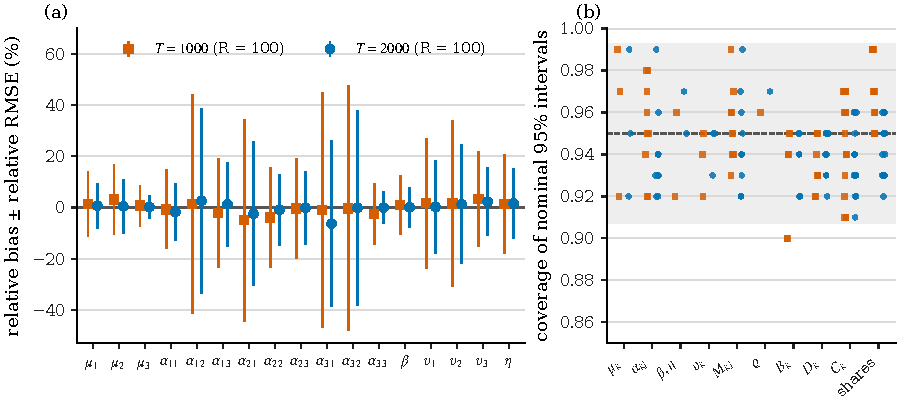
\includegraphics[width=6.0in]{figures/fig-sim-recovery.pdf}
\caption{E1, recovery by EM (synthetic data, $R=100$ per $T$). (a) Relative bias
(markers) $\pm$ relative RMSE (bars), in per cent, for the 17 parameters. (b) Coverage of
nominal $95\%$ intervals for the parameters and the derived quantities: multiplier entries
$M_{kj}$, spectral radius $\varrho$ and the surge components of E5. The grey band is the
$95\%$ Monte Carlo range around $0.95$ for $R=100$.}
\label{fig:sim-recovery}
\end{figure}

\begin{figure}[tbp]
\centering
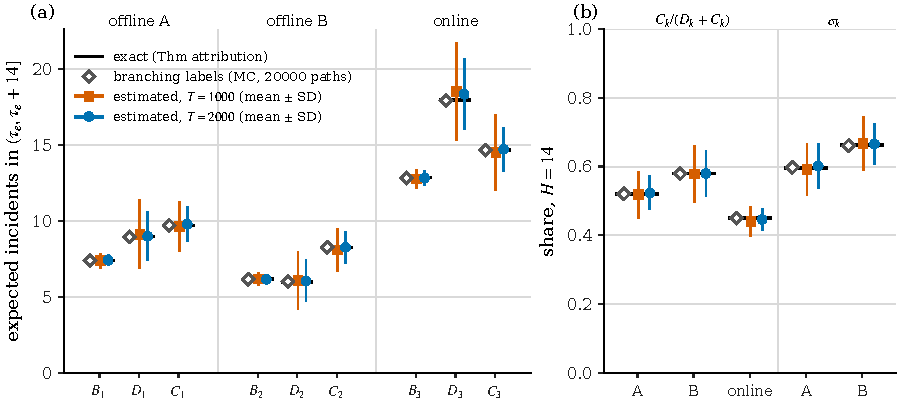
\includegraphics[width=6.0in]{figures/fig-sim-attribution.pdf}
\caption{E5, surge attribution after an event of size $S_e=3$ (synthetic data). (a) Expected
counts in $(\tau_e,\tau_e+14]$ by stream: exact values (\cref{thm:attribution}; lines),
branching-label Monte Carlo means (20{,}000 paths; diamonds), and estimates from the E1 fits
(mean $\pm$ SD over 100 replicates). (b) Contagion shares $C_k/(D_k+C_k)$ and online-channel
shares $\sigma_k$ at $H=14$, by stream.}
\label{fig:sim-attribution}
\end{figure}

\begin{figure}[tbp]
\centering
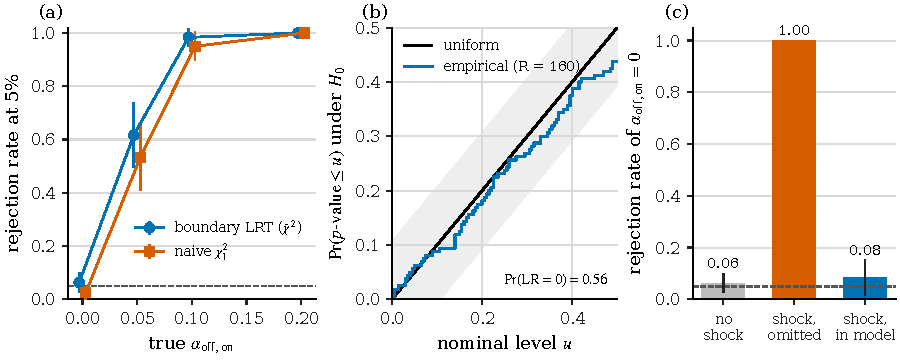
\includegraphics[width=6.0in]{figures/fig-sim-lrt.pdf}
\caption{E4, the test of $\alpha_{\mathrm{off},\mathrm{on}}=0$ (synthetic data; bars
$\pm1.96$ MC SE). (a) Rejection rate at the $5\%$ level against the true
$\alpha_{\mathrm{off},\mathrm{on}}$, for the chi-bar-square and the naive $\chi^2_1$
reference. (b) Empirical distribution function of the chi-bar-square $p$-values under
$H_0$ ($R=160$), with a $95\%$ Kolmogorov--Smirnov band; the $p$-value is $1$ whenever the
statistic is $0$. (c) Rejection rates without shocks, and with common shocks omitted from
or included in the model ($R=60$).}
\label{fig:sim-lrt}
\end{figure}

\FloatBarrier
\subsection{Monte Carlo standard errors}\label{app:sim-mcse}

Let $x_1,\dots,x_R$ be the estimates of a quantity with true value $x_0$ over $R$
replicates, with mean $\bar x$, standard deviation $s_x$ and errors $\varepsilon_r=x_r-x_0$.
\begin{itemize}
  \item \emph{Mean and bias.} The bias is $\bar x-x_0$. The MC SE of the mean and of the
  bias is $s_x/\sqrt R$. Medians are reported without MC SE.
  \item \emph{RMSE.} $\mathrm{RMSE}=(R^{-1}\sum_r\varepsilon_r^2)^{1/2}$, with MC SE
  $s_{\varepsilon^2}/(2\,\mathrm{RMSE}\sqrt R)$ by the delta method, where
  $s_{\varepsilon^2}$ is the standard deviation of the squared errors.
  \item \emph{Coverage and rejection rates.} For an estimated proportion $\hat\pi$, the
  MC SE is $\{\hat\pi(1-\hat\pi)/R\}^{1/2}$. The band of \cref{fig:sim-recovery}(b) is
  $0.95\pm1.96\,(0.95\times0.05/R)^{1/2}$.
  \item \emph{E5.} For each quantity, the mean over the $N=20{,}000$ paths has MC SE
  $(\hat\sigma^2/N)^{1/2}$, with $\hat\sigma^2$ the sample variance over paths, and
  $z=(\text{mean}-\text{exact})/\text{MC SE}$.
  \item \emph{E6.} Costs per window, Brier, CRPS and log scores and the mean forecast bias
  are averaged within each replicate; the MC SE is the standard deviation of the 12
  replicate averages divided by $\sqrt{12}$. Differences between two forecasters are
  paired: the MC SE is that of the 12 replicate differences. Alert rates, precision and
  recall are pooled over all 1800 windows and have no reported MC SE. The PIT statistic is
  $\chi^2=\sum_{b=1}^{10}(h_b-e)^2/e$, with $h_b$ the bin counts and $e$ the number of
  windows divided by 10, referred to $\chi^2_9$. The windows do not overlap and the outcomes
  are settled, so by \cref{lem:fc-pit}(b) the PIT values are independent under a correct
  forecast; the reference ignores the Monte Carlo error of the predictive distributions.
  The state ratios are ratios of means over all windows.
\end{itemize}
In the figures, error bars are $\pm1.96$ MC SE, except in \cref{fig:sim-recovery}(a)
($\pm$ relative RMSE), \cref{fig:sim-attribution} ($\pm1$ SD over replicates) and
\cref{fig:sim-thinning}(c) (no bars).

\subsection{Reproduction}\label{app:sim-repro}

From \texttt{papers/contagion/code/}, the commands
\begin{quote}\small
\texttt{OPENBLAS\_NUM\_THREADS=1 nice python run\_experiments.py -{}-workers 2}\\
\texttt{python make\_figures.py}
\end{quote}
run all six experiments, write \texttt{results/raw/E*.json} and
\texttt{results/sim\_results.json}, and then the figures and the tables
\texttt{tables/tab-sim-e1.tex}, \dots, \texttt{tab-sim-e6.tex}. With the current driver a
single run replaces the steps of \cref{app:sim-run}: E5 uses 20{,}000 paths, E2 includes
the long windows, E3 the three error levels and E6 the integrating forecasters, and the
seeds of every value stored earlier are unchanged. One experiment can be rerun with
\texttt{-{}-only E5} (E5 reads the stored E1 results when E1 is not run in the same
invocation); \texttt{-{}-augment-e2} repeats revision step (4); and
\texttt{-{}-merge-only} rebuilds the results file from the raw files. The option
\texttt{-{}-quick} runs tiny configurations in seconds; the tests in
\texttt{code/tests/test\_experiments.py} use it to check the output schema, the absence of
failed replicates, that two runs give identical results and that the integrating
forecasters leave the other E6 forecasters unchanged. With the recorded software versions,
the seeds determine every replicate. We have not checked whether other versions of NumPy or
SciPy reproduce the results to the last digit.
}{}
% Candidate data sources, the full pre-registered plan and the full ethics protocol.
\IfFileExists{appendix/P-plan-ethics.tex}{% =====================================================================
%  Appendix (TEXT-REVISER, revision 1): candidate data sources, the full
%  pre-registered analysis plan and the full ethics protocol, moved out of
%  Sections 2, 9 and 10 to shorten the main text. Every label is preserved.
% =====================================================================
\section{Candidate data sources}\label{app:data}

This appendix gives the source-by-source detail summarised in \cref{sec:data-incidents}.
For every source we record what can be checked in the provider's own documentation: the
timestamp the record carries, its temporal and geographic resolution, the anti-Jewish bias
category, and how the data can be obtained. Properties that we could not confirm from
primary documentation at the time of writing (November 2026) are marked as such and are not
used in any argument. \Cref{tab:data-streams} summarises the candidate streams.

\subsection{Incident streams}\label{app:data-incidents}

\paragraph{City-level open data: NYPD hate crimes.}
The New York City Police Department publishes a file of confirmed hate-crime
incidents on the NYC Open Data portal (dataset \texttt{bqiq-cu78})
\citep{nypdhate}, beginning in 2019. According to the portal's data
dictionary, \emph{Complaint Year Number} and \emph{Month Number} give the
year and month in which the incident occurred, and \emph{Record Create Date}
gives the date on which the report was filed. A \emph{Bias Motive
Description} field holds the NYPD's bias category, whose values include
\texttt{ANTI-JEWISH}. Geography is given by the complaint precinct, the
patrol borough and the county; each of the city's five counties is
coterminous with a borough. For point-process work the file thus has a
two-level time structure: the occurrence time is interval-censored to a
calendar month, while the report date is known to the day. We treat the
record-creation date as a report date and model the delay between occurrence
and record creation explicitly (\cref{sec:data-delays}), with the
occurrence month as a constraint. Whether day-level occurrence dates can be
obtained from the NYPD, for example under a data-use agreement, is an open
feasibility question for the pilot (\cref{sec:plan}); we do not assume it.
Changes to reporting systems are structural breaks for time-series use. The
New York State Comptroller reported that the state's Division of Criminal
Justice Services did not publish 2023 hate-crime data for New York City
because of the NYPD's transition in data-reporting systems as part of its
move to NIBRS \citep{osc2024hate}. \Citet{rosenbaum2025} analyses NYPD
administrative hate-crime records for 2019--2024 at monthly resolution.
Adjusting for the Jewish population of each borough, the study reports
that monthly anti-Jewish hate crimes were on average about twice as common
in the first year of the Israel--Hamas war as in the preceding years of the
study period (prevalence ratio 1.97, 95\% CI 1.64--2.35). Monthly
resolution suffices for such before--after contrasts but not for kernels
on the scale of days.

\paragraph{FBI NIBRS.}
The FBI's Uniform Crime Reporting Program retired its Summary Reporting
System on 1 January 2021 and moved to collection through the National
Incident-Based Reporting System (NIBRS) \citep{fbi2026nibrs}. For hate
crimes, however, the FBI reopened the 2021 collection to summary-format
submissions \citep{fbi2023supp}. According to the Congressional Research
Service, it has accepted both formats since 2022 \citep{crs2025hate}. Each
NIBRS incident carries the mandatory Data Element~3, \emph{Incident
Date/Hour}. The date is recorded as \texttt{YYYYMMDD} and the hour on a
24-hour clock. When the incident date is unknown, the report date is entered
instead and flagged with a report-date indicator
\citep{fbi2025nibrs,fbi2025nibrstech}. Anti-Jewish bias is code~21 of Data
Element~8A, \emph{Bias Motivation} \citep{fbi2025nibrs}. The geographic unit
is the reporting agency, identified by its ORI number. NIBRS submissions
thus supply occurrence dates, and hours where recorded, for individual
anti-Jewish incidents. For summary-format submissions we have not confirmed
comparable date fields, so the stream is restricted to NIBRS records. The
data are also slow. National statistics for data year 2024 were released on
5 August 2025 \citep{fbi2025release}, so for that year the lag from
occurrence to national availability was roughly 7 to 19 months, depending
on when in the year an incident occurred. Agency participation varies by
agency and year; the companion paper models it.

\paragraph{ADL Audit and H.E.A.T.\ Map.}
ADL describes its annual Audit as covering criminal and non-criminal
incidents of harassment, vandalism and assault, as reported to ADL by
victims, law enforcement, the media and partner organisations
\citep{adl2025audit}. An ADL stream therefore measures a different quantity
from a police stream, and the two reach the record through different funnels
(\cref{sec:data-thinning}). ADL states that since 7 October 2023 the Audit
has included certain expressions of opposition to Zionism and of support for
violent resistance against Israel or Zionists, while continuing to exclude
legitimate political protest \citep{adl2025audit}. For a point-process model
this matters for a structural reason, separate from any substantive
judgement. A change in recording scope at a date that is also a candidate
shock time $\tau_e$ is not identified separately from the shock term unless
the change is modelled explicitly. An ADL stream therefore needs a scope-break
indicator in $\mu_k(t)$, or records coded under a constant scope rule. ADL's
H.E.A.T.\ Map (Hate, Extremism, Antisemitism, Terrorism) publishes
incident-level listings that can be downloaded as a CSV file, with some
details removed to protect victims' privacy \citep{adlheatmap}. We have not
confirmed whether the listed date is the date of occurrence or of report to
ADL, nor how redaction affects dates. These checks are part of the pilot's
feasibility stage.

\paragraph{CST (United Kingdom).}
The Community Security Trust records antisemitic incidents in the United
Kingdom and publishes annual reports, most recently for 2025
\citep{cst2026incidents}. CST data would serve as an international comparison
stream. That report illustrates a further threat to time-series analysis.
CST states that since March 2024 a technical problem has disrupted the flow
of reports to it from the Metropolitan Police \citep{cst2026incidents}. In
the notation of \cref{sec:data-thinning}, an interruption in a referral feed
is a step change in the recording probability $p_k(t)$, which a model with
constant $p_k$ would read as a change in the incident process itself.
Incident-level records with dates would require a data-sharing agreement,
and a CST stream is therefore conditional.

\begin{table}[!htbp]
\centering
\caption{Candidate data streams for the pre-registered analysis. ``TBC'':
not confirmed from the provider's documentation at the time of writing; to
be confirmed before registration. Delays are from occurrence to
availability to analysts.}
\label{tab:data-streams}
\footnotesize
\setlength{\tabcolsep}{3pt}
\renewcommand{\arraystretch}{1.15}
\begin{tabularx}{\textwidth}{@{}>{\raggedright\arraybackslash}p{2.35cm}
  >{\raggedright\arraybackslash}X
  >{\raggedright\arraybackslash}p{2.2cm}
  >{\raggedright\arraybackslash}X
  >{\raggedright\arraybackslash}p{2.6cm}@{}}
\toprule
Stream & Time stamp (resolution) & Geography & Delay to availability & Access \\
\midrule
NYPD hate crimes \citep{nypdhate}
  & Occurrence: month; record creation: day. From 2019.
  & Precinct, patrol borough, county
  & Report delay bounded by occurrence month and record date; refresh schedule TBC
  & Public download (NYC Open Data) \\
FBI NIBRS \citep{fbi2025nibrs,fbi2026nibrs,crs2025hate}
  & Incident date and hour; report date substituted (flagged) if incident date unknown. NIBRS from 2021; hate-crime collection also accepts summary format since 2022.
  & Reporting agency (ORI)
  & Annual national release; data year 2024 released 5 Aug.\ 2025
  & Public (FBI Crime Data Explorer) \\
ADL Audit / H.E.A.T.\ Map \citep{adl2025audit,adlheatmap}
  & Incident date listed; occurrence vs.\ report date TBC. Scope change from 7 Oct.\ 2023.
  & Place listed; resolution TBC
  & TBC
  & Public map; CSV download with redactions \\
CST (UK) \citep{cst2026incidents}
  & TBC
  & TBC
  & Annual report; 2025 report published Feb.\ 2026
  & Incident-level records by agreement (TBC) \\
ACLED \citep{raleigh2010}
  & TBC
  & Event location
  & TBC
  & Provider terms (TBC) \\
GDELT \citep{leetaru2013}
  & TBC
  & Event location
  & TBC
  & Provider terms (TBC) \\
Platform data \citep{eu2022dsa}
  & Post time stamps (binned for analysis)
  & Varies
  & Depends on access route
  & DSA Art.~40 procedure; status TBC \\
Classifier volume \citep{kornsteinlab2026detection,kornsteinlab2026measurement}
  & Bin chosen by design (e.g.\ day)
  & None or coarse
  & Construction lag only
  & Lab-constructed from a defined corpus \\
\bottomrule
\end{tabularx}
\end{table}

\FloatBarrier
\subsection{Platform data access}\label{app:data-platform}

Article~40 of the EU Digital Services Act provides a procedure by which
vetted researchers may obtain data from very large online platforms and
very large online search engines for research that contributes to the detection,
identification and understanding of systemic risks in the Union. It also
contains a separate provision on access to publicly accessible data, and it
leaves technical conditions to delegated acts \citep{eu2022dsa}. Whether a
given project qualifies, and on what terms, is decided through that
procedure. We have not confirmed its operational status for the platforms
and periods of interest, and the plan in \cref{sec:plan} treats online
streams as optional, so that the offline analysis does not depend on them.
The terms of any research interface used will be recorded at registration.

\subsection{Prior empirical literature}\label{sec:data-lit}

\Citet{mohler2011} developed self-exciting point-process models of
crime; \citet{reinhart2018} reviews spatio-temporal versions and their
applications. Related applications include a spatiotemporal test of whether
gun violence is contagious \citep{loeffler2018} and self-exciting models of
civilian deaths in Iraq \citep{lewis2012}. For hate crime specifically,
\citet{king2013} study the temporal clustering of hate-motivated offending.
Two studies examine links between online content and offline hate crime:
\citet{muller2021} study social media and hate crime, and
\citet{williams2020} examine anti-Black and anti-Muslim social-media posts
as predictors of offline racially and religiously aggravated crime. For
anti-Jewish incidents, \citet{rosenbaum2025} compares monthly NYPD counts
before and after a salient external event (see above). We use this
literature to motivate the questions, not as prior estimates. None of these
studies estimates a multivariate branching matrix for antisemitic incidents,
and our framework does not take its parameter values from them. Separating
exogenous shocks from contagion is the identification problem of
\cref{sec:identification}.

\section{The pre-registered analysis plan in full}\label{app:plan}

This appendix sets out in full the analysis plan summarised in \cref{sec:plan}, which we
intend to register before any outcome data are examined. It fixes the candidate data, the
estimands, the procedure for listing external events, the model hierarchy and its tests,
the sensitivity analyses, the validation checks and the decision rules. The numerical
settings below (horizons, thresholds, grids, replicate numbers) are proposals. They will be
frozen at registration; any change made before registration will be documented, and any
change made after it will be reported as a deviation. The simulation study
(\cref{sec:simulation}) evaluates, on synthetic data with known ground truth, some of the
tools these rules rely on: EM estimation, surge attribution, the boundary test, the
thinning correction and a plug-in alert. It does not evaluate the block tests of
\cref{sec:plan-models}, the placebo calibration, the time-rescaling check, the Bayesian fit
or the selection and decision rules themselves; they are checked in the synthetic dry run
(V4). No part of the plan has yet been carried out on real data.

\subsection{Candidate pilot}\label{sec:plan-pilot}

\paragraph{Setting.}
The candidate pilot is New York City, using the NYPD hate-crime file
described in \cref{sec:data-incidents} \citep{nypdhate}. We restrict it
to records whose bias motive is \texttt{ANTI-JEWISH} and use the period from
2019 onwards. The offline streams $k$ are the five boroughs. Sparse streams
are handled by shrinkage on $\Amat$ (\cref{sec:estimation}), not by merging
streams on the basis of observed counts, which would let outcome data shape
the model. The offence category serves as a mark in a secondary analysis.
The final 12 months of data available at the freeze date form the hold-out
test period, and all earlier data form the training period.

\paragraph{Two designs, chosen before outcome data are seen.}
The NYPD file records the month of occurrence and the day of record creation
(\cref{sec:data-incidents}). The design is chosen on data availability
alone:
\begin{enumerate}[(A)]
  \item \emph{Design A} (conditional): if day-level occurrence dates can be
  obtained under a data-use agreement, the model is fitted to occurrence
  days, with within-day ties handled as in \cref{sec:data-needs}.
  \item \emph{Design B} (default): the model is fitted to record-creation
  dates, treated as a report-time process. The occurrence month enters as an
  interval constraint on each delay, and the delay distribution is modelled
  explicitly (\cref{sec:data-delays}). Contagion parameters then describe the
  report-time process, and sensitivity to the delay model is analysis~S4.
\end{enumerate}

\paragraph{Additional streams.}
Three further sources are conditional on access being confirmed during the
feasibility stage: (i) a classifier-based online volume series
(\cref{sec:data-online}); (ii) an ADL stream, if its export provides
day-level dates; and (iii) a CST stream as an international replication. A
national NIBRS analysis of anti-Jewish incidents is retrospective only,
because of the release lag (\cref{sec:data-incidents}). If a conditional
stream is unavailable it is dropped, and the primary analysis is unaffected.

\paragraph{Feasibility gates.}
Before registration we will: confirm the data dictionaries and archive the
data vintages (F1); choose between Designs A and B (F2); record the
licence terms of the event sources (F3); confirm or abandon the online
streams (F4); and obtain ethics approval (F5; \cref{sec:ethics}).

\subsection{Primary estimands}\label{sec:plan-estimands}

\begin{enumerate}[E1.]
  \item \emph{Branching matrix.} The matrix $\Amat=[\alpha_{kj}]$ for the
  recorded streams has three parts: the diagonal $\alpha_{kk}$
  (within-borough self-excitation); the off-diagonal offline entries
  (cross-borough excitation); and, when online streams are included, the
  online$\to$offline and offline$\to$online blocks. We report each entry
  with its interval, together with $\spr(\Amat)$ and
  $\Mmat=(\Imat-\Amat)^{-1}$. Estimates are reported on the recorded scale
  first. Thinning-corrected values (\cref{thm:thinning}) are reported
  alongside and labelled as model-based (\cref{sec:data-thinning}).
  \item \emph{Surge decomposition.} For each pre-registered event $e$ and
  stream $k$ we report the decomposition $\E[N_k(\tau_e,\tau_e+H]] =
  B_k + D_k + C_k$ of \cref{thm:attribution} and, where online streams are
  included, the online$\to$offline spillover share. The primary horizon is
  $H=14$ days, with $H\in\{7,28\}$ as secondary horizons. Results are
  summarised by event class. Event-level results appear in an appendix under
  neutral identifiers (\cref{sec:plan-events}).
  \item \emph{Alert performance.} We evaluate the rule of \cref{thm:alert}
  and \cref{alg:alert}, with window $\Delta_{\mathrm a}=7$ days. For each stream the
  surge threshold $c$ is the 95th percentile of the training-period
  distribution of 7-day counts. The cost ratio $c_{\mathrm{miss}}/c_{\mathrm{FA}}$
  is agreed with community-security partners before registration, with
  $\{2,5,10\}$ as the default grid. Metrics are the hit rate, false-alarm
  rate, realised cost and the Brier and log scores for the exceedance event.
  Two baselines serve as comparators: the background-only model M0 and a
  persistence rule that raises an alert when the previous window exceeded
  $c$.
\end{enumerate}
Secondary estimands are the kernel time scales, the class-level shock
loadings $\upsilon_k$ and the seasonal components of $\mu_k(t)$.

\subsection{Pre-specified external events}\label{sec:plan-events}

The event list is fixed by the following procedure. Every step is completed
before the analysis team loads any incident data for the study period.
\begin{enumerate}[1.]
  \item \emph{Classes.} Event classes are defined by type: (a) onset or
  major escalation of armed conflict; (b) terrorist or other mass-casualty
  attacks; (c) high-profile public statements by public officials or other
  prominent figures. The operational definitions are applied identically
  whatever the location, the parties, the perpetrators or the victims. We do
  not select events by their presumed relevance to antisemitism. Relevance
  is estimated through the loadings $\upsilon_k$, and events that are
  irrelevant to the outcome should receive loadings near zero. A secondary
  list restricts the pool to events whose coverage matches a keyword list
  that is fixed and deposited in advance.
  \item \emph{Salience threshold.} For each candidate event, a salience
  index is computed from the event datasets alone
  (\cref{sec:data-events}). It is the coverage attributed to the event over
  $[\tau_e,\tau_e+2\text{ days}]$, divided by the median daily coverage over
  the preceding 365 days. An event enters the list if its index exceeds a
  threshold $s^\star$. The threshold is set, using event data only, so that
  the list contains between 10 and 30 events over the study period. The
  size $S_e$ is the logarithm of the index.
  \item \emph{Blind coding.} Two coders independently review the candidates
  above the threshold. They merge duplicates, assign each event to a class
  and set $\tau_e$ to the time of first public report in the pilot city's
  time zone, to the day (or the hour under Design A). The coders have no
  access to incident data, which a separate data custodian holds until the
  freeze. Agreement is reported as Cohen's $\kappa$ for class and as the
  share of $\tau_e$ that agree to within one day. A third coder resolves
  disagreements. Events less than 48 hours apart are merged into a single
  shock at the earlier time.
  \item \emph{Freeze.} The list ($\tau_e$, class, $S_e$, source identifiers)
  is written to a file. The file's SHA-256 hash is posted with the
  registration and the file is deposited with the registry. Events after the
  freeze, which are needed for prospective evaluation, are coded under the
  same rules within seven days and appended with time-stamped hashes.
  \item \emph{Neutral identifiers.} Each event is reported by class and
  date. Descriptions follow the conventions of \cref{sec:ethics}.
\end{enumerate}

\subsection{Model hierarchy, block tests and selection rules}\label{sec:plan-models}

The models are nested:
\begin{enumerate}
  \item[M0] Background only: $\mu_k(t)=\exp(B(t)^\top\theta_k)$. The basis
  $B$ is a cubic B-spline in calendar time with knot spacing $h_b=60$ days, so that the
  number $K_b$ of basis functions grows with the length of the study period, plus
  day-of-week effects and indicators for a holiday calendar fixed in advance.
  \item[M1] M0 plus shocks $\sum_e\upsilon_k S_e\psi_k(t-\tau_e)$, with an
  exponential response kernel $\psi_k$; the loading $\upsilon_k$ and the
  kernel are specific to each stream and shared by all events of a class.
  \item[M2] M1 plus self-excitation (diagonal $\Amat$).
  \item[M3] M2 plus cross-stream offline excitation (the off-diagonal entries of the
  offline block of $\Amat$).
  \item[M4] M3 plus the online$\to$offline and offline$\to$online blocks, when online
  streams are available.
\end{enumerate}
The kernels are exponential, with one common decay rate within each block: the diagonal
(M2), the offline off-diagonal entries (M3), and each of the two online blocks (M4). We
estimate by maximum likelihood via EM (\cref{alg:em}), with parametric bootstrap intervals
from 500 replicates. A Bayesian fit with shrinkage on $\Amat$ (\cref{sec:est-bayes}) is
co-primary for M3 and M4.

\paragraph{Block tests.} Each step of the hierarchy adds a block of parameters that share
one rate: the loadings with their response rate (M0$\to$M1), or a block of entries of
$\Amat$ with its common decay (M1$\to$M2, M2$\to$M3, and for M4 first the online$\to$offline
block, then the offline$\to$online block). Under the null that every entry of the block is
zero, that rate is not identified, so the chi-bar-square reference
\eqref{eq:est-chibar} does not apply (\cref{rem:est-lrt}(i)). Each step is therefore decided
by the following registered test.
\begin{enumerate}[(i)]
  \item \emph{Statistic.} The sup-LR statistic \eqref{eq:est-suplr},
  $\mathrm{LR}_{\sup}=\max_g2\{\ell_T(\hat\vartheta_{j+1}(\beta_g))-\ell_T(\tilde\vartheta_j)\}$,
  where $\tilde\vartheta_j$ is the fit of the smaller model and
  $\hat\vartheta_{j+1}(\beta)$ the fit of the larger model with the new block's rate fixed
  at $\beta$ and every other parameter free.
  \item \emph{Grid.} $G=9$ rates whose half-lives $\log2/\beta_g$ are equally spaced on the
  log scale from $0.5$ to $21$ days ($0.5,\,0.8,\,1.3,\,2.0,\,3.2,\,5.2,\,8.3,\,13.2,\,21$
  days). The longest half-life is about a third of the knot spacing $h_b$, which keeps the
  cascade time scale apart from the background (\cref{sec:est-mle}).
  \item \emph{Reference.} The parametric bootstrap \eqref{eq:est-pboot} from the fit of the
  smaller model, with the observed calendar and $B=499$ replicates. In each replicate both
  models are refitted, the larger one at every grid value, starting from the null fit with
  small positive block entries (\cref{app:comp-tests}). The step is taken if
  $p_{\mathrm B}\le0.05$. The upcrossing approximation $p_{\mathrm D}$
  (\cref{app:est-davies}) is reported as a secondary quantity only.
  \item \emph{Order.} The block tests are applied in the fixed order of the hierarchy, each
  at level $0.05$ and only if the previous step was taken. This fixed-sequence procedure
  controls the family-wise error rate of the block decisions at $0.05$.
  \item \emph{Entries and the Holm family.} Within the blocks that were accepted, each entry
  $\alpha_{kj}$ is tested by the boundary test \eqref{eq:est-chibar}, whose decay is
  identified through the other entries of its block. If every other entry of the block is
  estimated as zero under the entry's null, that entry is tested with the sup-LR procedure
  of (i)--(iii) instead. All entry-level tests in the accepted blocks form one family, and
  Holm's procedure \citep{holm1979} controls its family-wise error rate at $0.05$. Decision
  rules D1 and D2 refer to these Holm-adjusted tests.
  \item \emph{Fallbacks.} The synthetic dry run (V4, \cref{sec:plan-validation}) checks the
  size and the cost of the block tests before any real data are loaded. If only the cost
  check fails, the score-based sup-statistic of \cref{app:est-davies} replaces the sup-LR
  statistic, with the same grid and $B=999$ replicates. If the size check fails, the block's
  rate is fixed in advance at the median of the grid (half-life $3.2$ days), and the block
  is tested by the likelihood-ratio statistic at that rate, with the parametric bootstrap
  reference of (iii). If that test also fails the size check, the step is decided by the
  out-of-sample log score alone, its excitation estimates are reported as exploratory, and
  no contagion claim under D1 or D2 is made for that block. The fallback used is reported
  for every step.
\end{enumerate}

\paragraph{Selection rules.} Moving from $\mathrm{M}j$ to $\mathrm{M}(j{+}1)$ requires both
of the following:
\begin{enumerate}[(a)]
  \item the block test of the step rejects at level $0.05$;
  \item the out-of-sample log score improves.
\end{enumerate}
The reported model is the largest model that meets both criteria. Estimates from every
model in the hierarchy are reported as well.

\subsection{Sensitivity analyses}\label{sec:plan-sens}

\begin{enumerate}[S1.]
  \item \emph{Background flexibility.} We vary the knot spacing
  $h_b\in\{30,60,120,365\}$ days and also fit a random-walk log-background.
  A misspecified, too rigid background produces spurious contagion
  (\cref{thm:spurious}), and second-order structure cannot settle the
  question (\cref{thm:equiv}). Self-excitation that vanishes under a more
  flexible background while goodness of fit remains acceptable is reported
  as not robustly distinguishable from background variation. An overly
  flexible background can absorb genuine contagion. In the simulation study a
  spline background removed the spurious contagion of slow regime switches but
  not that of fast unrecorded shocks (\cref{sec:sim-spurious}); how much
  genuine contagion it absorbs was not studied and is checked in the
  synthetic dry run (V4).
  \item \emph{Thinning.} We use (a) posterior draws of $p_k$ from the
  companion paper, mapped to streams as in \cref{sec:data-thinning}; (b) a
  grid $p_k\in\{0.1,0.25,0.5,0.75,1\}$; and (c) salience-dependent recording,
  $p_k(t)=p_k\{1+\varepsilon\sum_e\psi(t-\tau_e)\}$ with
  $\varepsilon\in\{0,0.25,0.5,1\}$ (capped at one), which violates the
  independence condition of \cref{thm:thinning}. In addition, (d) known
  recording breaks, such as reporting-system transitions, scope changes and
  interrupted referral feeds (\cref{sec:data-incidents}), enter $\mu_k(t)$
  as step indicators, and results are reported with and without the
  affected periods.
  \item \emph{Kernel family.} We compare exponential, gamma, power-law and
  nonparametric (histogram) kernels \citep{marsan2008}.
  \item \emph{Delay distribution.} Under Design B we fit the delay
  distribution in three versions: estimated from the month and
  record-creation bounds; with its scale shifted by $\pm50\%$; and with a
  heavy-tailed (log-normal) form. We compare the report-time analysis with
  an occurrence-month aggregate analysis. Nowcast corrections follow
  \cref{prop:nowcast}.
  \item \emph{Event list.} We halve and double $s^\star$, drop each event in
  turn, compare class-specific and pooled loadings, and vary the shock
  kernel $\psi$.
  \item \emph{Spatial resolution.} We compare boroughs with patrol boroughs.
  \item \emph{Online measurement error.} We compare uncorrected and corrected
  series (\cref{eq:data-classerr}), with period-specific error rates and
  propagated uncertainty.
  \item \emph{Ties.} We compare at least 20 within-day randomisations with
  the discrete-time INAR fit (\cref{eq:inar}).
\end{enumerate}

\subsection{Validation}\label{sec:plan-validation}

\begin{enumerate}[V1.]
  \item \emph{Goodness of fit.} Following \citet{brown2002}, we apply the
  time-rescaling theorem (\cref{prop:rescaling}) stream by stream: a
  Kolmogorov--Smirnov test on rescaled inter-event times, with times
  randomised within the recorded resolution. Because the parameters are
  estimated, the reference distribution is obtained by parametric
  bootstrap.
  \item \emph{Out-of-sample performance.} We compute log scores for daily
  counts \citep{gneiting2007} and randomised PIT histograms for calibration
  \citep{dawid1984,gneiting2007b}, using rolling-origin one-step and
  $\Delta_{\mathrm a}$-step forecasts over the test period.
  \item \emph{Placebo shocks.} Placebo calibration is done for one event class at a time
  (\cref{sec:est-placebo}). For each class we draw 1{,}000 placebo calendars with the same
  number of events as the real class, and permute the real sizes over them. Their dates are
  drawn uniformly from \emph{all} days of the training period, holidays included, subject
  only to the 48-hour merging rule of \cref{sec:plan-events} within each calendar, and
  without reference to the real dates of that class. Excluding holidays, or any other set of
  days on which a real event could fall, would break the exchangeability on which the rank
  test rests. The base model is the selected model with that class removed. The real class
  and each placebo calendar are added to the base model in turn, as a shock class, and the
  same statistics are computed for all of them. The rejection frequency of the placebo
  loading tests at nominal level $0.05$ is the empirical false-positive rate of the shock
  test. The rank of each real-event direct component $D_k$ among its placebo counterparts is
  reported. The rank $p$-value is exact under the randomisation hypothesis of
  \cref{lem:est-placebo}, that the real dates are exchangeable with draws from this design;
  otherwise it is reported as a calibration, not as a test. If the empirical
  false-positive rate exceeds $0.10$, inference on shocks uses the placebo distribution in
  place of the asymptotic reference.
  \item \emph{Synthetic dry run.} Before any real data are loaded, the full pipeline is run
  on synthetic data generated as in \cref{sec:simulation}, at the pilot's number of
  streams, length of study period and calendar size. It uses $R=200$ datasets from each of
  two configurations: a null configuration without excitation (M1), and an alternative
  with self-excitation $0.3$ and cross-stream entries $0.05$, both with a spline
  background. It checks (a) the size of each block test of \cref{sec:plan-models} at a
  configuration that satisfies its null (the null configuration for the excitation blocks,
  and the same configuration without shocks for M0$\to$M1), which passes if the rejection
  rate is at most $0.075$ (Monte Carlo standard error about $0.015$); (b) its cost, which passes if one block test takes at
  most seven days on the project's computing allocation; (c) the coverage of the intervals
  for $\alpha_{kj}$ and for the surge decomposition at the alternative; and (d) the
  selection and decision rules, including whether a spline background with spacing $h_b$
  absorbs genuine contagion. Failures of (a) or (b) trigger the fallbacks of
  \cref{sec:plan-models}.
\end{enumerate}

\subsection{Decision rules}\label{sec:plan-decisions}

\begin{enumerate}[D1.]
  \item \emph{Self-excitation} in stream $k$ is claimed only if: the test of
  $\alpha_{kk}=0$ rejects after the Holm correction; the 95\% interval for
  $\alpha_{kk}$ excludes zero under the most flexible background in S1;
  goodness of fit (V1) is not rejected at level $0.01$; and the placebo
  false-positive rate (V3) is at most $0.10$. Otherwise we report that
  self-excitation is not distinguishable from background variation at the
  available resolution.
  \item \emph{Cross-stream and online$\to$offline excitation} are claimed
  under the same criteria applied to $\alpha_{kj}$. They are described as
  Granger-type predictive dependence (\cref{prop:granger}) and never as
  causation.
  \item \emph{Surge decompositions} are reported for every pre-registered
  event, whatever its size or significance. A surge is described as
  predominantly due to contagion only if the 95\% interval for
  $C_k/(D_k+C_k)$ lies above $0.5$ under the primary model and under the
  S1 and S2 variants.
  \item \emph{Thinning-corrected} branching ratios are never reported
  without the $p_k$ used and the S2 range.
  \item \emph{Alerts} are recommended for operational use with partners only
  if, in the test period, the rule's realised cost is lower than that of
  both baselines, with a bootstrap 95\% interval for the difference that
  excludes zero, and the PIT shows no marked miscalibration. Otherwise the
  alert analysis is reported as a research result only.
  \item \emph{Null results and deviations} are reported in full.
\end{enumerate}

\subsection{Replication package}\label{sec:plan-replication}

The package will contain:
\begin{enumerate}[(i)]
  \item the estimation and simulation code with a pinned environment;
  \item the frozen event list and its hash;
  \item acquisition scripts with dataset identifiers, vintages, download
  dates and SHA-256 checksums;
  \item derived counts by stream, at the resolutions and subject to the
  small-cell rules of \cref{sec:ethics-irb};
  \item for restricted streams (platform or partner data), the code together
  with a synthetic dataset of the same structure;
  \item all results as machine-readable files, with scripts that regenerate
  every table and figure; and
  \item the deviations log.
\end{enumerate}
Raw records are redistributed only where the provider's terms permit.

\subsection{Timeline}\label{sec:plan-timeline}

\Cref{tab:plan-timeline} gives the timeline in months from the start of the
feasibility stage.

\begin{table}[!htbp]
\centering
\caption{Timeline of the pre-registered analysis, in months from the start
of the feasibility stage. Each gate must be passed before the next phase
begins.}
\label{tab:plan-timeline}
\footnotesize
\renewcommand{\arraystretch}{1.15}
\begin{tabularx}{\textwidth}{@{}l l >{\raggedright\arraybackslash}X >{\raggedright\arraybackslash}p{4.2cm}@{}}
\toprule
Phase & Months & Activities & Gate / output \\
\midrule
P0 Feasibility & 0--2 & Confirm data dictionaries and access terms (F1--F4); choose Design A or B; submit for ethics review & Ethics approval; design fixed \\
P1 Events and registration & 2--3 & Blind coding; freeze event list; register plan & Time-stamped registration; hash deposited \\
P2 Dry run & 3 & Full pipeline on synthetic data (V4) & Coverage and selection rules checked \\
P3 Training fit & 4--6 & Fit M0--M4; apply selection rules & Selected model \\
P4 Test evaluation & 7 & V1--V3; back-test of alerts & Out-of-sample report \\
P5 Sensitivity & 7--9 & S1--S8 & Robustness tables \\
P6 Reporting & 9--11 & Paper; replication package; partner debrief under \cref{sec:ethics} & Public release \\
P7 Prospective & 12--24 & Prospective alert evaluation under embargo & Embargoed evaluation report \\
\bottomrule
\end{tabularx}
\end{table}

\FloatBarrier
\section{The ethics protocol in full}\label{app:ethics}

This appendix gives in full the protocol summarised in \cref{sec:ethics}. It accompanies
the plan of \cref{app:plan} and complements the companion paper's protocol for victim
privacy and record linkage \citep{kornsteinlab2026darkfigure}.

\subsection{Risks of forecasting}\label{sec:ethics-risks}

\paragraph{Stigmatisation.}
A map of elevated predicted intensity can be read as a statement about the
people who live in an area. That reading applies to neighbourhoods where
Jewish residents are targeted, which can come to be seen as ``dangerous''.
It applies equally to any community that observers might wrongly treat as a
source of incidents. The model contains no information about perpetrators,
and its spatial units are recording areas, not communities. Alerts and published maps are therefore
at the borough level or coarser, and never street- or venue-level heat maps.
Finer units used in sensitivity analysis S6 are reported only as summary
statistics. No output ranks neighbourhoods or communities.

\paragraph{Self-fulfilling and self-defeating alerts.}
An alert can change what it predicts. Publicity can raise reporting, which
inflates recorded counts (the time-varying $p_k$ of analysis S2). Protective
deployment can prevent incidents, which makes a correct alert look like a
false alarm. Either effect contaminates prospective evaluation. Alerts
during the prospective period (phase P7) are therefore shared only under the
protocol below, and evaluation reports state which alerts were acted on.

\paragraph{Information hazards.}
Forecasts that name ``hot'' dates or locations could help someone planning
an attack, and could encourage imitation. We therefore publish methods,
code and retrospective results, but no live or near-live forecasts and no
forecast tied to a specific site. Retrospective results are released only
after an embargo (\cref{sec:ethics-disclosure}).

\subsection{Responsible disclosure of alerts}\label{sec:ethics-disclosure}

Alerts produced during the prospective evaluation are handled as follows.
\begin{enumerate}[1.]
  \item \emph{Recipients.} Alerts go only to vetted community-security
  partners, and to a police liaison where the partner agreement provides for
  this. Each partner signs an agreement that limits use to protective
  purposes, such as security staffing and victim support, and excludes
  enforcement targeting of any community.
  \item \emph{Content.} An alert gives the borough or coarser area, the
  window $\Delta_{\mathrm a}$, the predicted probability of exceeding the threshold
  with its uncertainty, and a fixed statement of the model's limitations.
  It contains no individual-level information and no attribution to
  persons, groups or communities.
  \item \emph{Human review.} A named member of the research team reviews
  every alert before release, and may withhold an alert that is plainly
  driven by a data artefact.
  \item \emph{Channel and logging.} Alerts are sent over an encrypted
  channel. Each alert, the decision to release or withhold it, and the
  partner's acknowledgement are logged for audit.
  \item \emph{Embargo.} Alerts are not published. Aggregate evaluation
  results (hit and false-alarm rates by quarter and borough) are published
  no earlier than 90 days after the end of the period they cover.
  \item \emph{Suspension.} Alerts are suspended if rolling calibration
  deteriorates beyond a pre-specified tolerance, or if a partner reports
  misuse.
\end{enumerate}

\subsection{Language and attribution}\label{sec:ethics-language}

The model attributes \emph{timing}, not blame. A positive shock loading
$\upsilon_k$, or a large direct component $D_k$ after event $e$, means that
recorded incidents in stream $k$ rose after $\tau_e$ by more than the
background and the contagion terms predict. It does not mean that the
parties to the event, the communities associated with them, or the people
who discussed it caused any incident. Incidents are committed by
individual perpetrators, about whom the model contains no information. We
therefore:
\begin{enumerate}[(i)]
  \item describe events as \emph{salient external events} of a stated class
  and date, and do not characterise them politically;
  \item never describe a community, nationality or religious group as a
  source, driver or cause of incidents;
  \item phrase every result in terms of recorded incidents and statistical
  association; this includes the online$\to$offline coefficients, which
  are Granger-type (\cref{prop:granger}); and
  \item report event-level decompositions in an appendix under neutral
  identifiers, with class-level summaries in the main text.
\end{enumerate}

\subsection{Political neutrality}\label{sec:ethics-neutrality}

The paper takes no position on any political conflict, government, movement
or public figure. Neutrality is built into the procedure, not just asserted:
event classes are defined by type and apply to all parties alike
(\cref{sec:plan-events}); the event list is frozen before outcome data are
seen, so events cannot be selected after the fact; every pre-registered
event is reported whatever the result (rule D3); and the event-coding rules
and frozen list are public. Before registration, the event-coding protocol
will be reviewed by at least two external reviewers with differing
perspectives on the events likely to be coded. Their comments and our
responses will be deposited with the registration.

\subsection{Online data}\label{sec:ethics-online}

Online data are used only under the terms of the access route through which
they are obtained, including any conditions on data protection and security
attached to access under Article~40 of the Digital Services Act
\citep{eu2022dsa}. The analysis uses aggregate counts per time bin. We do
not build account-level scores or profiles, do not link online accounts to
offline incidents, victims or suspects, and do not publish post text,
handles or quotations that would allow re-identification. Annotation
samples for estimating classifier error (\cref{eq:data-classerr}) are held
under access control and deleted when the retention period agreed with the
data provider and the ethics board ends. Classifier outputs are used only as
aggregate series. They are never used to flag individuals.

\subsection{Ethics review and data security}\label{sec:ethics-irb}

The protocol, including this section, will be submitted to an institutional
review board or equivalent research ethics committee before any data are
accessed (gate F5). This applies even to publicly downloadable data, because
the plan combines several streams and may involve partner and platform
data. Restricted data are kept on encrypted storage with role-based access,
and use is logged. The custodian who holds the incident data during event
coding (\cref{sec:plan-events}) is separate from the coders. Outputs follow
a minimum-cell rule: counts below 10 are not shown below the borough level,
and any table that could reveal a single incident's date and location is
suppressed or coarsened. Derived counts are released at a resolution no
finer than the source itself publishes; for restricted streams, they are
released weekly or more coarsely. Data are retained no longer than the agreements
allow, and the replication package contains only data whose release is
permitted (\cref{sec:plan-replication}).
}{}

\end{document}
